%\documentclass[letterpaper,12pt]{article} %For final submission
\documentclass[letterpaper,12p,twoside]{article} %For two-sided printing

\usepackage{hyperref}
\hypersetup{
    colorlinks,
    citecolor=black,
    filecolor=black,
    linkcolor=black,
    urlcolor=black
}

\usepackage[tocbib,bibnewpage]{apacite}
\usepackage{graphicx}
\usepackage{rotating}
\usepackage{color}
\definecolor{lightgrey}{rgb}{.5,.5,.5}
\usepackage{tabularx}
\usepackage{appendix}
\usepackage{longtable}
\usepackage{multirow}
\usepackage{MnSymbol}
\usepackage{moreverb}
\usepackage{adjustbox}

%\usepackage{caption}
%\DeclareCaptionLabelSeparator{apatablestyle}{.\ }
%\captionsetup{format=plain,labelsep=apatablestyle,singlelinecheck=false}

\usepackage{myapa}
\FiveLevelHeading
\raggedright
\setlength{\parindent}{0.3in}

\usepackage{setspace}
\doublespacing

\usepackage{ifthen}
\newboolean{draft}
\setboolean{draft}{false} %===== DRAFT =====%
\ifthenelse{\boolean{draft}}{
	\usepackage{draftwatermark}
	\SetWatermarkScale{6}
}{}

\def\quote{\singlespacing\parindent2em\hangindent2em}

\newcommand{\smaller}{\fontsize{9}{10}\selectfont}

\renewcommand{\normalsize}{\fontsize{12}{13}\selectfont}

\oddsidemargin 0.5in
%\evensidemargin 0.5in %For final submission
\evensidemargin 0in %For two-sided printing
\textwidth 6.0in
\headheight 0.0in
\topmargin 0.0in
\textheight 8.5in
\doublerulesep 0pt

\newcommand{\thickline}{\hline\hline\hline}

\pagenumbering{roman}
\renewcommand*\contentsname{Table of Contents}

\begin{document}
\begin{titlepage}
\vspace*{\fill}
\begin{center}
A NATIONAL STUDY COMPARING CHARTER AND TRADITIONAL PUBLIC SCHOOLS USING PROPENSITY SCORE ANALYSIS\ \\\ \\
by
\ \\ \ \\
Jason M. Bryer\\
\ \\ \ \\ \ \\
A Dissertation Submitted to the\\
University at Albany, State University of New York\\
In Partial Fulfillment of\\
the Requirements for the Degree of\\
Doctor of Philosophy\\
\ \\ \ \\ \ \\ \ \\
School of Education\\
Department of Educational and Counseling Psychology\\
Division of Educational Psychology \& Methodology\\
2014
\ifthenelse{\boolean{draft}}{
	\ \\	\LARGE{}Draft as of \today
}{}
\end{center}
\vspace*{\fill}
\end{titlepage}
\setcounter{page}{2}


\setkeys{Gin}{width=\textwidth} %Make images fit full text width of the page

%\cleardoublepage
%\topskip0pt
%\vspace*{2.5 in}
%\begin{center}
%\noindent To my wife, Heather,\\and three boys Gabriel, Miles, and Rowan\\for providing the inspiration and support\\for life's journey.
%\end{center}
%\vspace*{\fill}
%\newpage


\ \\
\cleardoublepage
\section{Abstract}

Unlike their private school counterparts, charter schools receive public funding but are relieved of some of the bureaucratic and regulatory constraints of public schools in exchange for being held accountable for student performance. Studies provide mixed results with regard to charter school performance. This study includes development of new methods designed for observational data to investigate the question of whether students who attend charter schools outperform their traditional public school counterparts on two key academic domains: reading and mathematics. The new methods represent extensions of propensity score analysis \citeA{RosenbaumRubin1983} and aim to reduce, if not eliminate, selection bias in the context of clustered data. Charter schools are, by definition, schools of choice, and this means that observational data methods are preferred for comparing such schools with others. In observational data contexts, simple comparisons of two groups such as traditional public and charter schools cannot help but ignore the inherent and systematic differences between the two groups. However, given well-designed observational studies and appropriate analysis methods, the effects of the selection bias can be reduced, if not eliminated. The end result is that the usual simple comparisons of two independent groups are replaced by comparisons that make adjustments for covariate differences. 

Using data from the 2009 National Assessment of Educational Progress (NAEP) for mathematics and reading at grades four and eight, estimates of the differences between charter and public schools were calculated at the state and national levels. This study finds that there is wide variability in math and reading performance for charter schools. But in aggregate, charter schools do not perform any differently than their traditional public school counterparts. As a result of the new methods developed, the relationship between state charter laws and charter school performance is explored. Results suggest that there is no relationship between laws and student performance.

\cleardoublepage 

%\section{Acknowledgements} Thank you 
%
%\cleardoublepage


\addcontentsline{toc}{section}{Table of Contents}
\setcounter{tocdepth}{5}
\tableofcontents
\cleardoublepage
\addcontentsline{toc}{section}{List of Tables}  \listoftables
\cleardoublepage
\addcontentsline{toc}{section}{List of Figures} \listoffigures


%==================== CHAPTER 1 ====================================================================
\cleardoublepage
\pagenumbering{arabic}
\setcounter{page}{1}
\section{Chapter 1: Introduction}

Since the opening of the first charter school in Minnesota in 1991, the United States\footnote{Though this study focuses on charter schools in the U.S., Canada \cite{canada2007}, Chile \cite{larranaga2004}, England \cite{WohlstetterAnderson1994}, Germany \cite{herbst2006}, and New Zealand \cite{lander2001} also have charter schools.} has increasingly embraced charter schools as an important option for educational reform. In the last 10 years alone, the number of charter schools has grown from 507 in the 1998-1999 school year to 6,187 in the 2012-2013 school year \cite<see Figure \ref{fig:charterSchoolGrowth};>{cernumbers}. By the 2011-12 school year, 40 states and the District of Columbia have charter school laws (see Appendix A for enrollment by state and Appendix B for a thematic map of the U.S. depicting the number of operating charter schools as of 2008). Given Arne Duncan's appointment as Secretary of Education by President Barack Obama and the Race to the Top program (specifically the requirement that states raise the limit on the number of charter schools in their state to be eligible), charter school growth and support is unlikely to slow in the near future. Moreover, some charter school supporters argue for the eventual replacement of traditional public schools with charter schools \cite<c.f.>{Ravitch2013}.

In principal, charter schools opt out of some bureaucratic rules and union contracts in exchange for the academic autonomy needed to create better academic environments for students \cite{wells2002}. The idea is that  teachers, administrators, students, and the community that comprise the charter school would be free to innovate. That is, charter schools serve as experimental schools, and their innovations would inform the reform of public education at large.

\begin{figure}[tp]
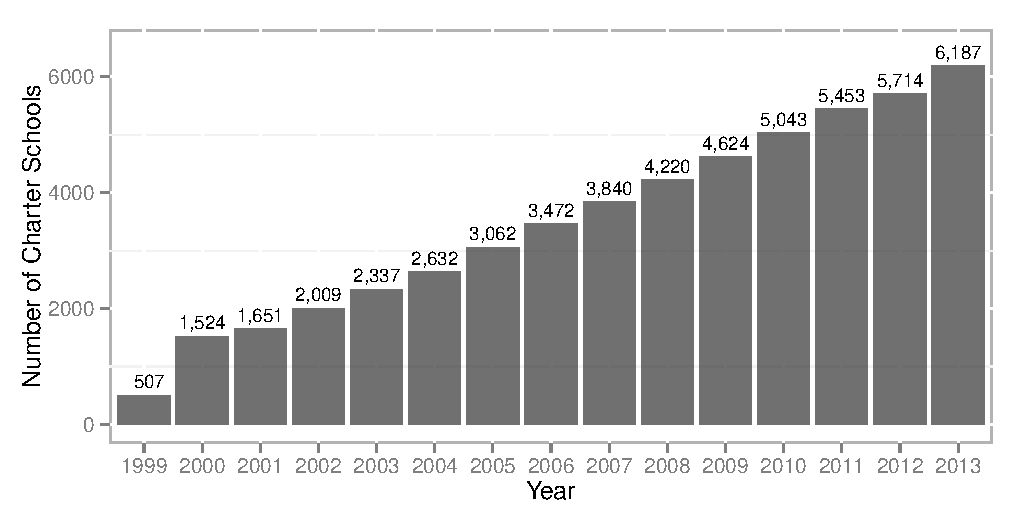
\includegraphics[width=\textwidth]{../Figures/CharterSchoolGrowth.pdf}
\caption{Charter school growth 1999-2013}
\label{fig:charterSchoolGrowth}
\end{figure}

%Clearly charter schools have become a popular vehicle for educational reform among parents as well. The \citeA{cersurvey} reports that 59\% of charter schools have waiting lists averaging 198 students. Charter schools provide an apparent choice to parents and are copacetic to the United State's individualistic culture \cite{hofstede2004,maccall1847,swart1962}. Moreover, like so many other fields, school reform has further emphasized marketization and privatization \cite{wells2002}. The influence of capitalism on education is not new. A major contributor to the expanded role of education during the industrial revolution is capitalism itself. That is, education expanded its initial purpose of providing a minimally informed electorate to providing an educated work force, not to mention keeping children off the streets as child labor laws came into existence. However, the shift of capitalistic principles from being the inspiration of educational reform to being the educational reform has profound implications.

%Proponents of charter schools argue that public schools have been bogged down by bureaucracy and union contracts. Freeing schools of these requirements then allows teachers and schools to innovate, which in theory leads to increased student performance. The principled argument is the ``market metaphor" \cite{wells2002}. That is, if schools were forced to compete for ``customers" (i.e. students), then the differentiating factor between schools would be their quality of education. 

%Opponents on the other hand have questioned the accountability, equity, effectiveness, and sustainability of charter schools. Several studies have shown that charter schools are not only failing to increase student performance, in many instances they are performing well under their traditional public school counterparts \cite<see e.g.,>{credo,BraunJenkinsGrigg2006,aft2004}. Still, others argue whether charter schools may be a solution in search of a problem. \citeA{carnoy2005} in summarizing the controversy that ensued after the \citeA{aft2004} study argue that:

%%
Charter schools have become a popular vehicle for educational reform among parents. The \citeA{cersurvey} reports that 59\% of charter schools have waiting lists averaging 198 students. Charter schools provide an apparent choice to parents and are copacetic to the United State's individualistic culture \cite{hofstede2004,maccall1847,swart1962}. 

Like so many other fields, school reform has further emphasized marketization and privatization \cite{wells2002}. The influence of capitalism on education is not new. A major contributor to the expanded role of education during the industrial revolution is capitalism itself. That is, education expanded its initial purpose of providing a minimally informed electorate to providing an educated work force, not to mention keeping children off the streets as child labor laws came into existence. However, the shift of capitalistic principles from being the inspiration of educational reform to being the educational reform has profound implications. Proponents of charter schools argue that public schools have been bogged down by bureaucracy and union contracts. Freeing schools of these requirements then allows teachers and schools to innovate which, in theory, leads to increased student performance. The principled argument is the ``market metaphor" \cite{wells2002}. That is, if schools were forced to compete for ``customers" (i.e. students), then the differentiating factor between schools would be their quality of education. 

Opponents, on the other hand, have questioned the accountability, equity, effectiveness, and sustainability of charter schools. Several studies have shown that charter schools are not only failing to increase student performance, but in many instances are performing well below their traditional public school counterparts \cite<see e.g.,>{credo,BraunJenkinsGrigg2006,aft2004}. 

Others argue that charter schools may be a solution in search of a problem. \citeA{carnoy2005}, in summarizing the controversy that ensued after the \citeA{aft2004} study argue that:

\begin{quote} \normalsize
If, however, charter schools are not improving the achievement of disadvantages children, it may be that the cause of low student performance is not bureaucratic rules but something else. When a treatment is based on a diagnosis, and the treatment doesn't work, it is prudent to examine not only whether the treatment should be improved, but also whether the diagnosis might be flawed. \cite{carnoy2005}
\end{quote}

% TODO: Please follow this quote with an explanation of the diagnosis you think is appropriate, if relevant to the topic of your study. Then write a transition to the discussion of the research. 


\subsection{Statement of the Problem}
The issues surrounding charter schools are large in scope. However, given the implications for the current and future generations of students, the question must be explored using the best data and methods available. As \citeA{BettsHill2006} point out, there are three major obstacles to addressing the question of ``whether students in charter schools are learning more or less than they would have learned in conventional schools" (p. 1), namely:

\begin{enumerate}
\item The issues of counterfactuals. That is, there are several barriers to determine the causal relationship between school choice and learning, most significantly the fact that students and families self-select to attend charter schools.
\item The variation in types of charter schools.
\item The nature of student achievement. Research has shown there are many other factors that contribute to student success including, but not limited to, socioeconomic status, parents education, student motivation, etc. The ability to decipher how school choice contributes to student learning in the context of all the other factors proves difficult.
\end{enumerate}

\noindent Though these issues are significant, they can be reasonably addressed. I will not claim to fully account for these issues, but I will attempt to address these issues using the best data and methods available while clearly stating the limitations.

Issue one will be dealt with in more detail in chapter three. However, in short, the propensity score analysis (PSA) used for this study is arguably, assuming proper implementation, the best approach to estimating causal inferences short of well designed randomized experiments. Of course in the context of an observational study the fundamental problem of causal inference remains \cite{Holland1986}, but limitations of this will be addressed.

The issue of charter school variation is often cited in critiques of national or large scale charter school studies. Given that the charter school debate is a national debate with implications at the Federal level as exemplified by the \textit{No Child Left Behind} legislation of the George W. Bush Administration and the \textit{Race to the Top} policy of the Barak Obama Adminsitration, large scales studies are not only necessary, they are critical. If charter schools are to be offered as an alternative to traditional public schools, then charter schools as a whole must be evaluated against public schools as a whole. More specifically, it is important not to evaluate whether a particular charter school, or type of charter school, is better, but whether the entire charter school concept is a better approach for educational reform.

Lastly, the environmental, social, community, and cultural factors that contribute to a student's academic achievement are often significantly underestimated. Often educational reform, as exemplified by the \textit{No Child Left Behind} Act and \textit{Race to the Top}, often places the responsibility solely on the school without consideration of the context in which the school operates. I am encouraged by President Obama's remarks to his first Joint Session of Congress \cite{Obama2009}:

\begin{quote} \normalsize
These education policies will open the doors of opportunity for our children. But it is up to us to ensure they walk through them. In the end, there is no program or policy that can substitute for a mother or father who will attend those parent/teacher conferences, or help with homework after dinner, or turn off the TV, put away the video games, and read to their child. I speak to you not just as a President, but as a father when I say that responsibility for our children's education must begin at home.
\end{quote}

\noindent Though I must be acutely aware and acknowledge the fact that schools are merely one factor of many that contribute to a students academic achievement, it does not preclude us from evaluating schools for their part. Similar to issue one, I argue that PSA provides an approach to best approximate the effects of school choice.

%\subsection{Guiding Research Questions}
%Given that charter schools are being offered as a solution for the needed educational reform nationally, it is imperative that they be evaluated from a national perspective. This study proposes to compare the academic performance in two domains of charter schools and public schools using the National Assessment of Educational Progress and propensity score analysis. More specifically, this study proposes to address the question: Are there differences between charter and public schools? And if so, what is the nature and extent of those differences?

%Moreover, this study proposes a new approach to propensity score analysis with multilevel data. Given that states have varying laws regarding how charter schools operate, data analysis should account for those potential systematic differences. The development of the \texttt{multilevelPSA} R package will provide methods to estimate and visualize the propensity score results both within states as well as provide an overall national estimate. Additionally, this study will introduce this new class of propensity score method within the context of two well established approaches, stratification and matching, where the former does not directly account for multilevel data and the latter makes indirect, partial, and implicit, adjustment for clustering. Lastly, I will emphasize and show the importance of visualizations to interpret all aspects of propensity score analysis.

\subsection{Purpose of the Study}
 
In order to explore the differences in performance between charter and traditional public schools, a secondary purpose of this study is the development of a new set of methods for propensity score analysis with multilevel, or clustered, data. One of these aims is to show how graphics can be used to address research questions in the context of multilevel propensity score analysis; another is to describe and illustrate the key features of a new package of R functions to facilitate multilevel propensity score analyses, vis-\`{a}-vis the \texttt{multilevelPSA} package in R. Moreover, these new multilevel methods for propensity score analysis will be presented within the context of more traditional methods for propensity score analysis, namely stratification and matching. Not only will this show how these new methods perform with regard to more established methods, they may show with the use of modern graphics, how clusters may vary. 

The newly developed \texttt{multilevelPSA} package will be shown to provide an effective means of estimating and visualizing propensity score results with clustered (multilevel) data (these procedures are discussed more fully in chapters three and four). Moreover, the use of pre-existing visualization procedures such as loess regression plots, density plots, as well as the PSA balance and assessment plots introduced by \citeA{HelmreichPruzek2009}, can provide critical insight into the analysis and eventual interpretation of results. More succinctly, the presentation of graphics in this study are not merely provided for diagnostic or descriptive purposes, but are a critical component of presenting, analyzing, and interpreting results. For instance, related to research questions two and three below, it is the graphics that will be most revealing in the differences, if any, and not the numerical analyses (though numerical analyses are provided).

With the proliferation of charter schools nationally and the differences in state laws regarding how charter schools are created and operate, the impact of state laws on school performance is an important issue to consider. The National Alliance for Public Charter Schools (NAPCS) publishes rankings of state charter school laws \cite{NAPCS2012} each year. Given that the methods developed here will allow for explicit adjustment, or clustering, for state, the relationship between charter school performance and state laws will be explored.

Given that charter schools are regularly being offered as solutions for needed educational reform nationally, it is imperative that they be evaluated from a national perspective. This study proposes to compare the academic performance in two domains of charter and traditional public schools using the National Assessment of Educational Progress (NAEP) using multiple propensity score methods. More specifically, this study proposes to address the questions:

\begin{enumerate} 
	\item Given appropriate adjustments based on available student data, is there a discernible difference between charter and traditional public schools with regard to math and reading scores evaluated at grades 4 and 8?
	\item If so, what is the nature and magnitude of this difference for the two outcomes, reading and mathematics?
	\item And finally, what is the impact, if any, of different charter school laws on charter school student performance?
\end{enumerate}



%==================== CHAPTER 2 ====================================================================
\cleardoublepage
\section{Chapter 2: Review of the Literature}

Though Professor Ray Budde is often credited with the current charter school movement \cite{Kolderie2005}, the term \textit{school choice} can be traced back to Adam Smith's \textit{Wealth of Nations}, Thomas Paine's \textit{Rights of Man}, and John Stuart Mill's \textit{On Liberty} \cite{herbst2006}. Prior to the Revolutionary War, given the religious diversity of colonial America, issues of education were left to local communities. However, after the war, Revolutionary leaders argued that local schools were no longer sufficient for educating students for the emerging state and federal governments. It was Thomas Jefferson who, in 1779, introduced the first bill in Virginia that would establish a public school system. It was Jefferson, along with numerous other American intellects during the 1780s and 1790s, that established public schools throughout the young nation, thereby relegating school choice to a choice between public schools and predominately religious private schools.

In the wake of the landmark report \textit{A Nation at Risk} \cite{nationatrisk}, \citeA{Budde1988} authored a pivotal document that started the charter school movement in the United States. In this document, Budde argues that system-wide changes to the way schools are structured are required, including: more rigorous curriculum and graduation standards; extended school days and year; more homework; teacher accountability for student results; termination of ``incompetent" teachers; and higher pay for teachers. To achieve these goals, he proposed a fundamental change to the ``internal organization of the school district... making substantial changes in the roles of teachers, principals, the superintedent, the school board, parents, and others in the community" (p. 16). More specifically, a framework for charter schools was proposed that includes five stages over a three year period (see Figure \ref{fig:timeline}). The five stages include: (1) generating ideas; (2) planning the charter; (3) preparing for teaching; (4) teaching under the educational charter; and (5) program monitoring and evaluation. For the first iteration of the cycle, stages one, two, and three occur prior to the opening of the school with stage one ideally beginning a full school year before. 

There are several features of this framework that deviate from traditional public school models, most notably the repetition of what may appear to be preparatory stages. That is, the charter school personnel must re-plan their school structure periodically (every three to five years according to Budde's framework) in a manner consistent with the initial charter school creation, thereby forcing a re-evaluation of the school bureaucracy.

\begin{figure}[tp]
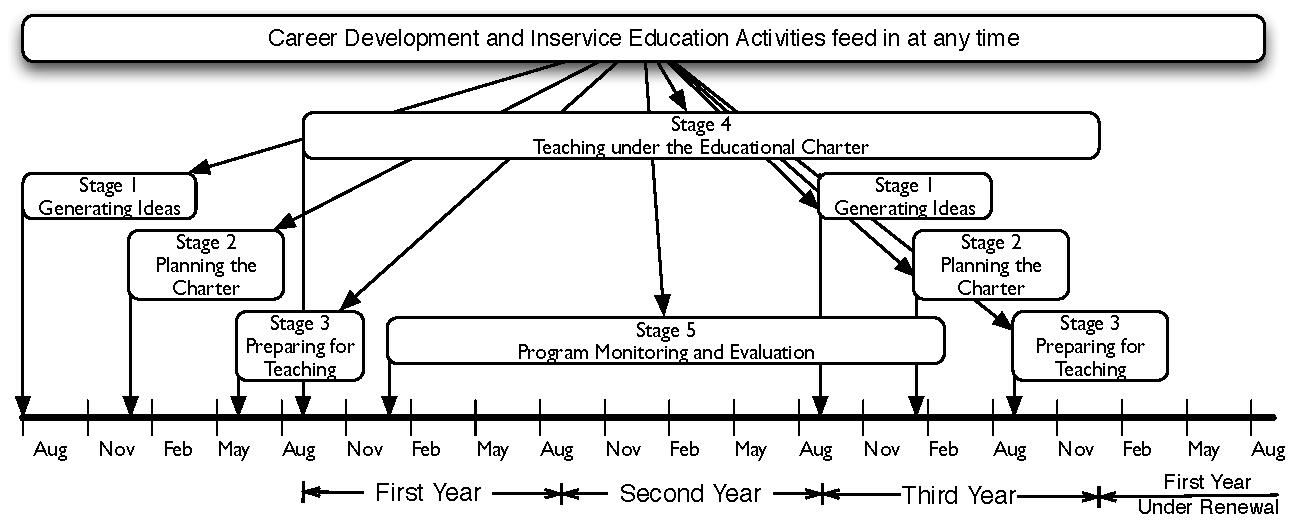
\includegraphics[width=\textwidth]{../Figures/Timeline.pdf}
\caption{Stages of a charter school life cycle (adapted from Budde, 1988)}
\label{fig:timeline}
\end{figure}

Following the suggestions of Budde, Minnesota passed the first charter school law in 1991 with California following in 1992. As of spring 2009, 40 states and the District of Columbia had charter school laws which comprise 1,407,421 students in 4,578 schools \cite{cernumbers}. 


\subsection{Empirical Evidence for Charter School Effectiveness}

According to \citeA{whatweknow}, there are currently over 200 studies that examine charter school achievement. The \citeA{whatweknow} provide a review of 140 studies selected on several criteria. Their review reveals significant gaps in the research with regard to states evaluated, research quality that addresses achievement, as well as timeliness of results. This is further exemplified by a meta-analysis conducted by \citeA{BettsTang2008} that includes just 13 studies that represent nine states. In this section I will provide an overview of the current literature available vis-\`{a}-vis the published meta-analysis and literature reviews. I then focus on two recent studies that together provide the context for the study proposed here: a hierarchical linear modeling analysis of the 2005 NAEP study \cite{BraunJenkinsGrigg2006} and a matching study comparing charter and public schools in 2009 in 16 states \cite{credo} and again in 2013 in 27 states \cite{credo2013}.


\subsubsection{Overview of Current Studies}

Research has shown that parents of students in charter schools are generally more satisfied with the charter school than the public school and will also tend to be more involved in their child's education \cite{TeskeSchneider2001,VanourekMannoFinnBierlein1998}. However, their satisfaction may simply be a rationalization \cite{HubbardKulkarni2009}. Moreover, Fuller et al. \cite<1996, as cited in>{HubbardKulkarni2009} suggest that parents that choose charter schools ``believe that the charter must therefore be superior to a conventional public school" (p. 177). This is reinforced by a study conducted by \citeA{CullenJacobLevitt2005} that examines school choice in Chicago Public Schools, where more than half of the students elect to attend a public school (e.g. career academy, high-achieving school) other than their locally assigned school. Though students who opt out of their local school are more likely to graduate, \citeA{CullenJacobLevitt2005} argue that ``those who opt out are superior along unobservable dimensions such as their motivation level and parental involvement" (p. 755). 

The \citeA{whatweknow} provides perhaps the most comprehensive review of available research on charter school performance. The current report, \textit{Charter School Achievement: What We Know} is now in its fifth edition, having been updated periodically to account for recent studies. In addition to covering published research reports, the review includes unpublished reports including conference presentations, dissertations, policy group and think tank reports, and state evaluations. Of the 210 studies identified in the fifth edition, 140 are included in their review. These 140 studies were determined to compare charter schools with traditional public schools, use ``serious research methods" (p. 2), and examine ``a significant segment of the charter sector" (p. X). The studies are then further classified into one of three categories: (1) panel studies that are longitudinal and examine student growth over time; (2) cohort change studies that are longitudinal but use some method other than tracking individual students; and (3) snapshot studies that examine school performance at a single point in time (also known as observational studies).

Table \ref{charterAchievement} summarizes the findings of the 140 studies included, first by breaking out the year(s) upon which the study's data is based, and second by the results reported. It should be noted that many of the pre-2001 studies were concentrated in a few states (Arizona, California, Florida, North Carolina, and Texas). This is expected, given that these states are among the earliest to adopt charter school laws (see Appendix A) as well as the substantial increase in the number of charter schools since 2000 (see Figure \ref{fig:charterSchoolGrowth}). The National Alliance of Public Charter Schools conclude that:

\begin{quote} \normalsize
[I]t becomes dramatically clear that studies examining public charter schools in more recent academic years show that charter schools produce more instances of larger achievement gains in both math and reading when compared to traditional public schools. (p. 3)
\end{quote}

\noindent However, this interpretation downplays the fact that approximately 30\% of charter schools performed worse than their traditional public school counterpart. These results are consistent with a recent study by the \citeA{credo} that reported that 37\% of charter schools performed worse than their public school counterpart in 2009 and 31\% in 2013.



\begin{table}
\caption{Summary of studies on charter school achievement}
\label{charterAchievement}
\begin{center}
\begin{tabular}{lrrrrrrrrrr}
\thickline
            & \multicolumn{4}{c}{Pre 2001} & & \multicolumn{4}{c}{Post 2001}\\
            \cline{2-5} \cline{7-10}
            & Larger   & Similar   & Mixed    & Smaller    & & Larger    & Similar   & Mixed    & Smaller\\
            & Gains    & Gains     & Gains    & Gains      & & Gains     & Gains     & Gains    & Gains\\
\hline
Math        & 4      & 4      & 4      & 20     & & 17     & 17     & 1      & 14\\
            & (13\%) & (13\%) & (13\%) & (63\%) & & (35\%) & (35\%) &  (2\%) & (29\%)\\
Reading     & 7      & 10     & 3      & 14     & & 18     & 12     & 1      & 14\\
            & (21\%) & (29\%) &  (9\%) & (41\%) & & (40\%) & (27\%) &  (2\%) & (31\%)\\
\thickline
\multicolumn{10}{l}{Source: National Alliance of Public Charter Schools, 2009}\\
\end{tabular}
\end{center}
\end{table}

\citeA{BettsTang2008} employ more stringent selection criteria for including studies in their meta-analysis. Only studies that used experimental, student-level, growth-based methods were included, resulting in a total of 14 studies published between 2001 and 2007 utilizing data ranging from 1998 through 2005. Similar to the review produced by the \citeA{whatweknow}, the studies were done in a limited number of locations, including Arizona, California (three from San Diego), Chicago, Delaware, Florida, Idaho, North Carolina, and Texas, with one anonymous location. Overall, the analysis of the available studies provide very mixed results. However, some patterns emerge, specifically that charter schools generally outperform traditional public schools in elementary school reading and middle school math, although effect sizes for the latter are small. Charter schools are generally underperforming traditional public schools in high school reading and math, but it should be noted that studies examining these grade levels are relatively small \cite<see also,>{whatweknow}.

% TODO: Brief summary paragraph, e.g., I hate to admit it but, in general, large-scale studies and reviews show that charter schools aren't all bad afterall… or something like that, followed by, however, many of the studies are limited by inappropriate statistical analyses [this latter part is important, as it begins to set up the need for your study, which is the main purpose of a lit review].

\subsubsection{Two NAEP Studies Using HLM}

In the context of the charter school question, comparing students in charter schools to public school counterparts with, for example, ordinary least squares or ANOVA, is inappropriate since these statistical models do not account for the school effects. HLM provides a model with which school effects can be partitioned from student effects, thereby providing adjustments for the lack of independence of observations \cite<see e.g.,>{BrykRaudenbush1992,GelmanHill2006}.

Braun, Jenkins, and Grigg have published two research reports utilizing NAEP data and HLM analyses that look at how public school students' test scores compare to those of private school students \citeyear{BraunJenkinsGrigg2006private} and charter schools students \citeyear{BraunJenkinsGrigg2006}. The former study used the 2005 administration of the NAEP, whereas the latter used the 2003 administration. A key advantage of using NAEP is that many student and school level variables are available (see Appendix C). Moreover, as of 2003 charter schools have been oversampled to ensure sufficient sample sizes for appropriate comparisons. 

\paragraph{Comparing private and public school students' NAEP scores} For the private school study \cite{BraunJenkinsGrigg2006private}, results suggest that students in private schools scored significantly higher than public school students in both mathematics and reading at grades 4 and 8. Differences ranged from 8 points for grade 4 mathematics to 18 points for grade 8 reading. Adjusting for student characteristics such as gender, ethnicity, and proxies for social economic status with HLM resulted in reductions in all four comparisons of approximately 11 to 14 points. After adjustment, private school students still scored significantly higher than public school students in grade 8 reading, but public schools scored significantly better in grade 4 mathematics. There was no significant difference for grade 4 reading and grade 8 mathematics.

\paragraph{Comparing charter and public school students' NAEP scores}
For the charter school study \cite{BraunJenkinsGrigg2006}, the analysis was conducted in three phases for both reading and mathematics. In phase one, all sampled charter schools were compared to all sampled public schools. Results suggest that, when student characteristics were adjusted for, charter schools performed, on average, 4.2 points lower than publics schools in reading (effect size is 0.11 standard deviations) and 4.7 points lower in mathematics (effect size is 0.17 standard deviations). 

Phase two separated charter schools into two groups: charter schools that are associated with a public school district (PSD) and those that were not. For reading, there was no significant difference between charter schools affiliated with a PSD and public schools. However, for schools not affiliated with a PSD, charter school students scored significantly lower than public school students, with an adjusted difference of 0.17 standard deviations. For mathematics, there was no difference between charter schools affiliated with a PSD and public schools, but charter schools not affiliated with PSD scored significantly lower, with an adjusted difference of 0.23 standard deviations.

Phase three compared only charter and publics schools located in a central city and serving a high-minority population. For reading, there was no significant difference between charter and public schools for any model. For mathematics, however, charter schools not affiliated with a PSD scored significantly lower than public school students with an adjusted difference of 0.17 standard deviations. There was no difference for schools affiliated with a PSD. 

\cite{BraunJenkinsGrigg2006} concluded that, after adjusting for student characteristics, that charter school mean scores were lower than traditional public school with the larger differences being in reading. Moreover, some of the variation in mean school performance could be attributed to other characteristics such as policies from which the school had waivers or exemptions, student population served, and program content.

%\clearpage

\subsubsection{The CREDO Study}

The \citeA{credo,credo2013} conducted a study of more than 1.7 million records from 2400 charter schools within 16 and 27 states in 2009 and 2013, respectively. The methodology involves creating a Virtual Control Record (VCR) for each charter school student \cite<see also,>{AbadieDiamondHainueller2007,nea} which is used to find matching students from an eligible traditional public school. Students within a traditional public school become available in a pool of potential matches when at least one student is identified as transferring to a charter school. Once the ``feeder schools" are identified, all students from feeder schools are pooled and serve as the source to select matches to the charter school students. Students are then matched on the following factors: grade-level, gender\footnote{Gender was not available in Florida}, race/ethnicity, free or reduced price lunch status, English language learner status, special education status, and prior test score on state achievement tests. This procedure, which is similar to propensity matching, resulted in 83.7\% and 84.4\% of charter school students being matched to a public school student for reading and math, respectively.

Once matches were determined, ordinary least squares regression was utilized to analyze both math and reading scores of the charter school students and matched public school students separately. Moreover, controls for student characteristics, excluding gender, along with state indicators and scores affected by Hurricane Katrina, were added to the basic model. Overall results showed that charter school students performed, on average, 0.01 and 0.03 standard deviations below public school students for reading and math, respectively. Both results are significant at \textit{p} $\leq$ 0.01.

Further analysis by \citeA{credo} revealed that the effectiveness of charter schools varied considerably by state. Five states (Arkansas, Colorado, Illinois, Louisiana, and Missouri) were found to have higher learning gains for charter schools. Six states (Arizona, Florida, Minnesota, New Mexico, Ohio, and Texas) were found to have lower learning gains for charter schools. The remaining four states (California, District of Columbia, Georgia, and North Carolina) had either mixed results or no difference in academic gains. The new methods developed for this study will also explicitly account for the variation between states to provide insight into implications of the varied policy environments charter schools operate in.

The \citeA{credo} also found variation in charter school effectiveness across school characteristics. That is, schools that focused on elementary or middle grades separately tended to perform as well or better than their public school counterparts. However, for charter schools that focused on high grades or multi-level grades performed anywhere from .02 to .08 standard deviations below public schools. Moreover, school level comparisons find that only 17\% of charter schools performed better than public schools while 46\% perform no differently and 37\% perform significantly worse.

The results from the 2013 study \cite{credo2013} showed a small increase in the differences between charter and traditional public school students. The Center for Research on Education Outcomes prefers to present their results in a metric of days. In 2009, charter school students had a loss of 7 school days which increased to a gain of 8 school days in 2013. For math, charter school students has a loss of 22 days in 2009 and are on par with traditional public school students in 2013.  Reporting in terms of days is problematic since it is difficult to compare to other studies. However, these differences reported as effect sizes are approximately between 0.01 and 0.03 \cite{Loveless2013}. These results, as will be shown in chapter four, are consistent with the results of this study. Moreover, this also demonstrates an issue with null hypothesis testing and p-values, especially with large a \textit{n}. 

% Possible TODO: add footnote on how to convert between effect size and days

\subsection{Propensity Score Analysis}

Randomized experiments are the \textit{gold standard} for estimating causal effects of a treatment. However, as is frequently the case in educational contexts, randomization for the current project is neither ethical nor feasible. Therefore, propensity score methods \cite{RosenbaumRubin1983} using matching \cite{StuartRubin2008,Stuart2010} and stratification methods \cite{RaudenbushHongRowan2003} will be used to make quasi-experimental estimates of causal effects \cite<see also>{SchneiderEtAl2007,StuartRubin2008}. Recent research comparing the use of propensity score methods with randomized experiments have shown that causal estimates from observational studies using propensity score methods are generally consistent with those from randomized experiments \cite{CookShadishWong2008,ShadishClarkSteiner2008}. The use of propensity score methods in published research in psychology and education has been growing over the last decade \cite{ThoemmesKim2011}.

The selection of covariates is particularly challenging in propensity score analysis. As such, multiple methods for the estimation of propensity scores will be used \cite{Rosenbaum2012}. The goal in the estimation of propensity scores is to reduce selection bias, therefore simple significance testing is not appropriate \cite{Rosenbaum2002} since potentially non-significant covariates may be proxies for important non-observed covariates. Although this study has been designed to measure the same covariates as would be used in a randomized block design, multiple methods utilizing varying number of covariates will be used. Moreover, we wish to provide overall effect sizes but also measure the effects of clustering by state. 

Although propensity score analysis has been shown to provide estimates consistent with randomized experiments \cite{ShadishClarkSteiner2008,DehejiaWahba1999,HeckmanEtAl1997}, its use has not been immune to criticism \cite<c.f.>{Shadish2013}. \citeA{Pearl2009} has raised concerns about a potential increase in bias due to the inclusion of certain covariates in the estimation of propensity scores in response to \citeauthor{Rosenbaum2002}'s \citeyear{Rosenbaum2002} suggestion that, in general, the inclusion of all observable covariates is preferable to excluding them. However, Pearl's concerns can be mitigated in at least three ways. First, careful checking of balance across all observable covariates is done even if the covariate is not used in the modeling of the propensity scores. Second, sensitivity analysis \cite{Rosenbaum2002} can be conducted after matching to consider the question of whether the estimate would differ in the presence of additional unobserved covariates. That is, sensitivity analysis tests the robustness of the propensity score estimation for hidden bias. However, sensitivity analysis is only well defined for one-to-one matching and therefore is not used in this study. Third, multiple methods can be utilized for estimating propensity scores \cite{Rosenbaum2012}. Specifically, in addition to matching based upon propensity scores estimated from logistic regression, stratification methods using both quintiles on the logistic regression estimated propensity scores and classification trees provide parametric and non-parametric estimates, respectively. 

The use of propensity score methods is still preferable over traditional regression models in spite of \citeauthor{Pearl2009}'s \citeyear{Pearl2009}  criticisms. Propensity score analysis separates the covariates related to selection bias and the comparison of the outcome of interest. This clean separation of the research design also provides a clear interpretation of results similar to randomized experiments. As will be discussed more fully in chapter three, special emphasis must be placed on achieving balance. In the context of propensity score analysis, balance refers to reducing bias or differences between observed covariates for the units that will be compared. For example, if after matching you find that each matched pair has the same ethnicity, you would conclude that perfect balance has been achieved for that covariate. In chapter three I will outline a number of approaches for checking balance for both matching and stratification methods. Although there is the possibility of a lack of balance in an unobserved covariate (i.e. ``hidden bias"), this would similarly affect regression methods and is admittedly an important limitation of any non-randomized method for estimating causal effects. However, NAEP is designed to include most, if not all, the important covariates one would expect to be related to charter school attendance (see Appendix B for descriptive statistics for all the covariates used in this study).

\subsection{Research Questions}

Clearly charter schools have become a significant part of education in the United States. Given their position as an alternative to traditional public schools, it is important to have good research about their effectiveness. Given that randomized trials are not possible, propensity score methods provide the best alternative to providing causal estimates of the differences between students who attend charter schools and their traditional public school counterpart. Moreover, the new methods developed for this study will provide further insight into the extent of the variation among charter schools as well as the variation between states. As such, this study will address the following research questions:

\begin{enumerate}
\item Given appropriate adjustments based on available student data, is there a discernible difference between charter and traditional public schools with regard to math and reading scores on the NAEP evaluated at grades 4 and 8?  
\item If so, what is the nature and magnitude of this difference for the two outcomes, reading and mathematics?  
\item What is the impact, if any, of different charter school laws on charter school student performance?  
\end{enumerate}

%==================== CHAPTER 3 ====================================================================
\cleardoublepage
\section{Chapter 3: Method}

This chapter will outline the methods that will be utilized to describe and analyze the data in order to address the research questions central to this study. Given the strong political interests in the question of charter school effectiveness and the implications for educational policy both at the state and national level, obtaining good empirical evidence, preferably with strong causal inferences, is most desirable. The \textit{gold standard} of inferential research is the randomized experiment. A research design that addresses the charter school question proposed here would require that students be randomly assigned, possibly with blocking on key covariates, to either a charter or public school. The theoretical justification for such a scheme is that any systematic differences between the two groups would be balanced through the randomization processes. However, in practice, especially in education, such randomization is neither feasible nor ethical. The result of the lack of randomization is a phenomenon called selection bias. That is, any comparisons of the two groups will be biased given the fact that the units of study, in this case students, self-selected to be in their respective group. Propensity score analysis \cite{RosenbaumRubin1983} is a statistical approach whereby the observed differences between the two groups are balanced by the careful analysis of covariate information. This procedure lends itself well to secondary analysis of observational data.

I have written and published two R packages primarily for conducting the analysis in this dissertation. The \texttt{naep} package provides functions to read and work with the National Assessment of Educational Progress (NAEP) data sets. Secondly, the \texttt{multilevelPSA} package provides functions to conduct multilevel propensity score analysis as described below. Both of these packages are available from the Comprehensive R Archive Network (CRAN). 

\textit{Formatting note}. Since the development of the R packages are in and of themselves a major component of this dissertation, I will make reference to some of the functions available. By convention, all references to R packages and functions will appear in a \texttt{fixed width font}.

\subsection{Overview of NAEP}

The source of the data that will be utilized in this study is the National Center for Educational Statistics (NCES), which is within the U.S. Department of Education's Institute of Education Sciences (IES). The National Assessment of Educational Progress (NAEP) was started in 1971 and has provided national measures of student achievement in many subjects including mathematics, reading, science, writing, history, civics, and the arts. In 2003 NAEP began assessing charter schools as well as private and public schools. This study will utilize the 2007 administeration of the NAEP assessments in mathematics and reading in grades four and eight. The 2007 assessment included over 6,000 public schools and over 200 charter schools comprising over 145,000 and 3,000 students, respectively. Given this large, nationally representative sample, analysis of NAEP assessments utilizing propensity score analysis may provide valuable insights into the academic differences between charter and public schools, should they exist.

Another key advantage of NAEP is the fact that it is not designed to assess individual students or schools, but rather to inform subject-matter achievement, instructional experiences, and school environments \cite{BraunJenkinsGrigg2006}. To achieve this goal, NAEP utilizes a complex item-sampling design such that individual students are presented a subset of the total items, thereby reducing the burden on participants. Though not appropriate for assessing individual student achievement, in aggregate, the NAEP measures provide a robust and accurate estimate of student achievement.

In addition to subject area measures, NAEP includes student, teacher, and school questionnaires that provide contextual information about the learning environment. Given that PSA relies on adjusting for selection bias by adjusting for known covariates, it is the answers to these questionnaires that will serve as the basis for determining a student's propensity score, or likelihood of being in the treatment (charter school in the context of this study). In addition to typical demographic items such as gender and race, students are asked about computers, books, magazines, and encyclopedias in the home; parents' education level; and the level of interaction with academics within the home (see appendix C for complete list of items).

The responsibility for developing the assessment objectives and test specifications lies with the National Assessment Governing Board, which was created by Congress in 1988. The 26-member board is made up of governors, state legislators, local and state school officials, educators and researchers, business representatives, and members of the general public. Given the varied standards across states, it is this governing board that is to determine nationally what are appropriate achievement goals for each age and grade. The following two sections will provide the framework for mathematics and reading assessments.

\subsubsection{Mathematics}

Since 1990, the Council of Chief State School Officers (CCSSO) has been contracted to design a framework for the mathematics assessment \cite{naepmath}. The framework was most recently updated in 2000 to take into account state standards, the National Council of Teachers of Mathematics (NCTM) standards, the Trends in International Mathematics and Science Study (TIMSS), the Achieve Project, and a 2001 report issued by the National Research Council of the National Academy of Sciences. The result of their work was six recommendations for the mathematics assessment regarding content areas, mathematical complexity of items, distribution of items, item formats, manipulatives, and calculators. For the purposes of this study, a composite score will be utilized that is comprised of five content areas, number properties and operations; measurement; geometry; data analysis and probability; and algebra. Table \ref{naepMathContent} provides details regarding the distribution of items comprising the composite score for the grade four and eight assessments.

\begin{table}
\caption{Distribution of Math Items by Grade and Content Area}
\label{naepMathContent}
\begin{center}
\begin{tabular}{lrr}
\thickline
Content Area                     & Grade 4 & Grade 8\\ \hline
Number Properties and Operations & 40\%    & 20\% \\
Measurement                      & 20\%    & 15\% \\
Geometry                         & 15\%    & 20\% \\
Data Analysis and Probability    & 10\%    & 15\% \\
Algebra                          & 15\%    & 30\% \\
\thickline
\end{tabular}
\end{center}
\end{table}


\subsubsection{Reading}

The NAEP reading assessment \cite{naepreading} is designed to account for three reading contexts: reading for literacy experience, reading for information, and reading to perform a task. Within these contexts, four aspects of reading are considered: forming a general understanding, developing interpretation, making reader/text connections, and examining content and structure. The reading assessment is administered by supplying students with booklets that contain reading materials and comprehension questions. The questions consist of both multiple-choice and constructed-response question formats with at least half of the questions being of the constructed-response type. 

The \citeauthor{naepreading} NAEP Reading Framework (2006) provides guidelines and a theoretical basis for reading assessment. This framework is designed with the input of individuals and organizations involved in reading education including researchers, policymakers, teachers, and business representatives. However, a particular emphasis is placed on the work of the National Institute for Child Health and Human Development (NICHID). According to the NICHID  the cognitive research suggests that ``reading is purposeful and active. According to this view, a reader reads a text to understand what is read, to construct memory representations of what is understood, and to put this understanding to use" \cite<p. 4, NICHD, 2000, as cited in>{naepreading}. Moreover, reading is considered to be a complex process rather than a simple set of skills. As such, the NAEP reading assessment is designed such that comprehension is defined as: ``[I]ntentional thinking during which meaning is constructed through interactions between text and reader" (Harris \& Hodges, 1995). Thus, readers derive meaning from text when they engage in intentional, problem solving thinking processes" \cite<p. 14, NICHD, 2000, as cited in>{naepreading}. Given this framework, NAEP provides an excellent tool for evaluating overall reading achievement but not to diagnose specific individuals.

%\subsection{Sample}

%%TODO:

\subsection{Data Preparation}

The propensity score methods use the available covariates to adjust for selection bias. However, the geographic distribution of charter schools is not equal. That is, charter schools are more prevalent in certain geographic regions of the country, often within urban areas. Since there are several orders of magnitude difference in the number of charter school to traditional public school students, selecting a subset of all the traditional public school students available in NAEP is necessary. By selecting traditional public school students who live in close proximity to a charter school, the likelihood of the former actually choosing a charter school increases. According to the National Household Travel Study, students travel an average of five miles to school. The Common Core of Data \cite{ccd} provides the location of every public school in the United States. For each traditional public school, the distance to the closest charter school was calculated using line-of-sight distance. Within states that have charter schools, approximately 20\% of traditional public schools were more than five miles from a charter school. Those schools, and subsequently students attending those schools in any of the NAEP datasets, were eliminated from the study. Table \ref{dependentDescriptivesAllAndClose} provides descriptive statistics for charter school students, all public school students, and public school students within five miles on each of the outcome measures. It shows that there is not a substantial difference in the mean scores for traditional public school students and in fact, reduces the unadjusted differences between charter and traditional public school students.

% latex table generated in R 3.0.2 by xtable 1.7-1 package
% Wed Feb 19 10:32:31 2014
\begin{table}
\centering
\caption{Descriptive statistics of dependent variables (unadjusted) for all and close (within 5 miles) traditional public schools} 
\label{dependentDescriptivesAllAndClose}
\begin{tabular}{lr@{\extracolsep{.2cm}}rrr@{\extracolsep{.2cm}}rrr}
  \hline
   & \multicolumn{1}{c}{Charter} & \multicolumn{3}{c}{All Public Schools} & \multicolumn{3}{c}{Close Public Schools} \\ \cline{2-2} \cline{3-5} \cline{6-8}  Subject & Mean & Mean & n & Diff &  Mean & n & Diff \\  \hline
Grade 4 Math & 231.2 & 238.3 & 159338 & -6.9 & 237.3 & 85272 & -6.0 \\ 
  Grade 4 Reading & 212.9 & 218.8 & 168597 & -6.0 & 217.1 & 92756 & -4.2 \\ 
  Grade 8 Math & 272.8 & 280.7 & 152048 & -8.6 & 279.4 & 71528 & -7.5 \\ 
  Grade 8 Reading & 256.2 & 261.7 & 151304 & -5.5 & 259.8 & 73810 & -3.6 \\ 
   \hline
\end{tabular}
\end{table}


Appendix B provides descriptive statistics for all the covariates for the four datasets. Additionally, unadjusted differences in NAEP scores for each state containing a charter school are provided. Table \ref{dependentDescriptives} below provides the overall, unadjusted, differences in NAEP scorers for the four datasets.

% latex table generated in R 3.0.1 by xtable 1.7-1 package
% Tue Jun 11 07:43:51 2013
\begin{table}[ht]
\centering
\caption{Descriptive Statistics of Dependent Variables (Unadjusted)} 
\label{dependentDescriptives}
\begin{tabular}{lrr@{\extracolsep{.2cm}}rrrrr}
  \hline
   & \multicolumn{2}{c}{Charter} & \multicolumn{2}{c}{Public} & Mean & \multicolumn{2}{c}{Confidence} \\ \cline{2-3} \cline{4-5}  Subject & Mean & SD & Mean & SD & Difference & \multicolumn{2}{c}{Interval} \\  \hline
Grade 4 Math & 231.2 & 28.3 & 237.3 & 28.5 & -6.0 & -7.0 & -5.0 \\ 
  Grade 4 Reading & 212.9 & 33.0 & 217.1 & 34.5 & -4.2 & -5.3 & -3.1 \\ 
  Grade 8 Math & 271.8 & 35.5 & 279.4 & 35.8 & -7.5 & -8.7 & -6.4 \\ 
  Grade 8 Reading & 256.2 & 32.9 & 259.8 & 32.6 & -3.6 & -4.7 & -2.6 \\ 
   \hline
\end{tabular}
\end{table}


\subsection{Missing Data Imputation}

Logistic regression, which is one of the two ways propensity scores will be estimated, require a complete dataset for estimation. Appendix D provides figures created using the \texttt{missing.plot} function in the \texttt{multilevelPSA} package representing the extent of missingness for each covariate within each state. The first thing these figures reveal is that there is complete missingness in the majority of covariates for Alaska in grade four. As a result, Alaska was removed from all datasets and was not included in the study. 

Secondly, the figures show that there are fewer than 5\% of values missing for the vast majority of covariates. In grade four math and reading, the three exceptions are newspapers in home, magazines in home, and encyclopedia in home. Grade eight math and reading also show a higher rate of missingness in these three covariates, but also in parents' education level. To examine whether data is missing at random, a logistic regression model was estimated predicting treatment from a shadow matrix (i.e. a matrix with the same dimension of the original dataset with 0s and 1s where 1s indicate the value is missing). 

The results of these models indicate that there is no relationship between charter school attendance and whether a student completed items regarding newspapers, magazines, and encyclopedias in the home. However, for grade eight math and reading, missingness of mother's and father's education level were statistically significant (\textit{p} \textless .05) predictors of treatment. Charter school students' mother's education level was less likely to be missing whereas father's education level was less likely to be missing for traditional public schools. Although these two covariates are often important for understanding students' educational achievement, the figures in Appendix I depicting the relative importance of each covariate for predicting charter school attendance using conditional inference trees, which are estimated with missingness included, suggest that these covariates have relatively low, or no, predictive value for charter school attendance. Therefore, missing values for these covariates will be imputed and used to estimate propensity scores for the logistic regression and matching methods. It should also be noted that this variable was not collected from fourth grade students.

Multiple imputation \cite{rubin1987,Rubin1996mi} has become a popular approach for imputing missing values in datasets. For this study, missing data was imputed using multivariate imputation by chained equations vis-à-vis the MICE package \cite{mice,vanbuuren} in R. This package implements the fully conditional specification (FCS) method of imputation whereby separate multivariate imputation models are estimated for each variable containing missing values so that each model has its own set of conditional densities. Since the algorithm iterates through the data in small steps, providing the imputed values as it proceeds, the result is a robust estimate of imputed values. This study used both the original incomplete data for estimating propensity scores with classification trees and the complete imputed data for estimation propensity scores using logistic regression.


\subsection{Analysis}

This study utilizes propensity score analysis for estimating causal effects of students attending charter schools. The propensity score is ``the conditional probability of assignment to a particular treatment given a vector of observed covariates" \cite{RosenbaumRubin1983}. The probability of being in the treatment is defined as:

This study utilizes propensity score analysis for estimating causal effects of students attending charter schools. The propensity score is ``the conditional probability of assignment to a particular treatment given a vector of observed covariates" \cite{RosenbaumRubin1983}. The probability of being in the treatment is defined as:

$$\pi ({ X }_{ i }) \; \equiv \; Pr({ T }_{ i } = 1 | { X }_{ i })$$

\noindent Where $X$ is a matrix of observed covariates. The balancing property under exogeneity states that,

$${ T }_{ i } \; \upModels { X }_{ i } \;| \; \pi ({ X }_{ i })$$

\noindent In the case of randomized experiments, the strong ignobility assumption states,

$$({ Y }_{ i }(1),{ Y }_{ i }(0)) \; \upModels \; { T }_{ i }|{ X }_{ i }$$

\noindent for all ${X}_{i}$. That is, treatment is independent of all covariates, observed or otherwise. However, we can restate the strong ignobility assumption with the propensity score as,

$$({ Y }_{ i }(1),{ Y }_{ i }(0)) \; \upModels \; { T }_{ i } \; | \; \pi({ X }_{ i })$$

\noindent so that treatment placement is ignorable given the propensity score presuming sufficient balance\footnote{Balance in the context of PSA refers to differences in observed covariates between treatment and control units is minimized.} is achieved.

The average treatment effect (ATE) is defined as $E(r_1) - E(r_0)$ where $E(.)$ is the expected value in the population. Given a set of covariates, $X$, and outcomes $Y$, where 0 denotes traditional public school student and 1 denotes charter school student, ATE is defined as:

$$ATE=E(Y_{1}-Y_{0}|X)=E(Y_{1}|X)-E(Y_{0}|X)$$
 
\noindent Or the difference between charter and traditional public school given the set observed covariates.

\citeA{Rosenbaum2012} suggests that hypotheses should be tested more than once in observational study. This study will estimate treatment effects using nine separate propensity score models within three larger classes. The first two classes of PSA, stratification and matching, are well established in the PSA literature. The third class of PSA, multilevel PSA, and as implemented in the \texttt{multilevelPSA} R package, was developed for this dissertation. With these three classes of PSA, results will reflect: one, no adjustment for state (stratification), two, implicit adjustment for state (matching), and three, explicit adjustment for state (multilevel PSA). For each of the four subject and grade combinations, the following methods will be used, resulting in a total of 36 propensity score analyses being conducted.

\begin{enumerate}
\item Propensity score analysis using stratification. This method ignores state assignment as a clustering variable. Under this broader method three statistical methods for stratification will be used:
	\begin{enumerate}
	\item Full logistic regression. This method will estimate propensity scores using logistic regression with all available covariates, but will exclude interaction or product terms.
	\item Logistic regression with step AIC. The step AIC in the MASS package \cite{mass} will select the best logistic model based upon the Akaike Information Criterion \cite{Akaike1974}. In this case the ``best" first order interaction terms will be added to the main effect terms in (a).
	\item Conditional inference trees, based on all covariates; missing data will also be accommodated with the tree-based methods.
	\end{enumerate}
\item Propensity score matching. This method implicitly accounts for clustering. That is, the method used will find matches between charter and traditional school students that first match exactly on state, ethnicity, and gender, then finds a best match based upon the propensity scores estimated using logistic regression. As suggested by \citeA{Stuart2010}, multiple matched sets will be formed using:
	\begin{enumerate}
	\item One-to-one (i.e. one charter school student is matched to no more than one traditional public school student).
	\item One-to-five (i.e. one charter school student is matched to as many as five traditional public school students).
	\item One-to-ten (i.e. one charter school student is matched to as many as ten traditional public school students).
	\end{enumerate}
	A dependent sample analysis will be performed on the resulting matched pairs \citeA{Austin2011}.
\item Multilevel propensity score analysis \cite<see e.g.>{multilevelPSA}. This method will utilize the same stratification methods as described in method one above, namely:
	\begin{enumerate}
	\item Full logistic regression.
	\item Logistic regression with step AIC.
	\item Conditional inference trees.
	\end{enumerate}
\end{enumerate}


\subsubsection{Graphical Representation}

Given the large amount of data to be summarized, the use of graphics will be an integral component of representing the results. The \texttt{multilevelPSA}\footnote{The \texttt{multilevelPSA} package was written by the author and is available from \url{http://github.com/jbryer/multilevelPSA}.} package provides a number of graphing functions that extend the framework introduced by \citeA{HelmreichPruzek2009} for multilevel PSA. Figure \ref{fig:g8math:circ} represents a multilevel PSA assessment plot with annotations. This graphic represents the results of comparing private and public schools in North America using the Programme of International Student Assessment \cite<PISA;>{pisa}. The PISA data to create this graphic is included in the \texttt{multilevelPSA} package and a more detailed description of how to create this graphic are discussed at the end of this chapter. Additionally, the use of PISA will make more visible certain features of the graphics used. As will be discussed in chapters four and five, the differences between charter and traditional public schools is minimal and therefore some features of the figures will be less apparent. The following section will focus on the features of this graphic.

\begin{figure}[t]
\begin{center}
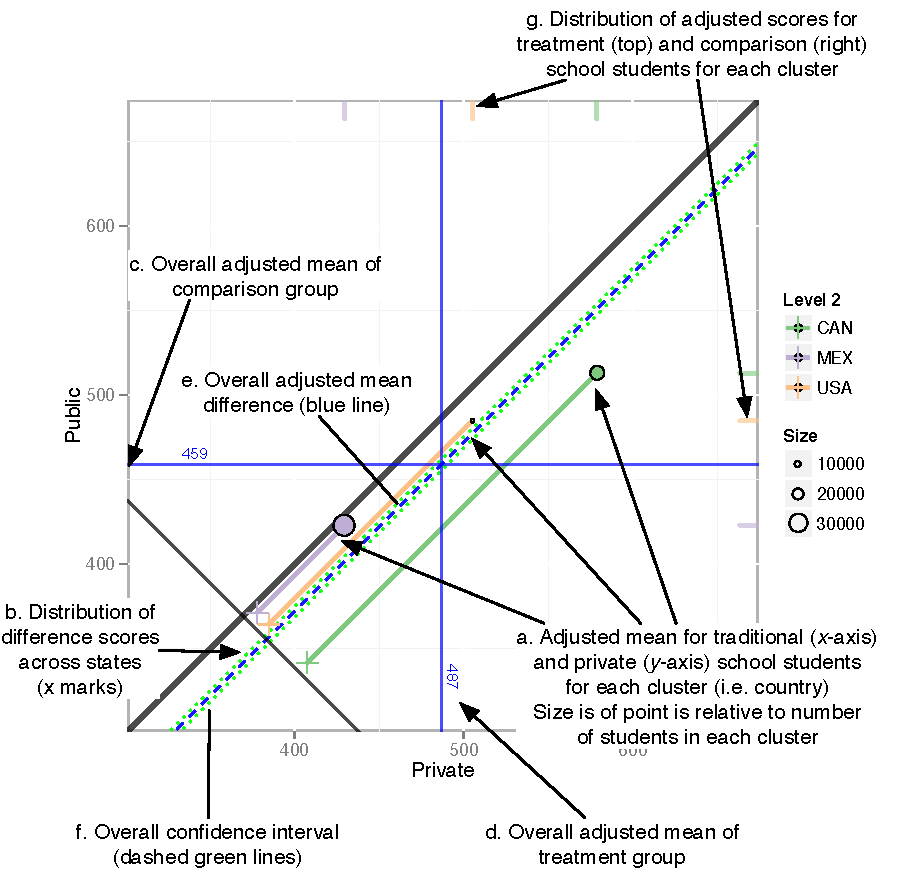
\includegraphics[width=.9\textwidth]{../Figures/AnnotatedCircPlot.pdf}
\caption{Annotated multilevel PSA assessment plot}
\label{fig:g8math:circ}
\end{center}
\end{figure}


In Figure \ref{fig:g8math:circ}, the x-axis corresponds to math scores for private schools and the y-axis corresponds to public school maths cores. Each colored circle (a) is a country with its size corresponding to the number of students sampled within each country. Each country is projected to the lower left, parallel to the unit line, such that a tick mark is placed on the line with slope -1 (b). These tick marks represent the distribution of differences between private and public schools across countries. Differences are aggregated (and weighted by size) across states. For math, the overall adjusted mean for private schools is 487, and the overall adjusted mean for public schools is 459 and represented by the horizontal (c) and vertical (d) blue lines, respectively. The dashed blue line parallel to the unit line (e) corresponds to the overall adjusted mean difference and likewise, the dashed green lines (f) correspond to the confidence interval. Lastly, rug plots along the right and top edges of the graphic (g) correspond to the distribution of each country's overall mean private and public school math scores, respectively.

Figure \ref{fig:g8math:circ} represents a large amount of data and provides insight into the data and results. The figure provides overall results that would be present in a traditional table, for instance the fact that the green dashed lines do not span the unit line (i.e. y = x) indicates that there is a statistically significant difference between the two groups. However additional information is difficult to convey in tabular format. For example, the rug plots indicate that the spread in the performance of both private and public schools across countries is large. We can also observe that Canada, which has the largest PISA scores for both groups, also has the largest difference (in favor of private schools) as represented by the larger distance from the unit line.


\subsection{The \texttt{multilevelPSA} R Package}


All of the analysis for this study were conducted using R \cite{rdevelopment}. The use of R provides a number of important advantages. First, all of the analyses are reproducible. That is, researchers can download all the R scripts\footnote{Available on Github at \url{https://github.com/jbryer/Dissertation}.} and those with access to the restricted NAEP data\footnote{Typically data is included for the analysis to be fully reproducible. However, given the sensitive nature of the data the National Center for Education Statistics (NCES) requires a restricted license for access to the data.} can run all the analyses. However, since NAEP is not readily available to anyone, PISA data will be used to demonstrate the features of the \texttt{multilevelPSA} package. Another important advantage of using R is that it is an extensible vis-\`{a}-vis R packages. Packages are collections of functions, data, and documentation designed for a specific purpose. Since the multilevel PSA methods described in this dissertation have never been conducted or implemented elsewhere, the \texttt{multilevelPSA} package was developed. As of this writing, version 1.2 is available on The Comprehensive R Archive Network (CRAN)\footnote{The CRAN package page is available at: \url{http://cran.r-project.org/web/packages/multilevelPSA/index.html}}. In this section I will outline the core functionality of the \texttt{multlilevelPSA} package. Appendix J provides a complete list of the available functions with brief descriptions of their purpose. By convention, R commands are type faced in a fixed-width font and begin with a greater than (\texttt{>}) symbol.

To begin, the \texttt{install.packages} and \texttt{require} functions will install and load the package, respectively.

\begin{verbatim}
> install.packages('multilevelPSA', repos='http://cran.r-project.org')
> require('multilevelPSA')
\end{verbatim}

The \texttt{multilevelPSA} package includes North American data from the Programme of International Student Assessment \cite<PISA;>{pisa}. This data is made freely available for research and is utilized here so that the R code is reproducible\footnote{NAEP requires a restricted use license and therefore the data is only available to qualified researchers. The R scripts for all analysis however, are available on Github at \url{http://github.com/jbryer/Dissertation}.}. This example compares the performance of private and public schools clustered by country.

\begin{verbatim}
> data(pisana)
> data(pisa.psa.cols)
\end{verbatim}

The \texttt{mlpsa.ctree} function performs phase I of the propensity score analysis using classification trees, specifically using the \texttt{ctree} function in the \texttt{party} package. The \texttt{getStrata} function will return a data frame with a number of rows equivalent to the original data frame indicating the strata for each student.

\begin{verbatim}
> mlpsa <- mlpsa.ctree(pisana[,c('CNT','PUBPRIV',pisa.psa.cols)], 
                       formula=PUBPRIV ~ ., level2='CNT')
> mlpsa.df <- getStrata(mlpsa, pisana, level2='CNT')
\end{verbatim}

Similarly, the \texttt{mlpsa.logistic} estimates propensity scores using logistic regression. The \texttt{getPropensityScores} function returns a data frame with a number of rows equivalent to the original data frame 

\begin{verbatim}
> mlpsa.lr <- mlpsa.logistic(pisana[,c('CNT','PUBPRIV',pisa.psa.cols)],
                             formula=PUBPRIV ~ ., level2='CNT')
> mlpsa.lr.df <- getPropensityScores(mlpsa.lr, nStrata=5)
> head(mlpsa.lr.df)
  level2    ps strata
1    CAN 0.917      2
2    CAN 0.941      3
3    CAN 0.969      4
4    CAN 0.930      2
5    CAN 0.836      1
6    CAN 0.973      4
\end{verbatim}

The \texttt{covariate.balance} function will calculate balance statistics for each covariate by estimating the effect of each covariate before and after adjustment. The results can be converted to a data frame to view numeric results or the \texttt{plot} function will provide a balance plot.

\begin{verbatim}
> cv.bal <- covariate.balance(covariates=student[,pisa.psa.cols],
                              treatment=student$PUBPRIV,
                              level2=student$CNT,
                              strata=mlpsa.df$strata)
> head(as.data.frame(cv.bal))
  covariate es.adj es.adj.wtd es.unadj
1   ST04Q01 0.0565  -0.000396   0.0258
2   ST06Q01 0.0167  -0.000292   0.0796
3   ST08Q01 0.0766   0.000515   0.1014
4   ST08Q02 0.0379   0.000500   0.0913
5   ST08Q03 0.0150  -0.000850   0.0286
6   ST08Q04 0.0431  -0.000278   0.0058
> plot(cv.bal)
\end{verbatim}

\begin{figure}[h!]
\begin{center}
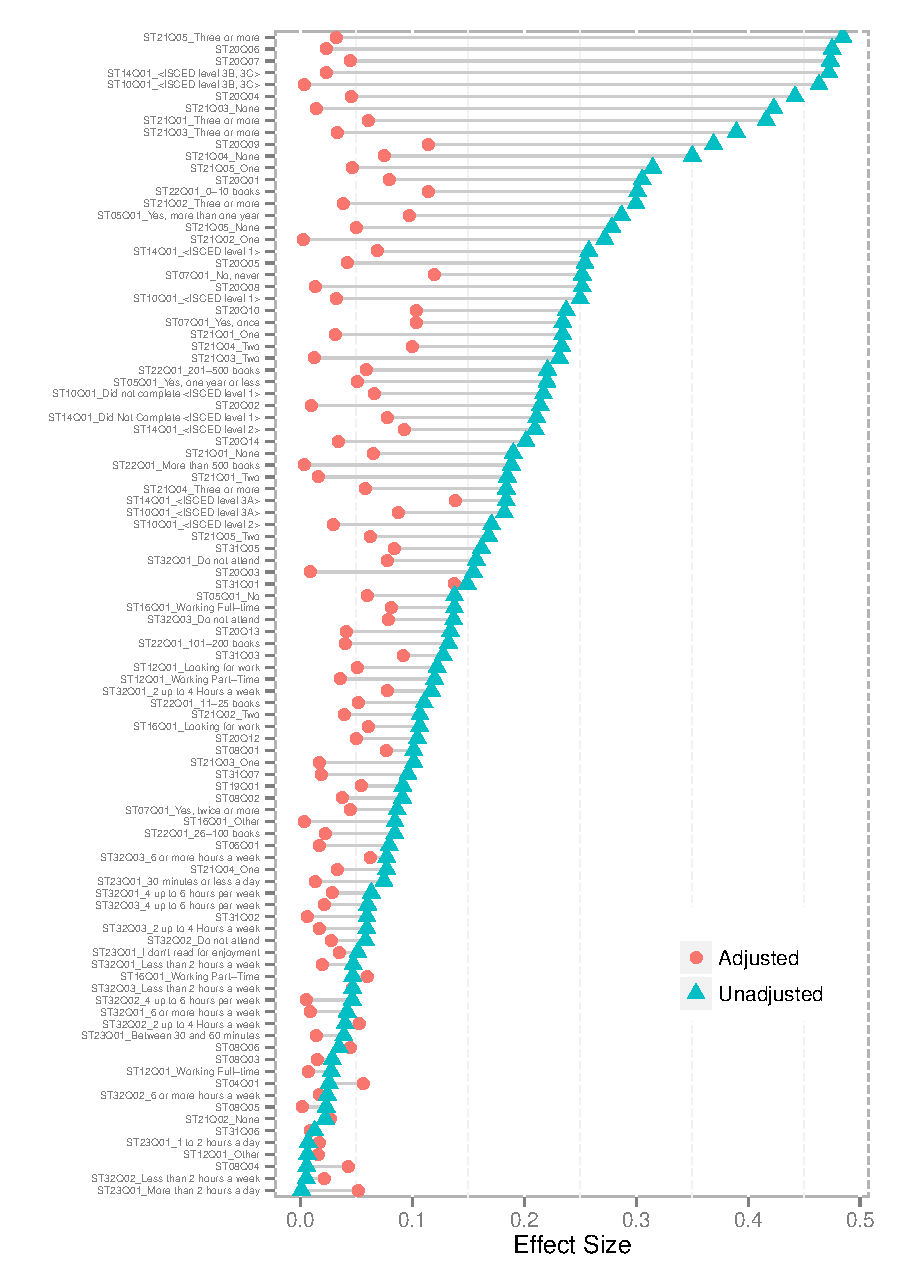
\includegraphics[width=\textwidth]{../Figures/pisabalance.pdf}
\end{center}
\end{figure}

\clearpage

The \texttt{mlpsa} function performs phase II of propensity score analysis and requires four parameters: the response variable, treatment indicator, strata, and clustering indicator. The \texttt{minN} parameter (which defaults to five) indicates what the minimum strata size is to be included in the analysis. For this example, 463, or less than one percent of students were removed because the strata (or leaf node for classification trees) did not contain at least five students from both the treatment and control groups.

\begin{verbatim}
> results.psa.math <- mlpsa(response=mlpsa.df$MathScore, 
                            treatment=mlpsa.df$PUBPRIV, 
                            strata=mlpsa.df$strata, 
                            level2=mlpsa.df$CNT)
Removed 463 (0.696%) rows due to strata size being less than 5
\end{verbatim}

\noindent The \texttt{summary} function provides the overall treatment estimates as well as level one and two summaries.

\begin{verbatim}
> summary(results.psa.math)
Multilevel PSA Model of 85 strata for 3 levels.
Approx t: -10.8
Confidence Interval: -31.3, -24.75
   level2  strata Treat Treat.n Control Control.n ci.min ci.max
1     CAN Overall   579    1625     513     21093  -72.1 -59.57
2    <NA>       1   580      28     492      1128     NA     NA
3    <NA>       2   600       9     476      1326     NA     NA
... # Output truncated to save space
\end{verbatim}

\noindent The \texttt{plot} function will create the multilevel assessment plot. Here it is depicted with side panels showing the distribution of math scores for all strata for public school students to the left and private school students below. These panels can be plotted separately using the \texttt{mlpsa.circ.plot} and \texttt{mlpsa.distribution.plot} functions.

\begin{verbatim}
> plot(results.psa.math)
\end{verbatim}

\begin{figure}[h!]
\begin{center}
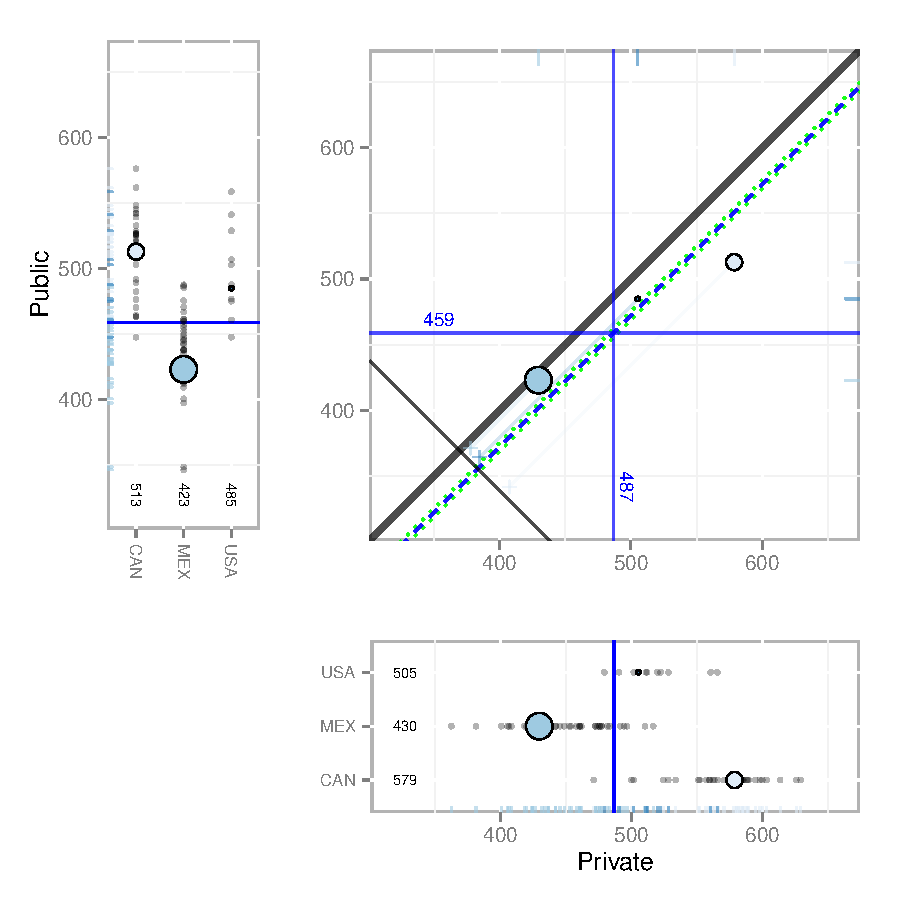
\includegraphics[width=\textwidth]{../Figures/pisamlpsa.pdf}
\end{center}
\end{figure}

\clearpage
Lastly, the \texttt{mlpsa.difference.plot} function plots the overall differences. The \texttt{sd} parameter is optional, but if specified, the \textit{x}-axis can be interpreted as effect sizes.

\begin{verbatim}
> mlpsa.difference.plot(results.psa.math, 
                        sd=mean(mlpsa.df$MathScore, na.rm=TRUE))
\end{verbatim}

\begin{figure}[h!]
\begin{center}
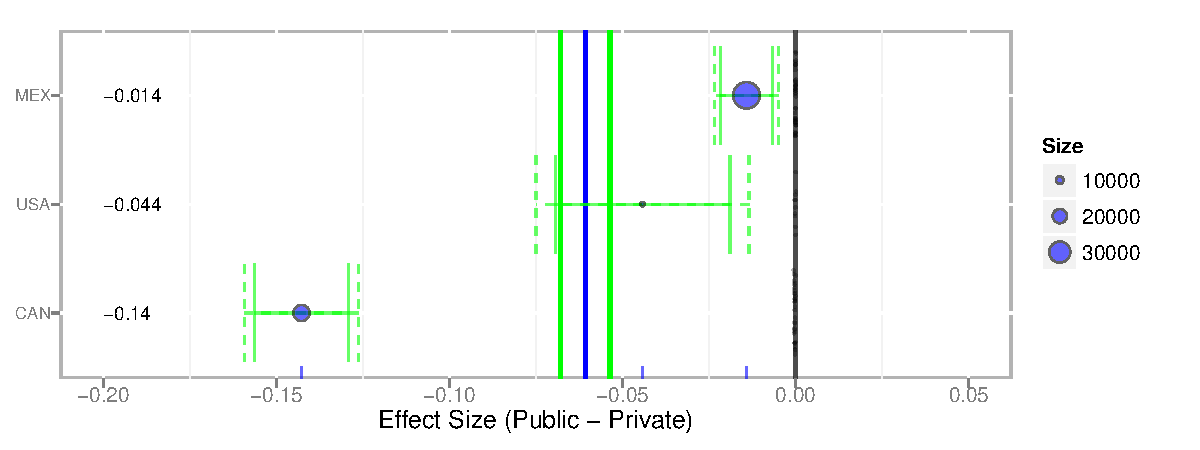
\includegraphics[width=\textwidth]{../Figures/pisadiffplot.pdf}
\end{center}
\end{figure}

\subsection{State Charter Laws and Charter School Performance}

Due to the explicit adjustment within clusters in multilevel PSA, a natural means of comparing clusters is available. That is, since effect sizes are estimated for each cluster, clusters can be compared on those estimated effect sizes. That is, in the process of estimating a national effect size, an effect size for each individual state is also estimated. As such, states can be ranked with regard to the effectiveness of charter school performance within that state.

\citeA{BraunJenkinsGrigg2006} suggested that policies accounted for some of the variation in mean school performance. And indeed, there is wide variability in policies that govern the operation of charter schools from state-to-state, but also within state. The National Alliance for Public Charter Schools (NAPCS) publishes annually rankings of state charter school laws \cite{NAPCS2012}. They argue that some of the performance of charter schools in some states may be hindered by state law. This study will compare the rankings from the multilevel PSA with the state charter school rankings of NAPCS. Slopegraphs \cite{Tufte2001} are a table graphic where two or more columns of data are linked. In this case, rankings from the multilevel PSA with state charter law rankings constitute the two variables to be compared. Each state from each column is connected with a line. This simple graphic can reveal whether there is a relationship between state charter laws and charter school performance in NAEP.


%==================== CHAPTER 4 ====================================================================
\cleardoublepage
\section{Chapter 4: Results}

This chapter will outline in detail the results of all the propensity score models described in chapter three. Since NAEP is organized such that each grade and subject combination is a separate dataset, this chapter will focus on the analysis of grade four math. The results for grade four reading, grade eight math, and grade eight reading are included in the appendices. The chapter begins with details of the nine propensity score methods used and concludes with a summary, including tables and figures, of the overall results across all grades and subjects.

\subsection{Propensity Score Analysis with Stratification}

The first class of propensity score methods used was stratification. The general approach of stratification methods is to subdivide the available sample into smaller groups that have similar covariate profiles. Then a comparison using mean differences between the treatment and control are made, and an overall result is pooled from those individual comparisons. There are several ways to stratify the sample: for this study deciles based upon the propensity scores (i.e. fitted values of a logistic regression model) and leaves of a fitted classification tree were used. Moreover, given the importance of covariate selection and omission from propensity score models, two types of logistic regression models were used, namely a full model using all available covariates and an Akaike Information Criterion \cite<AIC;>{Akaike1974} optimized model. The former is determined by a stepwise model selection algorithm where covariates are added and dropped and the model that optimizes the AIC is retained. Like all analysis in phase one, this was done without outcome variables.

\begin{figure}[t]
\begin{center}
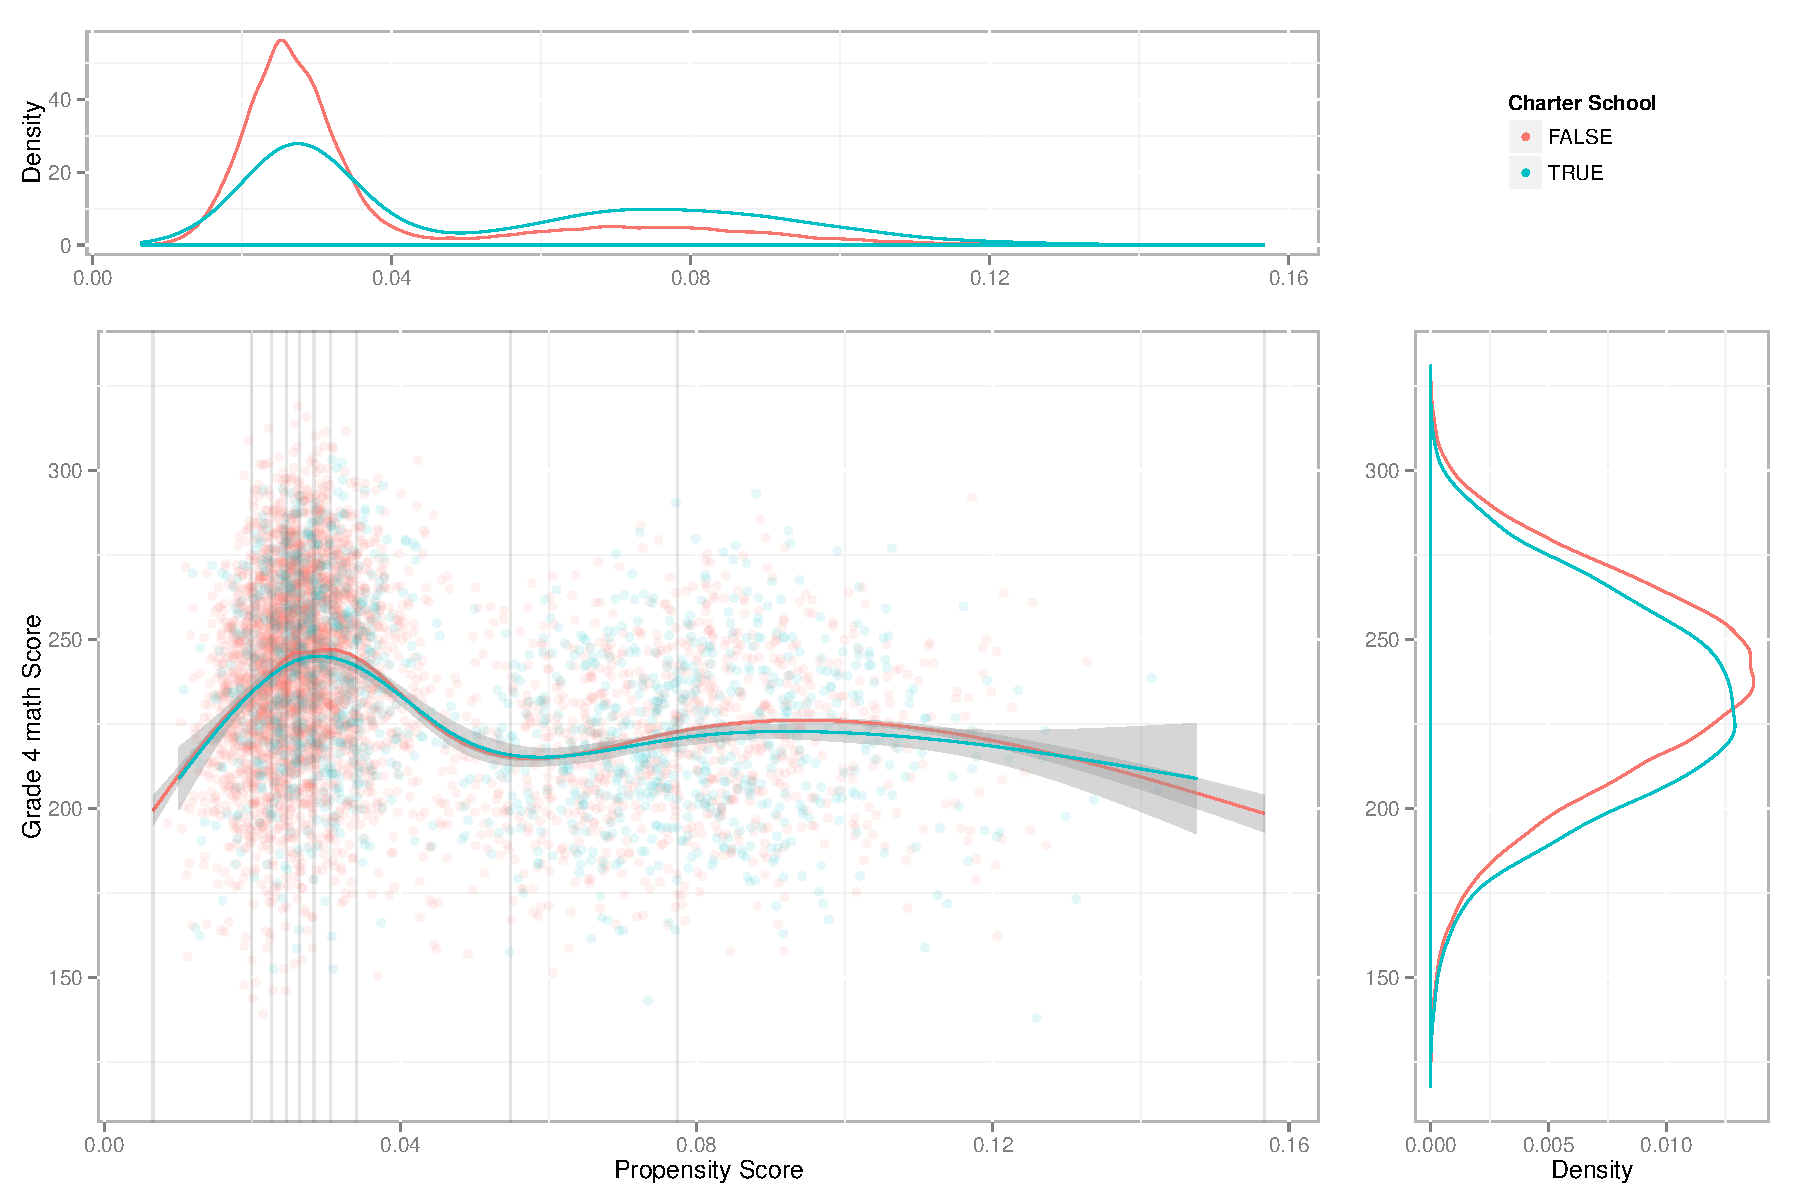
\includegraphics[width=\textwidth]{../Figures2009/g4math-loess.pdf}
\caption{Loess regression assessment plot: Grade 4 math}
\label{fig:g4math:loess}
\end{center}
\end{figure}

However, before stratifying the logistic regression models, I examined the relationship between propensity scores and the outcome variable for the two groups and fitted a Loess regression line to the scatter plot to provide an overall indication of the differences, if any. Figure \ref{fig:g4math:loess} is a Loess Regression Assessment Plot created using the loess.plot function in the \texttt{multilevelPSA} package. The main panel is a scatterplot of each student's propensity score on the \textit{x}-axis and math score on the \textit{y}-axis (for clarity a random 10\% sample of data points are plotted; more than 10\% would have resulted in a graphic too dense to interpret). 

Two fitted Loess regression lines with approximate 95\% confidence intervals are also plotted. Loess lines are based upon the full dataset. The panel on the top provides density distributions of the propensity scores and shows that there is generally good overlap between the two groups. Having adequate overlap is critical since it indicates there are treatment and comparison units with similar propensity scores that will be compared on their outcome variables. The panel on the right is a density distribution of the unadjusted outcome and shows that before propensity score adjustment, traditional public school students performed slightly better than charter school students. However, given the strong overlap in the two Loess regression lines, this figure suggests there is no discernible difference in performance between traditional public school students and charter school students in grade four math. Corresponding plots for the other datasets, as well as those for the AIC optimized models, are provided in Appendix D.

The vertical lines in the main panel of Figure \ref{fig:g4math:loess} represent the deciles, or strata. Figure \ref{fig:g4math:circpsa} is a propensity score assessment plot where the \textit{x}-axis is the outcome score for charter schools and the \textit{y}-axis is the outcome score for traditional public schools. Each circle corresponds to each strata and the size of the circle is proportional to the number of students within each strata. For the Logistic regression models, since deciles were used, each circle is of the same size. Figure \ref{fig:g4math:circpsa:tree} is the corresponding propensity score assessment plot for the classification tree model and therefore each strata is not of the same size. Points that lie on or near the unit line, $y = x$, indicate no significant difference in the outcome of the two scores. Lines are projected to a line perpendicular to the unit line and the tick placed. These tick marks correspond to the distribution of difference scores and the dashed blue line parallel to the unit line the overall mean difference. Furthermore, the green bar represents exactly the 95\% confidence interval. The fact that the confidence interval does not span the unit line and is on the tradition public school side indicates there is a small, statistically significant difference in favor of traditional public school students. Tables \ref{g4math-circpsa10}, \ref{g4math-circpsa10AIC}, and \ref{g4math-circpsa-tree} provide numeric results for each strata. Appendix F contains propensity score assessment plots and summary tables for grade four reading, grade eight math, and grade eight reading.

\begin{figure}[t]
\begin{center}
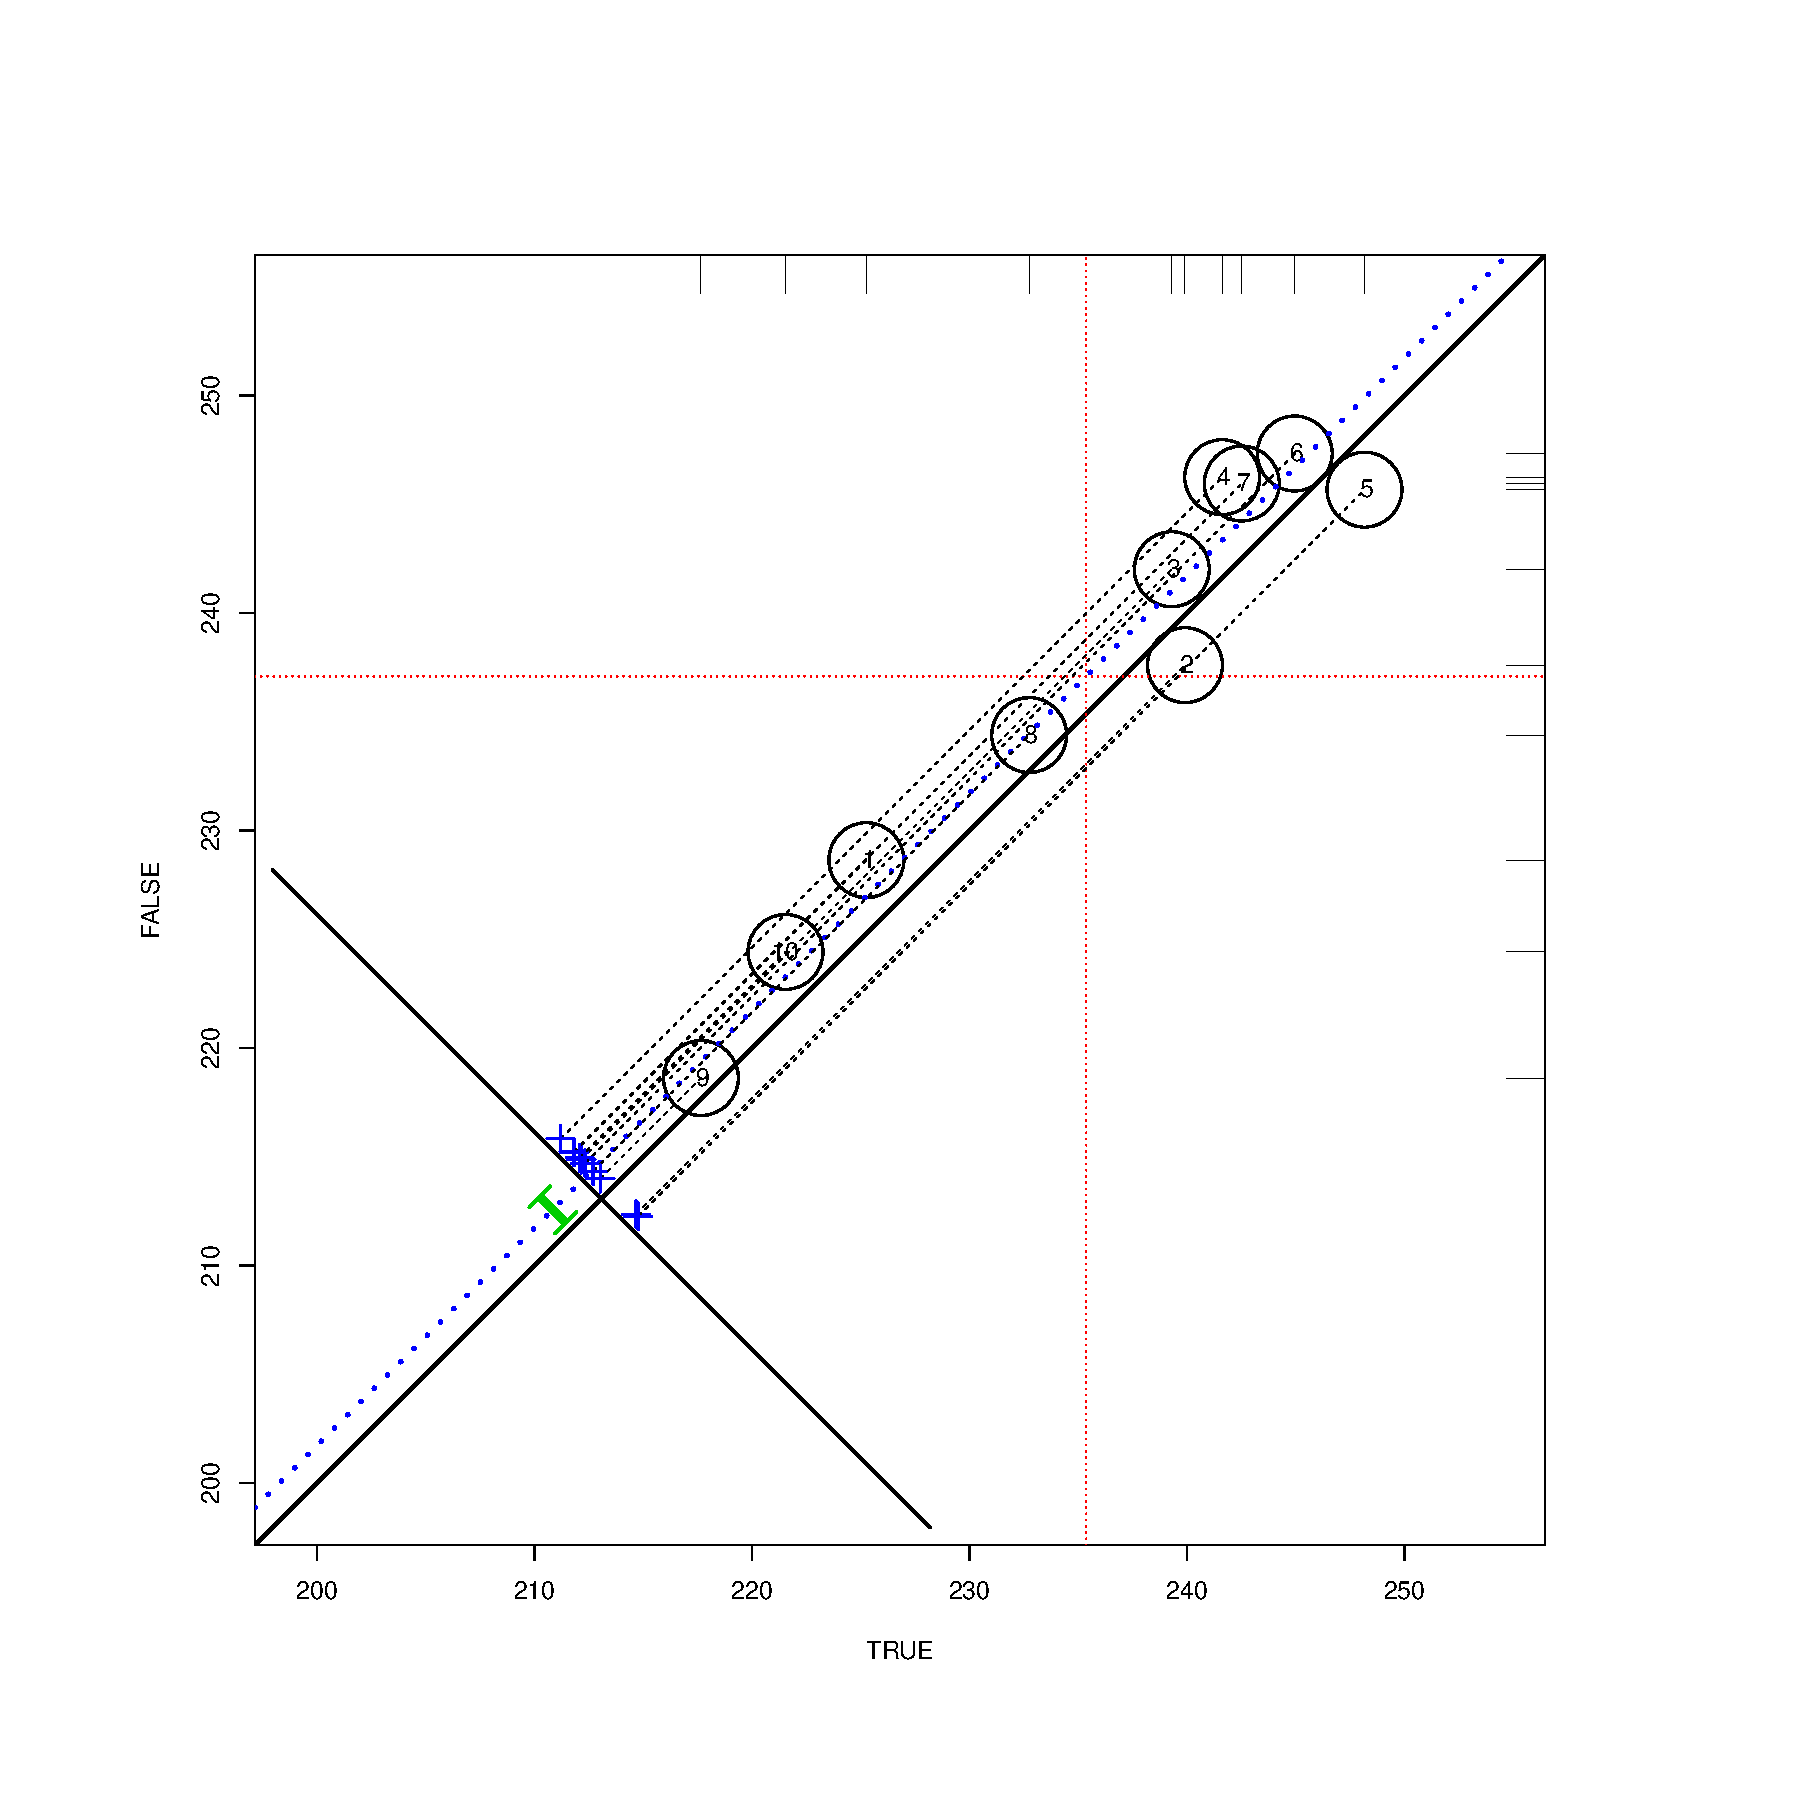
\includegraphics[width=\textwidth]{../Figures2009/g4math-circpsa10.pdf}
\caption{Propensity score assessment plot for logistic regression stratification: Grade 4 math}
\label{fig:g4math:circpsa}
\end{center}
\end{figure}

\begin{figure}[t]
\begin{center}
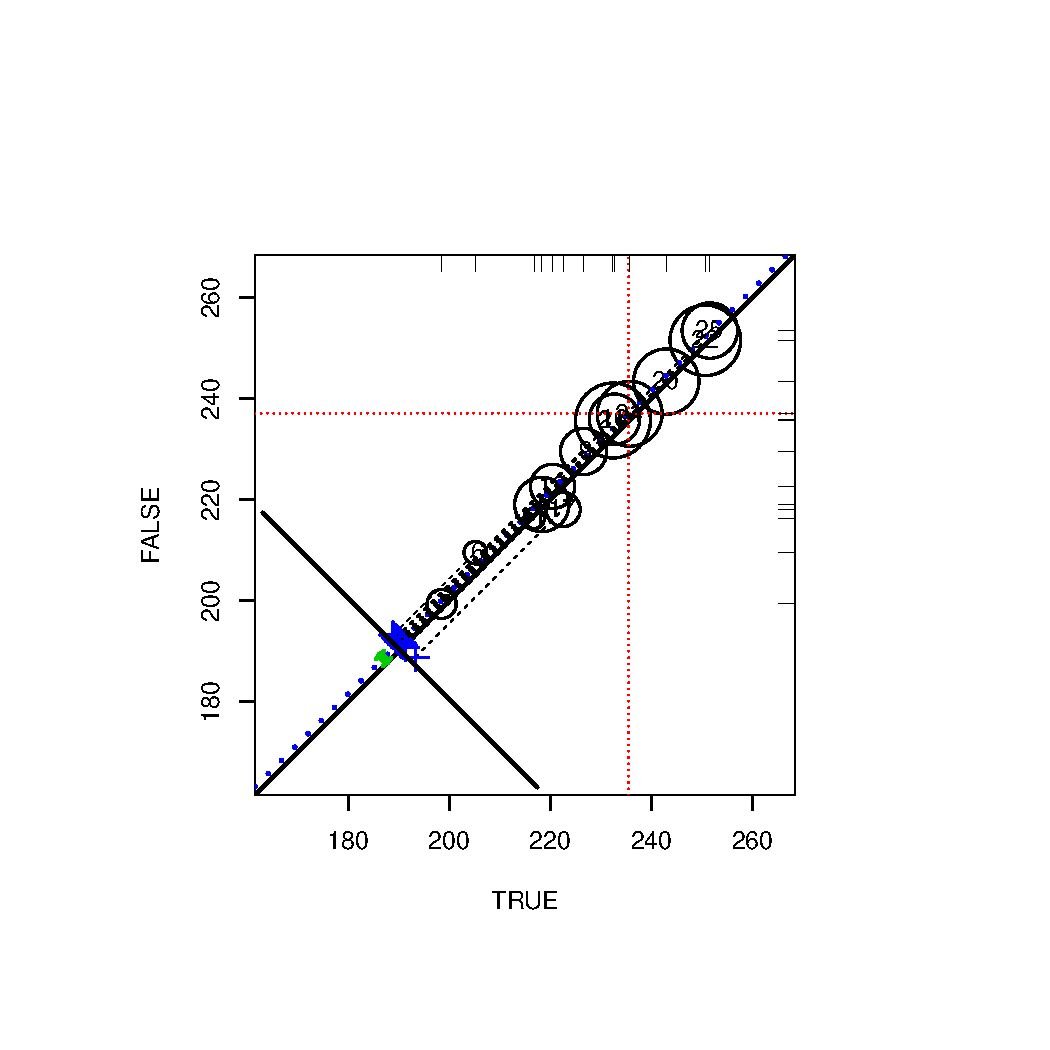
\includegraphics[width=\textwidth]{../Figures2009/g4math-circpsa-tree.pdf}
\caption{Propensity score assessment plot for classification tree stratification: Grade 4 math}
\label{fig:g4math:circpsa:tree}
\end{center}
\end{figure}

\subsubsection{Covariate Balance}

The goal of propensity score methods is to adjust for selection bias with the available observed covariates, and the results discussed above are only as good as the balance achieved. In practice we test for the effectiveness of bias reduction by evaluating covariate balance. Perfect balance is achieved when there are no differences in covariate values for any matched pair or strata. However, perfect balance is almost never achieved. Figure \ref{fig:g4math:balance} is a Covariate Effect Size balance plot. For each covariate on the \textit{y}-axis, the absolute standardized effect size before adjustment (in red) and after adjustment (in blue) are plotted. Effect sizes for individual strata are represented by letters. This figure shows that the propensity score adjustment greatly reduced the effects of each covariate. There is not a conventional adjusted effect size threshold for achieving sufficient balance in the PSA literature. However, more generally \citeA{Cohen1988} has suggested that an effect size between 0.2 and 0.3 would be small. As a general rule of thumb I suggest that an adjusted effect size of less than 0.1 would be very small (accounting for less than 1\% of the variance in the model) and therefore evidence of sufficient balance. The remaining covariate balance plots are provided in Appendix E.

% latex table generated in R 3.0.2 by xtable 1.7-1 package
% Sun Feb 23 12:15:58 2014
\begin{table}[ht]
\centering
\caption{Logistic Regression Stratification Results for Grade 4 math} 
\label{g4math-circpsa10}
\begin{tabular}{lrr@{\extracolsep{.2cm}}rr}
  \hline
   & \multicolumn{2}{c}{Public} & \multicolumn{2}{c}{Charter} \\ \cline{2-3} \cline{4-5} Strata & Mean & n & Mean & n \\ \hline
1 & 228.64 & 8702 & 225.26 & 158 \\ 
  2 & 237.61 & 8694 & 239.91 & 165 \\ 
  3 & 242.02 & 8637 & 239.31 & 222 \\ 
  4 & 246.25 & 8645 & 241.62 & 214 \\ 
  5 & 245.68 & 8607 & 248.17 & 253 \\ 
  6 & 247.34 & 8615 & 244.96 & 244 \\ 
  7 & 245.96 & 8566 & 242.53 & 293 \\ 
  8 & 234.39 & 8494 & 232.75 & 365 \\ 
  9 & 218.62 & 8246 & 217.66 & 613 \\ 
  10 & 224.42 & 8066 & 221.55 & 794 \\ 
   \hline
\end{tabular}
\end{table}


\begin{figure}[t]
\begin{center}
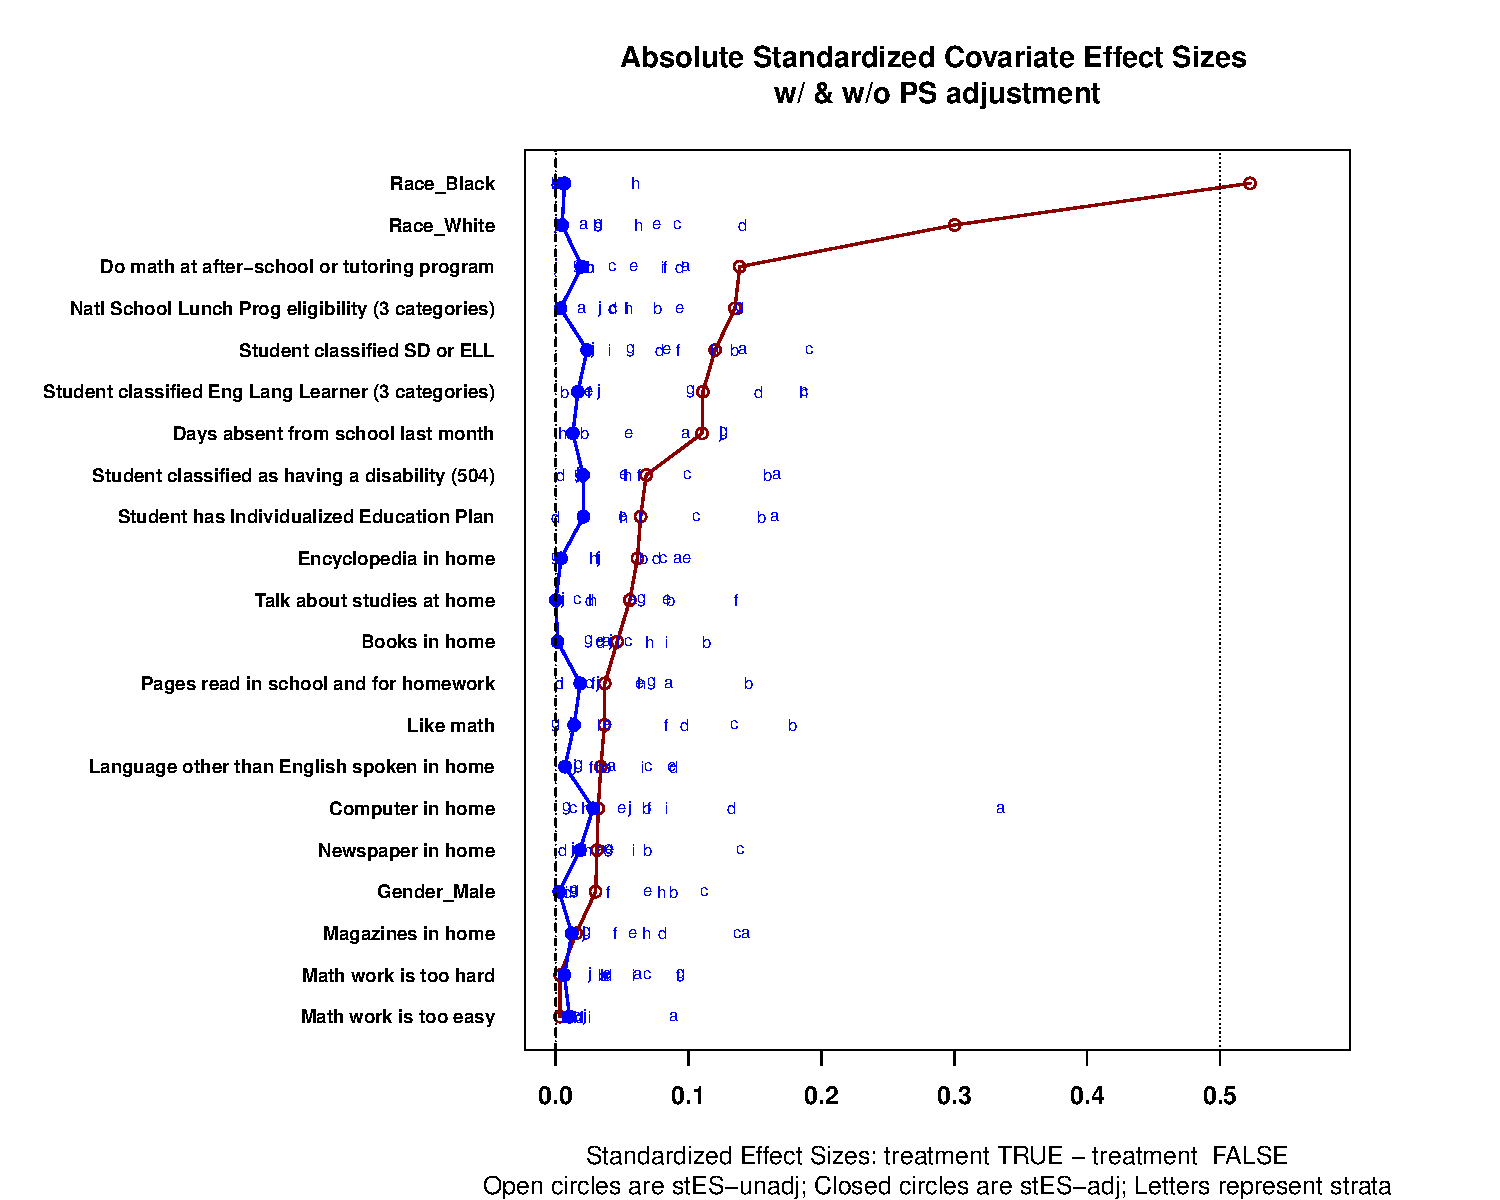
\includegraphics[width=\textwidth]{../Figures2009/g4math-lr-balance.pdf}
\caption{Covariate balance plot for logistic regression stratification: Grade 4 math}
\label{fig:g4math:balance}
\end{center}
\end{figure}


\clearpage
% latex table generated in R 3.0.2 by xtable 1.7-1 package
% Sun Feb 23 12:15:58 2014
\begin{table}[ht]
\centering
\caption{Logistic regression AIC stratification results for grade 4 math} 
\label{g4math-circpsa10AIC}
\begin{tabular}{lrr@{\extracolsep{.2cm}}rr}
  \hline
   & \multicolumn{2}{c}{Public} & \multicolumn{2}{c}{Charter} \\ \cline{2-3} \cline{4-5} Strata & Mean & n & Mean & n \\ \hline
1 & 229.81 & 8864 & 226.26 & 165 \\ 
  2 & 239.11 & 8630 & 241.24 & 162 \\ 
  3 & 245.14 & 11091 & 243.45 & 275 \\ 
  4 & 244.90 & 6095 & 242.28 & 160 \\ 
  5 & 244.90 & 8719 & 244.52 & 262 \\ 
  6 & 246.66 & 8483 & 246.44 & 250 \\ 
  7 & 245.45 & 8581 & 241.09 & 291 \\ 
  8 & 232.05 & 8507 & 231.18 & 349 \\ 
  9 & 218.70 & 8331 & 217.03 & 621 \\ 
  10 & 224.41 & 7971 & 222.01 & 786 \\ 
   \hline
\end{tabular}
\end{table}

% latex table generated in R 3.0.2 by xtable 1.7-1 package
% Sun Feb 23 12:15:58 2014
\begin{table}[ht]
\centering
\caption{Classification trees stratification results for grade 4 math} 
\label{g4math-circpsa-tree}
\begin{tabular}{lrr@{\extracolsep{.2cm}}rr}
  \hline
   & \multicolumn{2}{c}{Public} & \multicolumn{2}{c}{Charter} \\ \cline{2-3} \cline{4-5} Strata & Mean & n & Mean & n \\ \hline
5 & 219.03 & 6783 & 218.32 & 492 \\ 
  6 & 209.53 & 731 & 205.16 &  78 \\ 
  7 & 199.37 & 1469 & 198.49 &  68 \\ 
  9 & 229.54 & 4489 & 226.60 & 376 \\ 
  11 & 216.31 & 595 & 216.81 &  38 \\ 
  12 & 222.64 & 3920 & 220.45 & 438 \\ 
  16 & 235.93 & 5918 & 232.69 & 110 \\ 
  17 & 218.06 & 2272 & 222.53 &  69 \\ 
  20 & 243.38 & 11290 & 242.95 & 260 \\ 
  21 & 235.67 & 15740 & 232.40 & 487 \\ 
  22 & 251.54 & 13499 & 250.68 & 478 \\ 
  24 & 237.01 & 11130 & 235.71 & 223 \\ 
  25 & 253.48 & 7436 & 251.58 & 204 \\ 
   \hline
\end{tabular}
\end{table}



\subsection{Propensity Score Matching}

The second class of propensity score method used is propensity score matching. In propensity score matching, the goal is to match students from the two groups with small differences in their propensity scores in order to adjust for selection bias. In large datasets, or when particular covariates are determined to be more important for adjusting selection bias, whether theoretically or otherwise, partial exact matching is done. In the context of this study, partial exact matching is akin to implicitly adjusting for the multilevel nature of the data. Students were first matched exactly by state, gender, and ethnicity, and then by propensity score using nearest neighbor (i.e. the difference between propensity scores of pairs is minimized). Propensity scores from the full logistic regression model were used for matching.

The \texttt{Matchby} function in the \texttt{Matching} package \cite{matching} was used to find matches. First, propensity scores were estimated using the full logistic regression model. The \texttt{Matchby} algorithm first determines which students match exactly on state, gender, and ethnicity. Within those subgroups, students with the smallest standardized difference and less than 0.25 standard deviations, are returned. Three matched sets were produced (stated as charter-to-public): one-to-one, one-to-five, and one-to-ten. Matching was done without replacement.

Once matched pairs were determined, dependent sample \textit{t}-tests were performed \cite{Austin2011} to estimate average treatment effect and corresponding confidence intervals. Figures \ref{fig:overallcirc} and \ref{fig:overalldiff} and Table \ref{tab:overall} at the end of the chapter provide the overall results. In general however, matching methods tend to estimate slightly larger treatment effects than both the stratification and multilevel models. And of additional note, the confidence intervals shrink as the ratio of treatment-to-control units increase.


\subsection{Multilevel Propensity Score Analysis}

The final class of propensity score method utilized in multilevel propensity score analysis. This approach to PSA was developed for this dissertation and implemented in the \texttt{multilevelPSA} R package. The multilevel PSA approach makes explicit in both phase I and II the multilevel nature of the data, in the case of this study, state. In principle, the multilevel PSA approach is a conceptual combination of the partial exact matching and stratification. However, whereas partial exact matching utilizes propensity scores estimated from a single logistic regression model, the multilevel PSA algorithm will estimate separate propensity score models, using either logistic regression or classification trees (both were done for this study), for each level two cluster (i.e. state). That is, the algorithm will perform \textit{m} separate propensity score analyses using stratification where \textit{m} is the number of states. This approach provides average treatment effects for each state as well as an overall, national, estimated treatment effect.

\begin{figure}[t]
\begin{center}
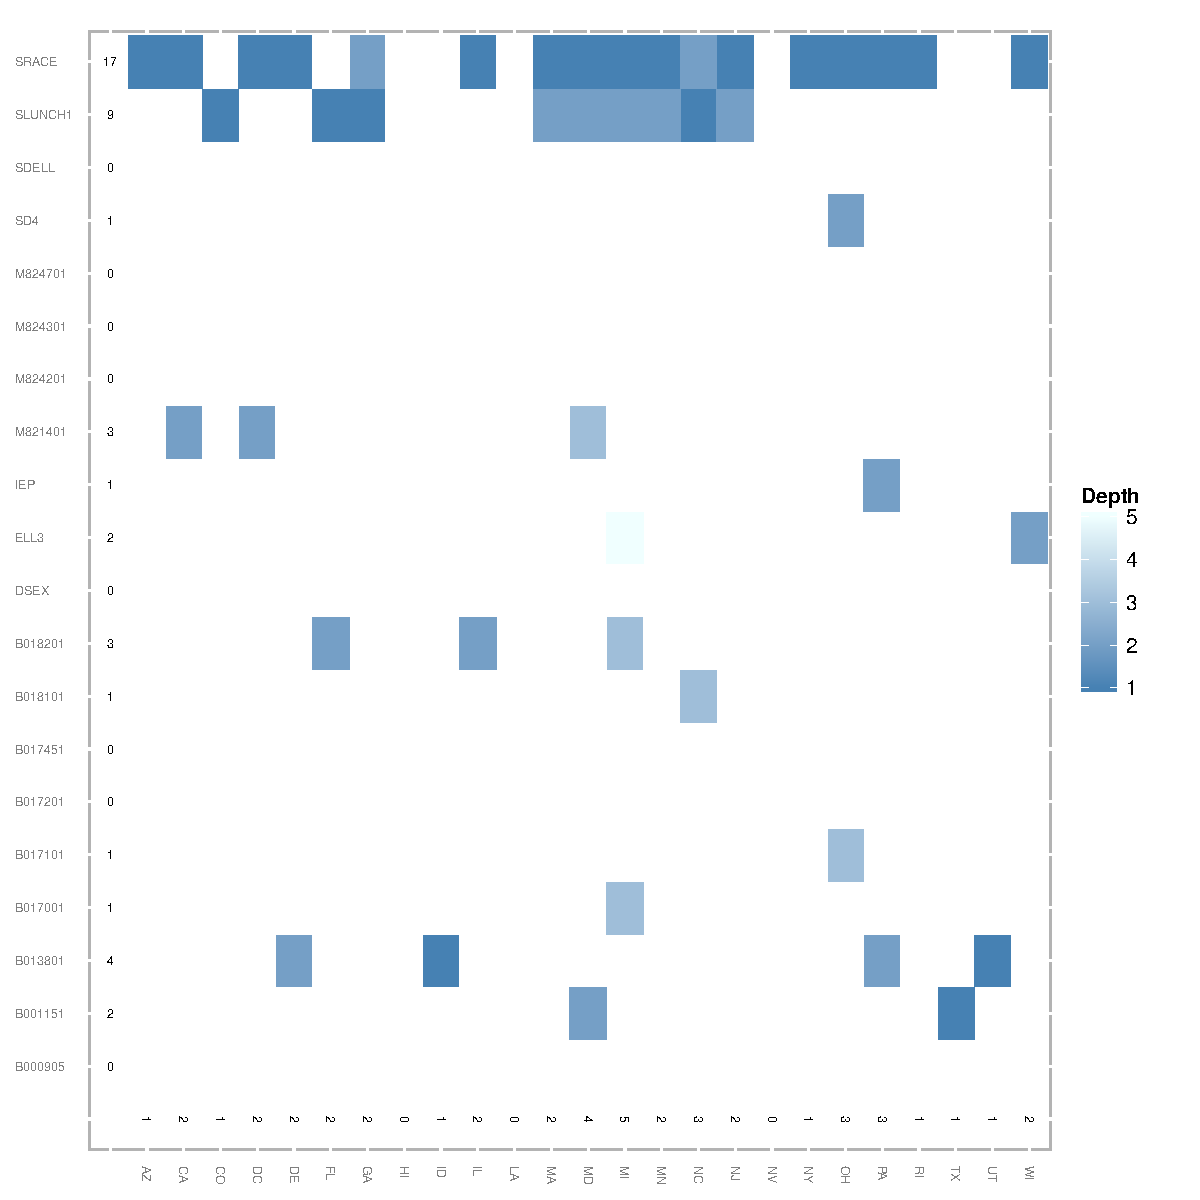
\includegraphics[width=\textwidth]{../Figures2009/g4math-mlpsa-ctree-heat.pdf}
\caption{Multilevel PSA covariate heat map for classification trees: Grade 4 math}
\label{fig:g4math-mlpsa-ctree-heat}
\end{center}
\end{figure}

The same three methods of stratification described above were used: full logistic regression model using all covariates, logistic regression model that optimized Akaike Information Criterion (AIC), and classification trees. For the logistic regression models strata are defined using quintiles of the propensity scores. One difficulty in interpreting results for multilevel PSA models is the relative importance of covariates for predicting treatment. Figure \ref{fig:g4math-mlpsa-ctree-heat} is a covariate heat map that depicts each covariate on the \textit{y}-axis and state on the \textit{x}-axis. If a covariate is present in the fitted classification tree for that state, the intersecting cell is shaded. The darkness of the color represents how far down the tree that covariate first appears. That is, the darkest color indicates that the covariate was used to split the tree at the root (or the first splitting covariate). This provides an opportunity to compare the relative importance of each covariate across states. The results for grade four math show that ethnicity is the strongest predictor of treatment, having appeared in 17 of the trees, with National School Lunch eligibility as the second. For the classification tree methods, strata with fewer than five students in either of the two groups were eliminated. Since quintiles were used for the logistic regression models, all students within those states are used. Table \ref{g4math-circpsa10} provides the results within each strata of each state including strata size.

\subsubsection{Covariate Balance}

\begin{figure}[t]
\begin{center}
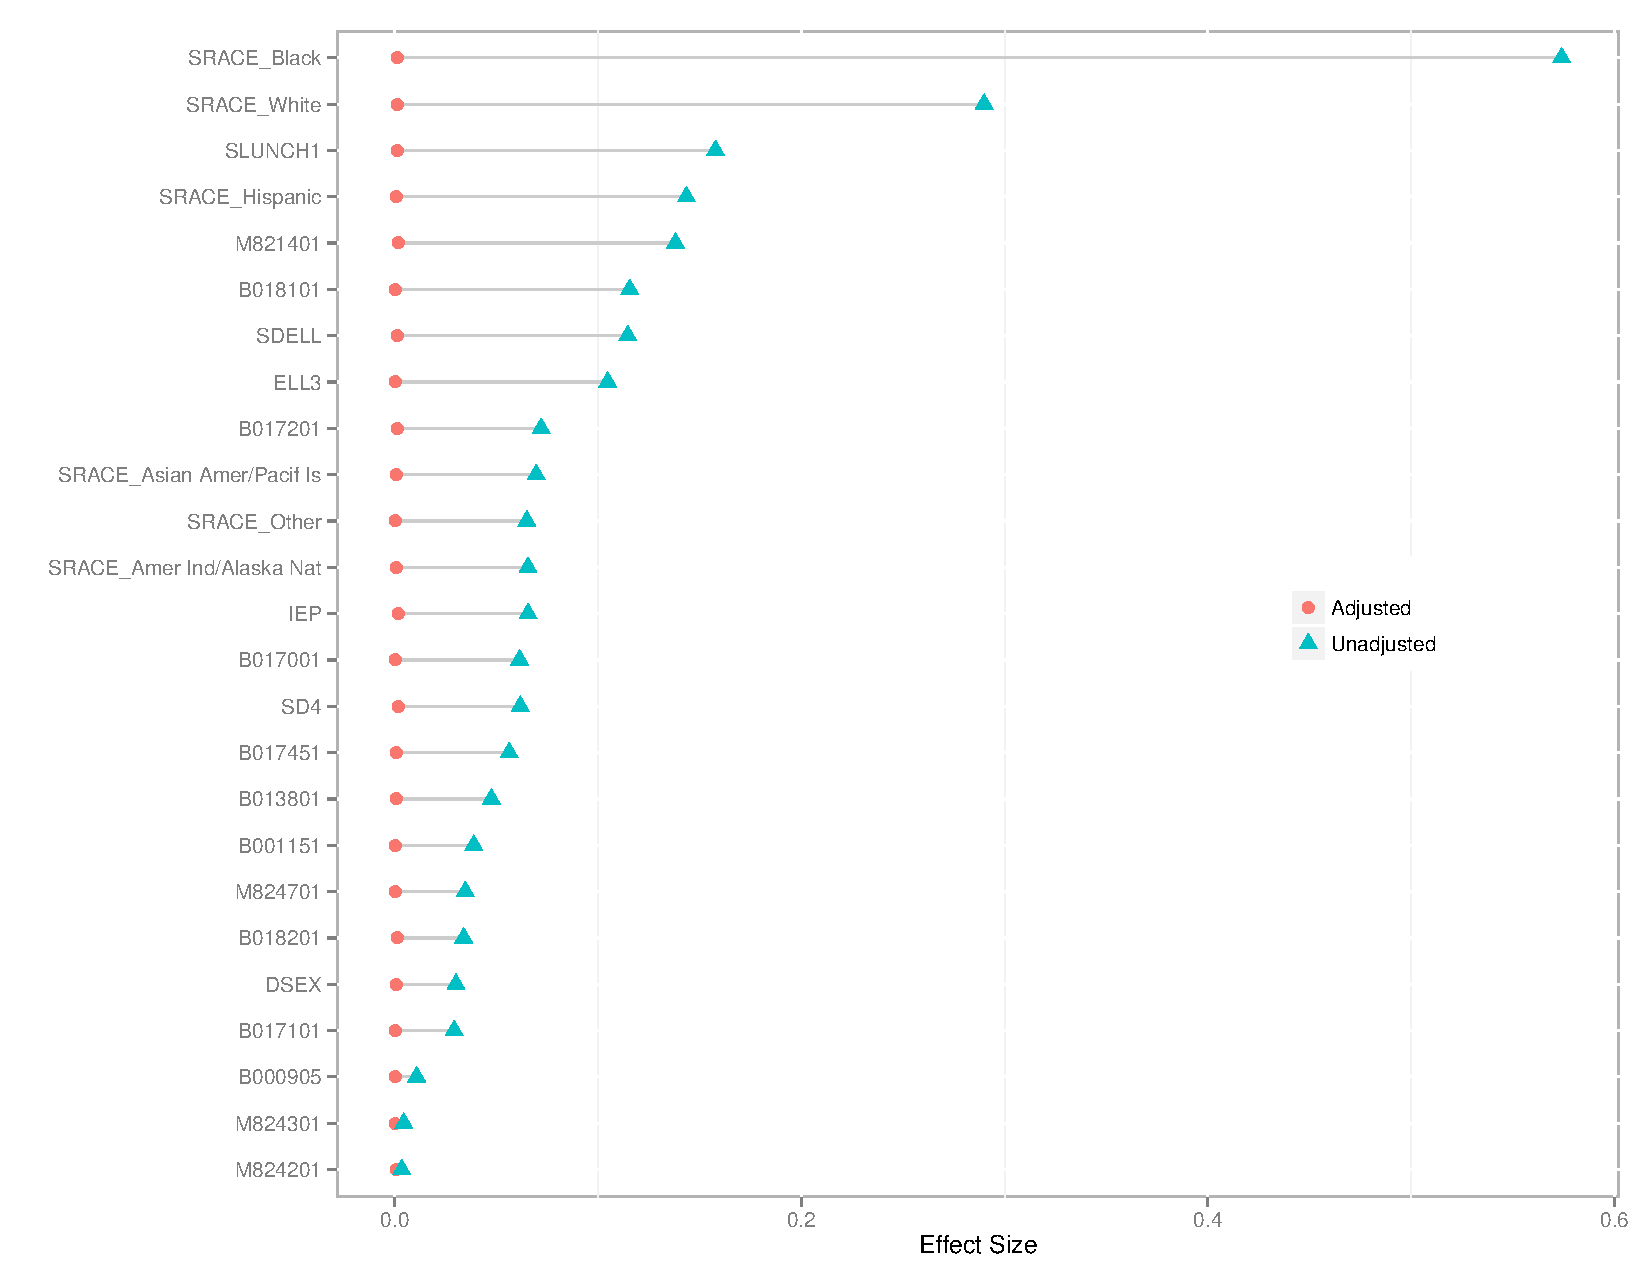
\includegraphics[width=\textwidth]{../Figures2009/g4math-mlpsa-ctree-balance.pdf}
\caption{Multilevel PSA covariate balance plot classification trees: Grade 4 math}
\label{fig:g4math-mlpsa-ctree-balance}
\end{center}
\end{figure}

Figure \ref{fig:g4math-mlpsa-ctree-balance} is the multilevel PSA counterpart to the covariate balance plot described above. Individual strata have been excluded for clarity since there are substantially more strata. This figure shows that, in general, relatively good balance has been achieved since the adjusted absolute effect sizes are smaller or not substantially different than the unadjusted effect sizes, and using the same criteria discussed above, all the adjusted effect sizes are smaller than 0.1. The remaining multilevel PSA covariate balance plots are provided in Appendix G. The classification tree methods, in general, provide much better balance than the logistic regression models. This is a limitation of estimating logistic regression models with samples that have disproportional numbers of control-to-treatment students in the dependent variable. As such, interpreting the multilevel PSA logistic regression models in isolation is discouraged. However, this study follows the advice of \citeA{Rosenbaum2012} in that these are just two of the nine methods used to estimate causal effects.

\subsubsection{Visualizing Multilevel PSA}

An important advantage of multilevel PSA is that average treatment effects can be estimated for each state and then aggregated to provide a national average treatment effect. A number of graphics have been developed to help interpret these results. Figure \ref{fig:g4math-mlpsa-ctree} is a multilevel PSA assessment plot for grade four math. This is an extension of the PSA assessment plots described above. Each point represents the overall adjusted score for each state (the point size is proportional to the number of students sampled in each state) with traditional public schools on the \textit{x}-axis and charter schools on the \textit{y}-axis. The overall national mean scores are represented by the blue lines. The tick marks on the line perpendicular to the unit line ($y = x$) represent the distribution of differences for states. The dashed blue line\footnote{For this dataset the blue and green lines almost completely overlaps the unit line but are present.} is the overall national mean difference and the green lines are the 95\% confidence interval. This figure depicts that there is not a statistically significant difference nationally for grade four math using classification trees as evidenced by the confidence interval (the green lines) overlapping the zero (the unit line). Moreover, there is minimal difference for most states, since most of the points fall close to the unit line. However, there are some states that have a small positive effect size for charter school students  while others have a small negative effect. 

\begin{figure}[t]
\begin{center}
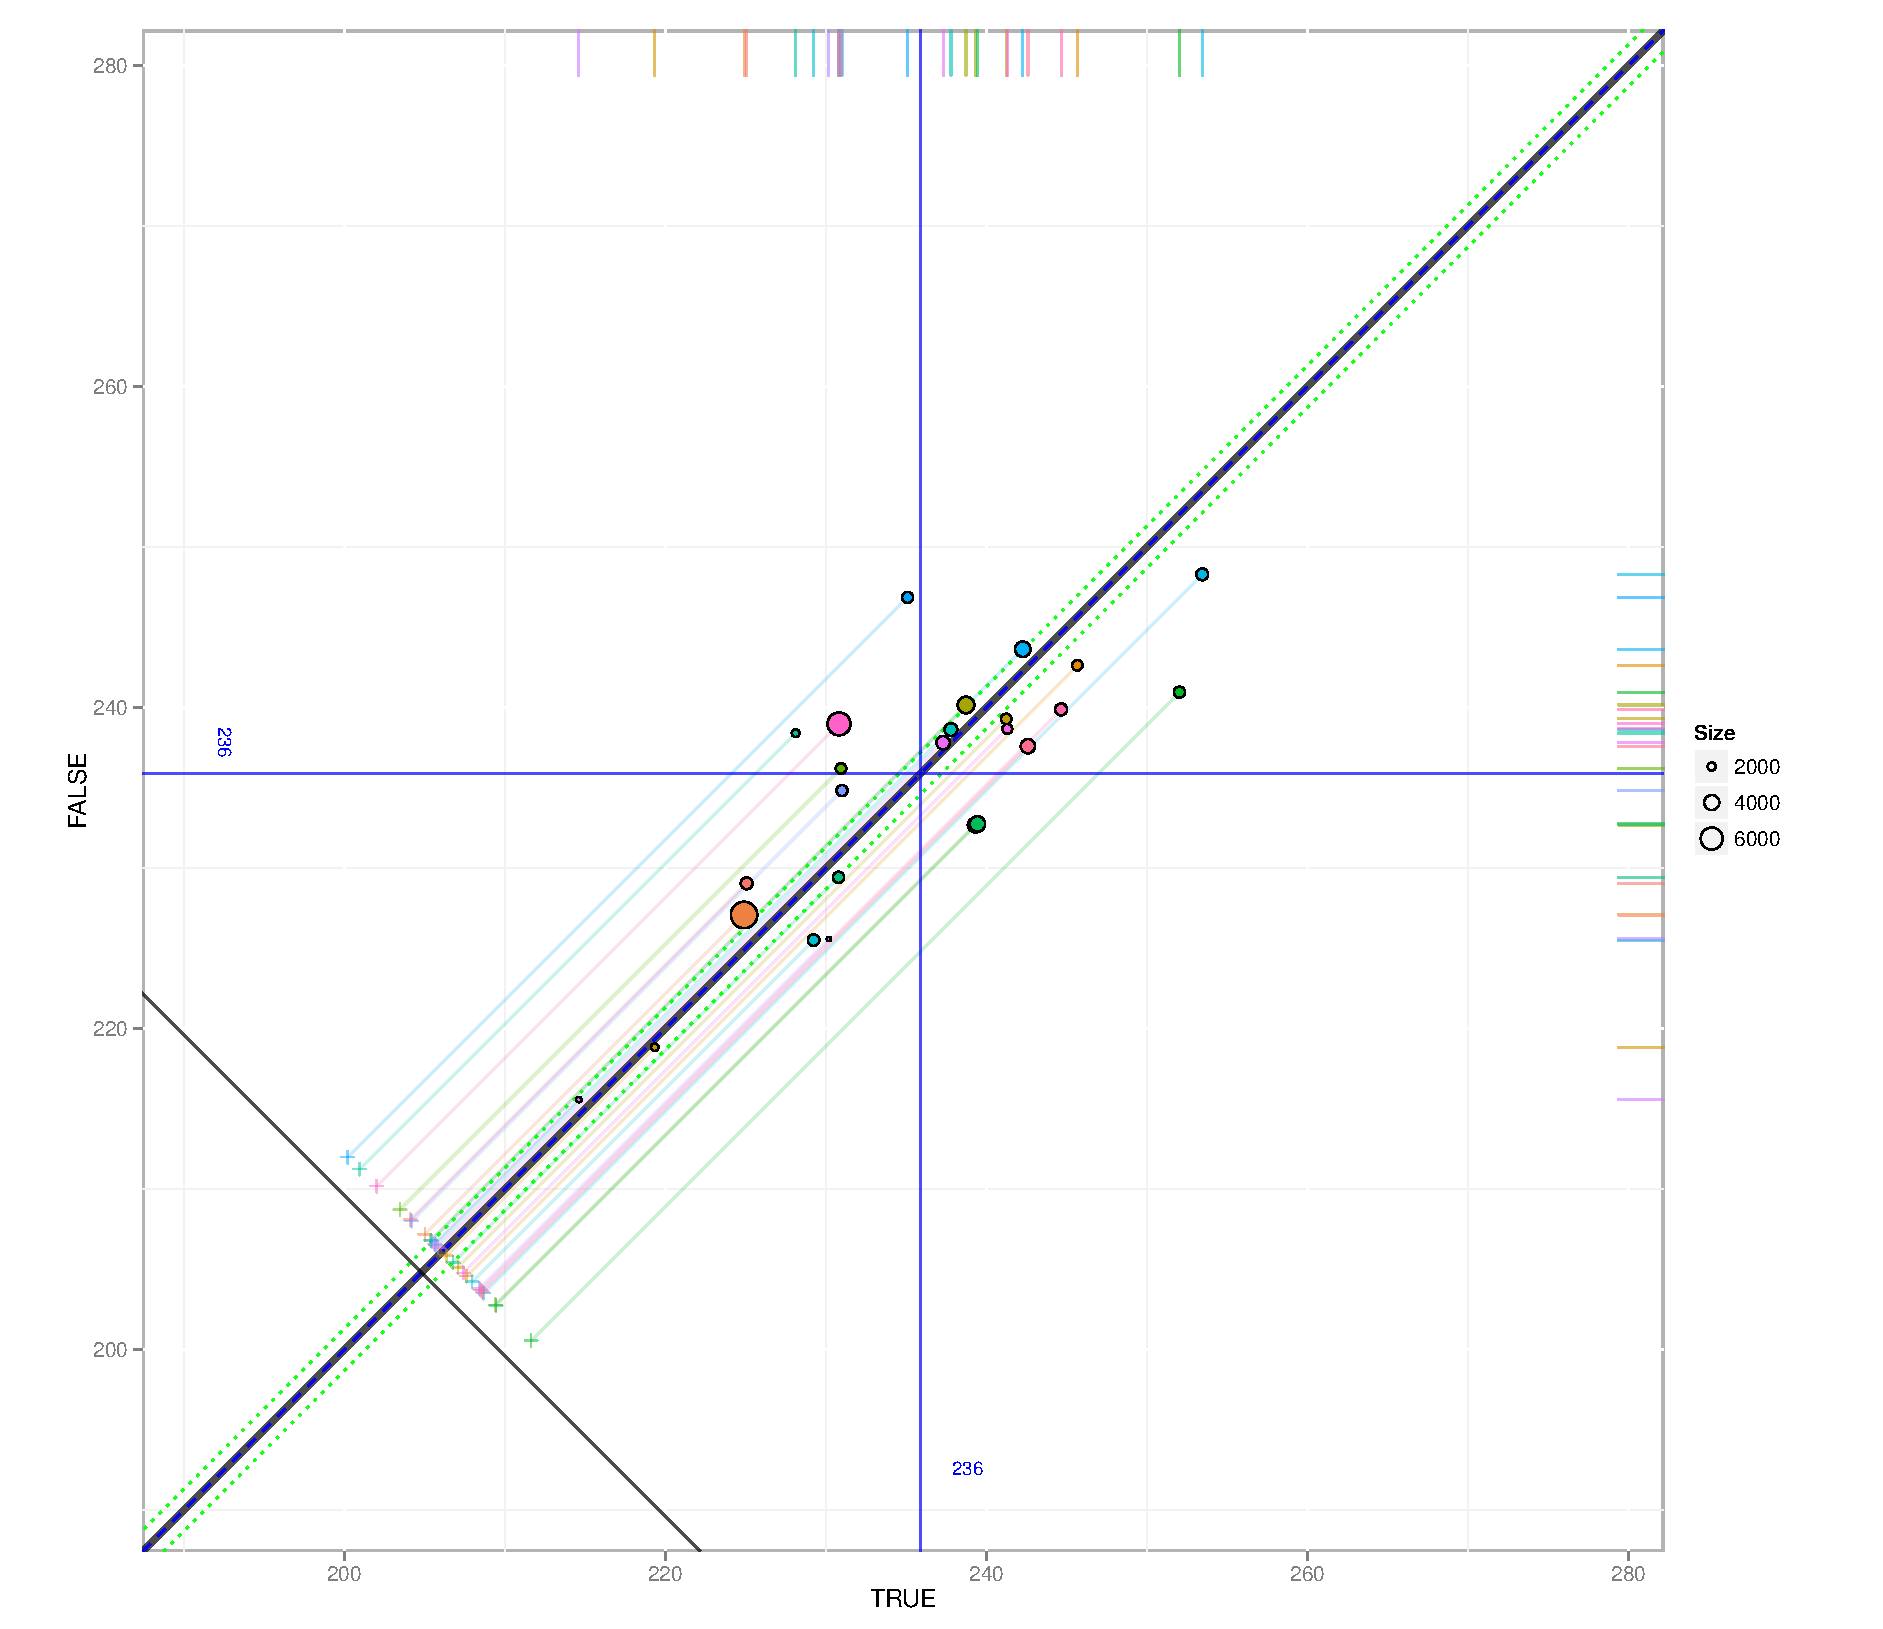
\includegraphics[width=\textwidth]{../Figures2009/g4math-mlpsa-ctree-circ.pdf}
\caption{Multilevel PSA assessment plot classification trees: Grade 4 math}
\label{fig:g4math-mlpsa-ctree}
\end{center}
\end{figure}

Figure \ref{fig:g4math-mlpsa-ctree-diff} provides a more detailed depiction of the differences in Figure \ref{fig:g4math-mlpsa-ctree}. The tick marks in Figure \ref{fig:g4math-mlpsa-ctree} on the line perpendicular to the unit line in the lower left corner of the plot correspond to the distribution of difference scores. Figure \ref{fig:g4math-mlpsa-ctree-diff} represents only this distribution with more details. Specifically, the small grey points correspond to the difference for each strata. The blue points are the overall difference for each state, with the point size corresponding to the number of students sampled. The 95\% confidence intervals for each state are provided in green. The overall adjusted national effect size and corresponding 95\% confidence interval are represented by the vertical blue line and vertical green lines, respectively. From this figure, charter school students performed statistically significantly better than traditional public school students in Idaho, Illinois, Georgia, and Minnesota as evidenced by the confidence intervals that do not span zero. Conversely, charter school students performed lower than traditional public school students in Arizona, Texas, Massachusetts, and New Jersey. For all other states there was no statistical difference. From a national perspective, there is no difference between the performance of charter and traditional public school students as evidenced by the vertical green lines spanning zero. Figures for grade four reading, grade eight math, and grade eight reading are provided in Appendix H.

\begin{figure}[t]
\begin{center}
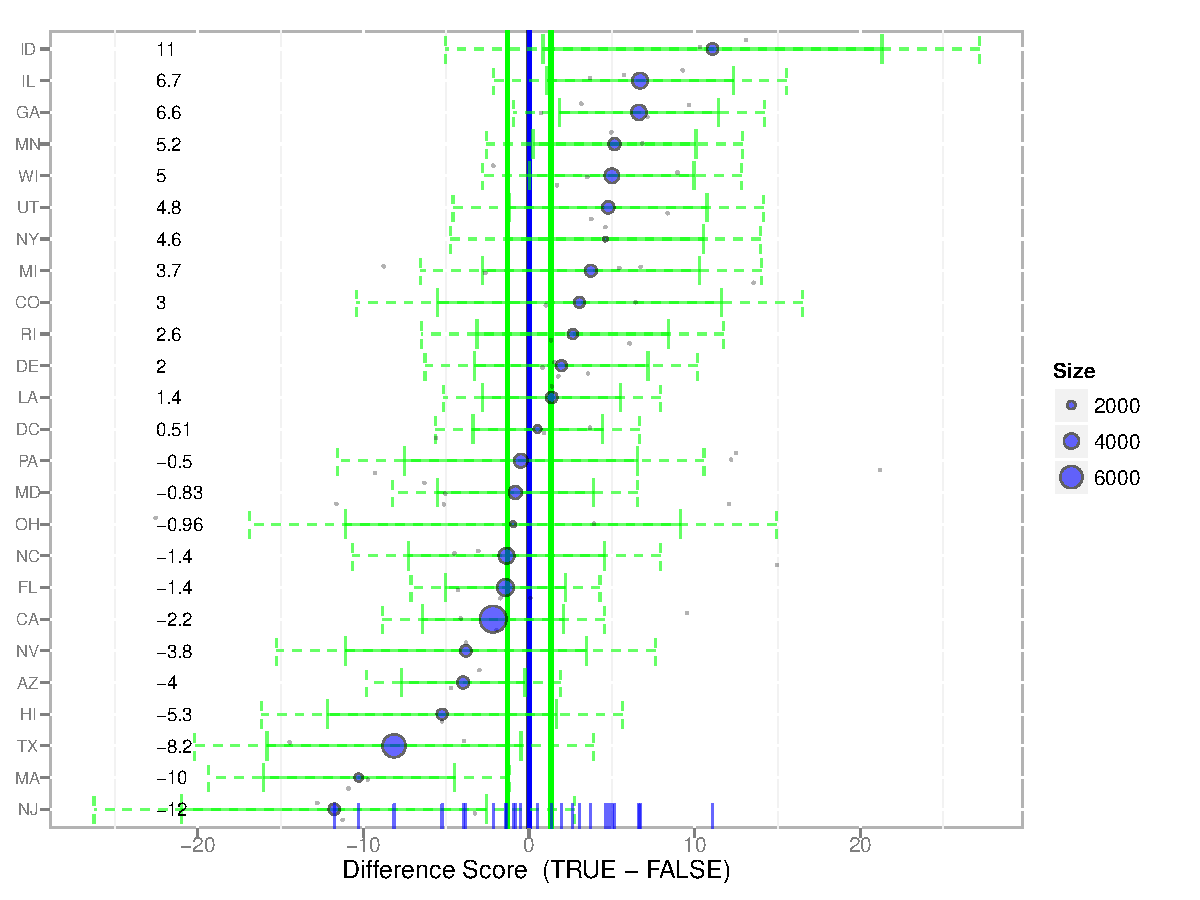
\includegraphics[width=\textwidth]{../Figures2009/g4math-mlpsa-ctree-diff.pdf}
\caption{Multilevel PSA difference plot classification trees: Grade 4 math}
\label{fig:g4math-mlpsa-ctree-diff}
\end{center}
\end{figure}


\clearpage
\subsection{Summary and Overall Results}

Up to this point in the chapter, I have outlined the nine propensity score methods used for estimating treatment effects with grade four math. The corresponding tables and figures have been referenced in the appendices. In this section, I will provide two figures and one table that summarize the 36 propensity score models estimated.

Figure \ref{fig:overallcirc} is a scatter plot of the overall national estimated treatment effects for all 36 PSA methods. The differences across subjects and grades are a result of different scales used for the assessment and therefore comparisons across subject and grade levels is not appropriate. The diameters of the circles in this figure are equal to the confidence interval so that circles that overlap the unit line indicate a non-significant difference. The horizontal and vertical lines (with numeric labels) represent the overall NAEP score for traditional public school students and charter school students. This figure shows that, in general, the scores for charter school students are higher when adjusted, whereas the traditional public school scores are the same or lower. Regardless, in most cases the differences do not deviate substantially from the unit line indicating either no, or a small, difference in scores.

\begin{figure}[t]
\begin{center}
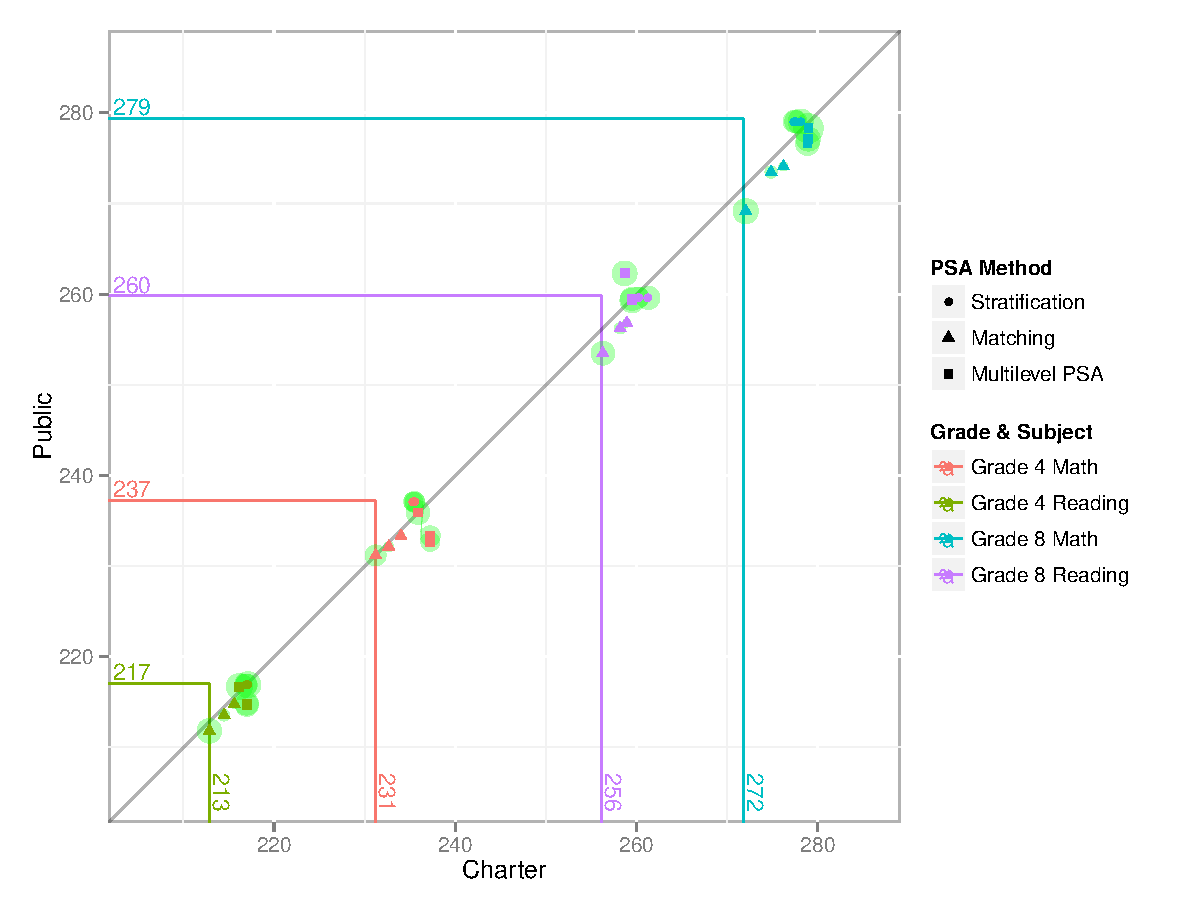
\includegraphics[width=\textwidth]{../Figures2009/OverallScatter.pdf}
\caption{PSA circle plot of adjusted means}
\label{fig:overallcirc}
\end{center}
\end{figure}

Figure \ref{fig:overalldiff} provides the overall national effect sizes for each PSA method within each grade and subject. Table \ref{tab:overall} provides numeric results for this figure. Figure \ref{fig:overalldiff} reveals a number of important results. First, with regard to the effects of charter schools, there is some variety in effects across the different grades and subjects. In general, it appears charter schools either perform worse than or equal to traditional public schools in grade four. Nearly half of the grade eight models in both math and reading suggest small positive effects. However, even when there are statistically significant positive effects, the maximum effect size is relatively small (0.11). 


Figure \ref{fig:overalldiff} also reveals some trends in the behavior of the different propensity score methods. There appears to be fairly good consistency in the estimated effects within the stratification and matching methods, although in general, the matching methods provide larger effect size estimates. However, the matching methods, even with one-to-ten, use fewer than 40\% of the available traditional public school students, whereas the stratification methods use all traditional public school students. There is some variation in the estimated effect sizes for the multilevel models with the classification trees providing larger estimates. As noted above, this may be due, in part, to insufficient balance being achieved. This is likely a limitation of the logistic regression to provide stable estimates given one, the larger charter-to-public school student ratio and two, the smaller samples within each state. The following chapter will provide a discussion of the implications of these results.

\begin{figure}[t]
\begin{center}
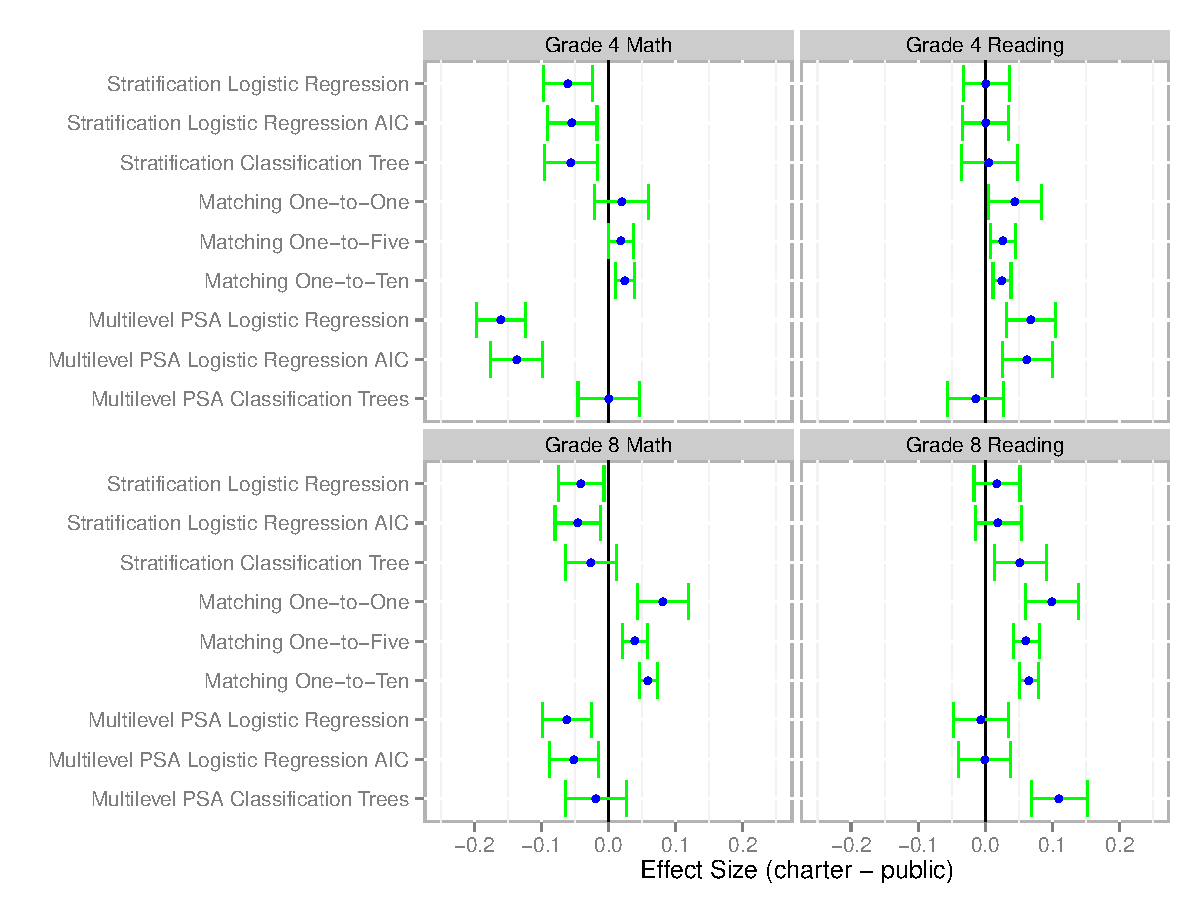
\includegraphics[width=\textwidth]{../Figures2009/Overall.pdf}
\caption{Overall differences in effect size}
\label{fig:overalldiff}
\end{center}
\end{figure}

% latex table generated in R 3.0.1 by xtable 1.7-1 package
% Thu Jun 20 12:52:33 2013
\begin{table}[ht]
\centering
\caption{Summary of overall propensity score results} 
\begin{tabular}{lrrrrr}
  \hline Method & Charter & Public & ATE & \multicolumn{2}{c}{95\% CI} \\   \hline & \multicolumn{5}{c}{Grade 4 Math} \\ \cline{2-6} Stratification Logistic Regression & 235.37 & 237.09 & -0.06 & -2.77 & -0.68 \\ 
  Stratification Logistic Regression AIC & 235.55 & 237.09 & -0.05 & -2.59 & -0.49 \\ 
  Stratification Classification Tree & 235.48 & 237.09 & -0.06 & -2.74 & -0.47 \\ 
  Matching One-to-One & 231.22 & 231.18 & 0.00 & -1.12 & 1.20 \\ 
  Matching One-to-Five & 232.67 & 232.14 & 0.02 & -0.01 & 1.07 \\ 
  Matching One-to-Ten & 234.02 & 233.33 & 0.02 & 0.29 & 1.09 \\ 
  Multilevel PSA Logistic Regression & 237.24 & 232.67 & -0.16 & -3.53 & -5.60 \\ 
  Multilevel PSA Logistic Regression AIC & 237.24 & 233.33 & -0.14 & -2.80 & -5.01 \\ 
  Multilevel PSA Classification Trees & 235.90 & 235.91 & 0.00 & 1.32 & -1.30 \\ 
    \hline & \multicolumn{5}{c}{Grade 4 Reading} \\ \cline{2-6} Stratification Logistic Regression & 216.96 & 216.92 & 0.00 & -1.13 & 1.23 \\ 
  Stratification Logistic Regression AIC & 216.92 & 216.92 & 0.00 & -1.17 & 1.17 \\ 
  Stratification Classification Tree & 217.12 & 216.92 & 0.01 & -1.23 & 1.63 \\ 
  Matching One-to-One & 212.88 & 211.82 & 0.03 & -0.30 & 2.41 \\ 
  Matching One-to-Five & 214.51 & 213.54 & 0.03 & 0.33 & 1.60 \\ 
  Matching One-to-Ten & 215.63 & 214.75 & 0.03 & 0.42 & 1.35 \\ 
  Multilevel PSA Logistic Regression & 217.01 & 214.69 & -0.07 & -1.07 & -3.58 \\ 
  Multilevel PSA Logistic Regression AIC & 216.99 & 214.85 & -0.06 & -0.86 & -3.42 \\ 
  Multilevel PSA Classification Trees & 216.19 & 216.71 & 0.01 & 1.95 & -0.93 \\ 
    \hline & \multicolumn{5}{c}{Grade 8 Math} \\ \cline{2-6} Stratification Logistic Regression & 277.58 & 279.05 & -0.04 & -2.69 & -0.25 \\ 
  Stratification Logistic Regression AIC & 277.41 & 279.06 & -0.05 & -2.86 & -0.43 \\ 
  Stratification Classification Tree & 278.11 & 279.04 & -0.03 & -2.31 & 0.44 \\ 
  Matching One-to-One & 272.05 & 269.16 & 0.08 & 1.51 & 4.28 \\ 
  Matching One-to-Five & 274.85 & 273.46 & 0.04 & 0.72 & 2.06 \\ 
  Matching One-to-Ten & 276.21 & 274.08 & 0.06 & 1.63 & 2.62 \\ 
  Multilevel PSA Logistic Regression & 278.86 & 276.63 & -0.06 & -0.92 & -3.54 \\ 
  Multilevel PSA Logistic Regression AIC & 278.95 & 277.11 & -0.05 & -0.52 & -3.16 \\ 
  Multilevel PSA Classification Trees & 278.98 & 278.30 & -0.02 & 0.94 & -2.30 \\ 
    \hline & \multicolumn{5}{c}{Grade 8 Reading} \\ \cline{2-6} Stratification Logistic Regression & 260.20 & 259.63 & 0.02 & -0.55 & 1.69 \\ 
  Stratification Logistic Regression AIC & 260.25 & 259.63 & 0.02 & -0.49 & 1.74 \\ 
  Stratification Classification Tree & 261.30 & 259.60 & 0.05 & 0.43 & 2.97 \\ 
  Matching One-to-One & 256.29 & 253.48 & 0.09 & 1.51 & 4.12 \\ 
  Matching One-to-Five & 258.19 & 256.24 & 0.06 & 1.33 & 2.58 \\ 
  Matching One-to-Ten & 258.93 & 256.82 & 0.06 & 1.65 & 2.57 \\ 
  Multilevel PSA Logistic Regression & 259.51 & 259.30 & -0.01 & 1.13 & -1.55 \\ 
  Multilevel PSA Logistic Regression AIC & 259.52 & 259.49 & -0.00 & 1.24 & -1.31 \\ 
  Multilevel PSA Classification Trees & 258.70 & 262.29 & 0.11 & 4.96 & 2.23 \\ 
   \hline
\end{tabular}
\label{tab:overall}
\end{table}


\subsection{Differences Between States}

The National Alliance for Public Charter Schools (NAPCS) publishes annually rankings of state charter school laws \cite{NAPCS2012}. They argue that some of the performance of charter schools in some states may be hindered by state law. Figure \ref{fig:staterankings} is a slepegraph \cite{Tufte2001} that compares the rankings given to each state by NAPCS with that state's ranking using stratification with classification trees\footnote{A slopegraph for only the stratification with classification trees is provided since 1) it resulted in better balance as compared to the other methods, and 2) the results are consistent regardless of method used.}. Although top rated states by NAPCS had larger differences in NAEP scores, there is considerable crossing of lines between the two rankings. This visual cue indicates that the rankings are not very correlated. It should also be noted that not all states that have charter laws had sufficient sample size in NAEP to be included.

\begin{figure}[t]
\begin{center}
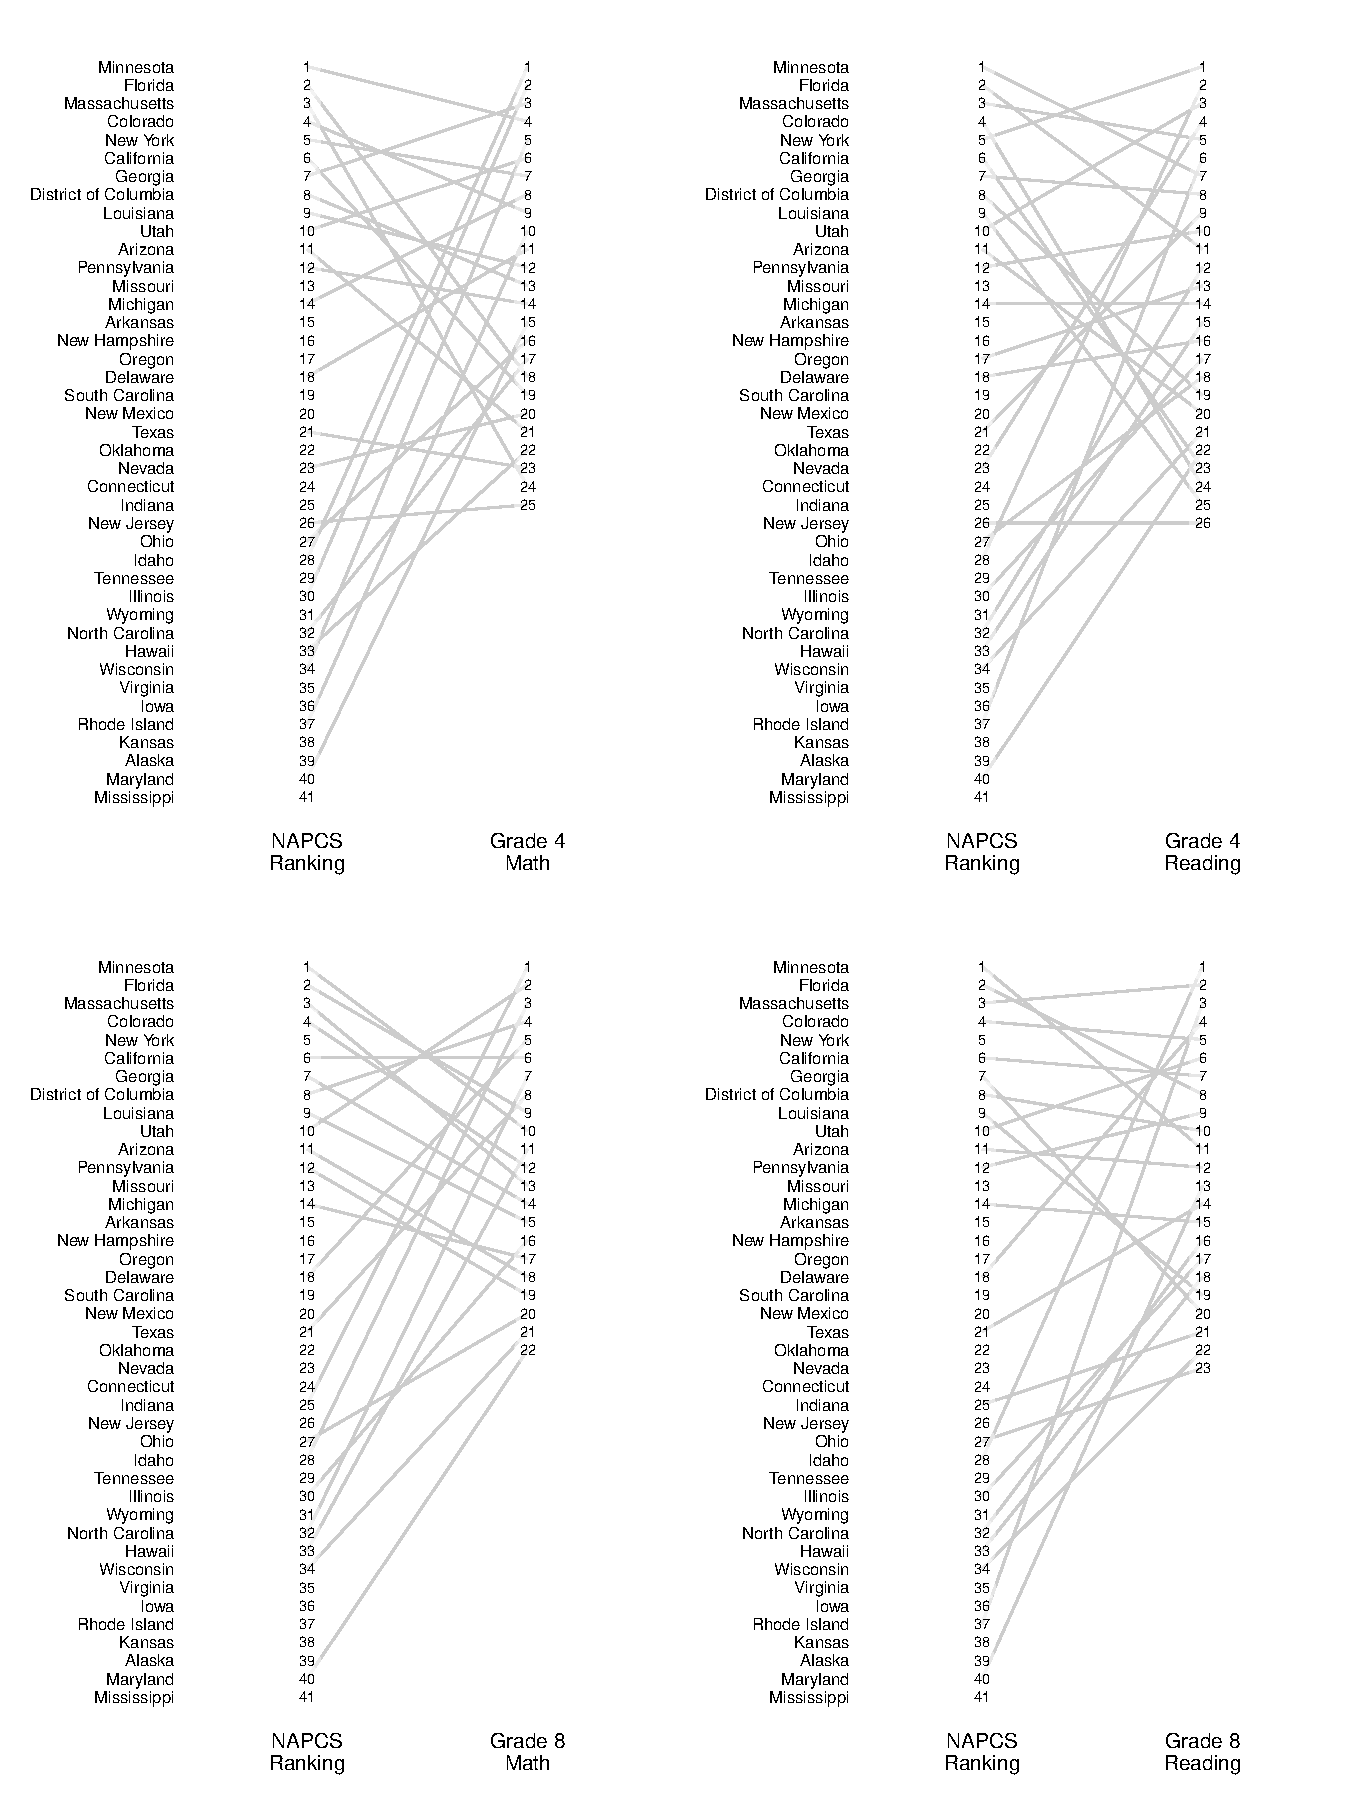
\includegraphics[width=\textwidth]{../Figures2009/StateRankings.pdf}
\caption{Comparison of 2012 National Alliance for Public Charter Schools (NAPCS) state charter school law rankings and NAEP charter school rankings}
\label{fig:staterankings}
\end{center}
\end{figure}


%==================== CHAPTER 5 ====================================================================
\cleardoublepage
\section{Chapter 5: Discussion}

This study aims to make two major contributions: first, address the question of the effectiveness of charter schools from a state and national perspective, and second, develop a new method of propensity score analysis for multilevel data to facilitate answering the research questions. This chapter will interpret the results as well as point out some limitations of this study.

\subsection{Discussion of Research Questions}

This study set out to address three research questions regarding the differences between charter and traditional public schools. The first two questions regarding differences between student performance will be addressed together in the following section. The relationship between state differences and charter school laws will be discussed separately.

\subsubsection{Differences between charter and traditional public schools}

The purpose of this study was to answer: Given appropriate adjustments based on available student data, is there a discernible difference between charter and traditional public schools with regard to math and reading scores on the NAEP evaluated at grades 4 and 8  And if so, what is the nature and magnitude of this difference for the two outcomes, in reading and mathematics? Of the 36 different propensity score models estimated, 11 resulted in a positive effect for charter schools, another 11 resulted in a positive effect for traditional public schools, and the remaining 14 resulted in no difference (see Figure \ref{fig:overalldiff} and Table \ref{tab:overall}). Across all models, effect sizes ranged from -0.16 to 0.11, all considered very small by virtually all statistical standards \cite<c.f.> {Cohen1988}. In aggregate, and given the available data, there is no discernible difference in the performance of charter and traditional public school students in grade 4 and 8 math and reading in NAEP.

Given the substantial difference in sample \textit{n}'s for charter and public schools (i.e. there are as much as three to four orders of magnitude more public schools students available in the NAEP data sets), it is expected that there would be public school students who would not have a counterpart from the charter school group. However, the relatively high percentage of public schools students who do not have a charter school counterpart (as much as 35\%) suggest that there may be imbalance between the two groups as a whole. That is, although reasonable balance was achieved with regard to the individual strata where comparisons are made, the overall sample imbalance, as evidenced by the unmatched public school students, suggests that public schools serve a more heterogeneous population. The nature of the demographic differences between charter and traditional public school students should be explored in a future study.

%Moreover, the methodological issues described below, in part, be evidence of any underlying fundamental difference in charter school and traditional public school populations. Figure \ref{fig:overalldiff} in chapter four reveals that the methods with higher effect sizes are the matching methods and classification trees. These models, especially the matching methods, often eliminate a large proportion of tradition public school students. Perhaps there may be a small positive effect of charter schools for a very specific type of student, but there also appears to be a large number of students who appear better served, or at least equivalently served, by traditional public schools. This needs to be considered when weighing the cost and extent of charter schools.

\subsubsection{State charter laws and charter school performance}

\citeA{BraunJenkinsGrigg2006} suggested that there are environmental (political and policy) influences on the performance of charter schools. Additionally, The National Alliance for Public Charter Schools \cite<NAPCS;>{NAPCS2012} publishes annually rankings of state charter laws in part, because they believe that poor charter school laws can hinder the performance of students in charter schools. Given that the results of the multilevel PSA provide a natural ranking based upon student differences within each state, this afforded an opportunity to test whether there is a relationship between state laws and student performance in NAEP. However, comparing the rankings from the multilevel PSA along with the NAPCS state charter law rankings suggest that there is no relationship between charter laws and student performance (see Figure \ref{fig:staterankings}).

\subsection{Discussion of Research Methods}

In order to address the research questions discussed above, a new class of propensity score method was developed for multilevel, or clustered data. The results of this study indicate that this method provides estimates that are consistent with more traditional approaches to PSA. However, this method provides important insight into the relationship of clusters not available in other methods. This section will address the methodological implications of this study.

\subsubsection{Multilevel Propensity Score Analysis}

The development of the \texttt{multilevelPSA} R package for estimating and visualizing propensity score models of multilevel data provides important insight into the implications of what traditionally would have been one of many covariates. The results suggest that this method performs and provides effect size estimates consistent with other propensity score methods. However, a key advantage to using this new method includes an explicit adjustment of the multilevel nature of some data as well as being able to understand the implication of clustering when comparing the outcome of interest. As researchers work with larger and larger datasets, the advancements in data visualization should be taken advantage of. The data visualizations developed for this dissertation provide important insight into data analysis at all stages.

Propensity score methods have shown to be effective for estimating treatment effects with relatively small samples. However, as observed in chapter four, estimating multilevel PSA models requires larger samples given the need to stratify within clusters. Although NCES began oversampling charter schools in 2005, the fact that the ratio of charter to traditional public schools/students is so large results in model specification problems, especially with logistic regression. This has been alleviated to some extent by removing traditional public school students who attend a school farther than five miles from a charter school. 

More specifically with regard to propensity score ranges, the range tends to shrink as the ratio of treatment-to-control increases. Figure \ref{fig:psranges} depicts the range and distribution of propensity scores (using logistic regression) with varying treatment-to-control ratios. The data used to create this figure is simulated and available in Appendix K. The \texttt{psrange} and \texttt{plot.psrange} functions are included in the \texttt{multilevelPSA} R package. Propensity scores are estimated with a single covariate where the mean for the treatment and control are 0.6 and 0.4, respectively. The standard deviation for both is 0.4. There are 100 treatment units and 1,000 control units simulated. The goal in choosing these means and standard deviations is to have some separation between treatment and control. Each row in the figure represents the percentage of control units sampled before estimating the propensity scores starting with 100\% (i.e. all 1,000 control units) to 10\% (100 of the control units). As the figure shows, as the ratio decreases to where there are equal treatment and control units, the range of the propensity scores becomes more normal. To calculate the ranges, each sampling step is bootstrapped so the green bar and black points represent each of the 20 bootstrap samples taken. The bars then represent the mean of the minimum and mean of the maximum for each step.

\begin{figure}[t]
\begin{center}
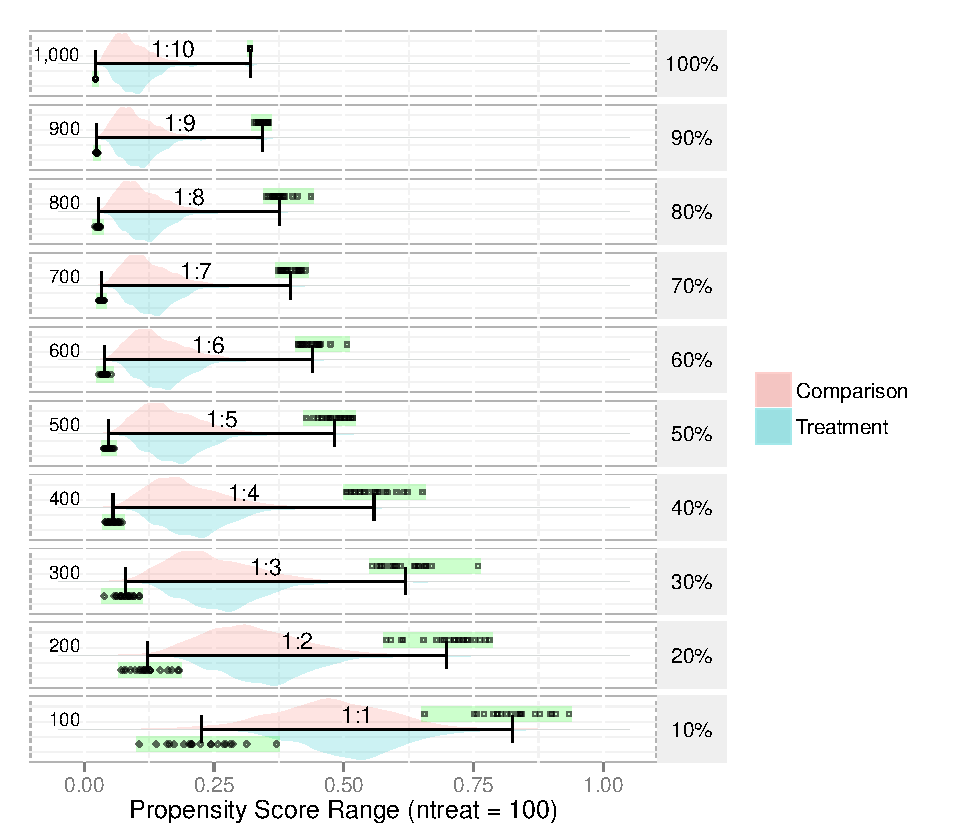
\includegraphics[width=\textwidth]{../Figures2009/PSRanges.pdf}
\caption{Propensity score ranges for varying treatment-to-control ratios}
\label{fig:psranges}
\end{center}
\end{figure}

\subsubsection{The Display of Multilevel Results}

In the development of the \texttt{multilevelPSA}, as well as all the analysis in the dissertation, two overarching principal decisions were made with regard to how results are displayed, specifically the lack of \textit{p}-values and an emphasis on visualizations over tabular output. Both of these issues have received substantial attention and debate over the last several decades. And although there is no clear consensus on ``best-practices," I contend that given the nature of propensity score analysis and observational studies, simple null hypotheses reported as either statistically significant or not in tables with \texttt{p}-values does a disservice to the results. The use of graphics with confidence intervals provide context as well as magnitudes of differences.

% p-values

The practice of significance testing\footnote{Here, I use the phrases significance testing, null hypothesis testing, and \textit{p}-values to represent the same statistical practice and are generally interchangeable.} dates to the early work of \citeA{Fisher1925}. \citeA{Gigerenzer2004} describes the current practice in peer-reviewed research journals as ``the null ritual" that involves three steps:

\begin{enumerate}
    \item Define a null hypothesis where the researcher is testing that there is no mean difference. Do not specify any predictions or alternative hypotheses.
    \item Use a \textit{p}-value of .05 for rejecting the null hypothesis and report your \textit{p}-value using a range (i.e. \textit{p} \textless .05, \textit{p} \textless .01, or \textit{p} \textless .001).
    \item Always perform this procedure.
\end{enumerate}

\noindent In 1996 the American Psychological Association (APA) brought the debate regarding the use of significance testing to the forefront by entertaining a ban in the journals it publishes \cite{Shrout1997,Hunter1997,Harris1997,Abelson1997,Scarr1997,Estes1997}. Although a ban was not instituted, APA now recommends the reporting of exact \textit{p}-values, confidence intervals, and effect sizes. 

What is the issue with \textit{p}-values First, the practice of significance testing as represented in the social sciences for nearly the last century reduce research questions to a dichotomous outcome. Rarely can a study be reduced to a simple yes/no answer, especially in the social sciences. Moreover, the use of \textit{p} \textless .05 is entirely arbitrary and the difference between significant and non-significant results is itself not significant \cite{GelmanStern2006}. However, perhaps more damning is the likelihood of committing Type II errors \cite{Bakan1966,Carver1978,Cohen1994,HenkelMorrison1970,Rozeboom1960,Schmidt1996}. In a study by \citeA{SedlmeierGigerener1989} that examined all published articles in 1984 in the \textit{Journal of Abnormal Psychology} found that the error rate was 60\%. That is to say that researchers would have done better to flip a coin!

Lastly, given the relationship between \textit{p}-values and sample size, it would be expected that with \textit{n} \textgreater 100,000, as in this study, most differences would be statistically significant. Even in one-to-one matched analysis where $n \approx 3,000$, we would expect \textit{p} \textless 0.05 for even small differences. The formula for calculating \textit{t} for a dependent sample paired \textit{t}-test is:

$$ t = \frac{{\bar{X}_D} - \mu_0}{S_D / \sqrt{n}} $$

\noindent Where $X_D$ is the mean difference, $\mu_0$ is non-zero for testing differences other than zero, $S_D$ is the standard deviation of the differences, and $n$ is the sample size. Using the approximate sample standard deviation of 40 from grade 8 reading results, a mean difference 2 (representing a small effect size of 0.06 by most standards), and $n = 3000$, we get $t = 2.738$ and $p = 0.003$. For the one-to-one paired analysis with a very small effect size the power estimate \cite{Cohen1988} is 0.64. However, the one-to-two matched analysis increases the power to a very acceptable 0.90. The results of this exercise is to demonstrate that relying on \textit{p}-values to make decisions is a \textit{fool's errand}. Instead, we should take Scarr's suggestion that ``better uses of statstics would focus on the magnitude of effects and error estimates" \cite{Scarr1997}.

The use of graphics have made substantial advancements in the twentieth century with seminal works by Tukey \cite{Cleveland1988}, \citeA{Tufte2001}, \citeA{Cleveland1993,Cleveland1994}, and \citeA{Chambers1983}. The implementations utilized in this dissertation are based upon \citeauthor{Wilkinson2005}'s \citeyear{Wilkinson2005} \textit{grammar of graphics} as implemented in R using the \texttt{ggplot2} package \cite{Wickham2009}. Wherever possible, confidence intervals are used to show the magnitude of the differences \cite<c.f.>{Cumming2012,Estes1997a}. Although the use of graphics are frequently taught in statistics courses, they are often omitted from journal publications \cite{GelmanPasaricaDodhia2002} and relegated to diagnostic purposes \cite{Gelman2011}. The graphics presented here provide important insight into the nature and magnitude of the differences between charter and traditional public schools. The multilevel assessment plots (see Figure \ref{fig:g4math:circpsa} and Appendix H) show the distribution scores (charter, traditional public, and differences) across multiple dimensions simultaneously. Perhaps we would see from a table that the differences are small within states with few exceptions. But what would be lost is that the range of scores across states for charter and traditional public school students separately is relatively wide. Similarly, for the multilevel PSA difference plots (see Figure \ref{fig:g4math-mlpsa-ctree-diff} and Appendix H) the graphic provides immediate evidence of the nature of the differences. Also, by providing confidence intervals, we can express results vis-à-vis the graphic similar to the traditional \textit{p}-value in a summary table.

\subsection{Limitations}

This study, and many like it, only examined a small subset of a students educational experiences. That is, NAEP, as well as CREDO \cite{credo,credo2013}, only examine student performance in math and reading. This leaves out all other, and arguably equally important, subjects. These studies are not alone in overemphasizing these subjects. The Common Core State Standards which is being implemented in the majority of states and is a cornerstone of the \textit{Race to the Top} initiative, only defines standards and curriculum for mathematics and English Language Arts. The emphasis on only these two subjects has resulted in many schools reducing or eliminating the arts and other subjects to spend more school time preparing students in these subjects \cite<c.f.>{Ravitch2013}.

Although no relationship between state charter law rankings and student differences was found, this only addresses one part of the charter school governing process. That is, state laws are not the only thing dictating how charter schools operate. There are many charter granting bodies and these may differ from region-to-region, city-to-city, and even from school-to-school. 

Lastly, this study considered charter schools as an entire, single class of schools. I believe it is important to explore the effectiveness of charter schools as compared to traditional publics schools, especially given that some cities (e.g. New Orleans and Philadelphia) have the majority of their students attending charter schools as well as the Department of Education emphasizing charter school expansion as part of the \textit{Race to the Top} initiative. However, this study, and other national studies like it \cite<e.g.>{BraunJenkinsGrigg2006,credo}, does not explicitly account for the large variability in quality of individual charter schools. Although, this study does provide some evidence that there is indeed wide variability in those differences (mostly as a feature of the visualizations utilized). Consider the multilevel PSA difference plots (e.g. Figure \ref{fig:g4math-mlpsa-ctree-diff}) where the grey points represent the difference for each strata. The spread of these points is quite large and indeed there are some strata with much larger gains than the overall aggregate. This suggests that, for some very specific types of students, charter schools provide much larger gains over their traditional school student counterparts. Indeed, this should be expected given \citeauthor{Budde1988}'s \citeyear{Budde1988} original vision and model for charter schools. That is, charter schools provide an opportunity for teachers, administrators, parents, and communities to experiment with alternative school models. Future studies should consider the varying types of charter schools (e.g. for-profit, non-profit, KIPP, online) along with traditional public schools. And moreover, we need to explore those schools and students so that the features of those schools are incorporated back into all other schools.

\clearpage

\subsection{Conclusion}

In summary, the results of this study are consistent with the wide body of research on charter schools. Namely, some charter schools are better than their traditional public school counterpart, while others perform worse. However, in aggregate, the average difference is nonexistent, or very small. Ray Budde originally envisioned charter schools as a way for teachers, administrators, parents, and communities to experiment with the goal of finding better ways to teach students. But with \textit{No Child Left Behind} and \textit{Race to the Top}, among other initiatives from private for-profit and not-for-profit organizations, charter schools are often offered as a wholesale replacement for traditional public schools. However, these results along with the other national studies examining the differences between charter and traditional public schools suggest that charter schools do not provide, in aggregate, substantial benefit over their traditional public school counterparts.



%==================== REFERENCES ====================================================================
\cleardoublepage
\bibliographystyle{apacite}
\bibliography{Bibliography}

\newpage

%==================== Appendices ====================================================================
\cleardoublepage
\addcontentsline{toc}{section}{Appendices}
\appendix

% For large tables, use this just before the \begin{tabular}
%\resizebox{\linewidth}{!}{%

%==================== Appendix A ====================================================================
\renewcommand{\thefootnote}{\fnsymbol{footnote}}% Change the footnote style to lowercase letters
\addcontentsline{toc}{subsection}{Appendix A: Charter School \& Student Enrollment by State}
\section*{Appendix A\\Charter Schools \& Student Enrollment by State}
\label{appendixA}
\begin{center} \begin{singlespace}
\begin{longtable}{lrrrrrrr}
\caption[Charter schools \& student enrollment by state]{Charter schools \& student enrollment by state} \\
\thickline
      & Law     & \multicolumn{3}{c}{Totals for Charter Schools\tabfnm{b}}              & & \multicolumn{2}{c}{NAEP Students}\\
\cline{3-5} \cline{7-8}
State & Enacted & Operating & Closed & Students & & Charters & Publics\\
\hline
\endfirsthead
\multicolumn{8}{l}{Charter Schools \& Student Enrollment by State (cont.)}\\
\hline
      & Law     & \multicolumn{3}{c}{Totals for Charter Schools\tabfnm{b}}              & & \multicolumn{2}{c}{NAEP Students}\\
\cline{3-5} \cline{7-8}
State & Enacted & Operating & Closed & Students & & Charters & Publics\\
\hline
\endhead
\hline 
\endfoot
\thickline
\endlastfoot
Alabama\tabfnm{a}       &      & 0   & 0   & 0       & &   0 & 2759\\
Alaska                  & 1995 & 26  & 5   & 5,198   & &  69 & 2517\\
Arizona                 & 1994 & 510 & 96  & 119,903 & &  99 & 2674\\
Arkansas                & 1995 & 25  & 6   & 6,750   & &  30 & 2407\\
California              & 1992 & 802 & 103 & 316,468 & & 417 & 7803\\
Colorado                & 1993 & 151 & 10  & 54,497  & & 108 & 2598\\
Connecticut             & 1996 & 21  & 5   & 3,932   & &   0 & 2531\\
Delaware                & 1995 & 21  & 2   & 8,740   & & 180 & 2641\\
Washington DC           & 1996 & 93  & 16  & 25,385  & & 652 & 1336\\
Florida                 & 1996 & 382 & 82  & 108,382 & & 175 & 3876\\
Georgia                 & 1993 & 83  & 5   & 40,807  & &  64 & 3465\\
Hawaii                  & 1994 & 32  & 0   & 7,317   & & 132 & 2605\\
Idaho                   & 1998 & 32  & 1   & 10,492  & &  59 & 2784\\
Illinois                & 1996 & 74  & 8   & 27,683  & &  33 & 4015\\
Indiana                 & 2001 & 50  & 2   & 12,631  & &  11 & 2720\\
Iowa                    & 2002 & 10  & 0   & 1,462   & &   0 & 2839\\
Kansas                  & 1994 & 40  & 10  & 3,361   & &  17 & 2726\\
Kentucky\tabfnm{a}      &      & 0   & 0   & 0       & &   0 & 2696\\
Louisiana               & 1995 & 66  & 10  & 23,634  & &  97 & 2264\\
Maine\tabfnm{a}         &      & 0   & 0   & 0       & &   0 & 2658\\
Maryland                & 2003 & 34  & 2   & 7,301   & &   6 & 2825\\
Massachusetts           & 1993 & 64  & 6   & 23,905  & &  56 & 3667\\
Michigan                & 1993 & 250 & 27  & 94,092  & & 134 & 2480\\
Minnesota               & 1991 & 159 & 29  & 28,371  & &  16 & 2875\\
Mississippi             & 1997 & 1   & 0   & 367     & &   0 & 2613\\
Missouri                & 1998 & 39  & 5   & 13,125  & &  38 & 2771\\
Montana\tabfnm{a}       &      & 0   & 0   & 0       & &   0 & 2581\\
Nebraska\tabfnm{a}      &      & 0   & 0   & 0       & &   0 & 2688\\
Nevada                  & 1997 & 26  & 7   & 7,295   & &   0 & 2662\\
New Hampshire           & 1995 & 11  & 2   & 1,212   & &   0 & 2803\\
New Jersey              & 1996 & 64  & 19  & 17,986  & &   0 & 2813\\
New Mexico              & 1993 & 70  & 3   & 11,426  & &  54 & 2722\\
New York                & 1998 & 118 & 10  & 32,602  & &  16 & 3745\\
North Carolina          & 1996 & 103 & 32  & 30,445  & &  72 & 4090\\
North Dakota\tabfnm{a}  &      & 0   & 0   & 0       & &   0 & 2307\\
Ohio                    & 1997 & 293 & 48  & 94,171  & &  45 & 3746\\
Oklahoma                & 1999 & 14  & 1   & 4,770   & &   0 & 2612\\
Oregon                  & 1999 & 93  & 8   & 13,612  & &  41 & 2626\\
Pennsylvania            & 1997 & 133 & 12  & 61,823  & &  64 & 2709\\
Rhode Island            & 1995 & 11  & 0   & 2,894   & &  30 & 2621\\
South Carolina          & 1996 & 36  & 10  & 8,705   & &  16 & 2697\\
South Dakota\tabfnm{a}  &      & 0   & 0   & 0       & &   0 & 2889\\
Tennessee               & 2002 & 14  & 1   & 2,585   & &  54 & 2815\\
Texas                   & 1995 & 331 & 33  & 108,541 & & 199 & 7070\\
Utah                    & 1998 & 68  & 1   & 23,233  & &  38 & 2722\\
Vermont\tabfnm{a}       &      & 0   & 0   & 0       & &   0 & 2003\\
Virginia                & 1998 & 4   & 3   & 275     & &   0 & 2848\\
Washington\tabfnm{a}    &      & 0   & 0   & 0       & &   0 & 2968\\
West Virginia\tabfnm{a} &      & 0   & 0   & 0       & &   0 & 2831\\
Wisconsin               & 1993 & 221 & 37  & 41,799  & & 114 & 2592\\
Wyoming                 & 1995 & 3   & 0   & 244     & &   0 & 1897\\
\hline
Total                   &      & 4,578 & 657 & 1,407,421 & & 3,164 & 156,963 \\
\end{longtable}
\tabfnt{a}{State currently does not have a charter school law.}
\tabfnt{b}{Source: \citeA{cernumbers}}
\end{singlespace} \end{center}
\renewcommand{\thefootnote}{\arabic{footnote}}% Reset the footnotes back to numbers


%==================== Appendix B ====================================================================
\newpage
\addcontentsline{toc}{subsection}{Appendix B: Descriptive Statistics}
\section*{Appendix B\\Descriptive Statistics}
\label{appendixB}

\begin{singlespace}

\input{../Tables2009/g4Math-desc.tex}
% latex table generated in R 3.0.0 by xtable 1.7-1 package
% Fri May 31 15:00:30 2013
\begin{sidewaystable}[ht]
\centering
\caption{Grade 4 Math Unadjusted NAEP Score} 
\label{tab:g4math-unadjscore}
\begin{tabular}{lrrrrrr@{\extracolsep{10pt}}rrrrrr}
  \hline & \multicolumn{6}{c}{Charter Schools} & \multicolumn{6}{c}{Public Schools} \\ \cline{2-7} \cline{8-13} & n & mean & sd & median & min & max & n & mean & sd & median & min & max \\ 
  \hline
Overall & 3625 & 231.93 & 28.19 & 232.18 & 136.95 & 310.45 & 159338 & 238.34 & 27.71 & 239.71 & 117.69 & 334.07 \\ 
  Alaska & 102 & 247.41 & 24.64 & 248.79 & 183.80 & 296.82 & 2496 & 238.50 & 28.87 & 240.91 & 133.70 & 314.90 \\ 
  Arkansas & 226 & 229.38 & 29.27 & 230.22 & 145.74 & 294.08 & 2836 & 228.66 & 29.47 & 229.71 & 142.09 & 324.86 \\ 
  Canal zone & 170 & 223.41 & 26.86 & 221.21 & 152.40 & 290.14 & 7241 & 227.05 & 30.42 & 227.52 & 127.08 & 330.95 \\ 
  Connecticut & 132 & 250.45 & 28.67 & 256.63 & 148.19 & 308.90 & 2550 & 242.34 & 28.39 & 244.89 & 130.83 & 317.99 \\ 
  D.C. & 512 & 217.48 & 26.97 & 215.26 & 146.95 & 306.62 & 1282 & 219.99 & 32.15 & 219.20 & 133.26 & 317.28 \\ 
  Florida & 195 & 240.20 & 26.34 & 238.76 & 168.45 & 294.30 & 2586 & 239.42 & 24.64 & 239.68 & 159.44 & 316.57 \\ 
  Idaho & 166 & 241.09 & 24.28 & 244.36 & 175.09 & 293.17 & 4531 & 239.76 & 24.97 & 240.17 & 147.51 & 324.61 \\ 
  Illinois & 164 & 241.86 & 25.56 & 244.89 & 183.18 & 310.45 & 3865 & 232.69 & 28.18 & 232.54 & 140.58 & 316.17 \\ 
  Iowa &  57 & 230.95 & 26.26 & 234.88 & 146.85 & 273.46 & 2695 & 236.28 & 31.24 & 239.72 & 127.32 & 314.05 \\ 
  Kansas &  60 & 255.08 & 20.79 & 255.56 & 183.42 & 300.83 & 3024 & 240.97 & 24.84 & 242.25 & 139.84 & 314.77 \\ 
  Kentucky &  78 & 229.74 & 27.71 & 231.49 & 147.64 & 295.55 & 4059 & 232.94 & 29.83 & 233.75 & 117.69 & 318.75 \\ 
  Michigan &  65 & 230.80 & 16.68 & 230.98 & 197.30 & 279.19 & 2830 & 229.16 & 24.90 & 229.32 & 144.26 & 308.71 \\ 
  Mississippi & 141 & 219.12 & 26.52 & 217.25 & 164.93 & 293.18 & 3249 & 239.22 & 27.40 & 238.06 & 148.45 & 318.09 \\ 
  Missouri &  52 & 229.29 & 22.62 & 226.30 & 179.65 & 284.75 & 3615 & 248.36 & 25.63 & 249.08 & 145.76 & 317.96 \\ 
  Montana & 215 & 218.06 & 29.43 & 216.04 & 136.95 & 288.98 & 3204 & 229.38 & 31.66 & 231.15 & 128.36 & 318.70 \\ 
  Nebraska & 109 & 247.68 & 26.51 & 248.08 & 188.30 & 302.32 & 3204 & 248.59 & 27.03 & 251.09 & 150.58 & 323.00 \\ 
  New York &  72 & 231.01 & 31.20 & 229.16 & 162.07 & 303.29 & 2977 & 234.90 & 25.81 & 236.10 & 137.78 & 303.75 \\ 
  North Dakota &  74 & 224.15 & 23.57 & 223.48 & 179.04 & 284.71 & 2780 & 247.30 & 26.13 & 249.06 & 155.28 & 325.63 \\ 
  Oklahoma &  60 & 229.73 & 21.88 & 230.70 & 189.84 & 269.90 & 3997 & 239.50 & 26.83 & 240.45 & 145.65 & 315.10 \\ 
  Oregon &  96 & 249.72 & 19.40 & 250.68 & 206.39 & 290.68 & 4320 & 243.07 & 26.92 & 243.12 & 130.47 & 323.33 \\ 
  Rhode Island & 124 & 218.15 & 22.02 & 217.22 & 159.99 & 269.17 & 3324 & 237.62 & 29.58 & 239.43 & 126.61 & 319.60 \\ 
  Utah &  79 & 230.94 & 23.07 & 227.57 & 185.38 & 297.38 & 2404 & 239.08 & 28.41 & 241.89 & 136.10 & 307.88 \\ 
  Washington &  91 & 231.23 & 20.75 & 229.44 & 166.83 & 278.23 & 6193 & 238.97 & 24.48 & 239.19 & 139.25 & 317.06 \\ 
  West Virginia & 197 & 247.20 & 25.79 & 250.06 & 164.01 & 305.53 & 3145 & 239.22 & 28.47 & 241.50 & 130.38 & 319.46 \\ 
  DoDEA/DDESS & 136 & 229.43 & 26.14 & 226.78 & 178.41 & 289.56 & 3694 & 237.95 & 29.14 & 239.24 & 134.42 & 320.51 \\ 
   \hline
\end{tabular}
\end{sidewaystable}
 \clearpage

% latex table generated in R 3.0.1 by xtable 1.7-1 package
% Wed Jun 19 20:22:03 2013
\begin{longtable}{lrr@{\extracolsep{10pt}}rr}
\caption{Grade 4 Reading Descriptive Statistics} \\ 
   \thickline & \multicolumn{2}{c}{Traditional} & \multicolumn{2}{c}{Charter} \\  \endfirsthead \multicolumn{5}{l}{{...continued from previous page}}\\ \hline & \multicolumn{2}{c}{Charter} & \multicolumn{2}{c}{Traditional}  \\ \hline \endhead \thickline \multicolumn{5}{r}{continued on next page...} \\ \endfoot \multicolumn{5}{c}{} \\ \endlastfoot  \pagebreak[2] \hline \multicolumn{5}{c}{Race/ethnicity from school records (raw data)} \\ \cline{1-5} White & 96992 & 58\% & 1343 & 34\% \\ 
  Black & 29127 & 17\% & 1636 & 42\% \\ 
  Hispanic & 28133 & 17\% & 705 & 18\% \\ 
  Asian Amer/Pacif Is & 8114 & 5\% & 162 & 4\% \\ 
  Amer Ind/Alaska Nat & 3898 & 2\% &  49 & 1\% \\ 
  Other & 2333 & 1\% &  41 & 1\% \\ 
  Unknown &   0 & 0\% &   0 & 0\% \\ 
   \pagebreak[2] \hline \multicolumn{5}{c}{Natl School Lunch Prog eligibility (3 categories)} \\ \cline{1-5} Eligible & 82354 & 49\% & 2223 & 56\% \\ 
  Not eligible & 85304 & 51\% & 1528 & 39\% \\ 
  Info not available & 939 & 1\% & 185 & 5\% \\ 
  Unknown &   0 & 0\% &   0 & 0\% \\ 
   \pagebreak[2] \hline \multicolumn{5}{c}{Student has Individualized Education Plan} \\ \cline{1-5} Yes, IEP & 16579 & 10\% & 307 & 8\% \\ 
  Yes, 504 plan & 1385 & 1\% &  29 & 1\% \\ 
  Yes, 504 in process &   0 & 0\% &   0 & 0\% \\ 
  Not IEP & 150596 & 89\% & 3600 & 91\% \\ 
  Omitted &   0 & 0\% &   0 & 0\% \\ 
  Unknown &  37 & 0\% &   0 & 0\% \\ 
   \pagebreak[2] \hline \multicolumn{5}{c}{Student classified Eng Lang Learner (3 categories)} \\ \cline{1-5} Yes & 12095 & 7\% & 285 & 7\% \\ 
  No & 153110 & 91\% & 3569 & 91\% \\ 
  Formerly ELL & 3357 & 2\% &  82 & 2\% \\ 
  Omitted &   0 & 0\% &   0 & 0\% \\ 
  Unknown &  35 & 0\% &   0 & 0\% \\ 
   \pagebreak[2] \hline \multicolumn{5}{c}{Gender} \\ \cline{1-5} Male & 85214 & 51\% & 1960 & 50\% \\ 
  Female & 83383 & 49\% & 1976 & 50\% \\ 
  Unknown &   0 & 0\% &   0 & 0\% \\ 
   \pagebreak[2] \hline \multicolumn{5}{c}{Student classified as having a disability (504)} \\ \cline{1-5} Student with disabi & 17964 & 11\% & 336 & 9\% \\ 
  Not student with di & 150596 & 89\% & 3600 & 91\% \\ 
  Omitted &  37 & 0\% &   0 & 0\% \\ 
  Unknown &   0 & 0\% &   0 & 0\% \\ 
   \pagebreak[2] \hline \multicolumn{5}{c}{Student classified SD or ELL} \\ \cline{1-5} Student with disabi & 16722 & 10\% & 314 & 8\% \\ 
  English language le & 10853 & 6\% & 263 & 7\% \\ 
  Both SD and ELL & 1242 & 1\% &  22 & 1\% \\ 
  Neither SD nor ELL & 139727 & 83\% & 3337 & 85\% \\ 
  Unknown &  53 & 0\% &   0 & 0\% \\ 
   \pagebreak[2] \hline \multicolumn{5}{c}{Newspaper in home} \\ \cline{1-5} Yes & 47839 & 28\% & 1141 & 29\% \\ 
  No & 59247 & 35\% & 1327 & 34\% \\ 
  I Don't Know & 58294 & 35\% & 1343 & 34\% \\ 
  Omitted & 3205 & 2\% & 125 & 3\% \\ 
  Multiple &  12 & 0\% &   0 & 0\% \\ 
  Unknown &   0 & 0\% &   0 & 0\% \\ 
   \pagebreak[2] \hline \multicolumn{5}{c}{Magazines in home} \\ \cline{1-5} Yes & 95695 & 57\% & 2225 & 57\% \\ 
  No & 40167 & 24\% & 911 & 23\% \\ 
  I Don't Know & 29309 & 17\% & 667 & 17\% \\ 
  Omitted & 3404 & 2\% & 133 & 3\% \\ 
  Multiple &  22 & 0\% &   0 & 0\% \\ 
  Unknown &   0 & 0\% &   0 & 0\% \\ 
   \pagebreak[2] \hline \multicolumn{5}{c}{Books in home} \\ \cline{1-5} 0-10 books & 19634 & 12\% & 434 & 11\% \\ 
  11-25 books & 35306 & 21\% & 901 & 23\% \\ 
  26-100 books & 56725 & 34\% & 1217 & 31\% \\ 
  More than 100 books & 53526 & 32\% & 1258 & 32\% \\ 
  Omitted & 3359 & 2\% & 126 & 3\% \\ 
  Multiple &  47 & 0\% &   0 & 0\% \\ 
  Unknown &   0 & 0\% &   0 & 0\% \\ 
   \pagebreak[2] \hline \multicolumn{5}{c}{Computer in home} \\ \cline{1-5} Yes & 144162 & 86\% & 3362 & 85\% \\ 
  No & 20419 & 12\% & 428 & 11\% \\ 
  Omitted & 3999 & 2\% & 146 & 4\% \\ 
  Multiple &  17 & 0\% &   0 & 0\% \\ 
  Unknown &   0 & 0\% &   0 & 0\% \\ 
   \pagebreak[2] \hline \multicolumn{5}{c}{Encyclopedia in home} \\ \cline{1-5} Yes & 85818 & 51\% & 2035 & 52\% \\ 
  No & 25320 & 15\% & 544 & 14\% \\ 
  I Don't Know & 54087 & 32\% & 1229 & 31\% \\ 
  Omitted & 3350 & 2\% & 128 & 3\% \\ 
  Multiple &  22 & 0\% &   0 & 0\% \\ 
  Unknown &   0 & 0\% &   0 & 0\% \\ 
   \pagebreak[2] \hline \multicolumn{5}{c}{Pages read in school and for homework} \\ \cline{1-5} 5 or fewer & 34944 & 21\% & 912 & 23\% \\ 
  6-10 & 30880 & 18\% & 746 & 19\% \\ 
  11-15 & 23139 & 14\% & 449 & 11\% \\ 
  16-20 & 23805 & 14\% & 529 & 13\% \\ 
  More than 20 & 52313 & 31\% & 1167 & 30\% \\ 
  Omitted & 3450 & 2\% & 129 & 3\% \\ 
  Multiple &  66 & 0\% &   4 & 0\% \\ 
  Unknown &   0 & 0\% &   0 & 0\% \\ 
   \pagebreak[2] \hline \multicolumn{5}{c}{Talk about studies at home} \\ \cline{1-5} Never or hardly eve & 29602 & 18\% & 648 & 16\% \\ 
  Every few weeks & 22498 & 13\% & 475 & 12\% \\ 
  About once a week & 19884 & 12\% & 429 & 11\% \\ 
  2-3 times a week & 33893 & 20\% & 687 & 17\% \\ 
  Every day & 59212 & 35\% & 1566 & 40\% \\ 
  Omitted & 3465 & 2\% & 129 & 3\% \\ 
  Multiple &  43 & 0\% &   2 & 0\% \\ 
  Unknown &   0 & 0\% &   0 & 0\% \\ 
   \pagebreak[2] \hline \multicolumn{5}{c}{Days absent from school last month} \\ \cline{1-5} None & 84418 & 50\% & 1838 & 47\% \\ 
  1-2 days & 49650 & 29\% & 1177 & 30\% \\ 
  3-4 days & 19327 & 11\% & 474 & 12\% \\ 
  5-10 days & 7608 & 5\% & 208 & 5\% \\ 
  More than 10 days & 4136 & 2\% & 109 & 3\% \\ 
  Omitted & 3396 & 2\% & 128 & 3\% \\ 
  Multiple &  62 & 0\% &   2 & 0\% \\ 
  Unknown &   0 & 0\% &   0 & 0\% \\ 
   \pagebreak[2] \hline \multicolumn{5}{c}{Language other than English spoken in home} \\ \cline{1-5} Never & 90390 & 54\% & 1798 & 46\% \\ 
  Once in a while & 36078 & 21\% & 901 & 23\% \\ 
  Half the time & 12161 & 7\% & 362 & 9\% \\ 
  All or most of time & 26507 & 16\% & 743 & 19\% \\ 
  Omitted & 3412 & 2\% & 129 & 3\% \\ 
  Multiple &  49 & 0\% &   3 & 0\% \\ 
  Unknown &   0 & 0\% &   0 & 0\% \\ 
   \pagebreak[2] \hline \multicolumn{5}{c}{Learn a lot when reading books} \\ \cline{1-5} Never or hardly eve & 8448 & 5\% & 185 & 5\% \\ 
  Sometimes & 59897 & 36\% & 1331 & 34\% \\ 
  Often & 50052 & 30\% & 1076 & 27\% \\ 
  Always or almost & 46493 & 28\% & 1201 & 31\% \\ 
  Omitted & 3687 & 2\% & 142 & 4\% \\ 
  Multiple &  20 & 0\% &   1 & 0\% \\ 
  Unknown &   0 & 0\% &   0 & 0\% \\ 
   \pagebreak[2] \hline \multicolumn{5}{c}{Reading is a favorite subject} \\ \cline{1-5} Never or hardly eve & 25581 & 15\% & 611 & 16\% \\ 
  Sometimes & 60476 & 36\% & 1409 & 36\% \\ 
  Often & 36703 & 22\% & 783 & 20\% \\ 
  Always or almost & 41959 & 25\% & 987 & 25\% \\ 
  Omitted & 3855 & 2\% & 146 & 4\% \\ 
  Multiple &  23 & 0\% &   0 & 0\% \\ 
  Unknown &   0 & 0\% &   0 & 0\% \\ 
   \pagebreak[2] \hline \multicolumn{5}{c}{Do reading at after-school or tutoring program} \\ \cline{1-5} Yes & 60364 & 36\% & 1718 & 44\% \\ 
  No & 102803 & 61\% & 2029 & 52\% \\ 
  Omitted & 5387 & 3\% & 189 & 5\% \\ 
  Multiple &  43 & 0\% &   0 & 0\% \\ 
  Unknown &   0 & 0\% &   0 & 0\% \\ 
   \pagebreak[2] \hline \multicolumn{5}{c}{Go to book clubs, competitions, fairs for reading} \\ \cline{1-5} Yes & 49006 & 29\% & 1255 & 32\% \\ 
  No & 113968 & 68\% & 2491 & 63\% \\ 
  Omitted & 5592 & 3\% & 189 & 5\% \\ 
  Multiple &  31 & 0\% &   1 & 0\% \\ 
  Unknown &   0 & 0\% &   0 & 0\% \\ 
   \pagebreak[2] \hline \multicolumn{5}{c}{Read for fun on own} \\ \cline{1-5} Never or hardly eve & 25028 & 15\% & 584 & 15\% \\ 
  Once or twice/month & 24696 & 15\% & 569 & 14\% \\ 
  1-2 times a week & 41186 & 24\% & 923 & 23\% \\ 
  Almost every day & 72670 & 43\% & 1677 & 43\% \\ 
  Omitted & 4984 & 3\% & 182 & 5\% \\ 
  Multiple &  33 & 0\% &   1 & 0\% \\ 
  Unknown &   0 & 0\% &   0 & 0\% \\ 
   \pagebreak[2] \hline \multicolumn{5}{c}{Talk with friends about what you read} \\ \cline{1-5} Never or hardly eve & 46333 & 27\% & 997 & 25\% \\ 
  Once or twice/month & 34554 & 20\% & 739 & 19\% \\ 
  1-2 times a week & 43383 & 26\% & 943 & 24\% \\ 
  Almost every day & 40113 & 24\% & 1106 & 28\% \\ 
  Omitted & 4180 & 2\% & 150 & 4\% \\ 
  Multiple &  34 & 0\% &   1 & 0\% \\ 
  Unknown &   0 & 0\% &   0 & 0\% \\ 
   \pagebreak[2] \hline \multicolumn{5}{c}{Read a book you chose yourself} \\ \cline{1-5} Never or hardly eve & 22712 & 13\% & 593 & 15\% \\ 
  Sometimes & 40804 & 24\% & 1009 & 26\% \\ 
  Often & 42467 & 25\% & 932 & 24\% \\ 
  Always or almost & 56171 & 33\% & 1196 & 30\% \\ 
  Omitted & 6413 & 4\% & 205 & 5\% \\ 
  Multiple &  30 & 0\% &   1 & 0\% \\ 
  Unknown &   0 & 0\% &   0 & 0\% \\ 
  \hline
\label{tab:g4Reading-desc}
\end{longtable}

% latex table generated in R 3.0.0 by xtable 1.7-1 package
% Fri May 31 15:00:31 2013
\begin{sidewaystable}[ht]
\centering
\caption{Grade 4 Reading Unadjusted NAEP Score} 
\label{tab:g4read-unadjscore}
\begin{tabular}{lrrrrrr@{\extracolsep{10pt}}rrrrrr}
  \hline & \multicolumn{6}{c}{Charter Schools} & \multicolumn{6}{c}{Public Schools} \\ \cline{2-7} \cline{8-13} & n & mean & sd & median & min & max & n & mean & sd & median & min & max \\ 
  \hline
Overall & 3936 & 213.26 & 32.94 & 215.22 & 92.27 & 302.97 & 168597 & 218.76 & 33.66 & 221.79 & 14.71 & 330.96 \\ 
  Alaska & 117 & 226.06 & 33.86 & 233.08 & 101.93 & 278.72 & 2666 & 214.43 & 36.60 & 219.70 & 78.50 & 302.46 \\ 
  Arkansas & 242 & 213.15 & 34.22 & 216.30 & 105.63 & 294.52 & 2943 & 208.58 & 38.27 & 212.92 & 14.71 & 319.32 \\ 
  Canal zone & 183 & 196.96 & 35.30 & 194.82 & 92.27 & 286.62 & 7822 & 204.44 & 35.95 & 206.11 & 51.07 & 318.34 \\ 
  Connecticut & 143 & 229.69 & 33.61 & 235.33 & 124.55 & 291.85 & 2777 & 225.49 & 34.52 & 230.29 & 85.98 & 316.87 \\ 
  D.C. & 541 & 198.75 & 31.53 & 199.60 & 102.07 & 280.99 & 1307 & 204.14 & 37.69 & 203.42 & 71.14 & 330.96 \\ 
  Florida & 216 & 222.89 & 27.69 & 223.23 & 152.52 & 293.06 & 2649 & 225.96 & 27.61 & 227.81 & 113.17 & 309.18 \\ 
  Idaho & 185 & 227.25 & 24.58 & 228.11 & 141.86 & 288.14 & 4771 & 224.10 & 29.65 & 226.17 & 97.23 & 312.59 \\ 
  Illinois & 179 & 220.16 & 32.54 & 220.82 & 94.63 & 287.95 & 4056 & 215.07 & 33.27 & 216.54 & 89.20 & 321.26 \\ 
  Iowa &  78 & 215.14 & 36.63 & 222.41 & 96.15 & 289.85 & 2914 & 210.77 & 38.37 & 214.86 & 50.22 & 309.30 \\ 
  Kansas &  72 & 242.29 & 27.73 & 247.02 & 157.89 & 290.30 & 3169 & 220.49 & 31.59 & 224.11 & 73.45 & 294.68 \\ 
  Kentucky &  81 & 204.56 & 33.03 & 206.21 & 134.27 & 276.43 & 4314 & 213.09 & 36.59 & 216.16 & 82.70 & 322.40 \\ 
  Michigan &  73 & 200.08 & 24.97 & 197.83 & 158.07 & 269.88 & 3079 & 207.87 & 31.56 & 209.30 & 75.54 & 298.16 \\ 
  Mississippi & 152 & 207.05 & 28.29 & 208.95 & 142.04 & 274.30 & 3297 & 220.71 & 32.60 & 220.73 & 109.43 & 322.77 \\ 
  Missouri &  54 & 225.77 & 22.09 & 225.23 & 169.00 & 265.05 & 3894 & 229.30 & 30.48 & 231.56 & 95.48 & 309.48 \\ 
  Montana & 217 & 201.20 & 31.78 & 202.59 & 123.87 & 289.31 & 3487 & 212.74 & 34.23 & 215.29 & 75.67 & 302.63 \\ 
  Nebraska & 109 & 221.06 & 36.91 & 223.34 & 101.89 & 285.11 & 3506 & 222.79 & 34.75 & 227.05 & 58.17 & 316.17 \\ 
  New York &  75 & 215.17 & 29.94 & 216.60 & 134.65 & 278.63 & 3155 & 210.12 & 35.62 & 213.99 & 18.03 & 295.53 \\ 
  North Dakota &  80 & 213.75 & 21.85 & 212.65 & 153.51 & 263.03 & 2805 & 230.06 & 28.90 & 231.41 & 118.16 & 321.05 \\ 
  Oklahoma &  69 & 220.92 & 30.41 & 218.55 & 157.69 & 300.34 & 4162 & 221.95 & 32.22 & 224.25 & 99.34 & 306.82 \\ 
  Oregon & 104 & 226.53 & 26.97 & 227.31 & 148.58 & 287.27 & 4720 & 219.46 & 34.73 & 223.00 & 40.55 & 309.55 \\ 
  Rhode Island & 138 & 196.41 & 31.14 & 196.45 & 112.19 & 273.31 & 3464 & 218.63 & 32.97 & 220.65 & 101.22 & 305.91 \\ 
  South Dakota &  56 & 225.22 & 31.87 & 229.31 & 148.54 & 285.83 & 3027 & 217.79 & 35.12 & 221.68 & 44.79 & 306.49 \\ 
  Tennessee &  59 & 218.66 & 33.26 & 221.67 & 130.12 & 302.97 & 3846 & 216.38 & 36.39 & 218.94 & 45.75 & 316.07 \\ 
  Utah &  85 & 217.99 & 31.30 & 218.14 & 135.33 & 283.96 & 2566 & 222.83 & 34.75 & 226.45 & 49.36 & 310.49 \\ 
  Washington & 100 & 217.52 & 24.77 & 220.63 & 151.32 & 277.02 & 5854 & 216.69 & 30.85 & 216.91 & 91.15 & 318.03 \\ 
  West Virginia & 203 & 228.59 & 27.26 & 231.71 & 137.46 & 287.80 & 3290 & 218.54 & 32.67 & 222.79 & 46.89 & 303.80 \\ 
  DoDEA/DDESS & 153 & 200.04 & 32.60 & 198.92 & 123.03 & 273.93 & 3935 & 214.63 & 35.37 & 218.79 & 92.04 & 301.72 \\ 
   \hline
\end{tabular}
\end{sidewaystable}
 \clearpage

% latex table generated in R 3.0.1 by xtable 1.7-1 package
% Wed Jun 19 20:22:07 2013
{\normalsize
\begin{longtable}{lrr@{\extracolsep{10pt}}rr}
\caption{Grade 8 math descriptive statistics} \\ 
   \thickline & \multicolumn{2}{c}{Traditional} & \multicolumn{2}{c}{Charter} \\  \endfirsthead \multicolumn{5}{l}{{...continued from previous page}}\\ \hline & \multicolumn{2}{c}{Charter} & \multicolumn{2}{c}{Traditional}  \\ \hline \endhead \thickline \multicolumn{5}{r}{continued on next page...} \\ \endfoot \multicolumn{5}{c}{} \\ \endlastfoot  \pagebreak[2] \hline \multicolumn{5}{c}{Race/ethnicity from school records (raw data)} \\ \cline{1-5} White & 89701 & 59\% & 1114 & 27\% \\ 
  Black & 26613 & 18\% & 1711 & 41\% \\ 
  Hispanic & 23669 & 16\% & 974 & 24\% \\ 
  Asian Amer/Pacif Is & 7318 & 5\% & 230 & 6\% \\ 
  Amer Ind/Alaska Nat & 3250 & 2\% &  55 & 1\% \\ 
  Other & 1497 & 1\% &  46 & 1\% \\ 
  Unknown &   0 & 0\% &   0 & 0\% \\ 
   \pagebreak[2] \hline \multicolumn{5}{c}{Natl School Lunch Prog eligibility (3 categories)} \\ \cline{1-5} Eligible & 67525 & 44\% & 2358 & 57\% \\ 
  Not eligible & 83452 & 55\% & 1553 & 38\% \\ 
  Info not available & 1071 & 1\% & 219 & 5\% \\ 
  Unknown &   0 & 0\% &   0 & 0\% \\ 
   \pagebreak[2] \hline \multicolumn{5}{c}{Student has Individualized Education Plan} \\ \cline{1-5} Yes, IEP & 14792 & 10\% & 377 & 9\% \\ 
  Yes, 504 plan & 1308 & 1\% &  38 & 1\% \\ 
  Yes, 504 in process &   0 & 0\% &   0 & 0\% \\ 
  Not IEP & 135935 & 89\% & 3715 & 90\% \\ 
  Unknown &  13 & 0\% &   0 & 0\% \\ 
   \pagebreak[2] \hline \multicolumn{5}{c}{Student classified Eng Lang Learner (3 categories)} \\ \cline{1-5} Yes & 6615 & 4\% & 276 & 7\% \\ 
  No & 142006 & 93\% & 3712 & 90\% \\ 
  Formerly ELL & 3404 & 2\% & 140 & 3\% \\ 
  Unknown &  23 & 0\% &   2 & 0\% \\ 
   \pagebreak[2] \hline \multicolumn{5}{c}{Gender} \\ \cline{1-5} Male & 76976 & 51\% & 1996 & 48\% \\ 
  Female & 75072 & 49\% & 2134 & 52\% \\ 
  Unknown &   0 & 0\% &   0 & 0\% \\ 
   \pagebreak[2] \hline \multicolumn{5}{c}{Student classified as having a disability (504)} \\ \cline{1-5} Student with disabi & 16100 & 11\% & 415 & 10\% \\ 
  Not student with di & 135935 & 89\% & 3715 & 90\% \\ 
  Omitted &  13 & 0\% &   0 & 0\% \\ 
  Unknown &   0 & 0\% &   0 & 0\% \\ 
   \pagebreak[2] \hline \multicolumn{5}{c}{Student classified SD or ELL} \\ \cline{1-5} Student with disabi & 15250 & 10\% & 389 & 9\% \\ 
  English language le & 5765 & 4\% & 250 & 6\% \\ 
  Both SD and ELL & 850 & 1\% &  26 & 1\% \\ 
  Neither SD nor ELL & 130158 & 86\% & 3464 & 84\% \\ 
  Unknown &  25 & 0\% &   1 & 0\% \\ 
   \pagebreak[2] \hline \multicolumn{5}{c}{Newspaper in home} \\ \cline{1-5} Yes & 55041 & 36\% & 1501 & 36\% \\ 
  No & 62855 & 41\% & 1740 & 42\% \\ 
  I Don't Know & 31056 & 20\% & 862 & 21\% \\ 
  Omitted & 3068 & 2\% &  27 & 1\% \\ 
  Multiple &  28 & 0\% &   0 & 0\% \\ 
  Unknown &   0 & 0\% &   0 & 0\% \\ 
   \pagebreak[2] \hline \multicolumn{5}{c}{Magazines in home} \\ \cline{1-5} Yes & 92419 & 61\% & 2444 & 59\% \\ 
  No & 40632 & 27\% & 1198 & 29\% \\ 
  I Don't Know & 15801 & 10\% & 456 & 11\% \\ 
  Omitted & 3172 & 2\% &  32 & 1\% \\ 
  Multiple &  24 & 0\% &   0 & 0\% \\ 
  Unknown &   0 & 0\% &   0 & 0\% \\ 
   \pagebreak[2] \hline \multicolumn{5}{c}{Books in home} \\ \cline{1-5} 0-10 books & 21803 & 14\% & 578 & 14\% \\ 
  11-25 books & 32216 & 21\% & 966 & 23\% \\ 
  26-100 books & 51674 & 34\% & 1404 & 34\% \\ 
  More than 100 books & 42985 & 28\% & 1148 & 28\% \\ 
  Omitted & 3318 & 2\% &  34 & 1\% \\ 
  Multiple &  52 & 0\% &   0 & 0\% \\ 
  Unknown &   0 & 0\% &   0 & 0\% \\ 
   \pagebreak[2] \hline \multicolumn{5}{c}{Computer in home} \\ \cline{1-5} Yes & 133737 & 88\% & 3658 & 89\% \\ 
  No & 13012 & 9\% & 386 & 9\% \\ 
  Omitted & 5276 & 3\% &  86 & 2\% \\ 
  Multiple &  23 & 0\% &   0 & 0\% \\ 
  Unknown &   0 & 0\% &   0 & 0\% \\ 
   \pagebreak[2] \hline \multicolumn{5}{c}{Encyclopedia in home} \\ \cline{1-5} Yes & 106692 & 70\% & 3015 & 73\% \\ 
  No & 22181 & 15\% & 571 & 14\% \\ 
  I Don't Know & 19857 & 13\% & 509 & 12\% \\ 
  Omitted & 3290 & 2\% &  35 & 1\% \\ 
  Multiple &  28 & 0\% &   0 & 0\% \\ 
  Unknown &   0 & 0\% &   0 & 0\% \\ 
   \pagebreak[2] \hline \multicolumn{5}{c}{Pages read in school and for homework} \\ \cline{1-5} 5 or fewer & 44700 & 29\% & 1192 & 29\% \\ 
  6-10 & 32989 & 22\% & 928 & 22\% \\ 
  11-15 & 21654 & 14\% & 582 & 14\% \\ 
  16-20 & 17204 & 11\% & 512 & 12\% \\ 
  More than 20 & 31906 & 21\% & 865 & 21\% \\ 
  Omitted & 3486 & 2\% &  46 & 1\% \\ 
  Multiple & 109 & 0\% &   5 & 0\% \\ 
  Unknown &   0 & 0\% &   0 & 0\% \\ 
   \pagebreak[2] \hline \multicolumn{5}{c}{Talk about studies at home} \\ \cline{1-5} Never or hardly eve & 35140 & 23\% & 825 & 20\% \\ 
  Every few weeks & 28163 & 19\% & 776 & 19\% \\ 
  About once a week & 26142 & 17\% & 698 & 17\% \\ 
  2-3 times a week & 31254 & 21\% & 924 & 22\% \\ 
  Every day & 27771 & 18\% & 863 & 21\% \\ 
  Omitted & 3512 & 2\% &  44 & 1\% \\ 
  Multiple &  66 & 0\% &   0 & 0\% \\ 
  Unknown &   0 & 0\% &   0 & 0\% \\ 
   \pagebreak[2] \hline \multicolumn{5}{c}{Days absent from school last month} \\ \cline{1-5} None & 65078 & 43\% & 1692 & 41\% \\ 
  1-2 days & 52510 & 35\% & 1393 & 34\% \\ 
  3-4 days & 20084 & 13\% & 651 & 16\% \\ 
  5-10 days & 7792 & 5\% & 257 & 6\% \\ 
  More than 10 days & 3158 & 2\% & 101 & 2\% \\ 
  Omitted & 3369 & 2\% &  35 & 1\% \\ 
  Multiple &  57 & 0\% &   1 & 0\% \\ 
  Unknown &   0 & 0\% &   0 & 0\% \\ 
   \pagebreak[2] \hline \multicolumn{5}{c}{Mother's education level} \\ \cline{1-5} Did not finish h.s. & 15175 & 10\% & 444 & 11\% \\ 
  Graduated h.s. & 30320 & 20\% & 789 & 19\% \\ 
  Some ed after h.s. & 25294 & 17\% & 752 & 18\% \\ 
  Graduated college & 55231 & 36\% & 1396 & 34\% \\ 
  I Don't Know & 22091 & 15\% & 701 & 17\% \\ 
  Omitted & 3648 & 2\% &  44 & 1\% \\ 
  Multiple & 289 & 0\% &   4 & 0\% \\ 
  Unknown &   0 & 0\% &   0 & 0\% \\ 
   \pagebreak[2] \hline \multicolumn{5}{c}{Father's education level} \\ \cline{1-5} Did not finish h.s. & 15904 & 10\% & 457 & 11\% \\ 
  Graduated h.s. & 30398 & 20\% & 730 & 18\% \\ 
  Some ed after h.s. & 19878 & 13\% & 504 & 12\% \\ 
  Graduated college & 46634 & 31\% & 1115 & 27\% \\ 
  I Don't Know & 35054 & 23\% & 1267 & 31\% \\ 
  Omitted & 3955 & 3\% &  52 & 1\% \\ 
  Multiple & 225 & 0\% &   5 & 0\% \\ 
  Unknown &   0 & 0\% &   0 & 0\% \\ 
   \pagebreak[2] \hline \multicolumn{5}{c}{Language other than English spoken in home} \\ \cline{1-5} Never & 86942 & 57\% & 1938 & 47\% \\ 
  Once in a while & 28690 & 19\% & 860 & 21\% \\ 
  Half the time & 11236 & 7\% & 428 & 10\% \\ 
  All or most of time & 20361 & 13\% & 821 & 20\% \\ 
  Omitted & 4766 & 3\% &  80 & 2\% \\ 
  Multiple &  53 & 0\% &   3 & 0\% \\ 
  Unknown &   0 & 0\% &   0 & 0\% \\ 
   \pagebreak[2] \hline \multicolumn{5}{c}{Do math at after-school or tutoring program} \\ \cline{1-5} Yes & 25981 & 17\% & 1025 & 25\% \\ 
  No & 109053 & 72\% & 2712 & 66\% \\ 
  Omitted & 16955 & 11\% & 393 & 10\% \\ 
  Multiple &  59 & 0\% &   0 & 0\% \\ 
  Unknown &   0 & 0\% &   0 & 0\% \\ 
   \pagebreak[2] \hline \multicolumn{5}{c}{Math work is too easy} \\ \cline{1-5} Never or hardly eve & 25733 & 17\% & 667 & 16\% \\ 
  Sometimes & 79651 & 52\% & 2205 & 53\% \\ 
  Often & 29995 & 20\% & 800 & 19\% \\ 
  Always/almost alway & 11127 & 7\% & 339 & 8\% \\ 
  Omitted & 5343 & 4\% & 111 & 3\% \\ 
  Multiple & 199 & 0\% &   8 & 0\% \\ 
  Unknown &   0 & 0\% &   0 & 0\% \\ 
   \pagebreak[2] \hline \multicolumn{5}{c}{Math work is challenging} \\ \cline{1-5} Never or hardly eve & 17626 & 12\% & 418 & 10\% \\ 
  Sometimes & 64961 & 43\% & 1726 & 42\% \\ 
  Often & 44818 & 29\% & 1298 & 31\% \\ 
  Always/almost alway & 16629 & 11\% & 512 & 12\% \\ 
  Omitted & 7824 & 5\% & 174 & 4\% \\ 
  Multiple & 190 & 0\% &   2 & 0\% \\ 
  Unknown &   0 & 0\% &   0 & 0\% \\ 
   \pagebreak[2] \hline \multicolumn{5}{c}{Math work is engaging and interesting} \\ \cline{1-5} Never or hardly eve & 34020 & 22\% & 756 & 18\% \\ 
  Sometimes & 53378 & 35\% & 1415 & 34\% \\ 
  Often & 38173 & 25\% & 1054 & 26\% \\ 
  Always or almost & 19386 & 13\% & 732 & 18\% \\ 
  Omitted & 7027 & 5\% & 171 & 4\% \\ 
  Multiple &  64 & 0\% &   2 & 0\% \\ 
  Unknown &   0 & 0\% &   0 & 0\% \\ 
   \pagebreak[2] \hline \multicolumn{5}{c}{Math is fun} \\ \cline{1-5} Strongly disagree & 17997 & 12\% & 472 & 11\% \\ 
  Disagree & 49601 & 33\% & 1262 & 31\% \\ 
  Agree & 62324 & 41\% & 1685 & 41\% \\ 
  Strongly agree & 17723 & 12\% & 629 & 15\% \\ 
  Omitted & 4319 & 3\% &  80 & 2\% \\ 
  Multiple &  84 & 0\% &   2 & 0\% \\ 
  Unknown &   0 & 0\% &   0 & 0\% \\ 
   \pagebreak[2] \hline \multicolumn{5}{c}{Like math} \\ \cline{1-5} Strongly disagree & 17227 & 11\% & 428 & 10\% \\ 
  Disagree & 34661 & 23\% & 922 & 22\% \\ 
  Agree & 69362 & 46\% & 1827 & 44\% \\ 
  Strongly agree & 26051 & 17\% & 875 & 21\% \\ 
  Omitted & 4628 & 3\% &  74 & 2\% \\ 
  Multiple & 119 & 0\% &   4 & 0\% \\ 
  Unknown &   0 & 0\% &   0 & 0\% \\ 
   \pagebreak[2] \hline \multicolumn{5}{c}{Math is a favorite subject} \\ \cline{1-5} Strongly disagree & 31790 & 21\% & 863 & 21\% \\ 
  Disagree & 43981 & 29\% & 1133 & 27\% \\ 
  Agree & 40525 & 27\% & 1020 & 25\% \\ 
  Strongly agree & 30609 & 20\% & 1004 & 24\% \\ 
  Omitted & 5108 & 3\% & 109 & 3\% \\ 
  Multiple &  35 & 0\% &   1 & 0\% \\ 
  Unknown &   0 & 0\% &   0 & 0\% \\ 
  \hline
\label{tab:g8Math-desc}
\end{longtable}
}


% latex table generated in R 3.0.1 by xtable 1.7-1 package
% Wed Jun 19 20:22:12 2013
\begin{sidewaystable}[ht]
\centering
\caption{Grade 8 Math Unadjusted NAEP Score} 
\label{tab:g8math-unadjscore}
\begin{tabular}{lrrrrrr@{\extracolsep{10pt}}rrrrrr}
  \hline & \multicolumn{6}{c}{Charter Schools} & \multicolumn{6}{c}{Public Schools} \\ \cline{2-7} \cline{8-13} & n & mean & sd & median & min & max & n & mean & sd & median & min & max \\ 
  \hline
Overall & 4130 & 272.20 & 35.28 & 271.11 & 169.36 & 393.58 & 152048 & 280.77 & 34.88 & 281.50 & 126.93 & 400.47 \\ 
  Arkansas & 105 & 273.39 & 34.78 & 265.78 & 169.36 & 343.91 & 2810 & 276.52 & 37.05 & 277.89 & 127.19 & 388.86 \\ 
  Canal zone & 525 & 270.52 & 32.62 & 271.64 & 179.08 & 355.79 & 6606 & 266.15 & 36.73 & 265.25 & 146.91 & 384.02 \\ 
  Connecticut & 125 & 294.37 & 39.89 & 294.63 & 184.51 & 393.58 & 2604 & 287.16 & 35.40 & 289.18 & 150.14 & 388.99 \\ 
  D.C. & 825 & 256.83 & 30.99 & 254.59 & 173.87 & 346.00 & 870 & 251.82 & 39.61 & 250.26 & 142.88 & 384.80 \\ 
  Florida & 201 & 294.07 & 34.66 & 294.89 & 204.19 & 374.46 & 2541 & 283.58 & 30.34 & 283.45 & 163.22 & 380.68 \\ 
  Idaho & 272 & 283.12 & 29.62 & 282.81 & 192.00 & 370.99 & 4055 & 275.81 & 33.28 & 276.45 & 155.34 & 374.40 \\ 
  Illinois &  90 & 262.43 & 29.52 & 262.06 & 193.38 & 330.81 & 3420 & 272.88 & 33.19 & 271.68 & 150.65 & 379.68 \\ 
  Iowa & 167 & 278.44 & 33.09 & 281.78 & 183.00 & 354.42 & 2652 & 273.38 & 35.74 & 276.02 & 141.25 & 387.09 \\ 
  Kansas &  90 & 302.88 & 29.24 & 303.84 & 198.35 & 377.42 & 2881 & 286.73 & 33.00 & 288.11 & 155.23 & 390.15 \\ 
  Kentucky & 110 & 262.54 & 28.28 & 263.47 & 186.53 & 346.25 & 3981 & 276.59 & 34.83 & 276.44 & 145.80 & 377.44 \\ 
  Louisiana &  77 & 283.53 & 31.97 & 290.89 & 206.16 & 341.36 & 2571 & 286.85 & 30.56 & 287.45 & 180.13 & 375.12 \\ 
  Michigan &  90 & 266.23 & 32.25 & 264.51 & 193.70 & 359.20 & 2498 & 272.22 & 31.66 & 270.90 & 144.33 & 379.44 \\ 
  Mississippi &  73 & 265.06 & 26.02 & 264.32 & 210.36 & 330.42 & 3132 & 280.86 & 37.37 & 279.87 & 165.91 & 380.51 \\ 
  Missouri &  61 & 291.78 & 28.81 & 294.00 & 227.58 & 353.68 & 3513 & 294.51 & 36.13 & 295.84 & 160.48 & 390.57 \\ 
  Montana & 160 & 250.50 & 32.19 & 248.72 & 182.79 & 361.40 & 3221 & 268.85 & 39.61 & 269.65 & 152.12 & 381.41 \\ 
  Nebraska &  80 & 296.78 & 37.39 & 299.59 & 186.61 & 371.70 & 2818 & 293.76 & 33.17 & 295.30 & 176.56 & 388.60 \\ 
  Oregon &  93 & 285.52 & 33.31 & 287.31 & 201.69 & 346.33 & 4347 & 281.90 & 36.25 & 282.12 & 138.57 & 399.87 \\ 
  Rhode Island &  94 & 264.65 & 29.71 & 260.31 & 205.85 & 355.42 & 3400 & 278.90 & 34.16 & 278.95 & 159.93 & 383.14 \\ 
  Tennessee & 112 & 266.91 & 31.22 & 268.06 & 185.07 & 329.18 & 3439 & 282.63 & 36.14 & 284.27 & 141.96 & 391.93 \\ 
  Washington & 134 & 291.15 & 37.59 & 291.27 & 199.06 & 372.41 & 5650 & 283.48 & 33.17 & 283.10 & 147.24 & 392.43 \\ 
  West Virginia & 118 & 294.04 & 32.96 & 298.47 & 221.08 & 366.48 & 2765 & 282.25 & 33.24 & 284.52 & 153.63 & 374.36 \\ 
  DoDEA/DDESS & 231 & 252.79 & 31.72 & 251.29 & 178.28 & 376.65 & 3243 & 282.00 & 34.97 & 284.13 & 143.51 & 372.36 \\ 
   \hline
\end{tabular}
\end{sidewaystable}
 \clearpage

% latex table generated in R 3.0.0 by xtable 1.7-1 package
% Fri May 31 14:30:48 2013
\begin{longtable}{lrr@{\extracolsep{10pt}}rr}
\caption{Grade 8 Reading Descriptive Statistics} \\ 
   \thickline & \multicolumn{2}{c}{Traditional} & \multicolumn{2}{c}{Charter} \\  \endfirsthead \multicolumn{5}{l}{{...continued from previous page}}\\ \hline & \multicolumn{2}{c}{Charter} & \multicolumn{2}{c}{Traditional}  \\ \hline \endhead \thickline \multicolumn{5}{r}{continued on next page...} \\ \endfoot \multicolumn{5}{c}{} \\ \endlastfoot  \pagebreak[2] \hline \multicolumn{5}{c}{Race/ethnicity from school records (raw data)} \\ \cline{1-5} White & 93246 & 59\% & 1179 & 27\% \\ 
  Black & 27986 & 18\% & 1757 & 41\% \\ 
  Hispanic & 25247 & 16\% & 1022 & 24\% \\ 
  Asian Amer/Pacif Is & 7602 & 5\% & 245 & 6\% \\ 
  Amer Ind/Alaska Nat & 3572 & 2\% &  52 & 1\% \\ 
  Other & 1566 & 1\% &  46 & 1\% \\ 
  Unknown &   0 & 0\% &   0 & 0\% \\ 
   \pagebreak[2] \hline \multicolumn{5}{c}{Natl School Lunch Prog eligibility (3 categories)} \\ \cline{1-5} Eligible & 71984 & 45\% & 2453 & 57\% \\ 
  Not eligible & 86053 & 54\% & 1626 & 38\% \\ 
  Info not available & 1182 & 1\% & 222 & 5\% \\ 
  Unknown &   0 & 0\% &   0 & 0\% \\ 
   \pagebreak[2] \hline \multicolumn{5}{c}{Student has Individualized Education Plan} \\ \cline{1-5} Yes, IEP & 20429 & 13\% & 522 & 12\% \\ 
  Yes, 504 plan & 1517 & 1\% &  39 & 1\% \\ 
  Yes, 504 in process &   0 & 0\% &   0 & 0\% \\ 
  Not IEP & 137260 & 86\% & 3738 & 87\% \\ 
  Unknown &  13 & 0\% &   2 & 0\% \\ 
   \pagebreak[2] \hline \multicolumn{5}{c}{Student classified Eng Lang Learner (3 categories)} \\ \cline{1-5} Yes & 7575 & 5\% & 324 & 8\% \\ 
  No & 148128 & 93\% & 3840 & 89\% \\ 
  Formerly ELL & 3503 & 2\% & 133 & 3\% \\ 
  Unknown &  13 & 0\% &   4 & 0\% \\ 
   \pagebreak[2] \hline \multicolumn{5}{c}{Gender} \\ \cline{1-5} Male & 81109 & 51\% & 2015 & 47\% \\ 
  Female & 78110 & 49\% & 2286 & 53\% \\ 
  Unknown &   0 & 0\% &   0 & 0\% \\ 
   \pagebreak[2] \hline \multicolumn{5}{c}{Student classified as having a disability (504)} \\ \cline{1-5} Student with disabi & 21946 & 14\% & 561 & 13\% \\ 
  Not student with di & 137260 & 86\% & 3738 & 87\% \\ 
  Omitted &  13 & 0\% &   2 & 0\% \\ 
  Unknown &   0 & 0\% &   0 & 0\% \\ 
   \pagebreak[2] \hline \multicolumn{5}{c}{Student classified SD or ELL} \\ \cline{1-5} Student with disabi & 20402 & 13\% & 510 & 12\% \\ 
  English language le & 6031 & 4\% & 273 & 6\% \\ 
  Both SD and ELL & 1544 & 1\% &  51 & 1\% \\ 
  Neither SD nor ELL & 131226 & 82\% & 3463 & 81\% \\ 
  Unknown &  16 & 0\% &   4 & 0\% \\ 
   \pagebreak[2] \hline \multicolumn{5}{c}{Newspaper in home} \\ \cline{1-5} Yes & 54117 & 34\% & 1450 & 34\% \\ 
  No & 63171 & 40\% & 1765 & 41\% \\ 
  I Don't Know & 31095 & 20\% & 843 & 20\% \\ 
  Omitted & 2963 & 2\% &  33 & 1\% \\ 
  Multiple &  24 & 0\% &   0 & 0\% \\ 
  Unknown & 7849 & 5\% & 210 & 5\% \\ 
   \pagebreak[2] \hline \multicolumn{5}{c}{Magazines in home} \\ \cline{1-5} Yes & 92579 & 58\% & 2407 & 56\% \\ 
  No & 39870 & 25\% & 1195 & 28\% \\ 
  I Don't Know & 15822 & 10\% & 455 & 11\% \\ 
  Omitted & 3080 & 2\% &  34 & 1\% \\ 
  Multiple &  19 & 0\% &   0 & 0\% \\ 
  Unknown & 7849 & 5\% & 210 & 5\% \\ 
   \pagebreak[2] \hline \multicolumn{5}{c}{Books in home} \\ \cline{1-5} 0-10 books & 20741 & 13\% & 567 & 13\% \\ 
  11-25 books & 31689 & 20\% & 963 & 22\% \\ 
  26-100 books & 52587 & 33\% & 1392 & 32\% \\ 
  More than 100 books & 43164 & 27\% & 1134 & 26\% \\ 
  Omitted & 3145 & 2\% &  35 & 1\% \\ 
  Multiple &  44 & 0\% &   0 & 0\% \\ 
  Unknown & 7849 & 5\% & 210 & 5\% \\ 
   \pagebreak[2] \hline \multicolumn{5}{c}{Computer in home} \\ \cline{1-5} Yes & 133403 & 84\% & 3642 & 85\% \\ 
  No & 12529 & 8\% & 351 & 8\% \\ 
  Omitted & 5411 & 3\% &  97 & 2\% \\ 
  Multiple &  27 & 0\% &   1 & 0\% \\ 
  Unknown & 7849 & 5\% & 210 & 5\% \\ 
   \pagebreak[2] \hline \multicolumn{5}{c}{Encyclopedia in home} \\ \cline{1-5} Yes & 105984 & 67\% & 2981 & 69\% \\ 
  No & 21853 & 14\% & 542 & 13\% \\ 
  I Don't Know & 20311 & 13\% & 528 & 12\% \\ 
  Omitted & 3197 & 2\% &  40 & 1\% \\ 
  Multiple &  25 & 0\% &   0 & 0\% \\ 
  Unknown & 7849 & 5\% & 210 & 5\% \\ 
   \pagebreak[2] \hline \multicolumn{5}{c}{Pages read in school and for homework} \\ \cline{1-5} 5 or fewer & 42599 & 27\% & 1103 & 26\% \\ 
  6-10 & 33729 & 21\% & 945 & 22\% \\ 
  11-15 & 22457 & 14\% & 609 & 14\% \\ 
  16-20 & 18018 & 11\% & 497 & 12\% \\ 
  More than 20 & 31109 & 20\% & 891 & 21\% \\ 
  Omitted & 3366 & 2\% &  44 & 1\% \\ 
  Multiple &  92 & 0\% &   2 & 0\% \\ 
  Unknown & 7849 & 5\% & 210 & 5\% \\ 
   \pagebreak[2] \hline \multicolumn{5}{c}{Talk about studies at home} \\ \cline{1-5} Never or hardly eve & 33610 & 21\% & 799 & 19\% \\ 
  Every few weeks & 27213 & 17\% & 725 & 17\% \\ 
  About once a week & 26136 & 16\% & 693 & 16\% \\ 
  2-3 times a week & 32650 & 21\% & 922 & 21\% \\ 
  Every day & 28312 & 18\% & 907 & 21\% \\ 
  Omitted & 3403 & 2\% &  43 & 1\% \\ 
  Multiple &  46 & 0\% &   2 & 0\% \\ 
  Unknown & 7849 & 5\% & 210 & 5\% \\ 
   \pagebreak[2] \hline \multicolumn{5}{c}{Days absent from school last month} \\ \cline{1-5} None & 64823 & 41\% & 1735 & 40\% \\ 
  1-2 days & 52946 & 33\% & 1413 & 33\% \\ 
  3-4 days & 19767 & 12\% & 580 & 13\% \\ 
  5-10 days & 7547 & 5\% & 239 & 6\% \\ 
  More than 10 days & 2960 & 2\% &  85 & 2\% \\ 
  Omitted & 3274 & 2\% &  37 & 1\% \\ 
  Multiple &  53 & 0\% &   2 & 0\% \\ 
  Unknown & 7849 & 5\% & 210 & 5\% \\ 
   \pagebreak[2] \hline \multicolumn{5}{c}{Mother's education level} \\ \cline{1-5} Did not finish h.s. & 14625 & 9\% & 404 & 9\% \\ 
  Graduated h.s. & 29695 & 19\% & 738 & 17\% \\ 
  Some ed after h.s. & 25719 & 16\% & 781 & 18\% \\ 
  Graduated college & 55754 & 35\% & 1440 & 33\% \\ 
  I Don't Know & 21775 & 14\% & 671 & 16\% \\ 
  Omitted & 3558 & 2\% &  46 & 1\% \\ 
  Multiple & 244 & 0\% &  11 & 0\% \\ 
  Unknown & 7849 & 5\% & 210 & 5\% \\ 
   \pagebreak[2] \hline \multicolumn{5}{c}{Father's education level} \\ \cline{1-5} Did not finish h.s. & 15344 & 10\% & 423 & 10\% \\ 
  Graduated h.s. & 30408 & 19\% & 711 & 17\% \\ 
  Some ed after h.s. & 20433 & 13\% & 545 & 13\% \\ 
  Graduated college & 46961 & 29\% & 1154 & 27\% \\ 
  I Don't Know & 34180 & 21\% & 1198 & 28\% \\ 
  Omitted & 3869 & 2\% &  53 & 1\% \\ 
  Multiple & 175 & 0\% &   7 & 0\% \\ 
  Unknown & 7849 & 5\% & 210 & 5\% \\ 
   \pagebreak[2] \hline \multicolumn{5}{c}{Language other than English spoken in home} \\ \cline{1-5} Never & 86818 & 55\% & 1896 & 44\% \\ 
  Once in a while & 28574 & 18\% & 922 & 21\% \\ 
  Half the time & 11235 & 7\% & 433 & 10\% \\ 
  All or most of time & 20237 & 13\% & 766 & 18\% \\ 
  Omitted & 4457 & 3\% &  72 & 2\% \\ 
  Multiple &  49 & 0\% &   2 & 0\% \\ 
  Unknown & 7849 & 5\% & 210 & 5\% \\ 
   \pagebreak[2] \hline \multicolumn{5}{c}{Reading is a favorite activity} \\ \cline{1-5} Strongly disagree & 37726 & 24\% & 831 & 19\% \\ 
  Disagree & 54278 & 34\% & 1469 & 34\% \\ 
  Agree & 33805 & 21\% & 1103 & 26\% \\ 
  Strongly agree & 19270 & 12\% & 579 & 13\% \\ 
  Omitted & 6241 & 4\% & 108 & 3\% \\ 
  Multiple &  50 & 0\% &   1 & 0\% \\ 
  Unknown & 7849 & 5\% & 210 & 5\% \\ 
   \pagebreak[2] \hline \multicolumn{5}{c}{Read for fun on own} \\ \cline{1-5} Never or hardly eve & 46486 & 29\% & 1033 & 24\% \\ 
  Once or twice/month & 33567 & 21\% & 1022 & 24\% \\ 
  1-2 times a week & 35532 & 22\% & 1056 & 25\% \\ 
  Almost every day & 30940 & 19\% & 902 & 21\% \\ 
  Omitted & 4771 & 3\% &  76 & 2\% \\ 
  Multiple &  74 & 0\% &   2 & 0\% \\ 
  Unknown & 7849 & 5\% & 210 & 5\% \\ 
   \pagebreak[2] \hline \multicolumn{5}{c}{Use school/public library for info for own use} \\ \cline{1-5} Never or hardly eve & 76892 & 48\% & 2102 & 49\% \\ 
  Once/twice a month & 44206 & 28\% & 1206 & 28\% \\ 
  Once or twice a wee & 20081 & 13\% & 558 & 13\% \\ 
  Every day or almost & 6141 & 4\% & 175 & 4\% \\ 
  Omitted & 4029 & 3\% &  50 & 1\% \\ 
  Multiple &  21 & 0\% &   0 & 0\% \\ 
  Unknown & 7849 & 5\% & 210 & 5\% \\ 
   \pagebreak[2] \hline \multicolumn{5}{c}{Do Eng/lang arts at after-school or tutoring prog} \\ \cline{1-5} Yes & 26624 & 17\% & 1100 & 26\% \\ 
  No & 120390 & 76\% & 2922 & 68\% \\ 
  Omitted & 4330 & 3\% &  67 & 2\% \\ 
  Multiple &  26 & 0\% &   2 & 0\% \\ 
  Unknown & 7849 & 5\% & 210 & 5\% \\ 
   \pagebreak[2] \hline \multicolumn{5}{c}{Go to book clubs, competitions, fairs for reading} \\ \cline{1-5} Yes & 33079 & 21\% & 1147 & 27\% \\ 
  No & 111736 & 70\% & 2821 & 66\% \\ 
  Omitted & 6527 & 4\% & 123 & 3\% \\ 
  Multiple &  28 & 0\% &   0 & 0\% \\ 
  Unknown & 7849 & 5\% & 210 & 5\% \\ 
  \hline
\label{tab:g8Reading-desc}
\end{longtable}

% latex table generated in R 3.0.1 by xtable 1.7-1 package
% Tue Jun 11 07:42:49 2013
\begin{sidewaystable}[ht]
\centering
\caption{Grade 8 Reading Unadjusted NAEP Score} 
\label{tab:g8read-unadjscore}
\begin{tabular}{lrrrrrr@{\extracolsep{10pt}}rrrrrr}
  \hline & \multicolumn{6}{c}{Charter Schools} & \multicolumn{6}{c}{Public Schools} \\ \cline{2-7} \cline{8-13} & n & mean & sd & median & min & max & n & mean & sd & median & min & max \\ 
  \hline
Overall & 4088 & 256.27 & 32.94 & 258.06 & 122.77 & 350.97 & 151304 & 261.65 & 31.88 & 264.69 & 73.88 & 395.38 \\ 
  Arkansas &  96 & 256.04 & 41.63 & 256.14 & 122.77 & 339.36 & 2739 & 256.81 & 34.43 & 260.57 & 126.56 & 342.91 \\ 
  Canal zone & 500 & 248.96 & 35.63 & 252.66 & 126.10 & 345.55 & 6684 & 247.48 & 35.33 & 250.24 & 96.30 & 358.39 \\ 
  Connecticut & 148 & 276.04 & 28.27 & 283.61 & 163.67 & 341.03 & 2607 & 264.17 & 30.14 & 266.49 & 124.53 & 356.84 \\ 
  D.C. & 792 & 245.50 & 29.44 & 246.59 & 148.27 & 330.85 & 826 & 241.77 & 37.62 & 241.67 & 124.79 & 340.51 \\ 
  Florida & 195 & 273.34 & 30.08 & 275.57 & 190.41 & 340.18 & 2557 & 264.75 & 27.37 & 267.22 & 166.92 & 332.18 \\ 
  Idaho & 281 & 268.82 & 26.71 & 271.59 & 192.71 & 331.07 & 3928 & 262.15 & 31.40 & 264.16 & 133.45 & 349.50 \\ 
  Illinois &  86 & 247.23 & 31.37 & 250.03 & 159.75 & 307.27 & 3397 & 258.36 & 31.06 & 259.82 & 119.83 & 343.14 \\ 
  Iowa & 172 & 256.51 & 32.18 & 257.96 & 173.44 & 331.34 & 2693 & 254.25 & 31.71 & 257.49 & 133.60 & 337.56 \\ 
  Kansas &  86 & 284.32 & 25.90 & 289.36 & 194.44 & 341.67 & 2879 & 263.96 & 30.26 & 267.31 & 116.64 & 336.22 \\ 
  Kentucky & 107 & 248.44 & 23.29 & 250.67 & 198.59 & 300.52 & 3996 & 259.71 & 32.04 & 262.56 & 144.33 & 349.01 \\ 
  Louisiana &  77 & 253.69 & 20.75 & 256.41 & 207.58 & 294.13 & 2579 & 266.40 & 28.59 & 268.56 & 140.72 & 337.32 \\ 
  Michigan &  89 & 250.34 & 27.67 & 250.06 & 170.25 & 333.93 & 2514 & 253.14 & 31.67 & 255.03 & 111.28 & 348.55 \\ 
  Mississippi &  77 & 247.56 & 21.96 & 245.11 & 196.99 & 290.06 & 3095 & 262.49 & 32.50 & 263.18 & 115.34 & 352.86 \\ 
  Missouri &  56 & 276.37 & 29.72 & 272.99 & 182.71 & 343.64 & 3557 & 269.19 & 31.68 & 271.05 & 132.08 & 350.95 \\ 
  Montana & 162 & 244.84 & 30.73 & 244.12 & 154.60 & 319.40 & 3174 & 255.36 & 34.99 & 258.19 & 113.45 & 349.25 \\ 
  Nebraska &  78 & 272.22 & 39.25 & 280.31 & 174.13 & 350.97 & 2803 & 269.01 & 29.01 & 272.52 & 117.90 & 350.65 \\ 
  Oregon &  90 & 266.50 & 37.32 & 272.90 & 170.18 & 344.88 & 4374 & 257.97 & 34.14 & 261.08 & 98.30 & 357.58 \\ 
  Rhode Island &  87 & 253.08 & 28.29 & 255.80 & 193.19 & 304.42 & 3267 & 262.96 & 31.65 & 265.72 & 112.27 & 344.09 \\ 
  Tennessee & 118 & 255.62 & 30.19 & 254.58 & 191.20 & 320.67 & 3429 & 263.73 & 32.48 & 266.63 & 145.83 & 358.89 \\ 
  Washington & 131 & 265.94 & 34.58 & 271.95 & 147.12 & 335.37 & 5602 & 257.67 & 31.76 & 260.22 & 102.43 & 341.04 \\ 
  West Virginia & 118 & 275.83 & 27.11 & 277.67 & 189.22 & 326.77 & 2712 & 263.53 & 30.14 & 266.53 & 143.86 & 340.59 \\ 
  DoDEA/DDESS & 216 & 245.73 & 31.56 & 246.19 & 159.34 & 337.02 & 3181 & 262.14 & 32.15 & 266.18 & 119.62 & 339.34 \\ 
   \hline
\end{tabular}
\end{sidewaystable}
 \clearpage

\end{singlespace}

%==================== Appendix C ====================================================================
%\clearpage
\addcontentsline{toc}{subsection}{Appendix C: Covariate Missingness}
\section*{Appendix C\\Covariate Missingness}
\label{appendixC}

\begin{figure}[h]
\begin{center}
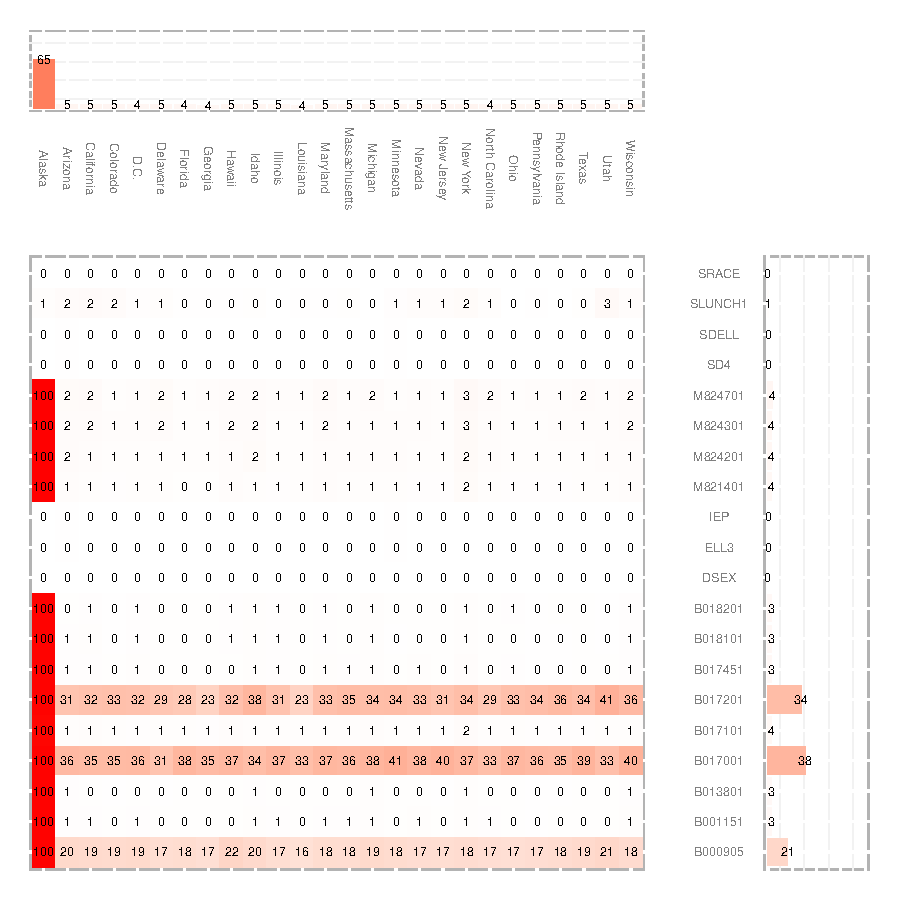
\includegraphics[width=\textwidth]{../Figures2009/g4math-missing.pdf}
\caption{Covariate missingness for grade 4 math}
\label{fig:g4math:missing}
\end{center}
\end{figure}

\begin{figure}[h]
\begin{center}
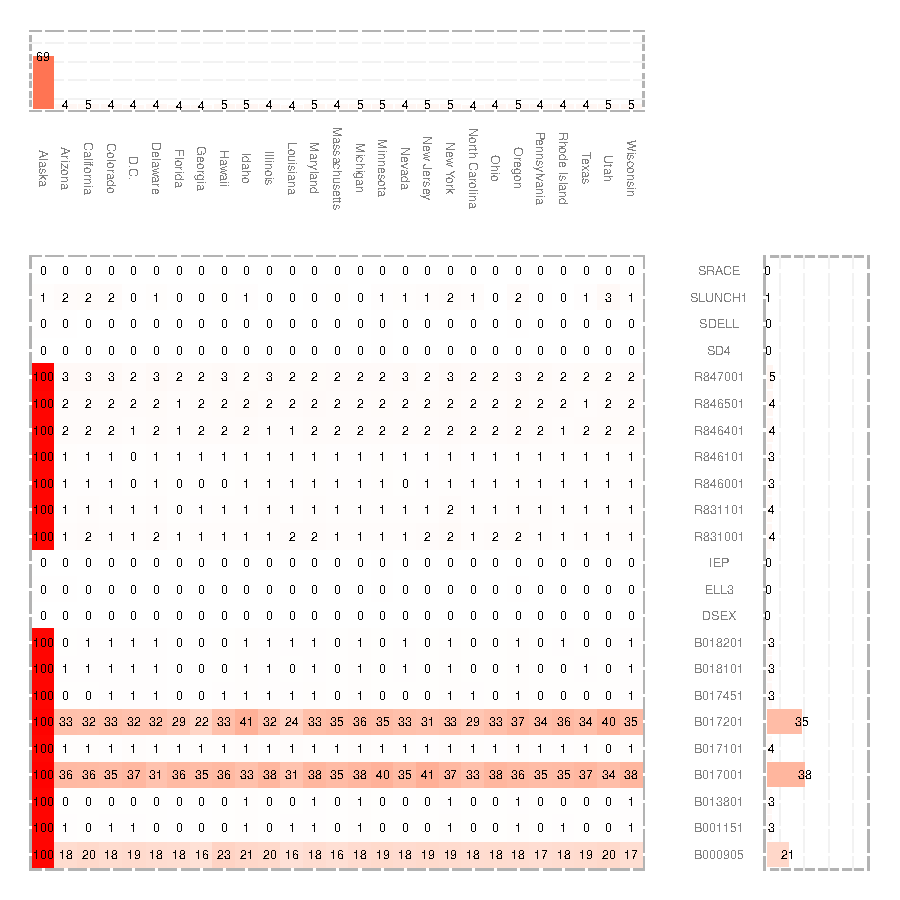
\includegraphics[width=\textwidth]{../Figures2009/g4read-missing.pdf}
\caption{Covariate missingness for grade 4 reading}
\label{fig:g4reading:missing}
\end{center}
\end{figure}

\begin{figure}[h]
\begin{center}
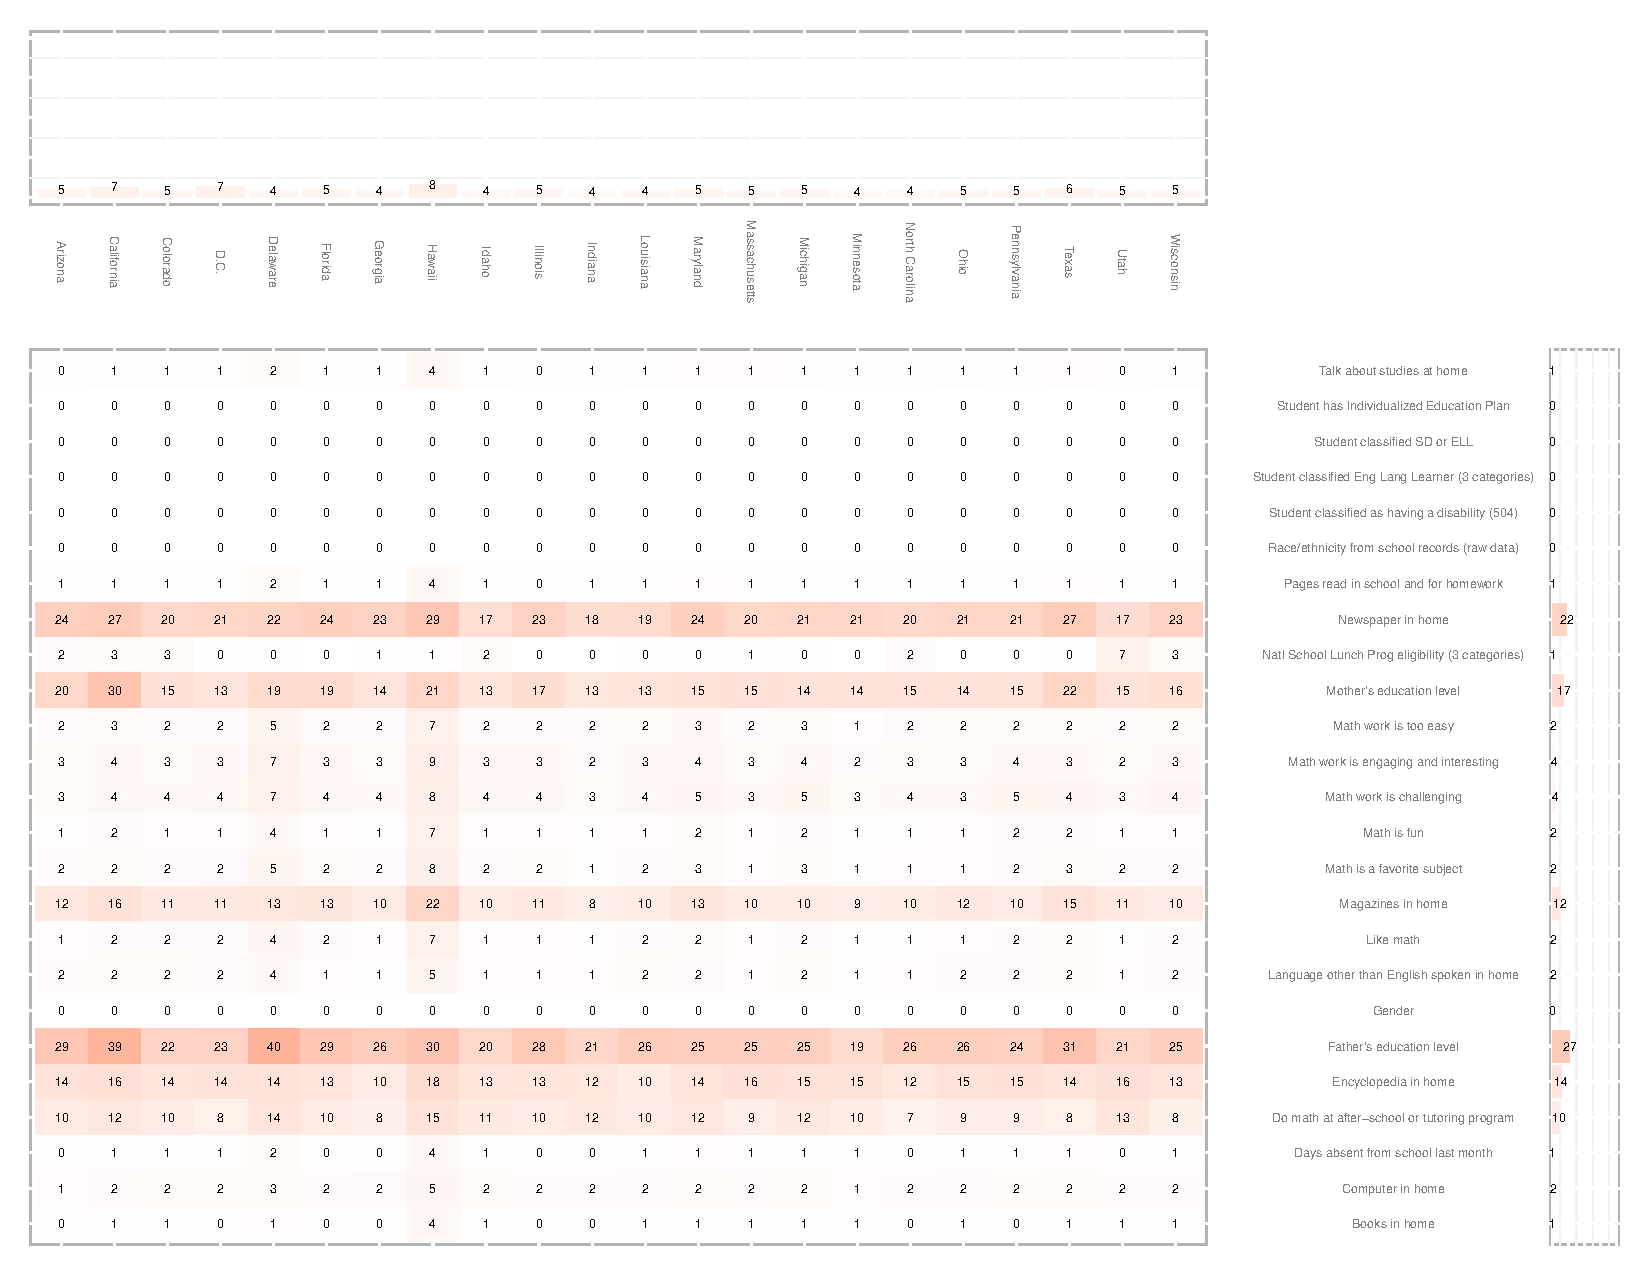
\includegraphics[width=\textwidth]{../Figures2009/g8math-missing.pdf}
\caption{Covariate missingness for grade 8 math}
\label{fig:g8math:missing}
\end{center}
\end{figure}

\begin{figure}[h]
\begin{center}
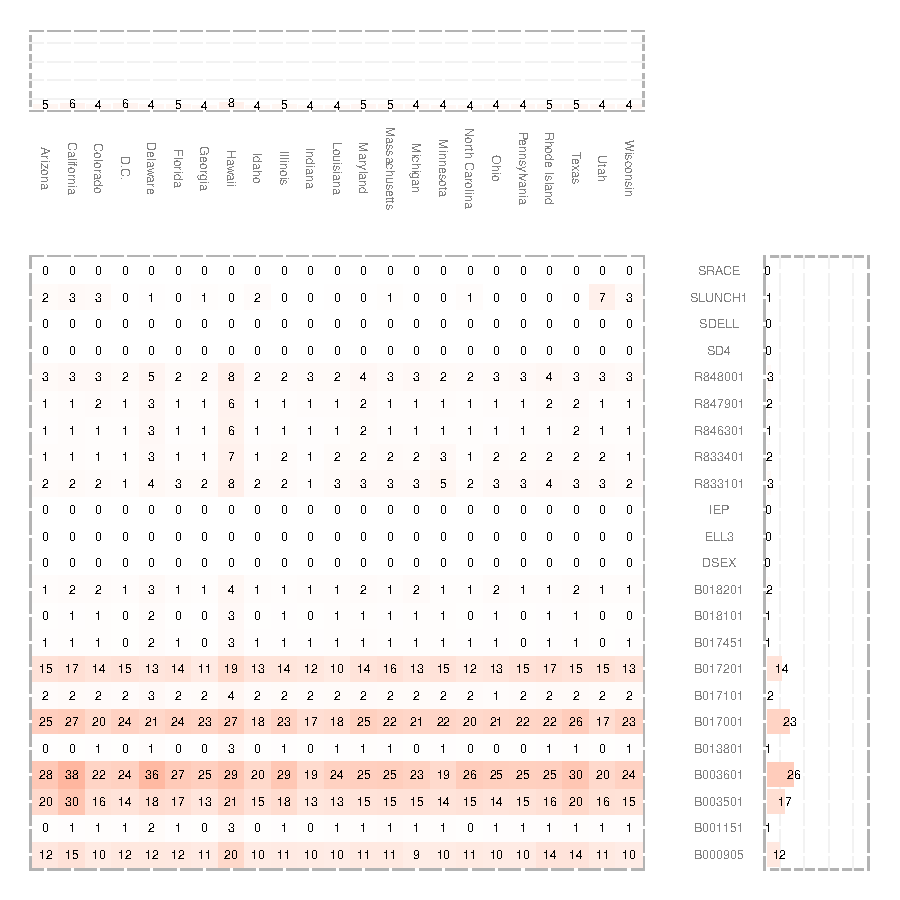
\includegraphics[width=\textwidth]{../Figures2009/g8read-missing.pdf}
\caption{Covariate missingness for grade 8 reading}
\label{fig:g8reading:missing}
\end{center}
\end{figure}


%==================== Appendix D ====================================================================
\clearpage
\addcontentsline{toc}{subsection}{Appendix D: Loess Regression Plots}
\section*{Appendix D\\Loess Regression Plots}
\label{appendixD}

\begin{figure}[h!]
\begin{center}
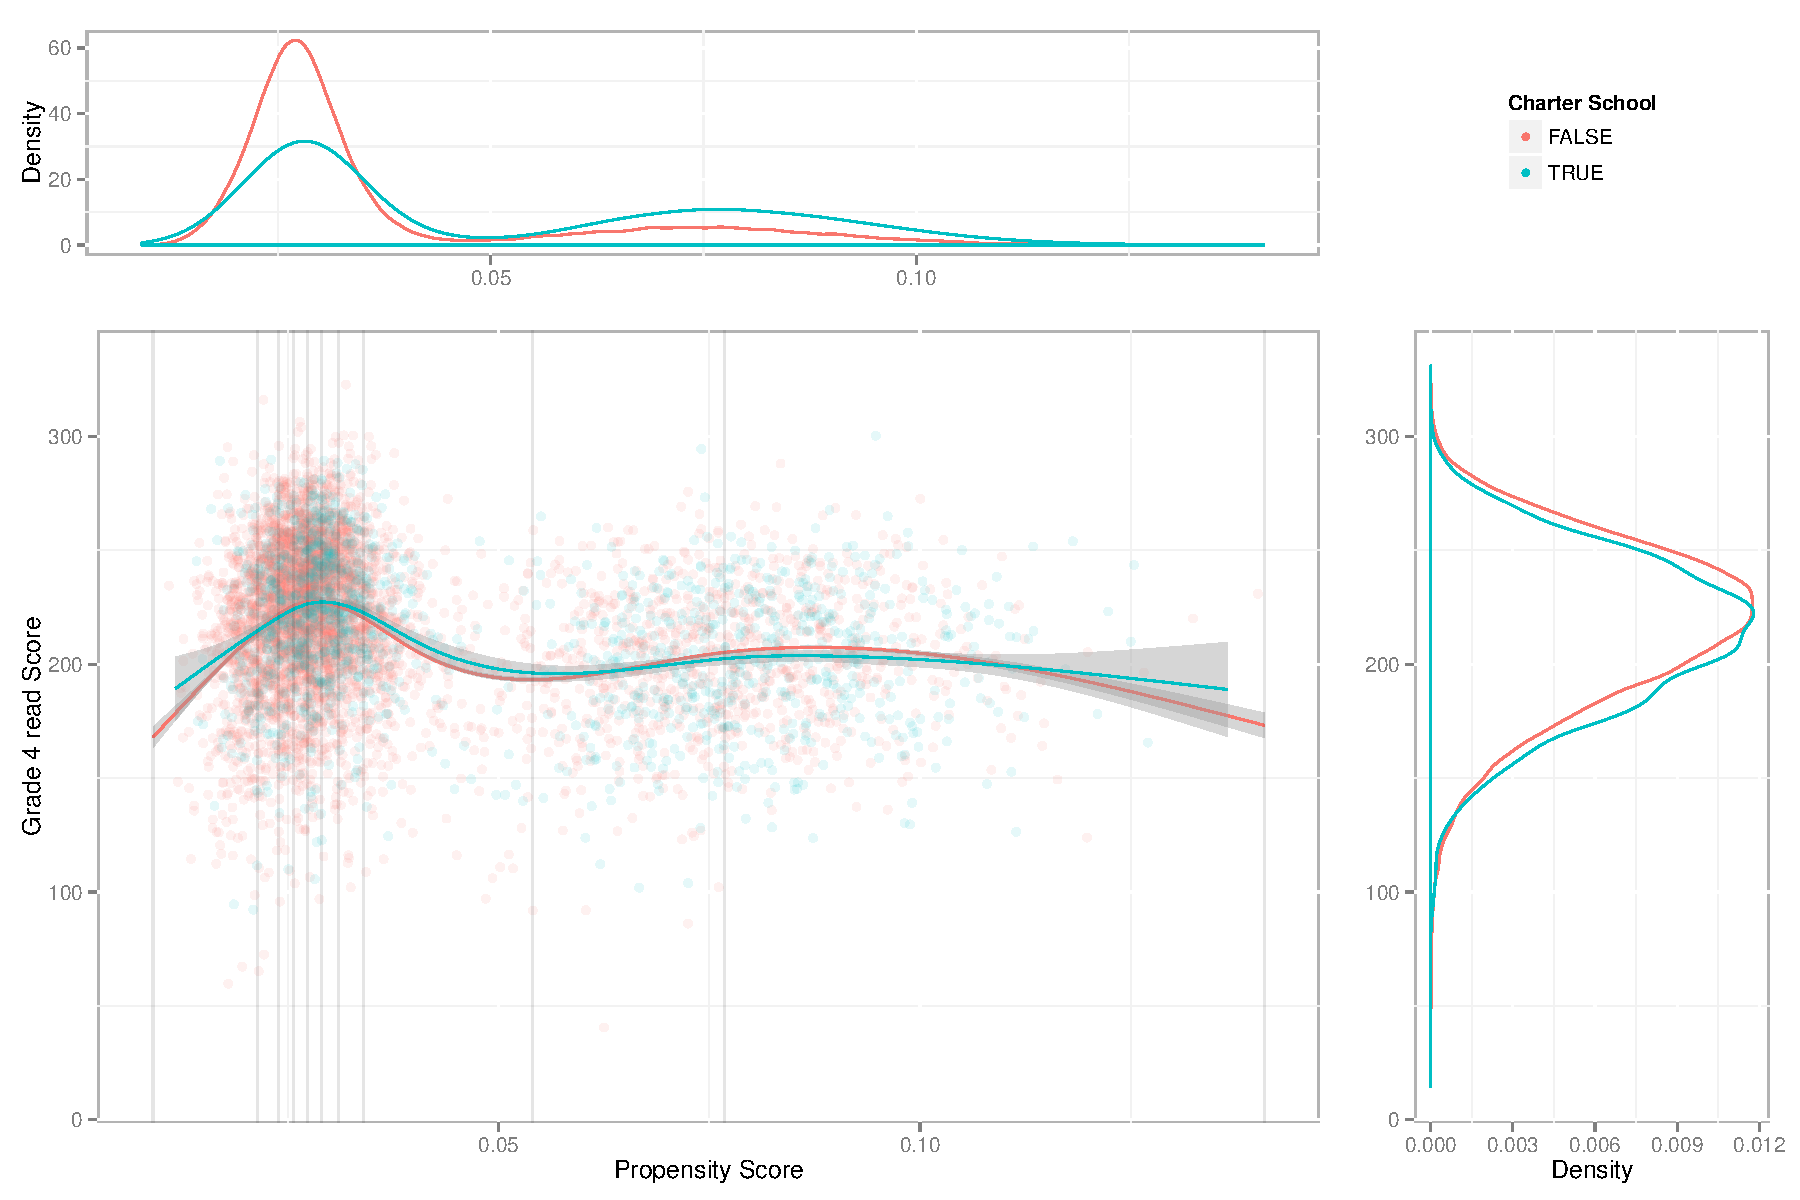
\includegraphics[height=.4\textheight]{../Figures2009/g4read-loess.pdf}
\caption{Loess regression assessment plot: Grade 4 reading}
\label{fig:g4read:loess}
\end{center}
\end{figure}

\begin{figure}[h!]
\begin{center}
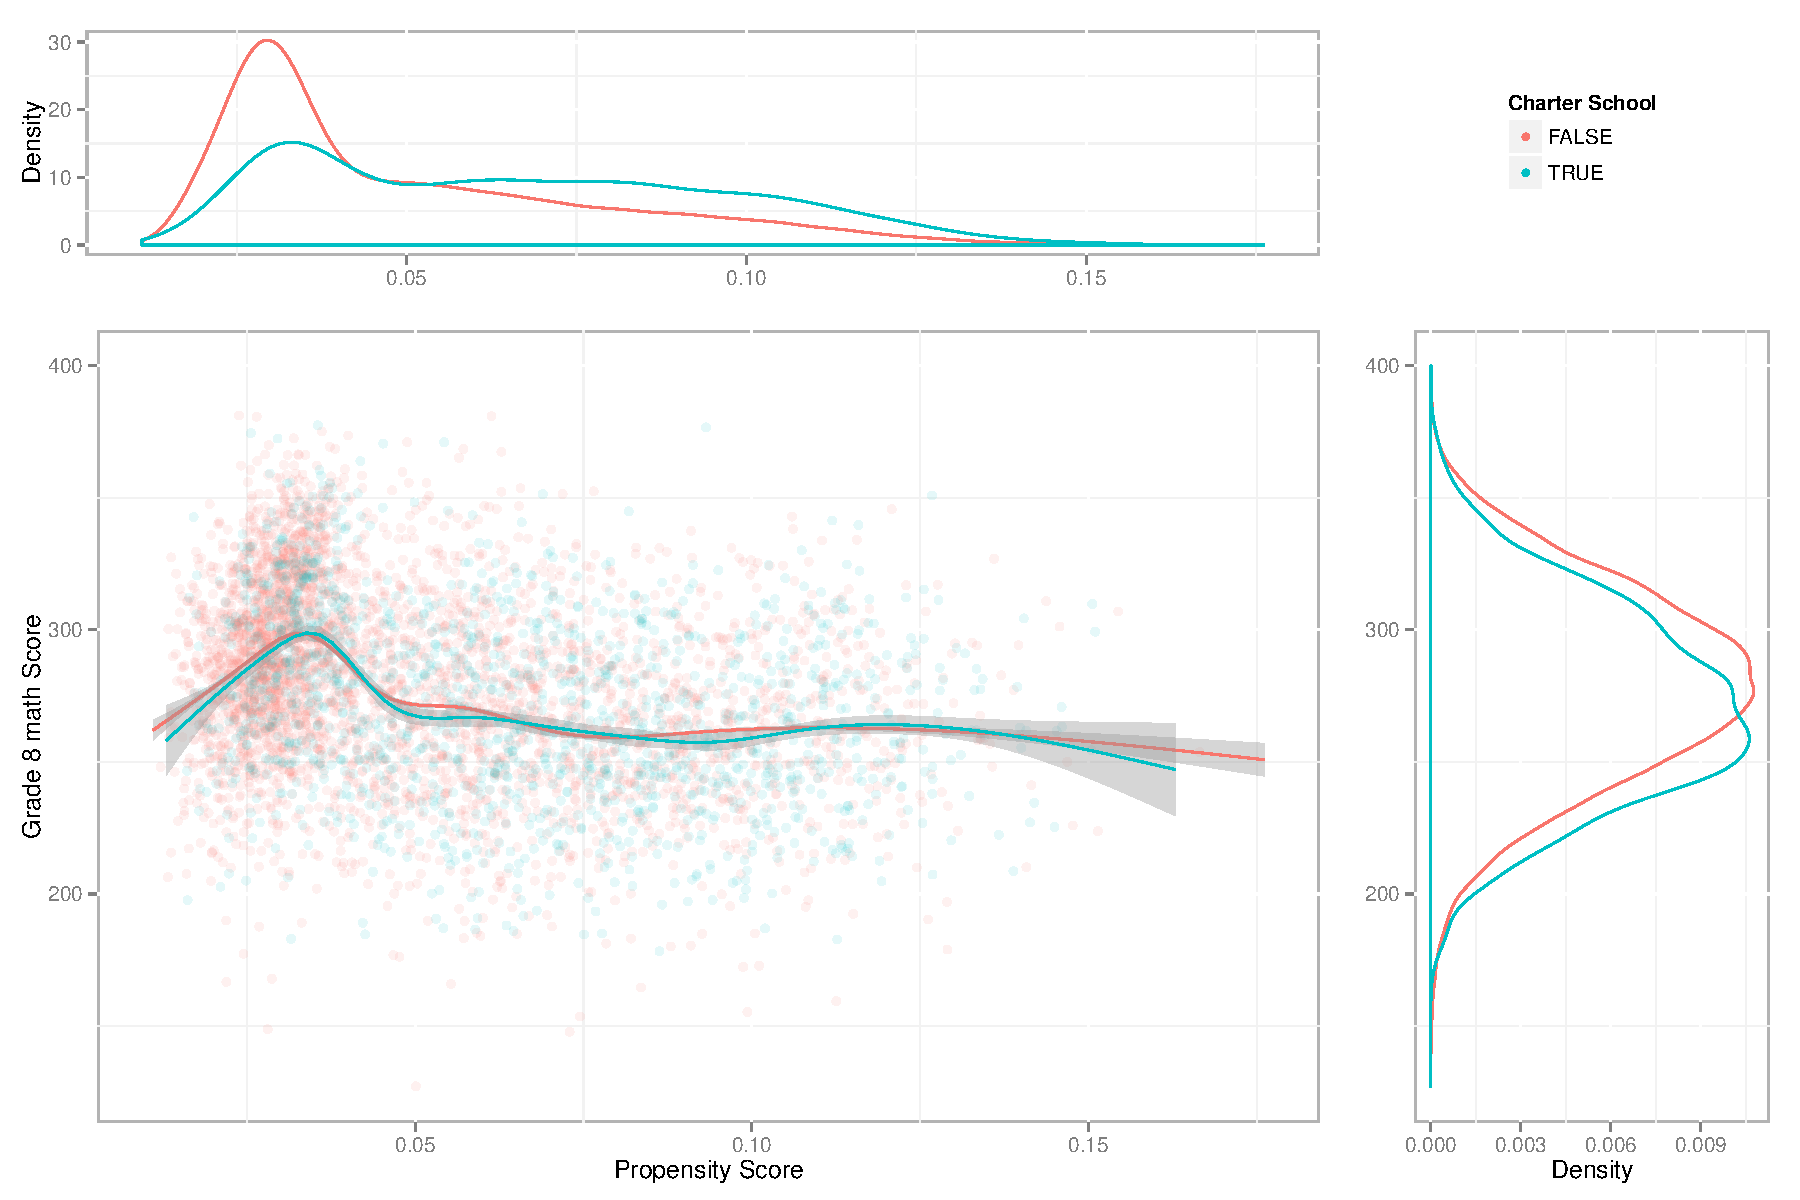
\includegraphics[height=.4\textheight]{../Figures2009/g8math-loess.pdf}
\caption{Loess regression assessment plot: Grade 8 math}
\label{fig:g8math:loess}
\end{center}
\end{figure}

\begin{figure}[h!]
\begin{center}
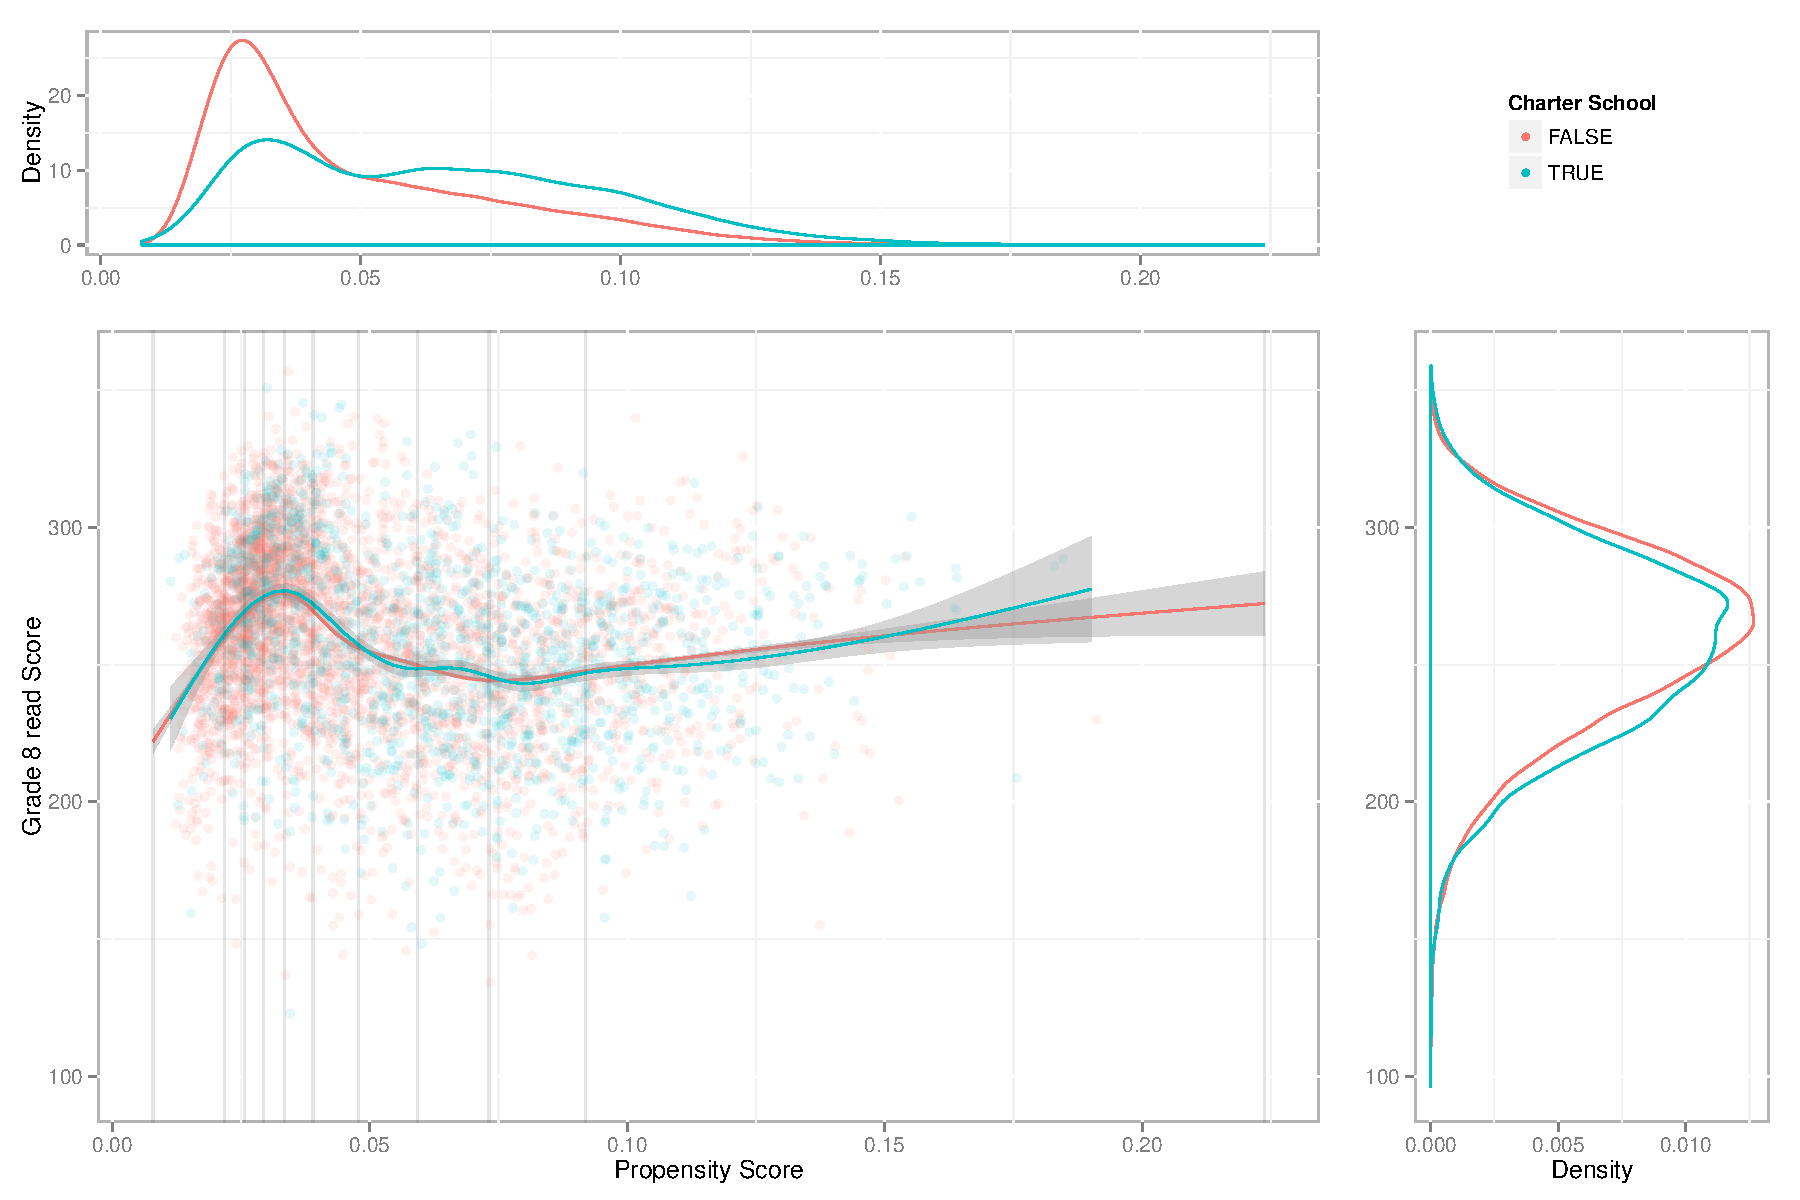
\includegraphics[height=.4\textheight]{../Figures2009/g8read-loess.pdf}
\caption{Loess regression assessment plot: Grade 8 reading}
\label{fig:g8read:loess}
\end{center}
\end{figure}

\begin{figure}[h!]
\begin{center}
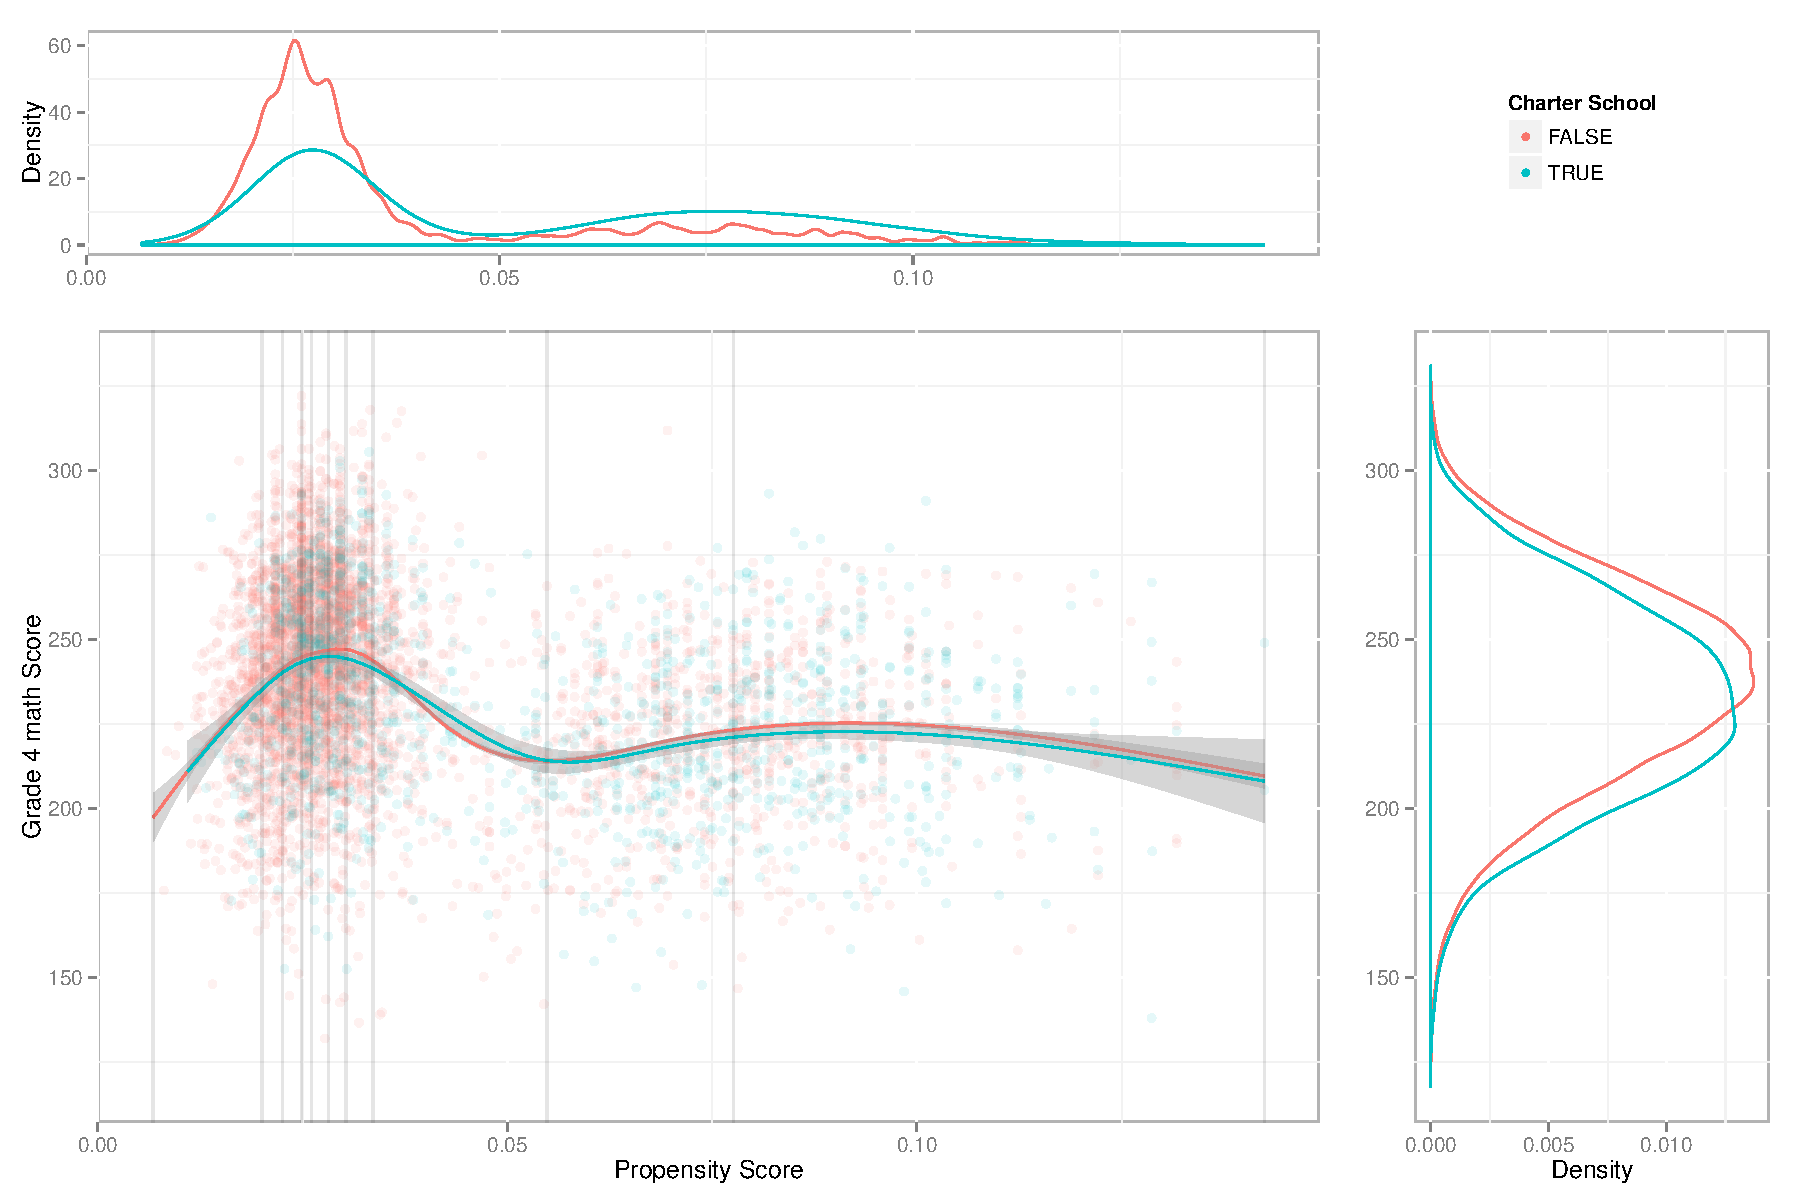
\includegraphics[height=.4\textheight]{../Figures2009/g4math-loessAIC.pdf}
\caption{Loess regression AIC assessment plot: Grade 4 math}
\label{fig:g4math:loessAIC}
\end{center}
\end{figure}

\begin{figure}[h!]
\begin{center}
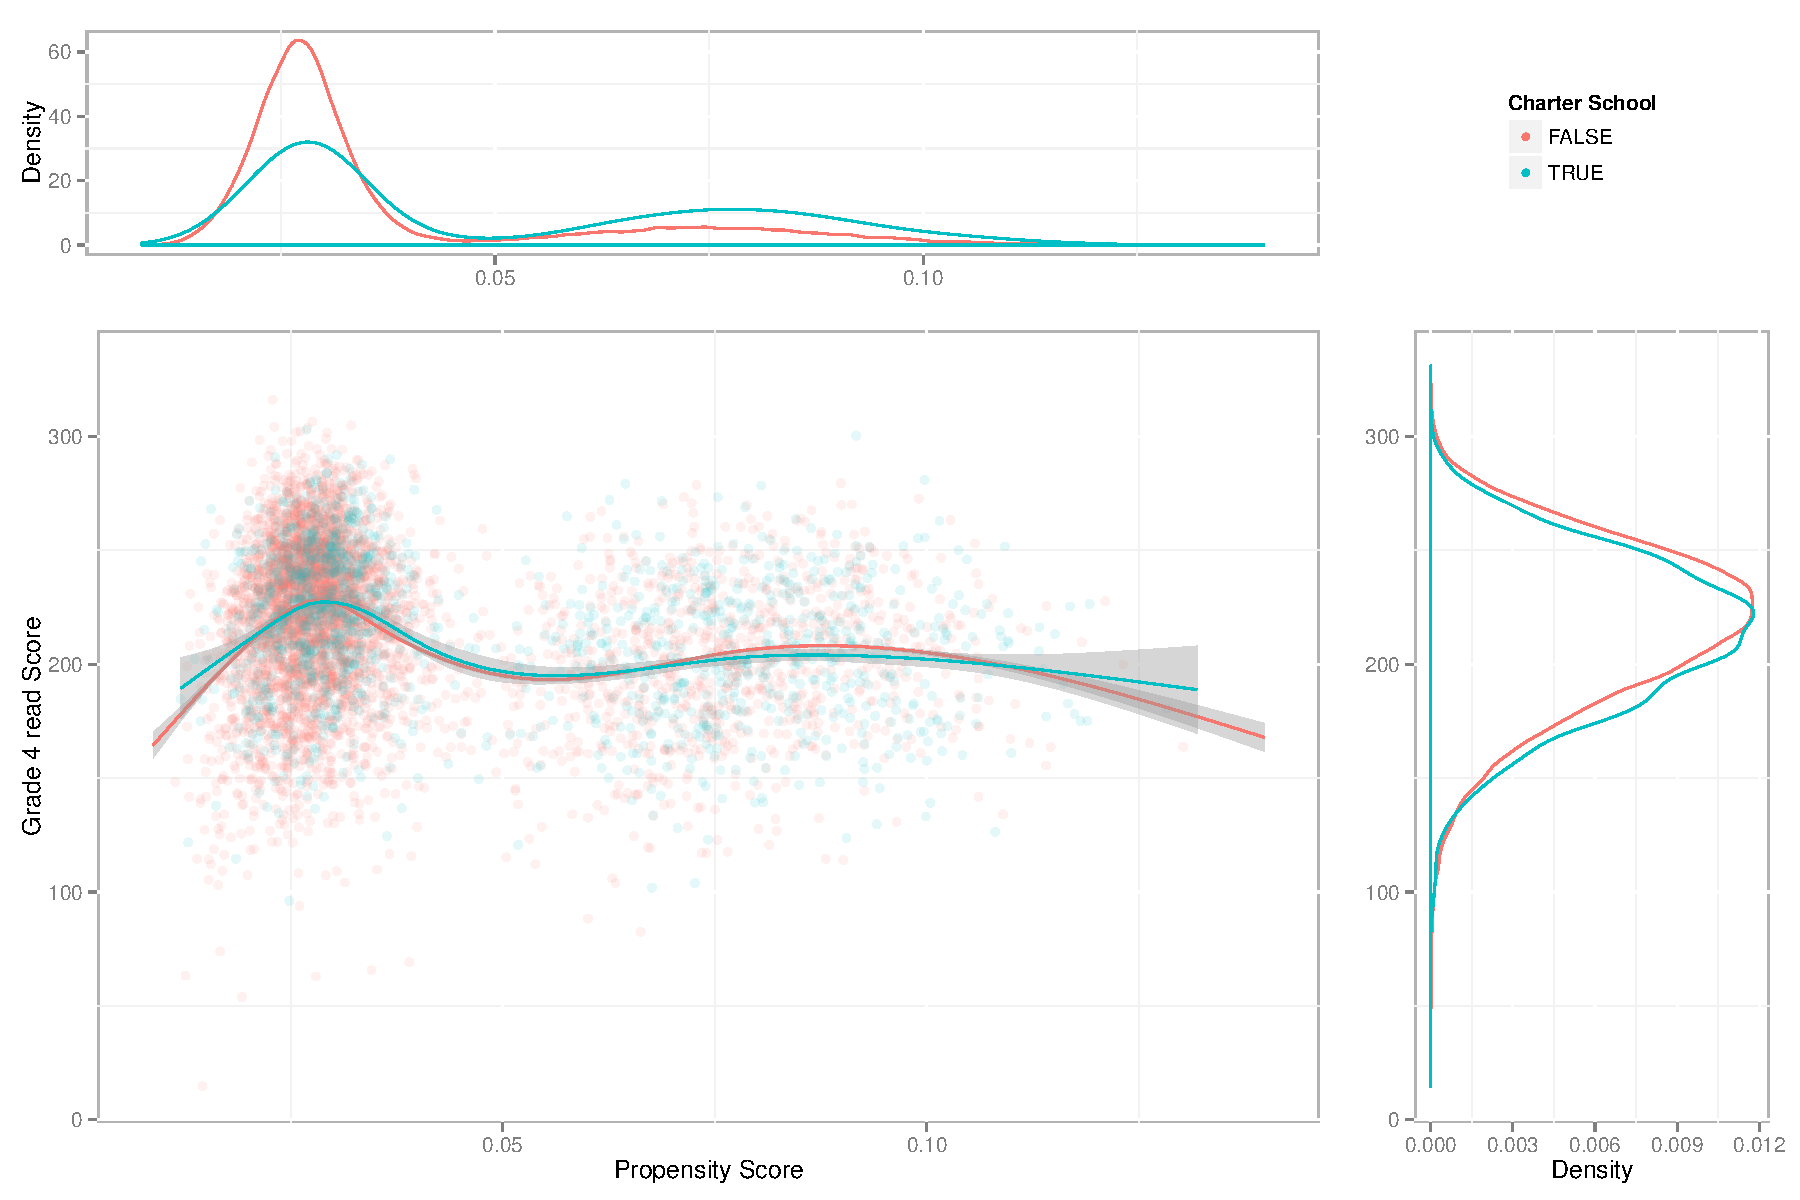
\includegraphics[height=.4\textheight]{../Figures2009/g4read-loessAIC.pdf}
\caption{Loess regression AIC assessment plot: Grade 4 reading}
\label{fig:g4read:loess}
\end{center}
\end{figure}

\begin{figure}[h!]
\begin{center}
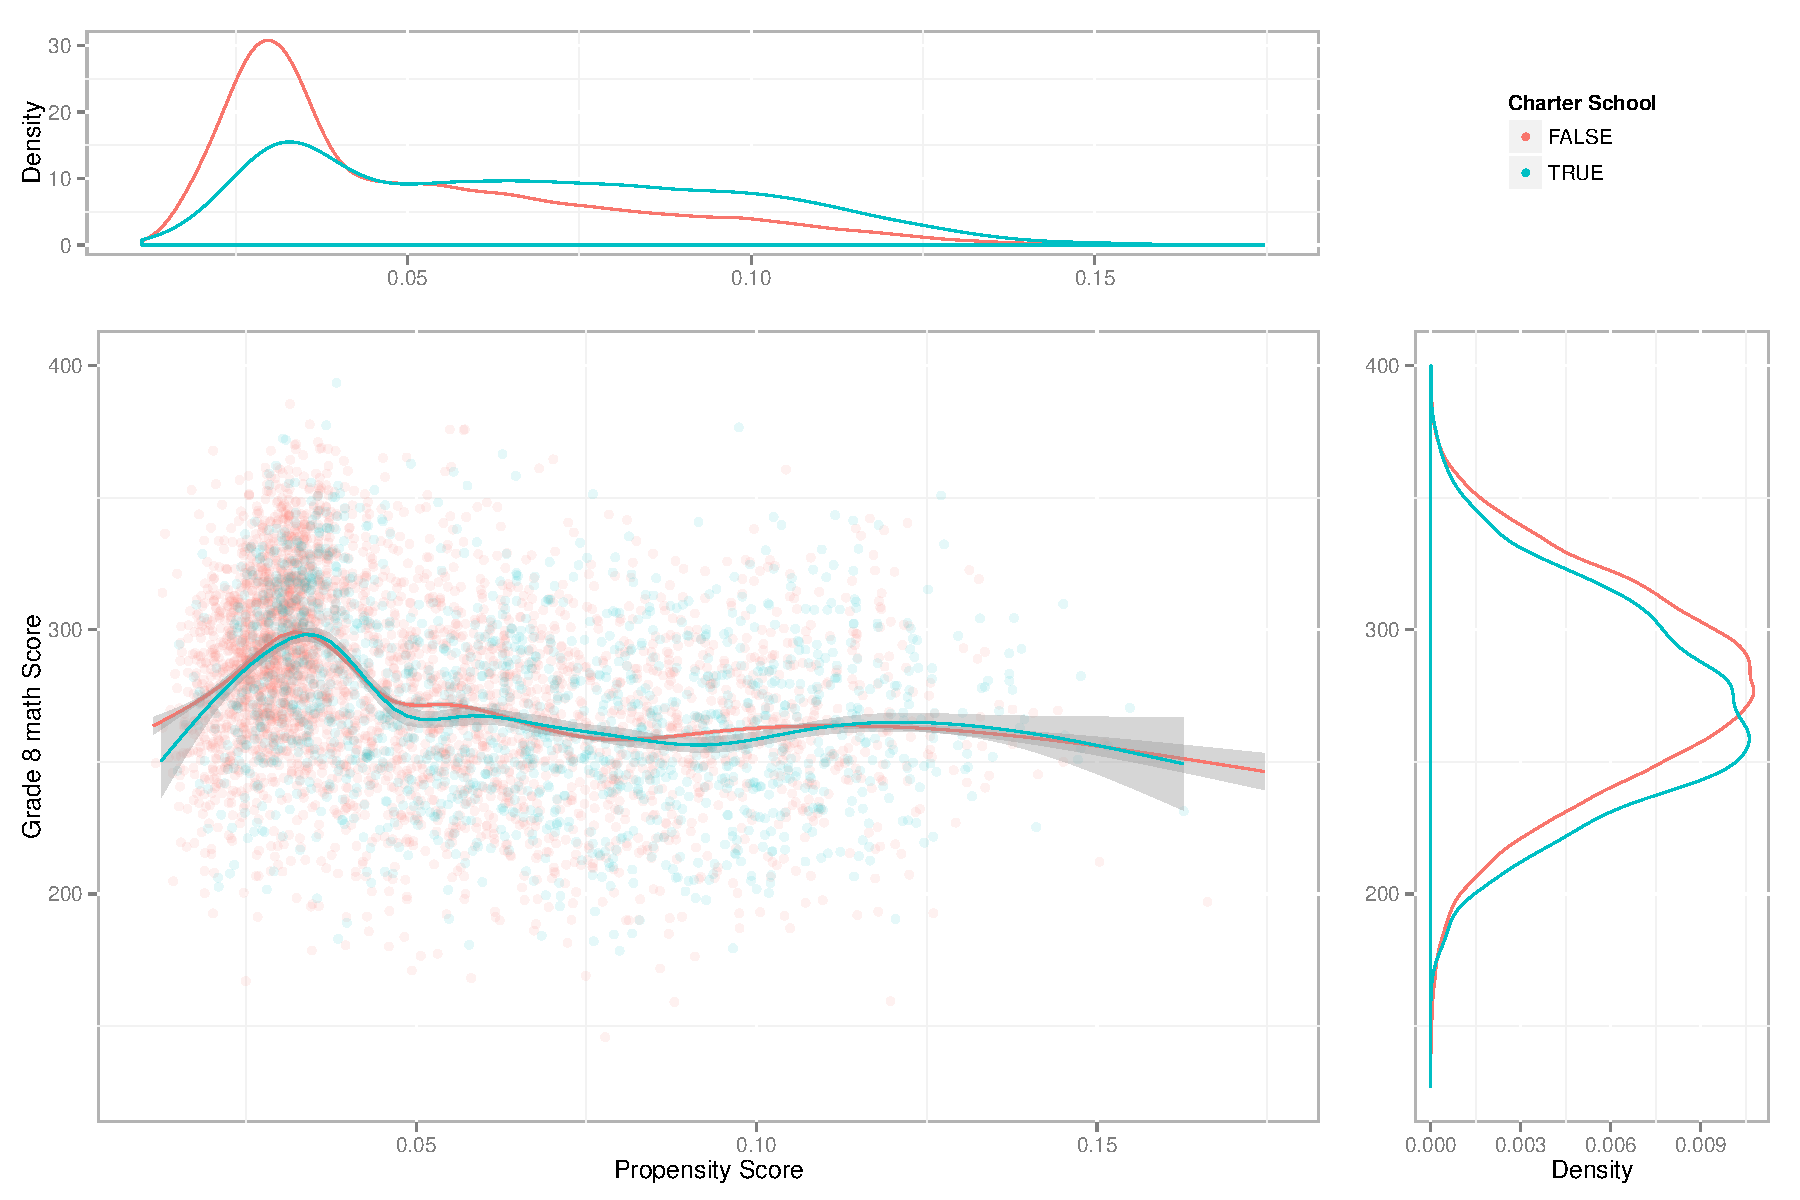
\includegraphics[height=.4\textheight]{../Figures2009/g8math-loessAIC.pdf}
\caption{Loess regression AIC assessment plot: Grade 8 math}
\label{fig:g8math:loess}
\end{center}
\end{figure}

\begin{figure}[h!]
\begin{center}
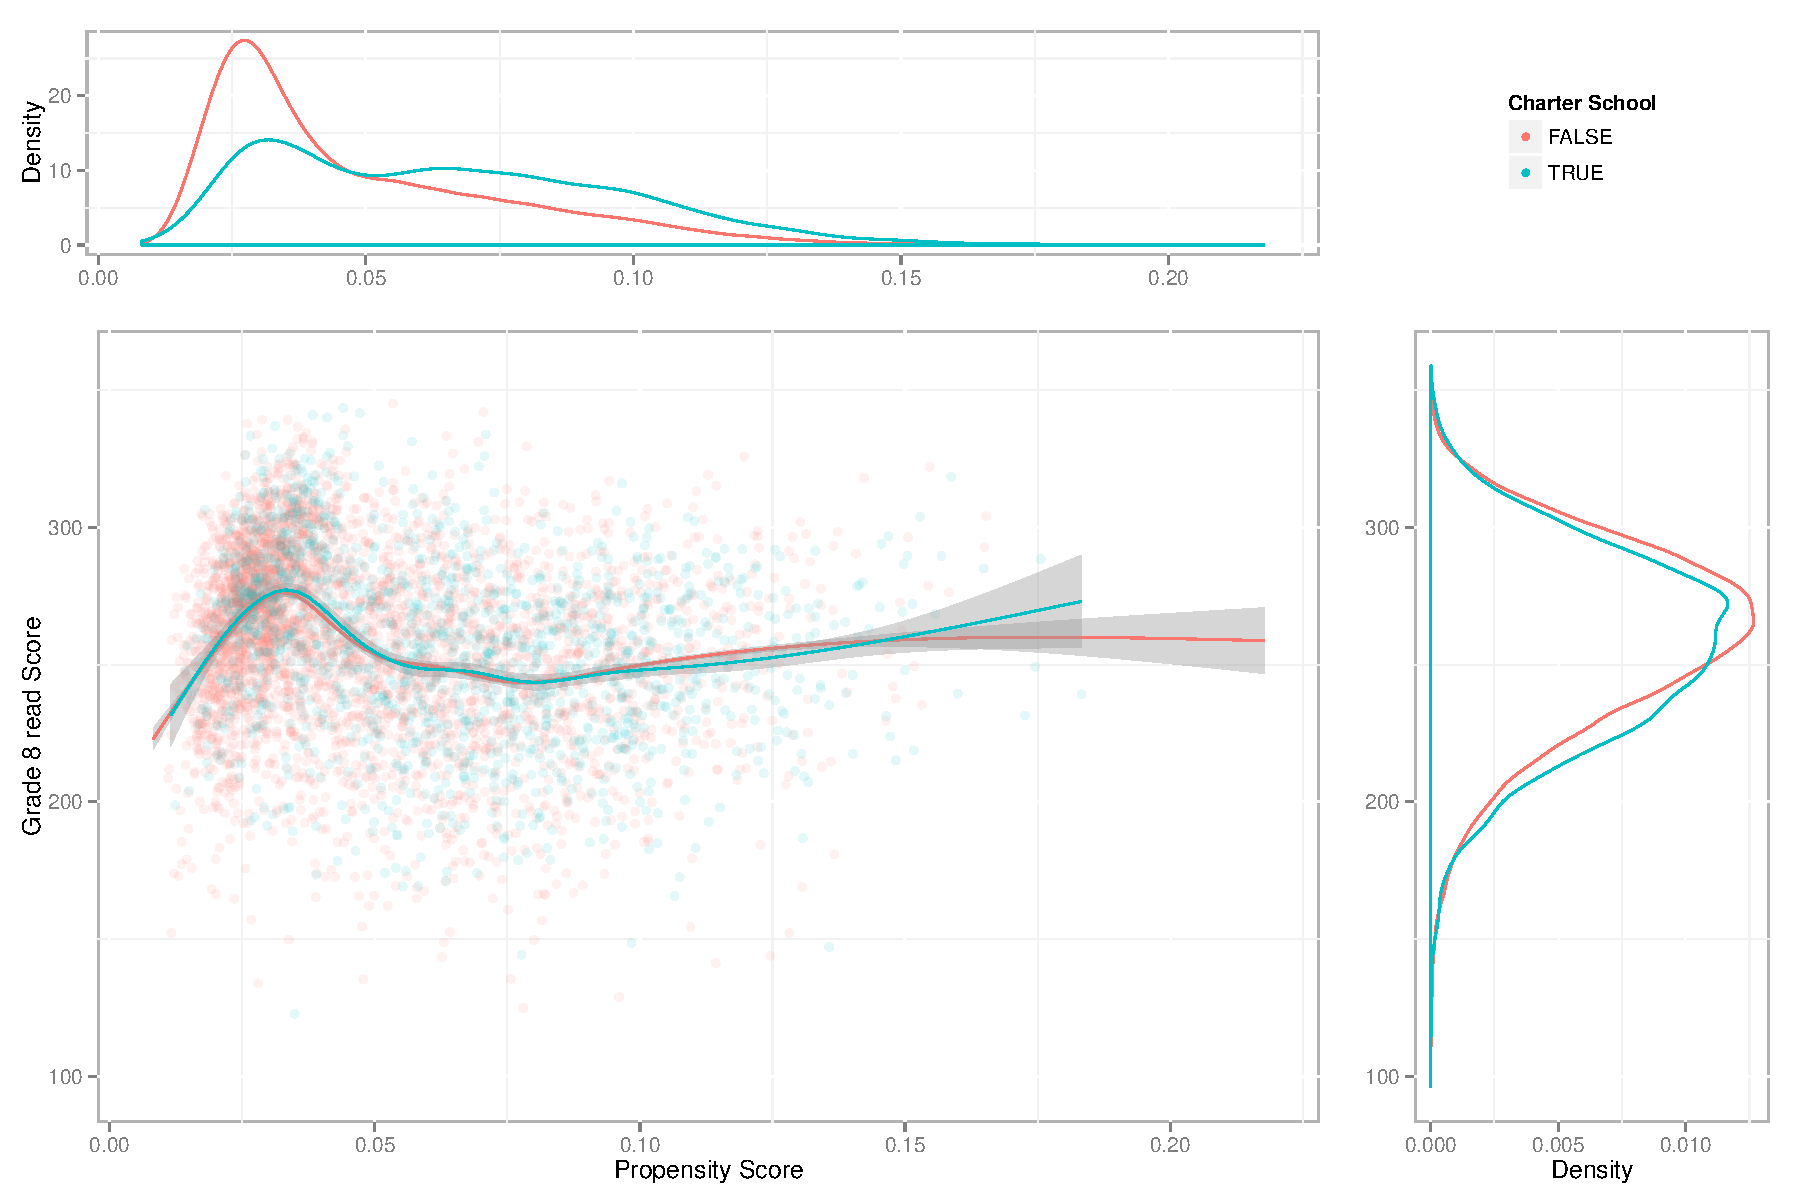
\includegraphics[height=.4\textheight]{../Figures2009/g8read-loessAIC.pdf}
\caption{Loess regression AIC assessment plot: Grade 8 reading}
\label{fig:g8read:loess}
\end{center}
\end{figure}


%==================== Appendix E ====================================================================
\clearpage
\addcontentsline{toc}{subsection}{Appendix E: Covariate Balance Plots}
\section*{Appendix E\\Covariate Balance Plots}
\label{appendixE}

% Grade 4 math

\begin{figure}[h!]
\begin{center}
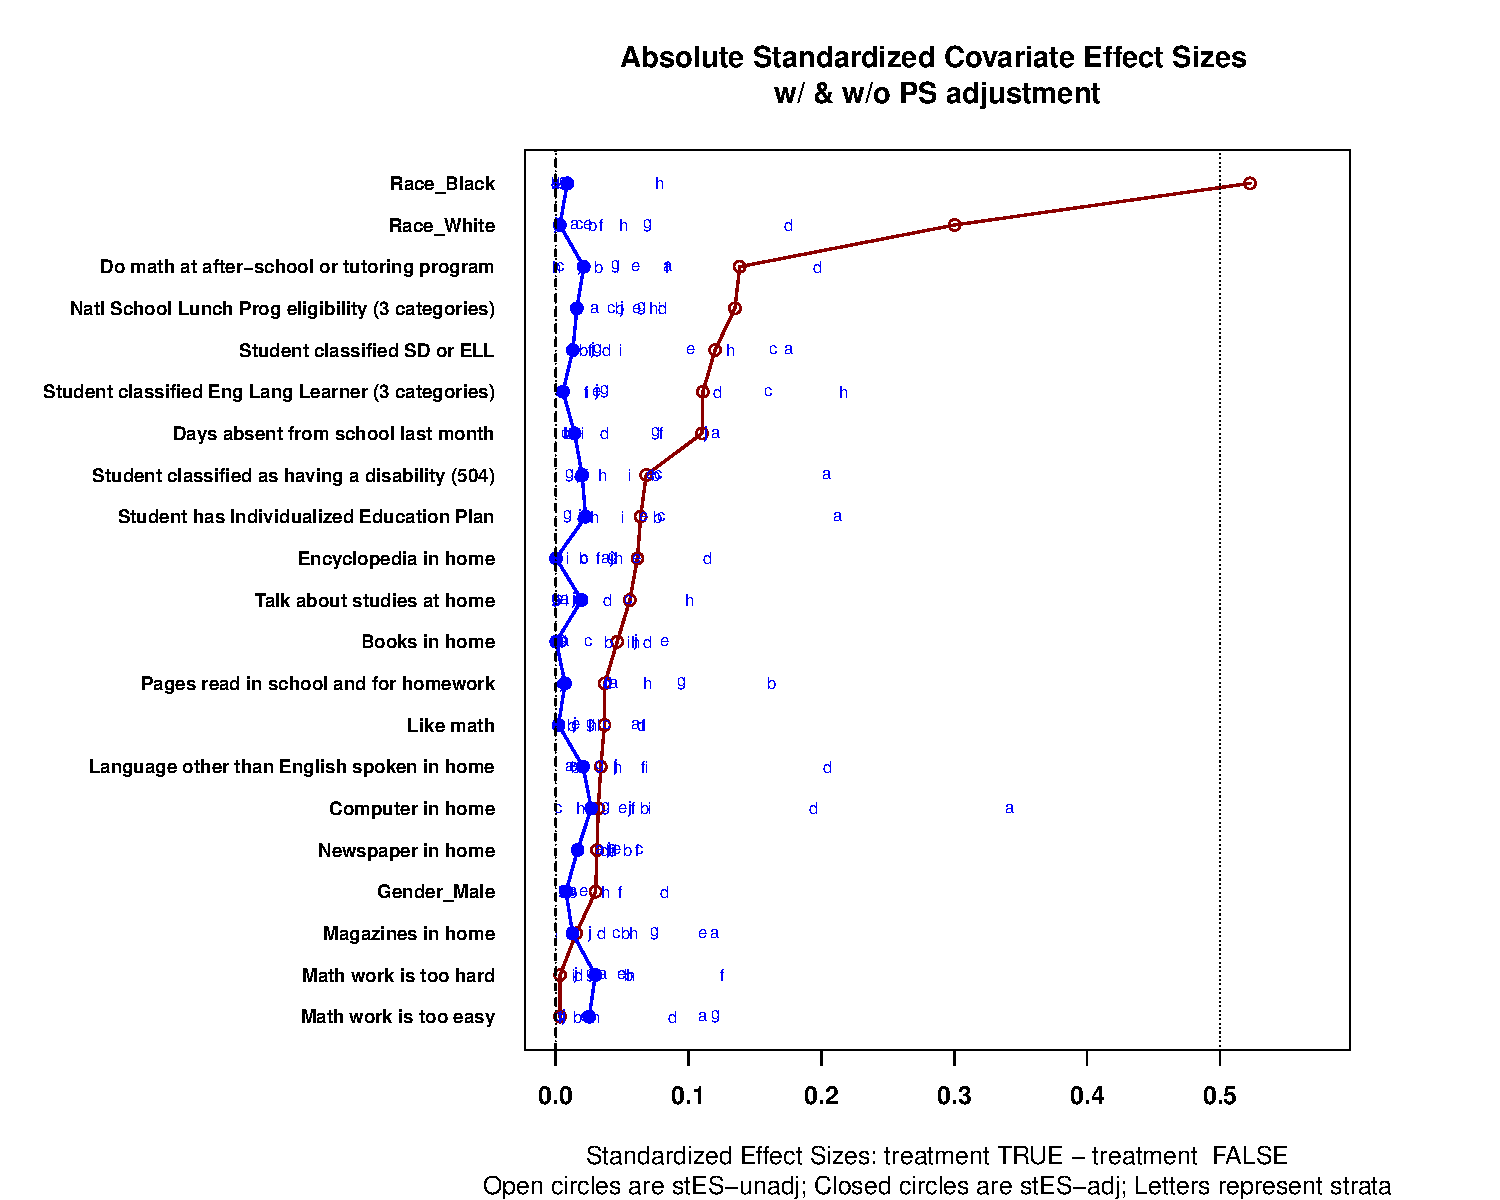
\includegraphics[width=\textwidth]{../Figures2009/g4math-lrAIC-balance.pdf}
\caption{Covariate balance plot for logistic regression AIC stratification: Grade 4 math}
\end{center}
\end{figure}

\begin{figure}
\begin{center}
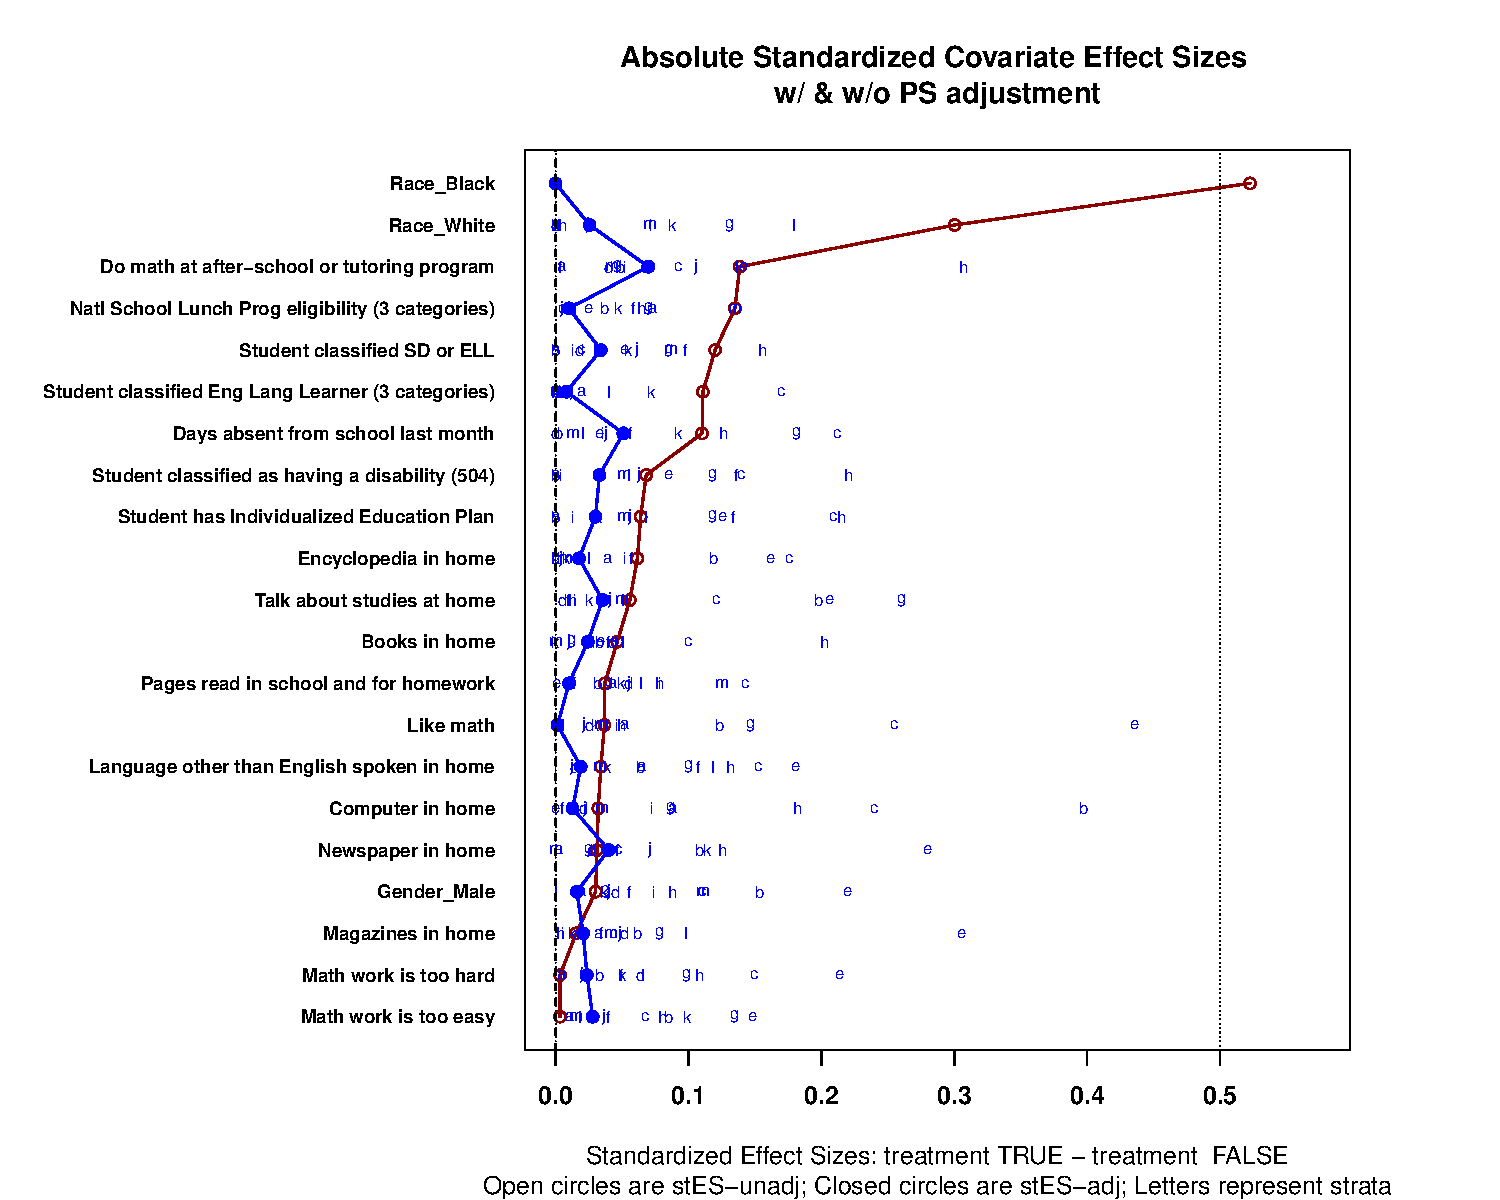
\includegraphics[width=\textwidth]{../Figures2009/g4math-tree-balance.pdf}
\caption{Covariate balance plot for classification tree stratification: Grade 4 math}
\end{center}
\end{figure}

% Grade 4 reading
\begin{figure}
\begin{center}
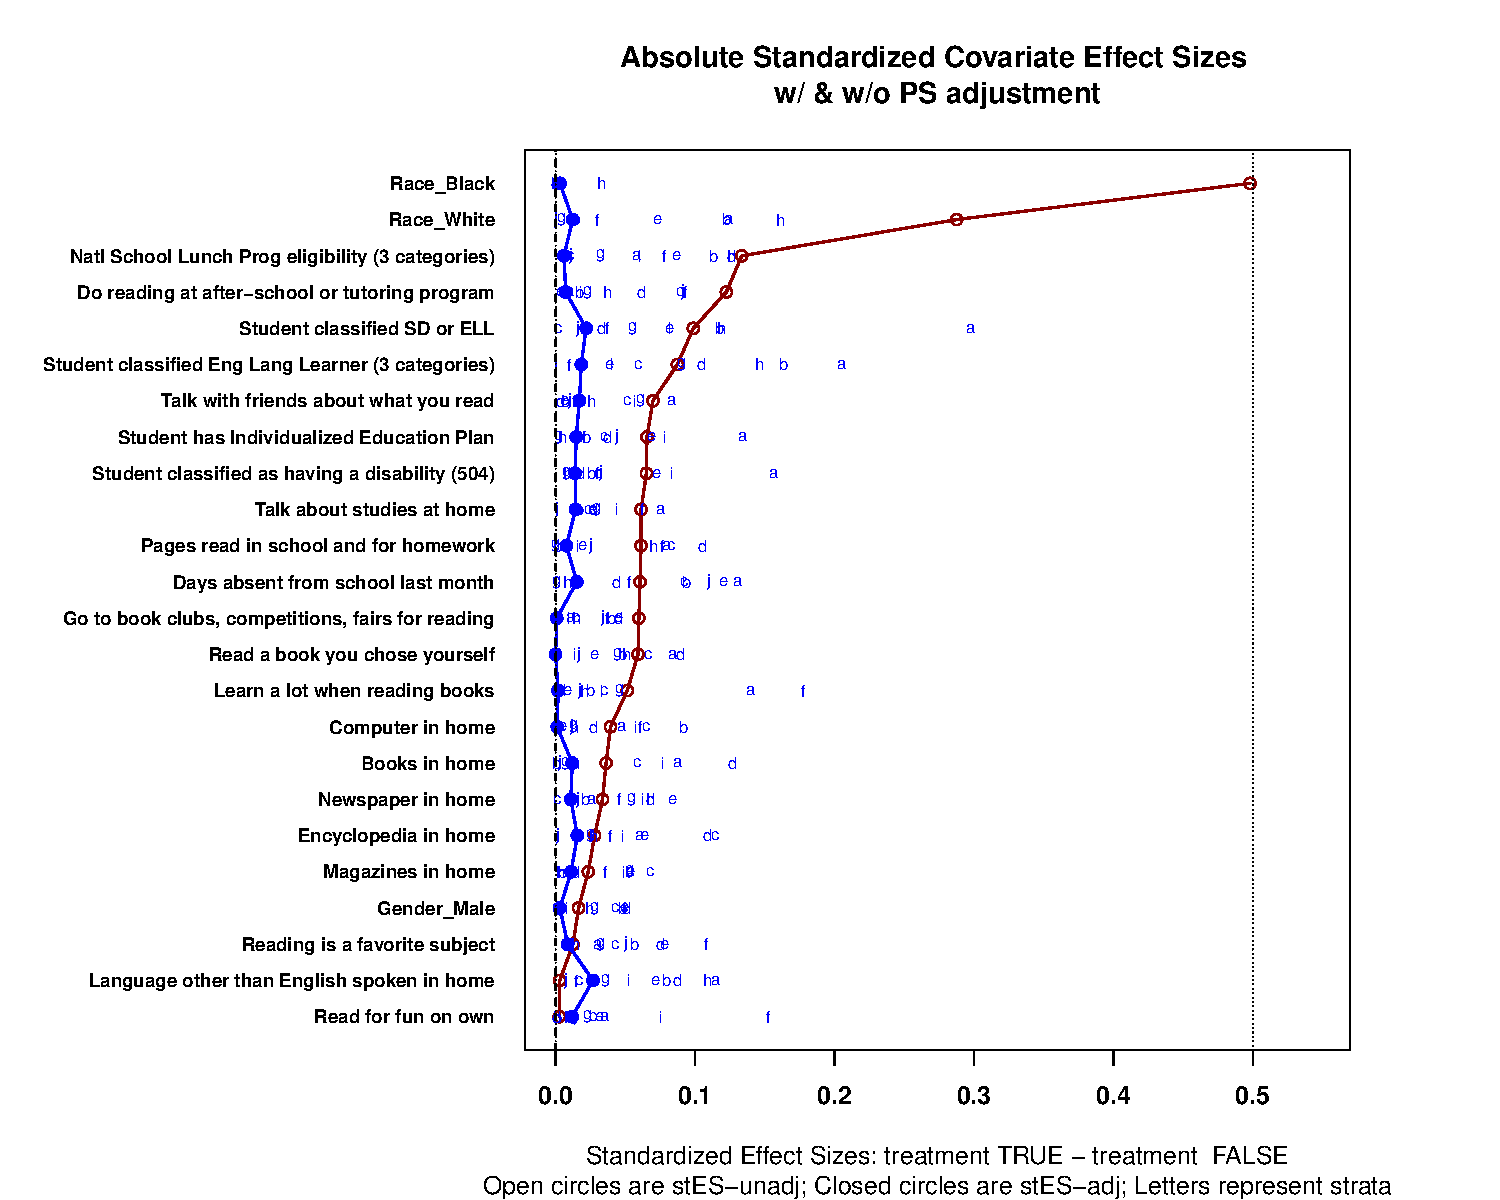
\includegraphics[width=\textwidth]{../Figures2009/g4read-lr-balance.pdf}
\caption{Covariate balance plot for logistic regression stratification: Grade 4 reading}
\end{center}
\end{figure}

\begin{figure}
\begin{center}
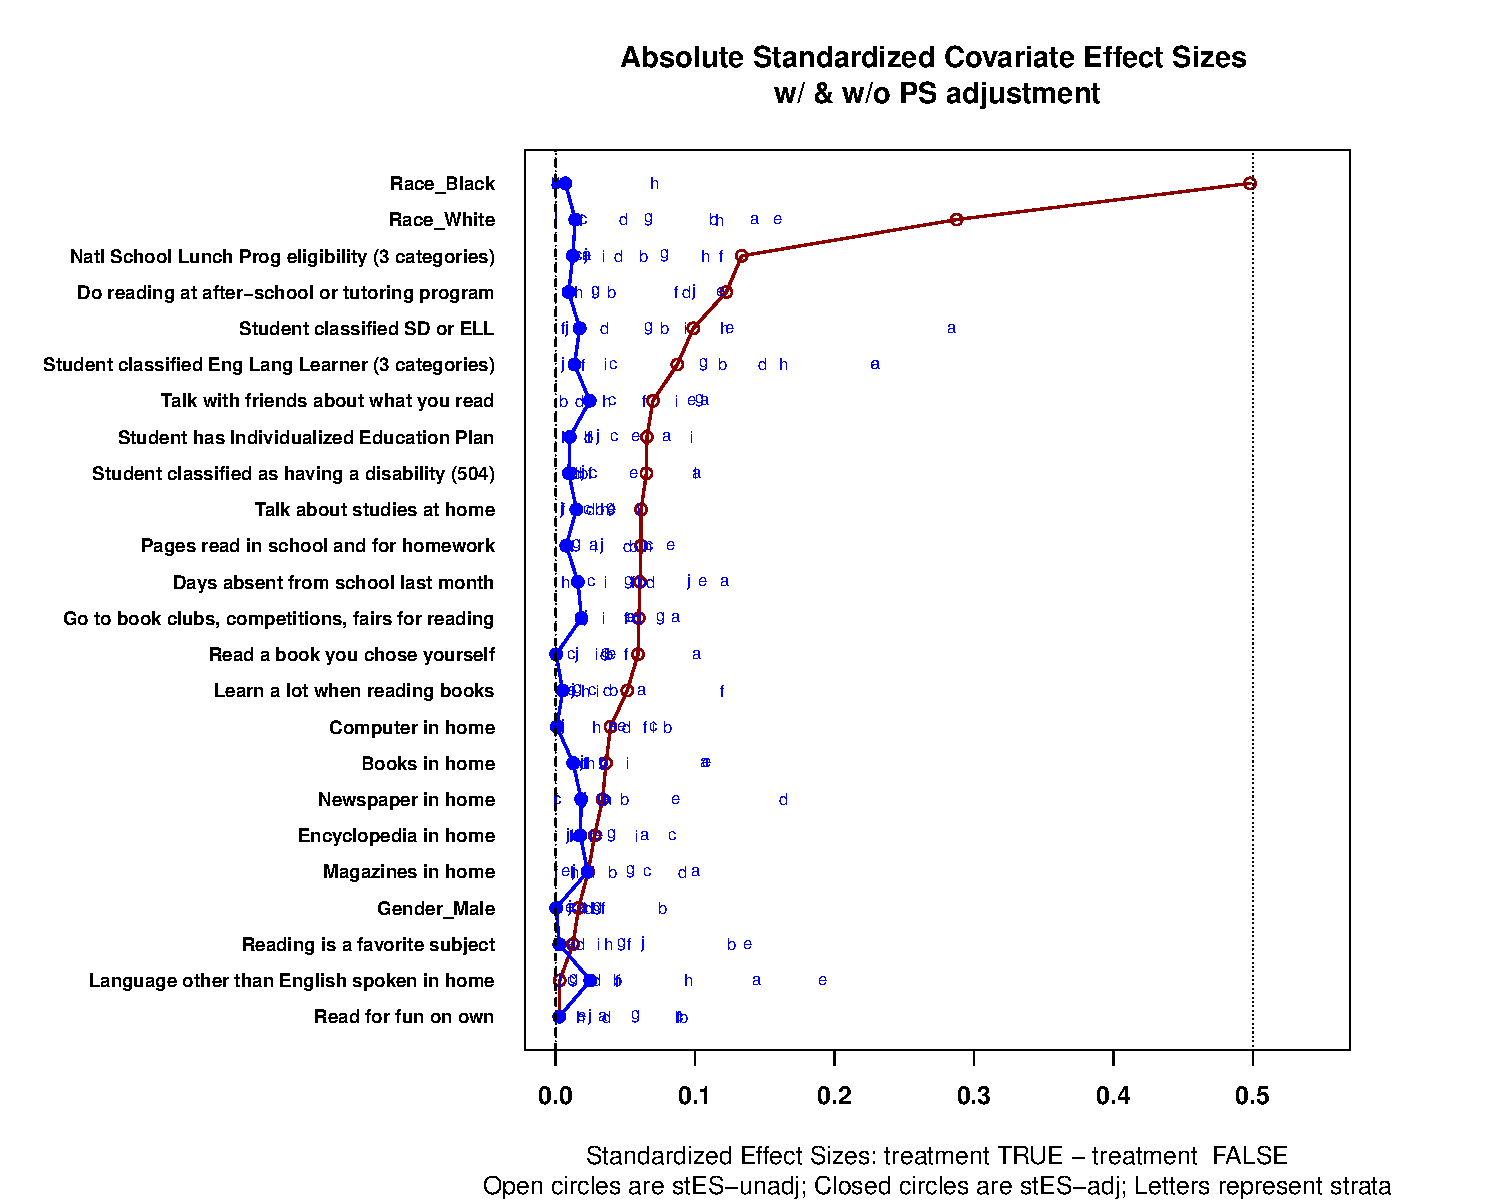
\includegraphics[width=\textwidth]{../Figures2009/g4read-lrAIC-balance.pdf}
\caption{Covariate balance plot for logistic regression AIC stratification: Grade 4 reading}
\end{center}
\end{figure}

\begin{figure}
\begin{center}
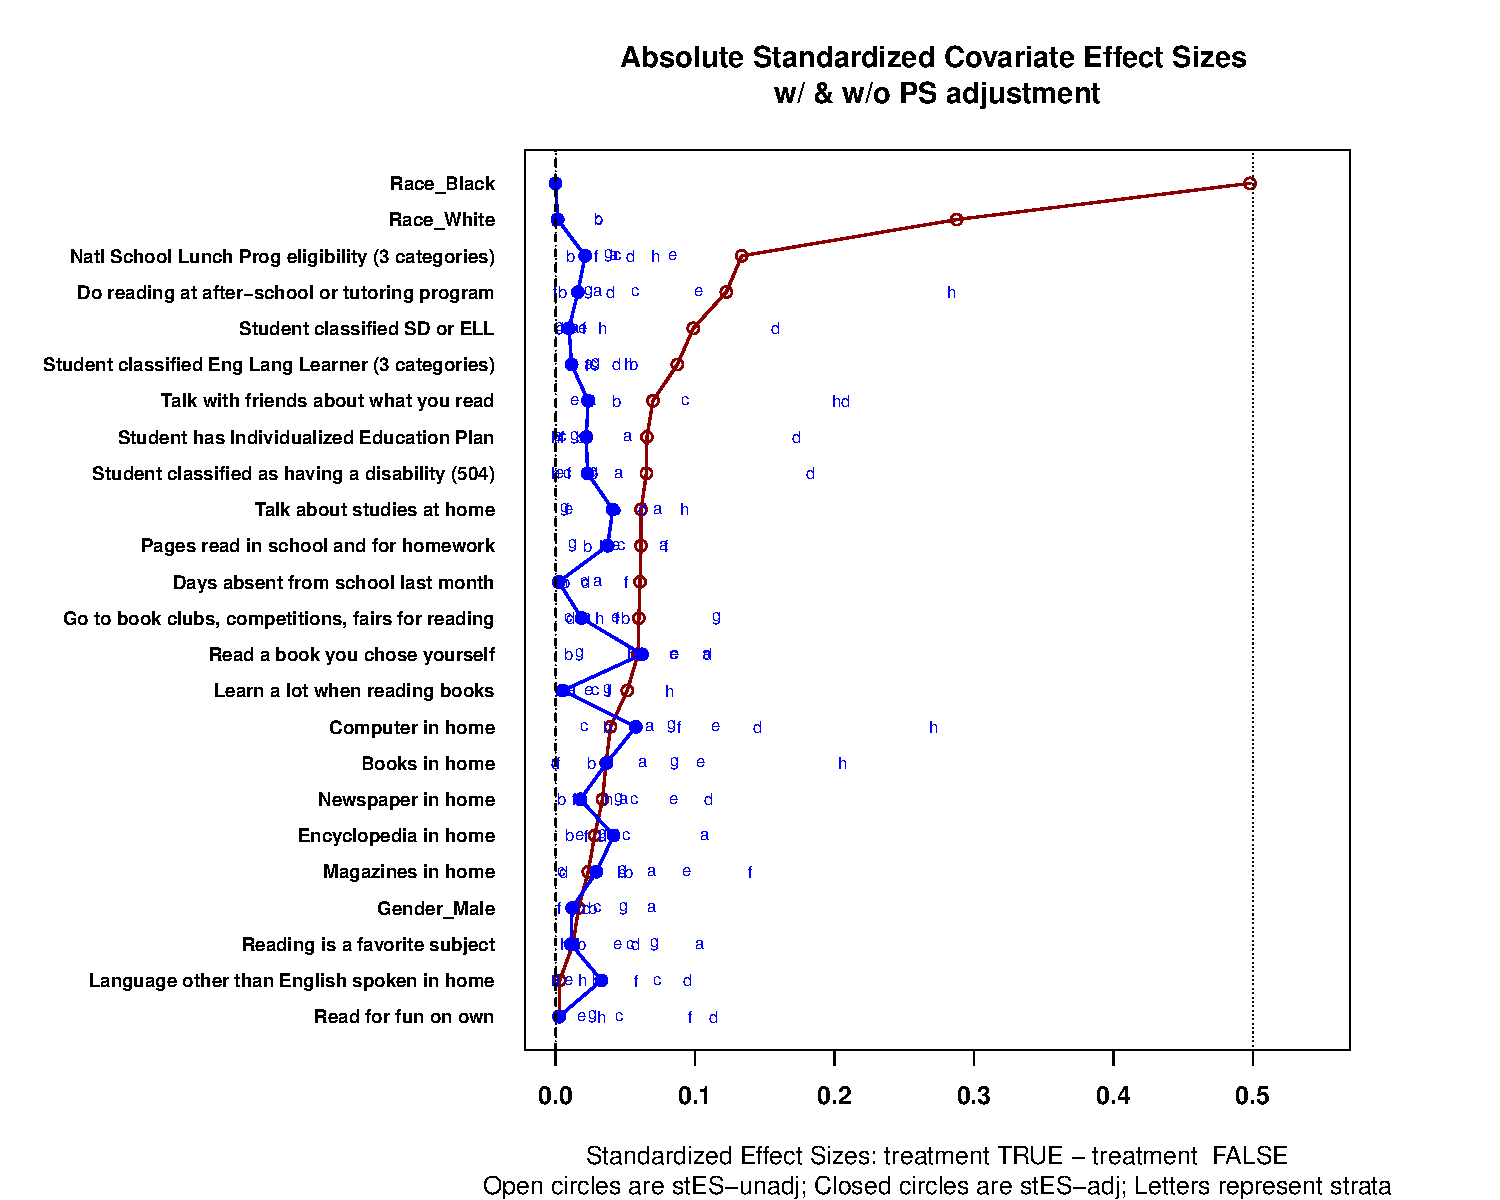
\includegraphics[width=\textwidth]{../Figures2009/g4read-tree-balance.pdf}
\caption{Covariate balance plot for classification tree stratification: Grade 4 reading}
\end{center}
\end{figure}

% Grade 8 math
\begin{figure}[h!]
\begin{center}
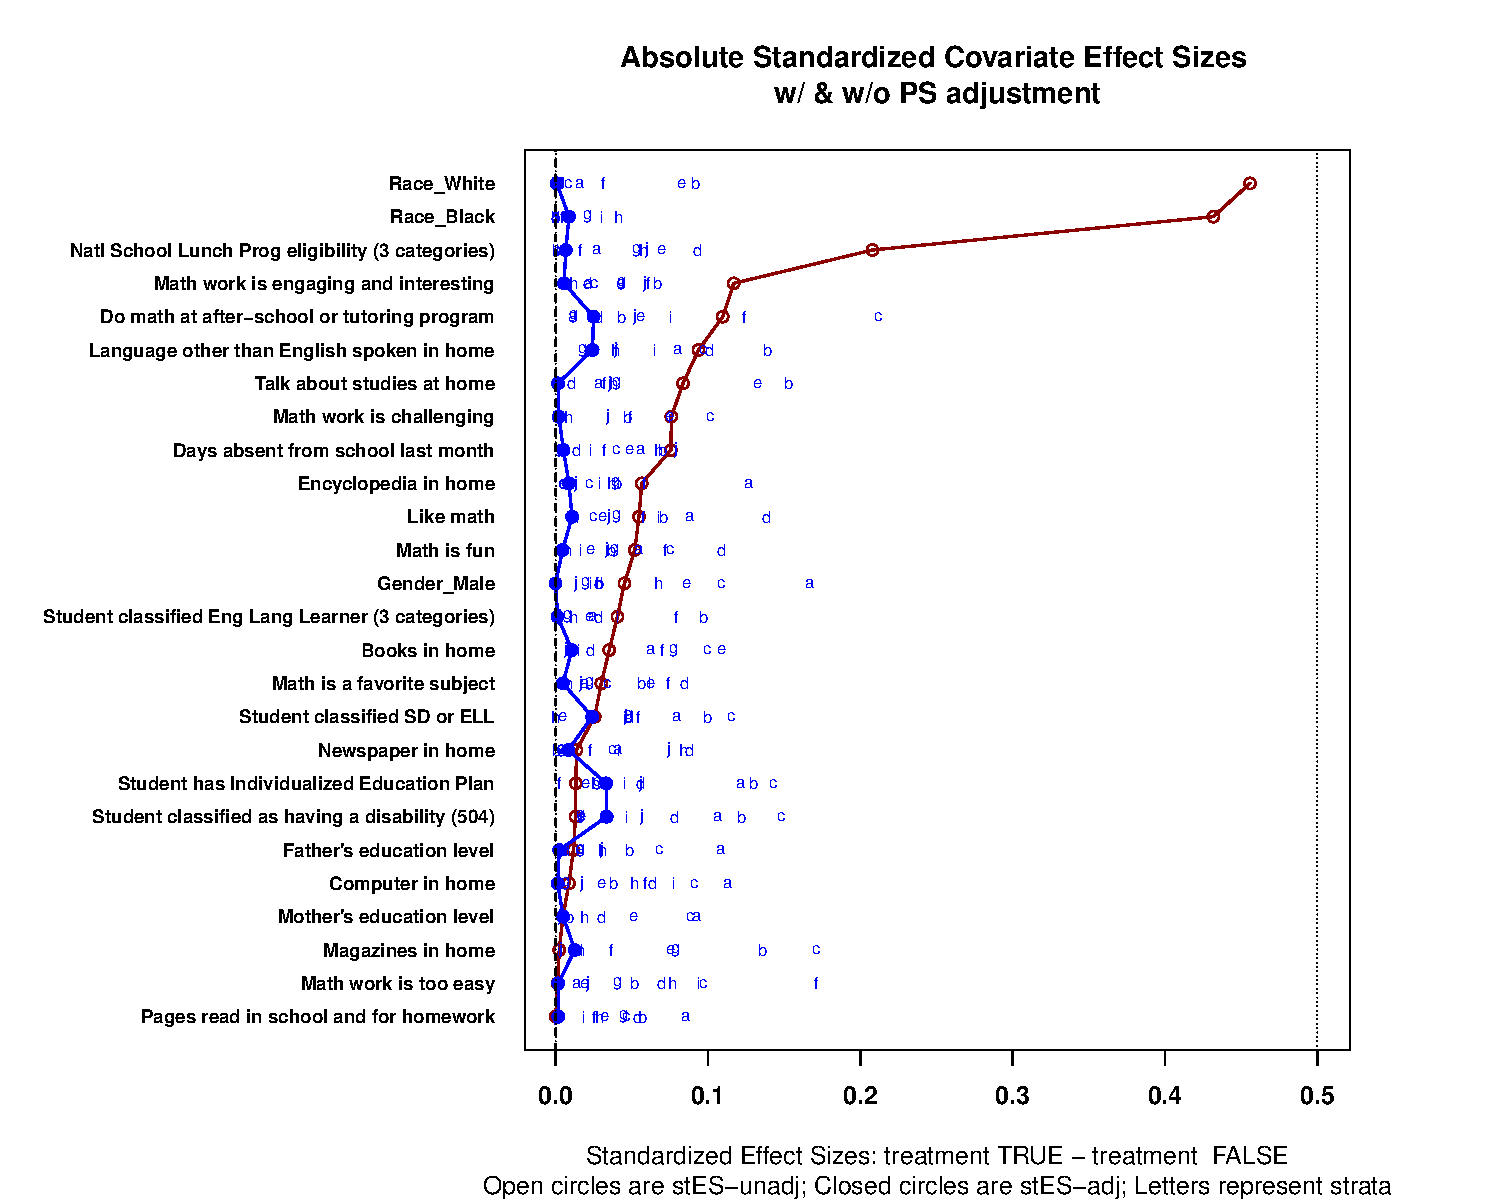
\includegraphics[width=\textwidth]{../Figures2009/g8math-lr-balance.pdf}
\caption{Covariate balance plot for logistic regression stratification: Grade 8 math}
\end{center}
\end{figure}

\begin{figure}
\begin{center}
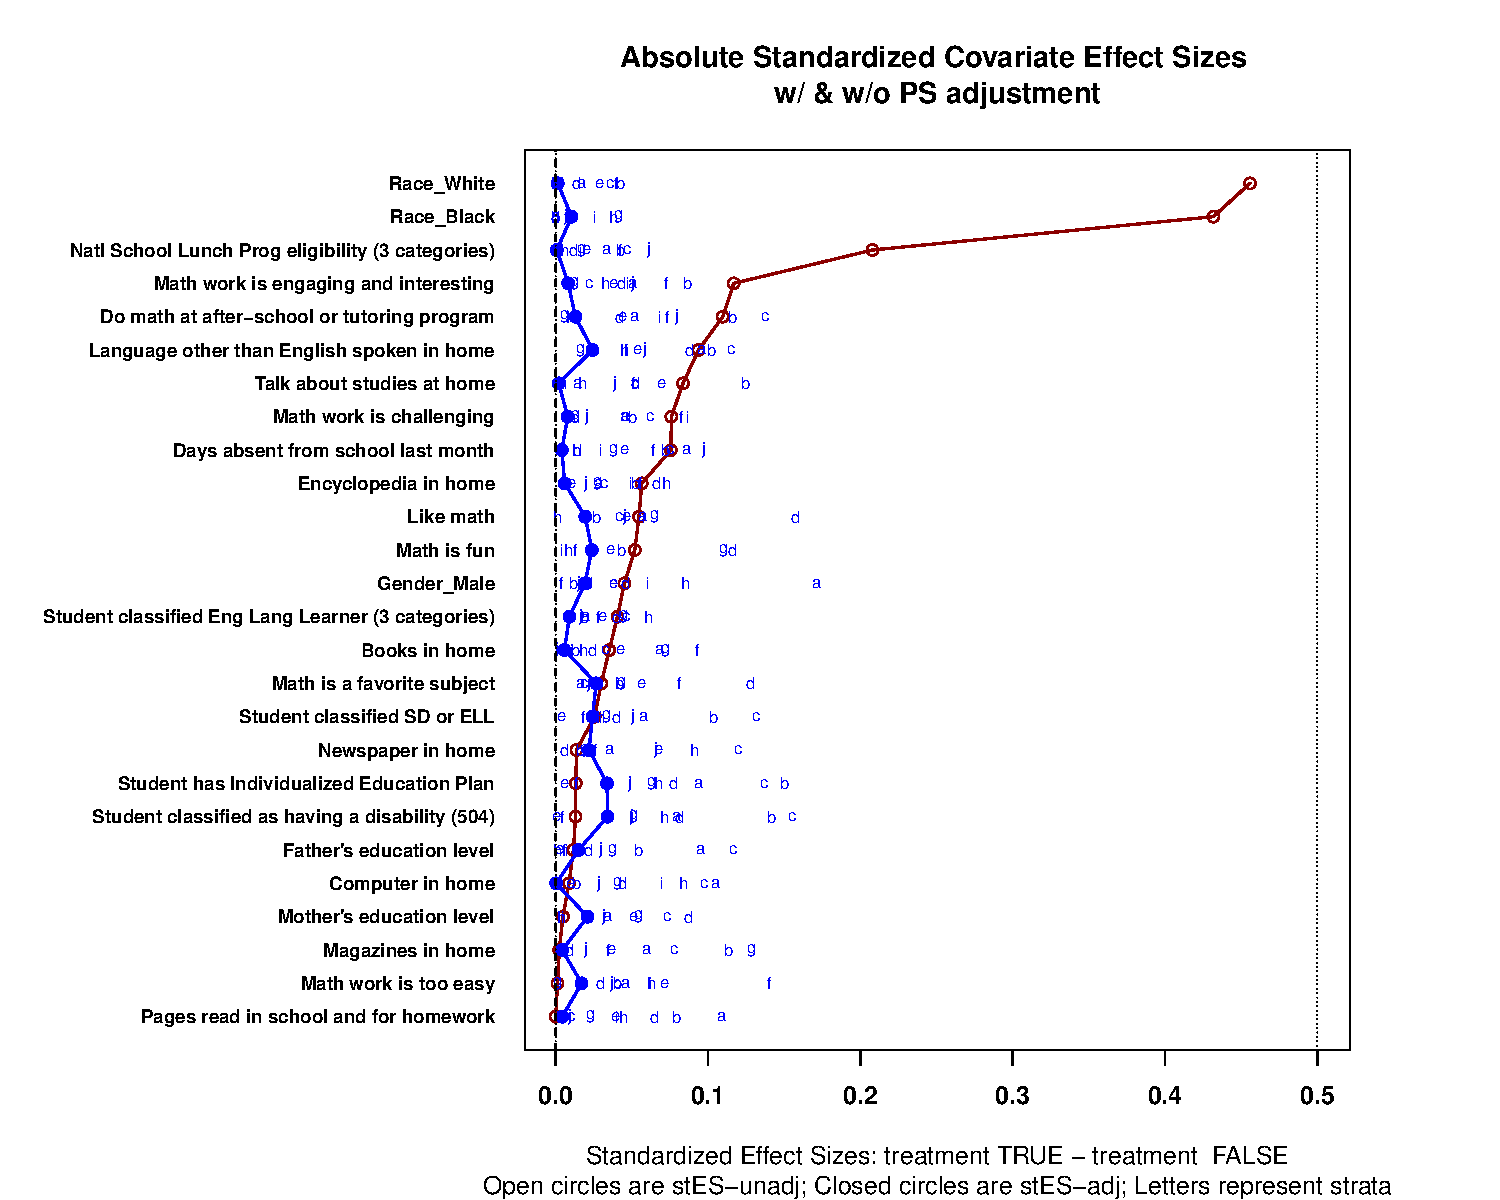
\includegraphics[width=\textwidth]{../Figures2009/g8math-lrAIC-balance.pdf}
\caption{Covariate balance plot for logistic regression AIC stratification: Grade 8 math}
\end{center}
\end{figure}

\begin{figure}
\begin{center}
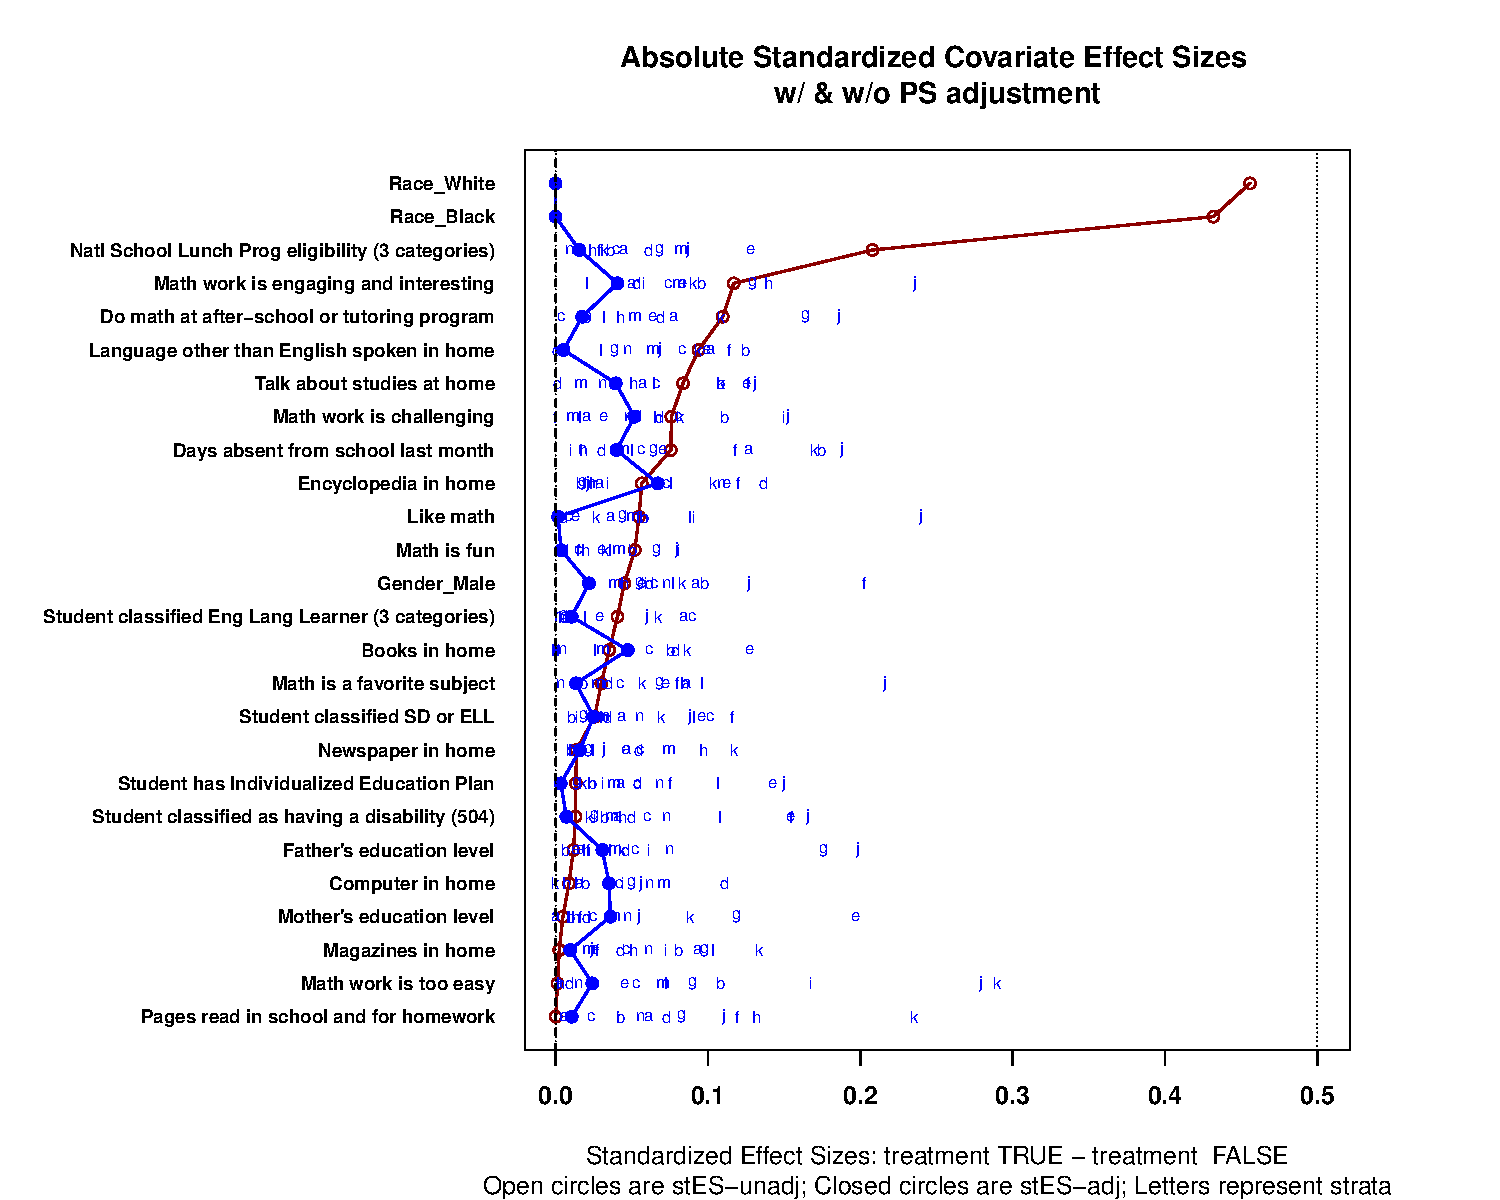
\includegraphics[width=\textwidth]{../Figures2009/g8math-tree-balance.pdf}
\caption{Covariate balance plot for classification tree stratification: Grade 8 math}
\end{center}
\end{figure}

% Grade 8 reading
\begin{figure}[h!]
\begin{center}
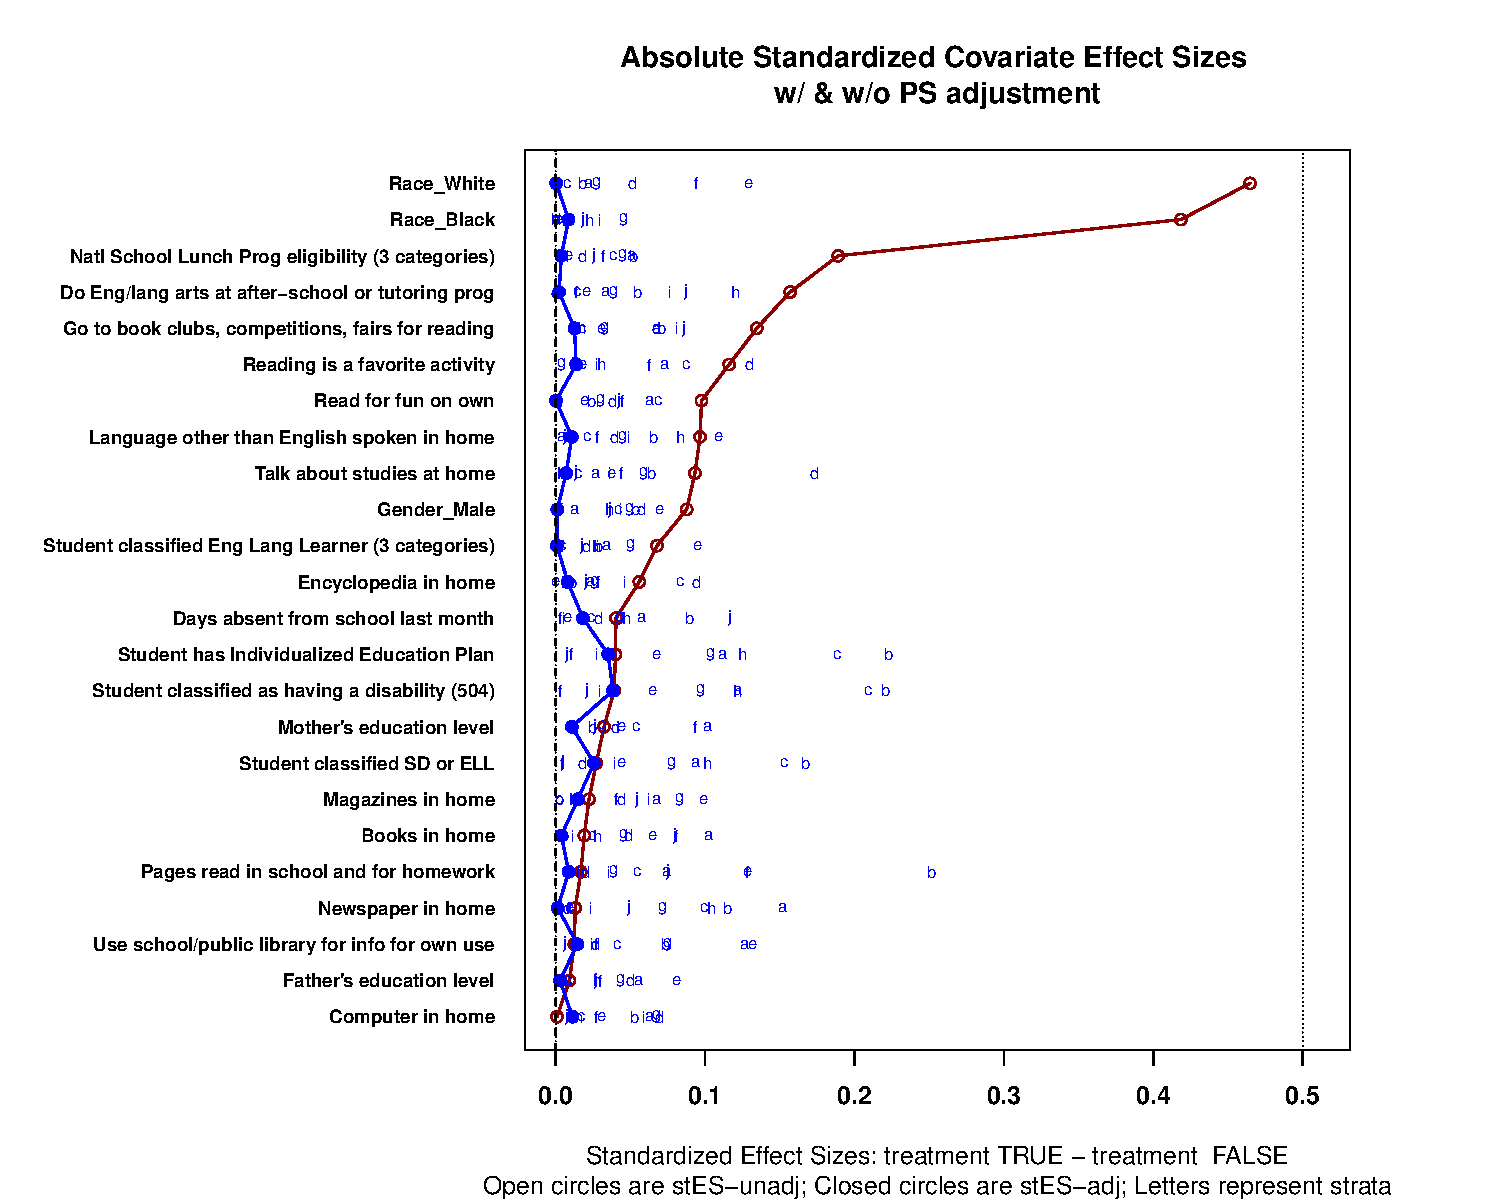
\includegraphics[width=\textwidth]{../Figures2009/g8read-lr-balance.pdf}
\caption{Covariate balance plot for logistic regression stratification: Grade 8 reading}
\end{center}
\end{figure}

\begin{figure}
\begin{center}
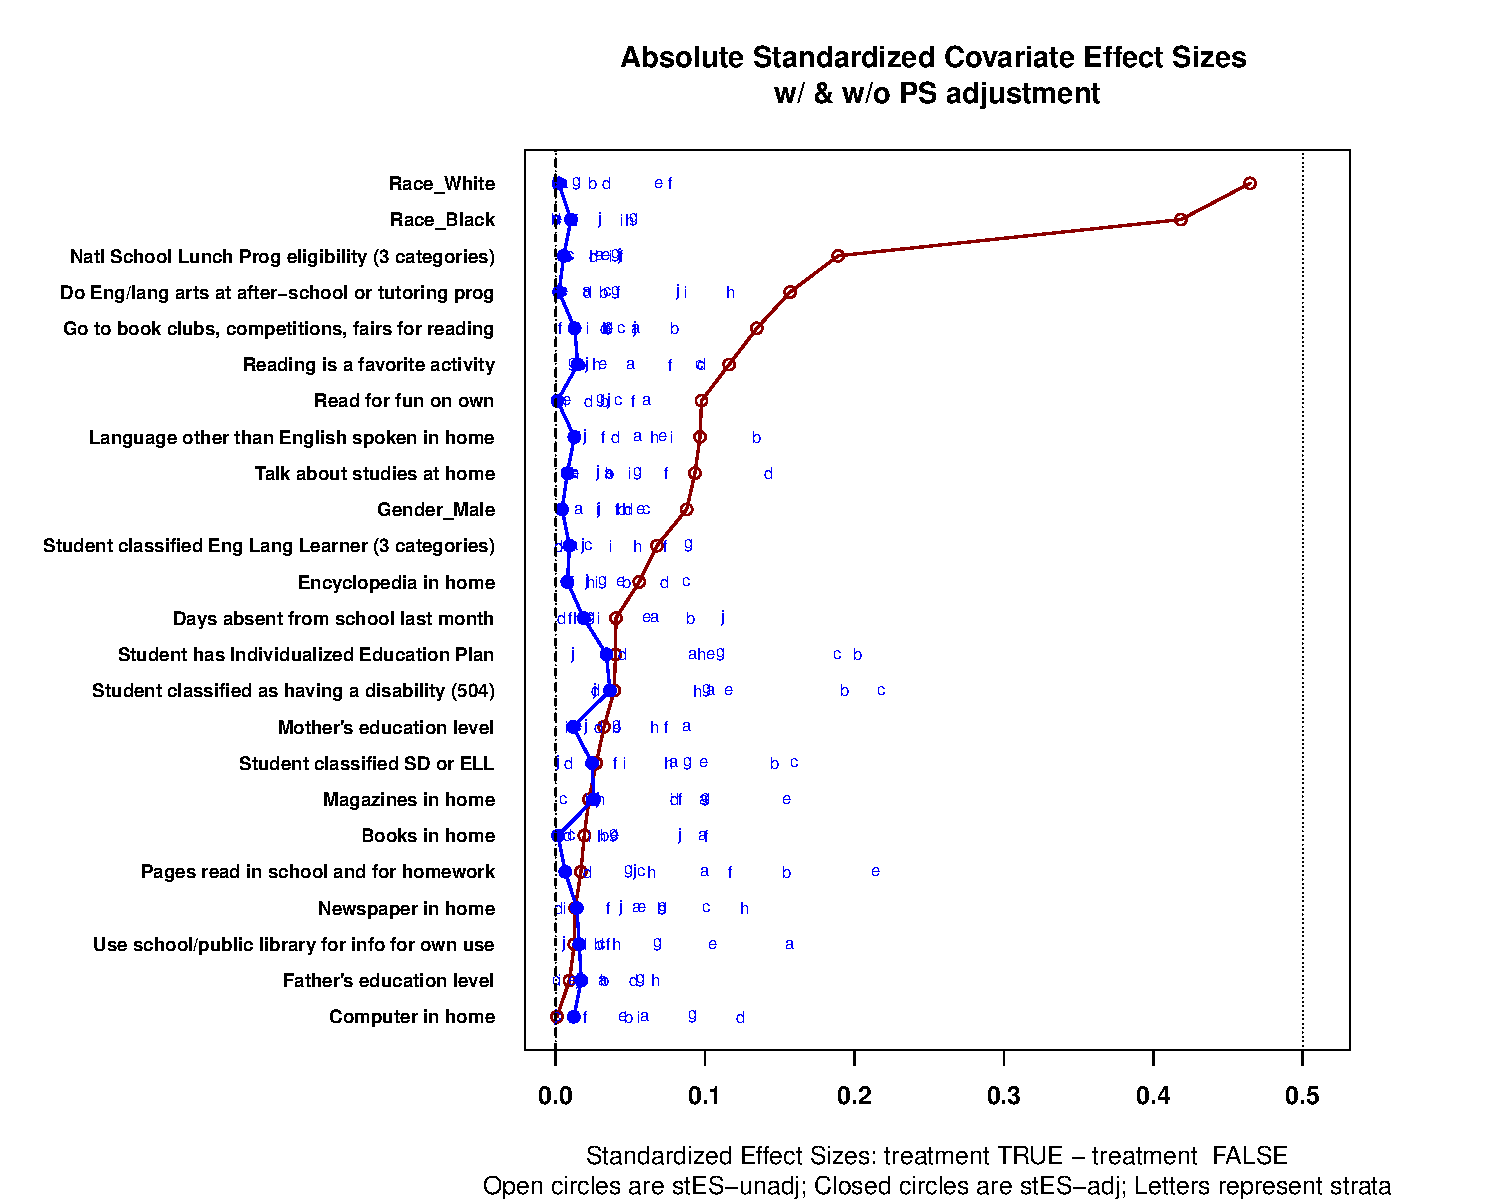
\includegraphics[width=\textwidth]{../Figures2009/g8read-lrAIC-balance.pdf}
\caption{Covariate balance plot for logistic regression AIC stratification: Grade 8 reading}
\end{center}
\end{figure}

\begin{figure}
\begin{center}
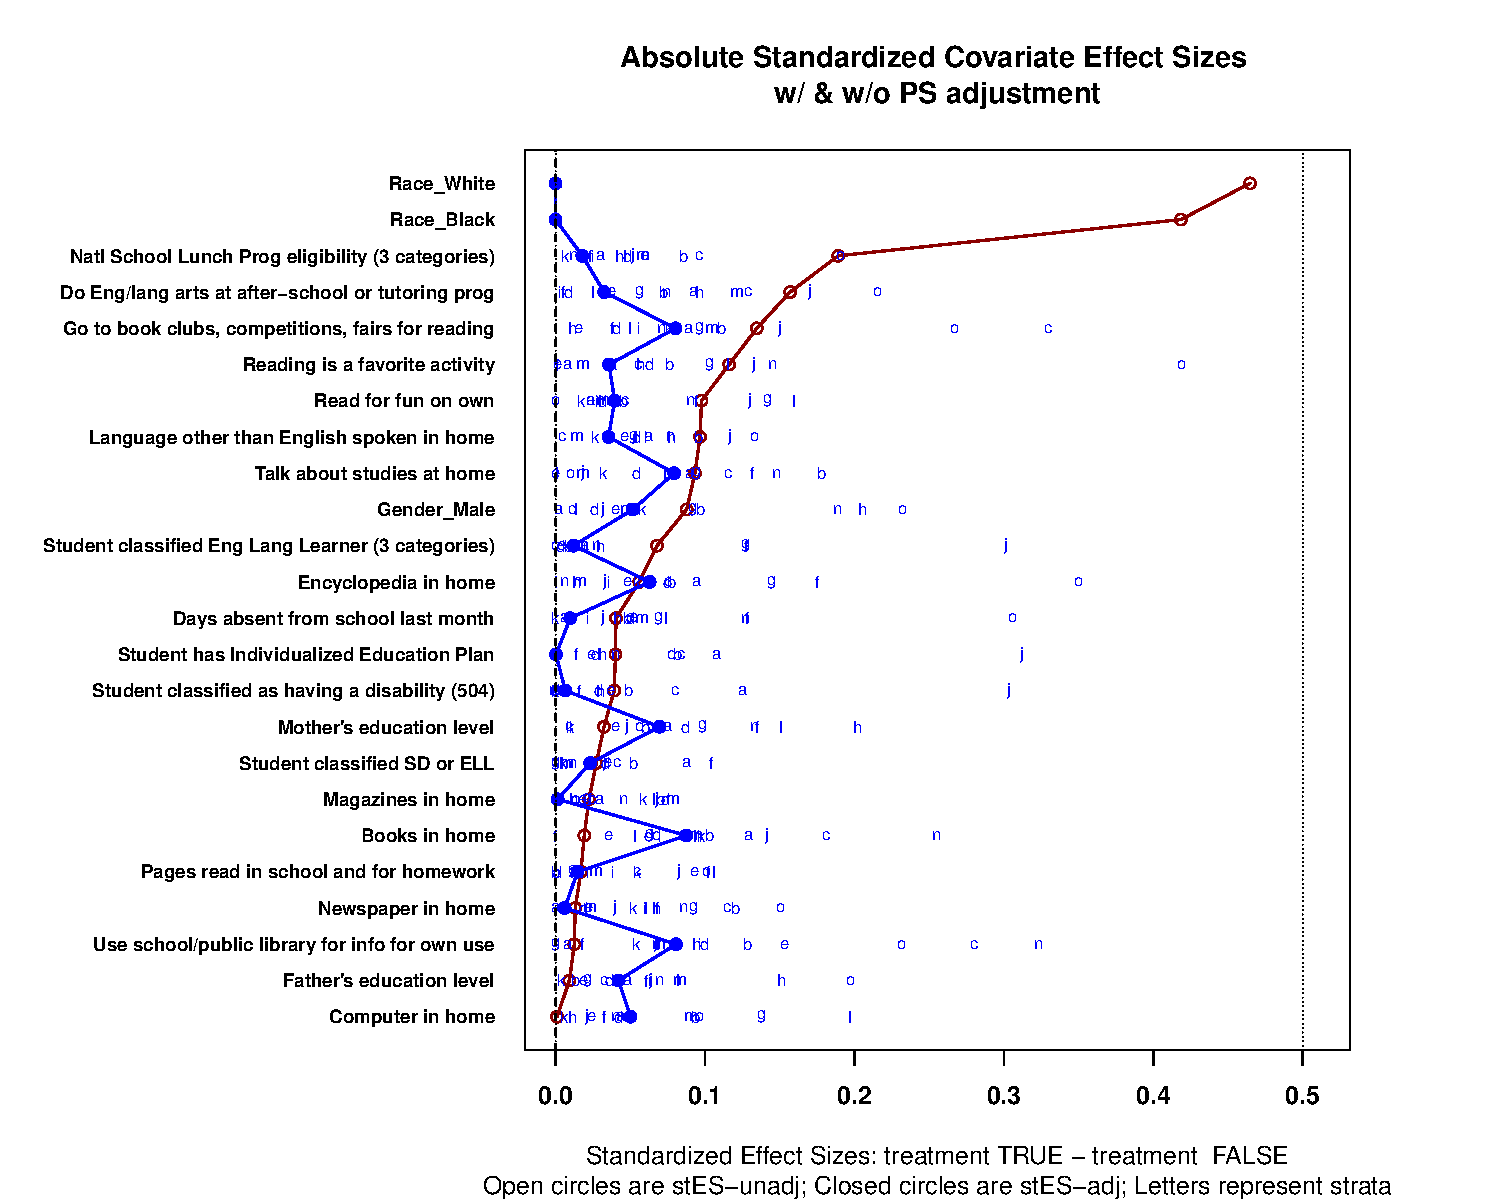
\includegraphics[width=\textwidth]{../Figures2009/g8read-tree-balance.pdf}
\caption{Covariate balance plot for classification tree stratification: Grade 8 reading}
\end{center}
\end{figure}

%==================== Appendix F ====================================================================
\clearpage
\addcontentsline{toc}{subsection}{Appendix F: Classification Method Results}
\section*{Appendix F\\Classification Method Results}
\label{appendixF}

% Grade 4 reading
\begin{figure}[h!]
\begin{center}
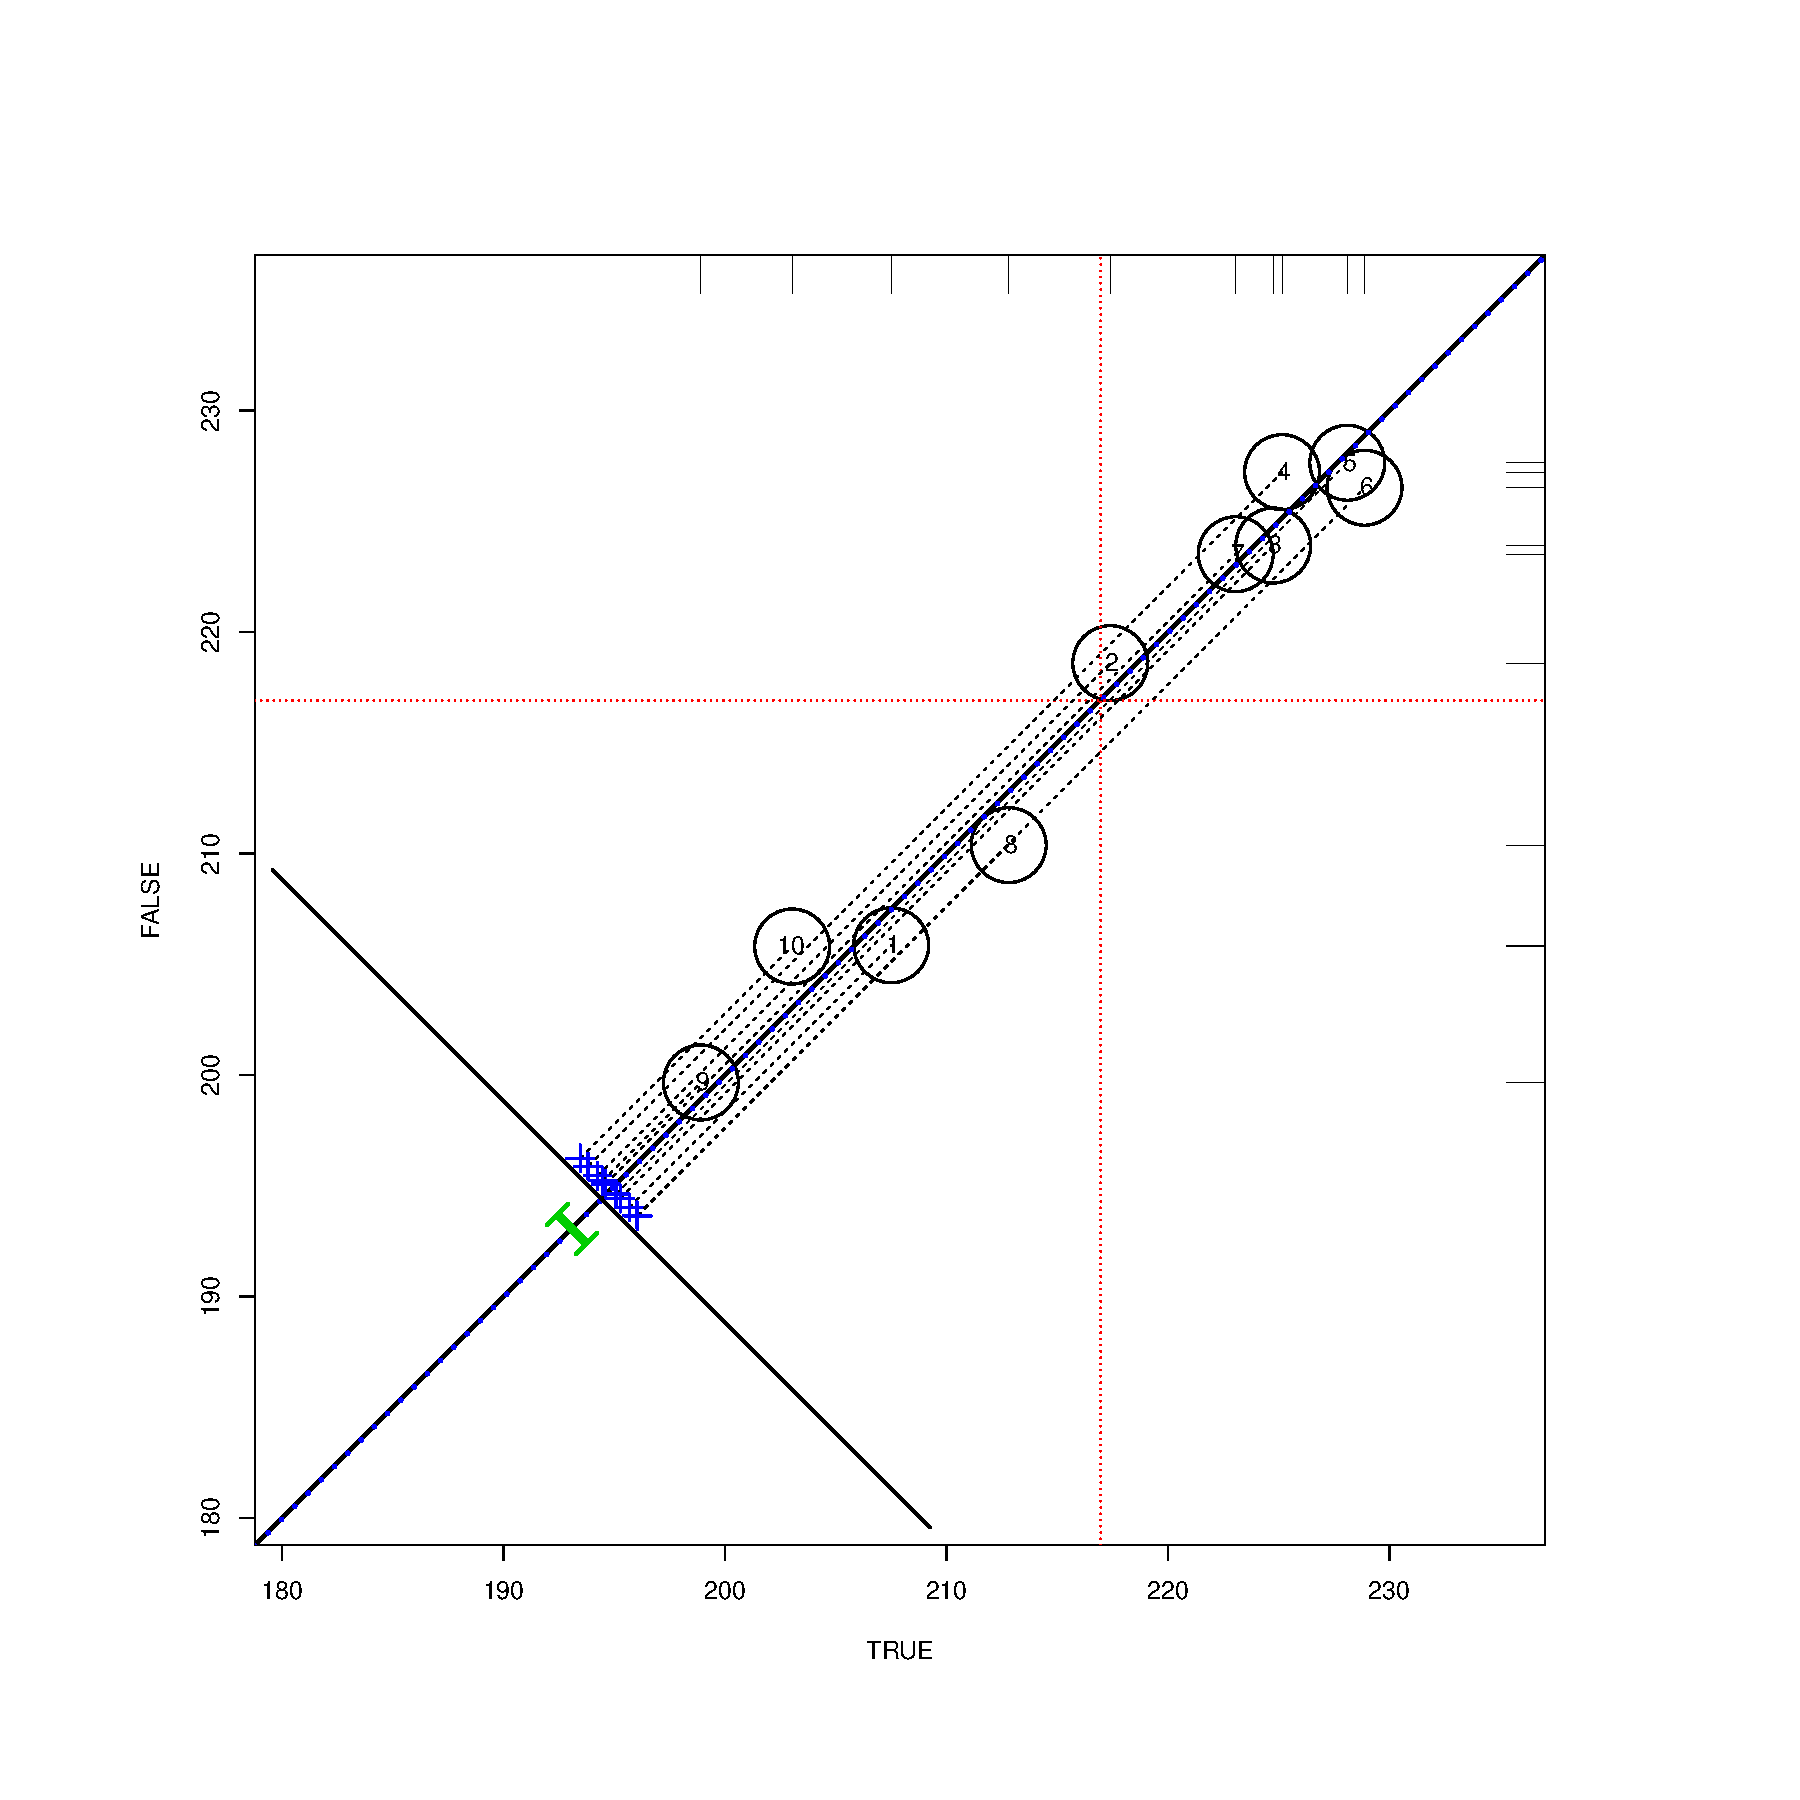
\includegraphics[height=.4\textheight,width=.4\textheight]{../Figures2009/g4read-circpsa10.pdf}
\caption{Propensity score assessment plot for logistic regression stratification: Grade 4 reading}
\end{center}
\end{figure}

% latex table generated in R 3.0.2 by xtable 1.7-1 package
% Sun Feb 23 12:17:36 2014
{\normalsize
\begin{table}[h!]
\centering
\caption{Logistic regression stratification results for grade 4 reading} 
\label{g4read-circpsa10}
\begin{tabular}{lrr@{\extracolsep{.2cm}}rr}
  \hline
   & \multicolumn{2}{c}{Public} & \multicolumn{2}{c}{Charter} \\ \cline{2-3} \cline{4-5} Strata & Mean & n & Mean & n \\ \hline
1 & 205.86 & 9440 & 207.51 & 201 \\ 
  2 & 218.60 & 9396 & 217.40 & 244 \\ 
  3 & 223.91 & 9439 & 224.76 & 202 \\ 
  4 & 227.23 & 9403 & 225.16 & 236 \\ 
  5 & 227.65 & 9371 & 228.10 & 270 \\ 
  6 & 226.52 & 9334 & 228.88 & 306 \\ 
  7 & 223.52 & 9317 & 223.07 & 323 \\ 
  8 & 210.39 & 9292 & 212.81 & 348 \\ 
  9 & 199.67 & 8990 & 198.92 & 650 \\ 
  10 & 205.81 & 8774 & 203.04 & 867 \\ 
   \hline
\end{tabular}
\end{table}
}


\clearpage

\begin{figure}
\begin{center}
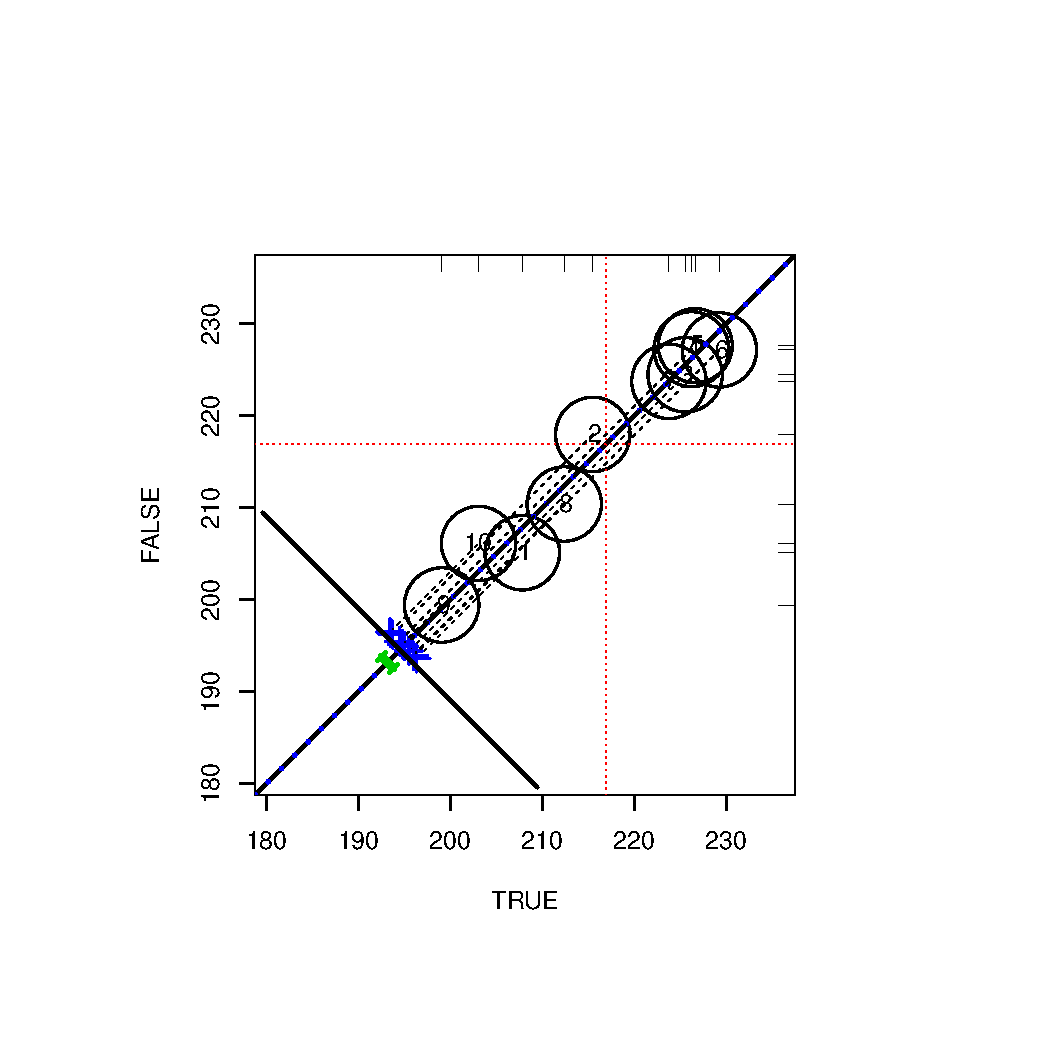
\includegraphics[height=.4\textheight,width=.4\textheight]{../Figures2009/g4read-circpsa10-AIC.pdf}
\caption{Propensity score assessment plot for logistic regression AIC stratification: Grade 4 reading}
\end{center}
\end{figure}

% latex table generated in R 3.0.2 by xtable 1.7-1 package
% Sun Feb 23 12:17:36 2014
\begin{table}[h!]
\centering
\caption{Logistic regression AIC stratification results for grade 4 reading} 
\label{g4read-circpsa10AIC}
\begin{tabular}{lrr@{\extracolsep{.2cm}}rr}
  \hline
   & \multicolumn{2}{c}{Public} & \multicolumn{2}{c}{Charter} \\ \cline{2-3} \cline{4-5} Strata & Mean & n & Mean & n \\ \hline
1 & 205.11 & 9434 & 207.83 & 218 \\ 
  2 & 217.96 & 9415 & 215.48 & 215 \\ 
  3 & 224.45 & 9406 & 225.53 & 233 \\ 
  4 & 227.24 & 9562 & 226.22 & 230 \\ 
  5 & 227.62 & 9241 & 226.63 & 263 \\ 
  6 & 227.15 & 9341 & 229.26 & 284 \\ 
  7 & 223.73 & 9296 & 223.77 & 354 \\ 
  8 & 210.40 & 9293 & 212.38 & 337 \\ 
  9 & 199.42 & 8996 & 199.06 & 648 \\ 
  10 & 206.10 & 8772 & 203.07 & 865 \\ 
   \hline
\end{tabular}
\end{table}


\clearpage

\begin{figure}
\begin{center}
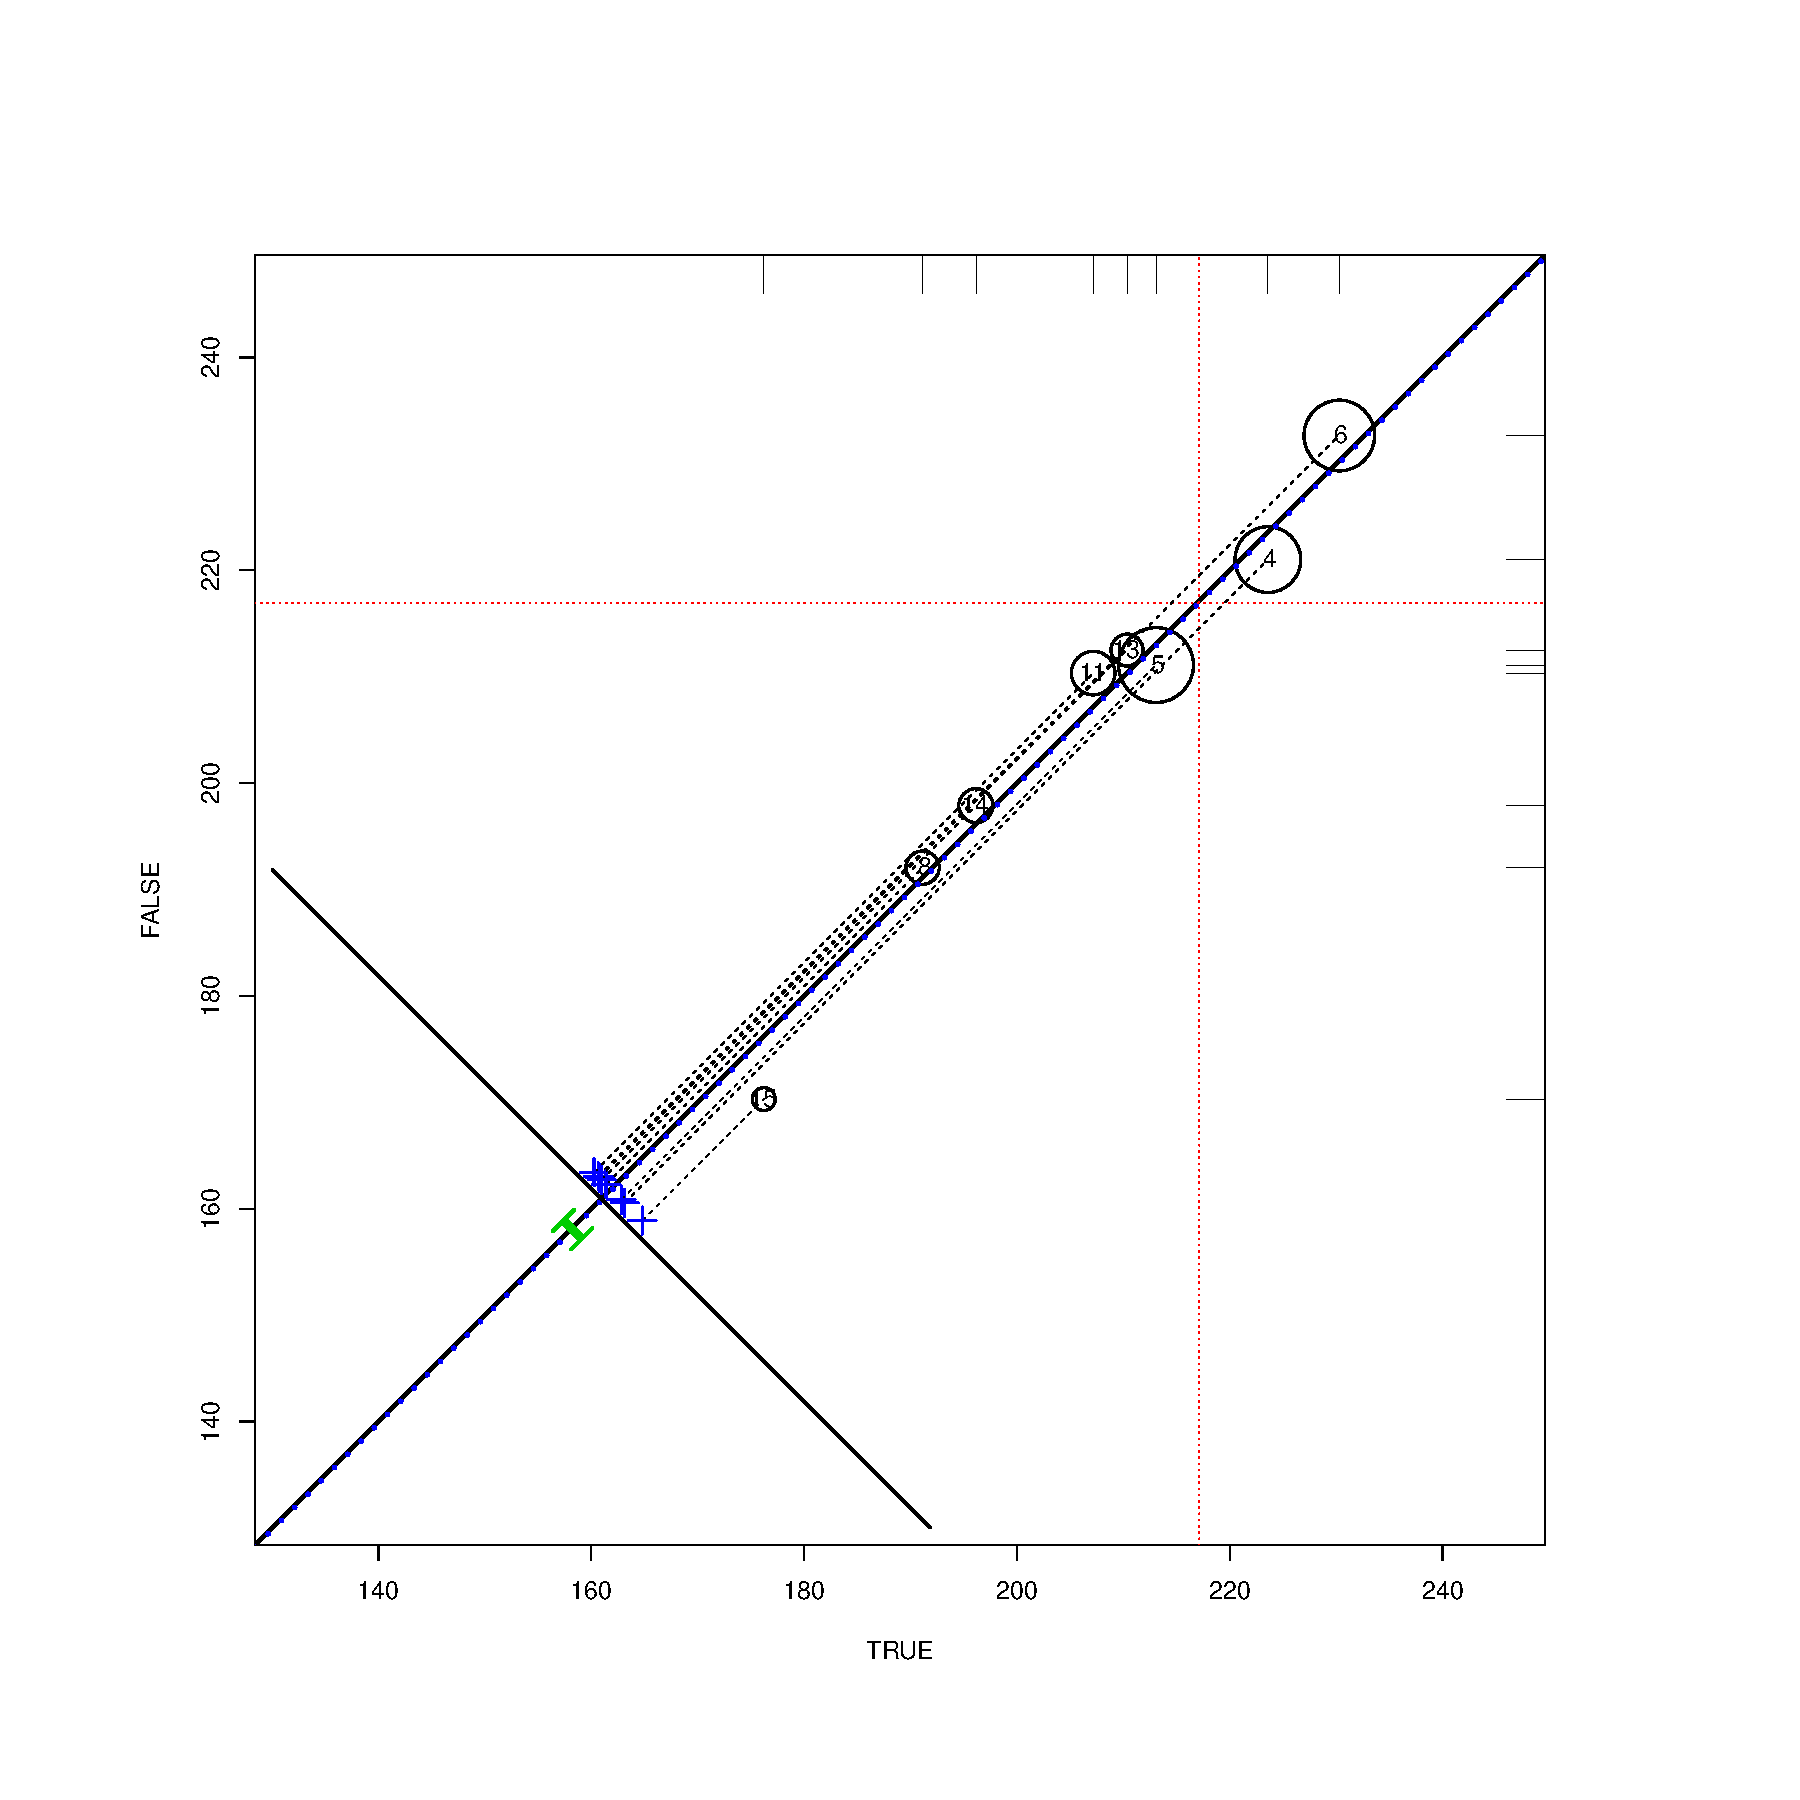
\includegraphics[height=.4\textheight,width=.4\textheight]{../Figures2009/g4read-circpsa-tree.pdf}
\caption{Propensity score assessment plot for classification tree stratification: Grade 4 reading}
\end{center}
\end{figure}

% latex table generated in R 3.0.2 by xtable 1.7-1 package
% Sun Feb 23 12:17:36 2014
\begin{table}[ht]
\centering
\caption{Classification Trees Stratification Results for Grade 4 read} 
\label{g4read-circpsa-tree}
\begin{tabular}{lrr@{\extracolsep{.2cm}}rr}
  \hline
   & \multicolumn{2}{c}{Public} & \multicolumn{2}{c}{Charter} \\ \cline{2-3} \cline{4-5} Strata & Mean & n & Mean & n \\ \hline
4 & 220.99 & 20677 & 223.57 & 464 \\ 
  5 & 211.08 & 28477 & 213.06 & 826 \\ 
  6 & 232.65 & 24503 & 230.28 & 785 \\ 
  8 & 192.06 & 3690 & 191.14 & 223 \\ 
  11 & 210.33 & 7001 & 207.16 & 547 \\ 
  13 & 212.50 & 3225 & 210.35 & 294 \\ 
  14 & 197.88 & 3735 & 196.15 & 429 \\ 
  15 & 170.31 & 1448 & 176.22 &  79 \\ 
   \hline
\end{tabular}
\end{table}


% Grade 8 math
\begin{figure}[h!]
\begin{center}
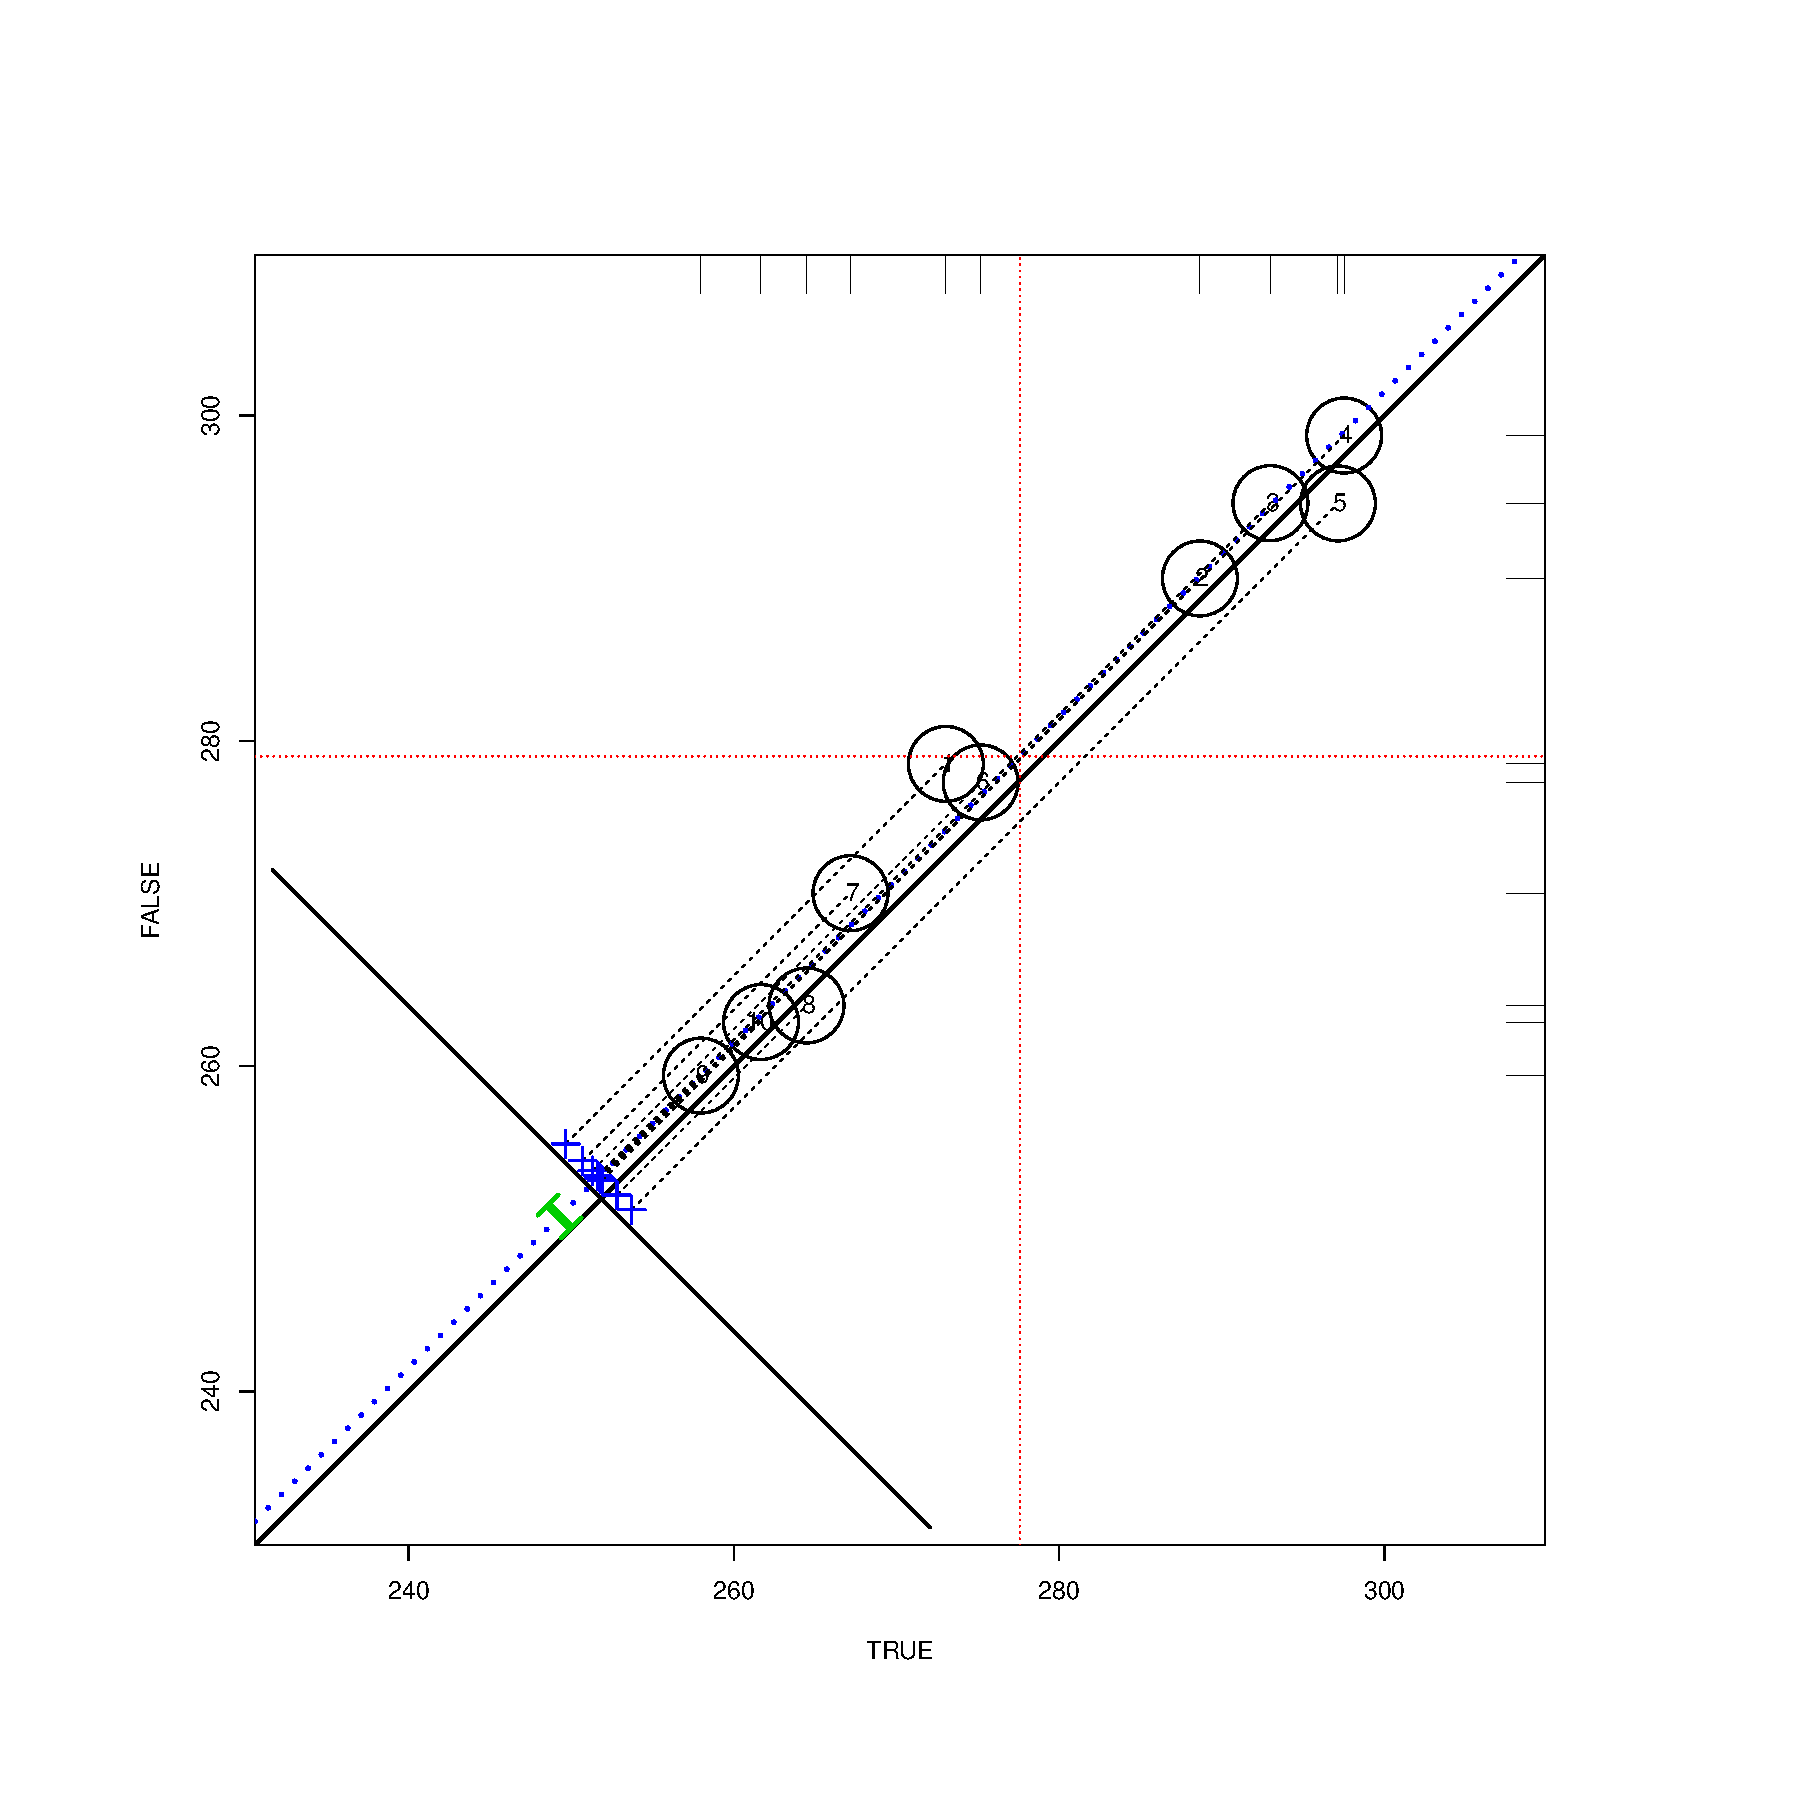
\includegraphics[height=.4\textheight,width=.4\textheight]{../Figures2009/g8math-circpsa10.pdf}
\caption{Propensity score assessment plot for logistic regression stratification: Grade 8 math}
\end{center}
\end{figure}

% latex table generated in R 3.0.1 by xtable 1.7-1 package
% Thu Jun 20 13:40:46 2013
\begin{table}[ht]
\centering
\caption{Logistic Regression Stratification Results for Grade 8 math} 
\label{g8math-circpsa10}
\begin{tabular}{lrr@{\extracolsep{.2cm}}rr}
  \hline
   & \multicolumn{2}{c}{Public} & \multicolumn{2}{c}{Charter} \\ \cline{2-3} \cline{4-5} Strata & Mean & n & Mean & n \\ \hline
1 & 278.58 & 7402 & 273.03 & 135 \\ 
  2 & 289.98 & 7359 & 288.65 & 177 \\ 
  3 & 294.62 & 7334 & 292.99 & 202 \\ 
  4 & 298.77 & 7292 & 297.52 & 244 \\ 
  5 & 294.60 & 7207 & 297.14 & 329 \\ 
  6 & 277.44 & 7183 & 275.17 & 353 \\ 
  7 & 270.63 & 7132 & 267.17 & 404 \\ 
  8 & 263.73 & 7022 & 264.47 & 514 \\ 
  9 & 259.42 & 6864 & 257.97 & 672 \\ 
  10 & 262.71 & 6733 & 261.67 & 803 \\ 
   \hline
\end{tabular}
\end{table}


\clearpage
\begin{figure}
\begin{center}
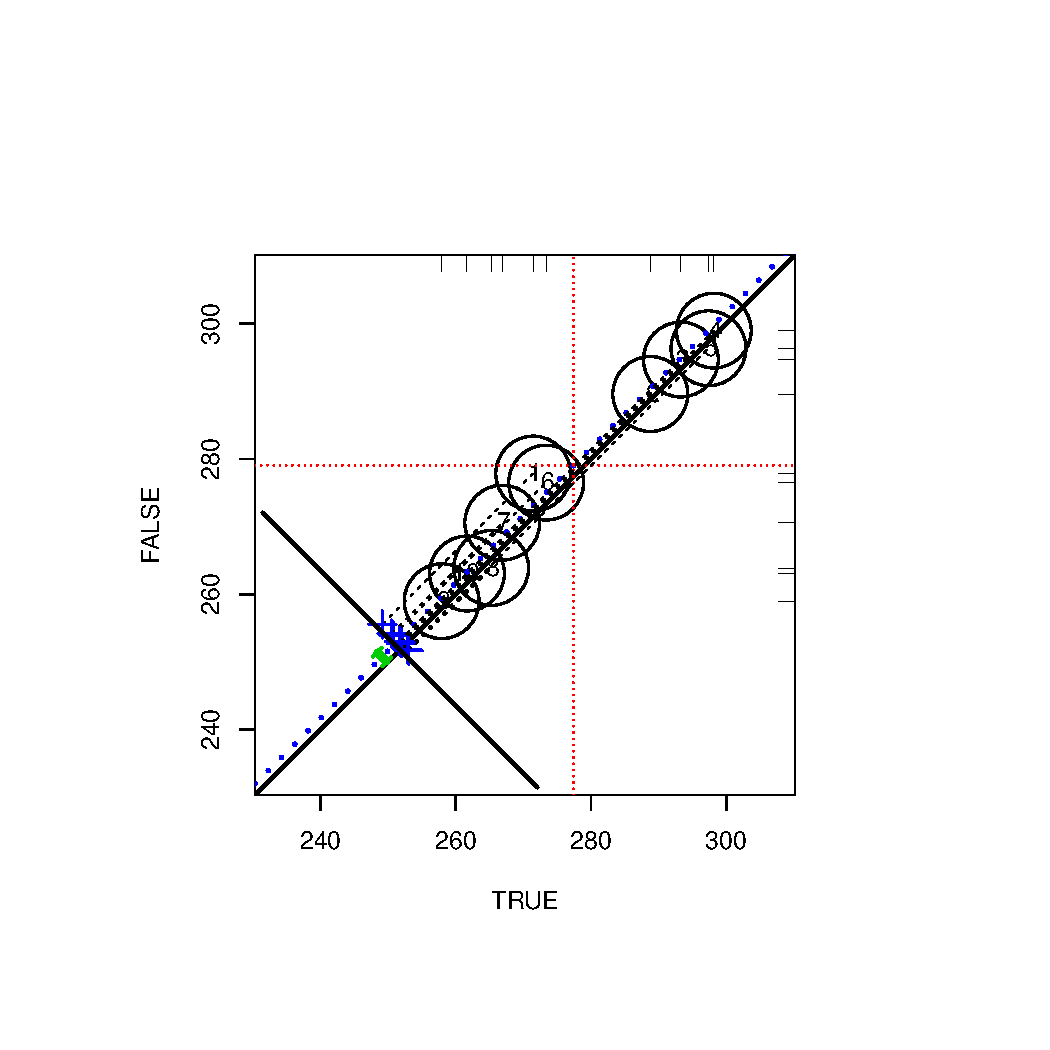
\includegraphics[height=.4\textheight,width=.4\textheight]{../Figures2009/g8math-circpsa10-AIC.pdf}
\caption{Propensity score assessment plot for logistic regression AIC stratification: Grade 8 math}
\end{center}
\end{figure}

% latex table generated in R 3.0.2 by xtable 1.7-1 package
% Sun Feb 23 12:19:00 2014
\begin{table}[ht]
\centering
\caption{Logistic regression AIC stratification results for grade 8 math} 
\label{g8math-circpsa10AIC}
\begin{tabular}{lrr@{\extracolsep{.2cm}}rr}
  \hline
   & \multicolumn{2}{c}{Public} & \multicolumn{2}{c}{Charter} \\ \cline{2-3} \cline{4-5} Strata & Mean & n & Mean & n \\ \hline
1 & 277.84 & 7407 & 271.47 & 135 \\ 
  2 & 289.62 & 7388 & 288.77 & 172 \\ 
  3 & 294.71 & 7324 & 293.29 & 211 \\ 
  4 & 299.00 & 7268 & 298.16 & 240 \\ 
  5 & 296.38 & 7199 & 297.38 & 338 \\ 
  6 & 276.51 & 7193 & 273.37 & 342 \\ 
  7 & 270.59 & 7122 & 266.88 & 417 \\ 
  8 & 263.89 & 7033 & 265.24 & 512 \\ 
  9 & 258.98 & 6862 & 257.92 & 666 \\ 
  10 & 263.08 & 6732 & 261.66 & 800 \\ 
   \hline
\end{tabular}
\end{table}


\clearpage
\begin{figure}
\begin{center}
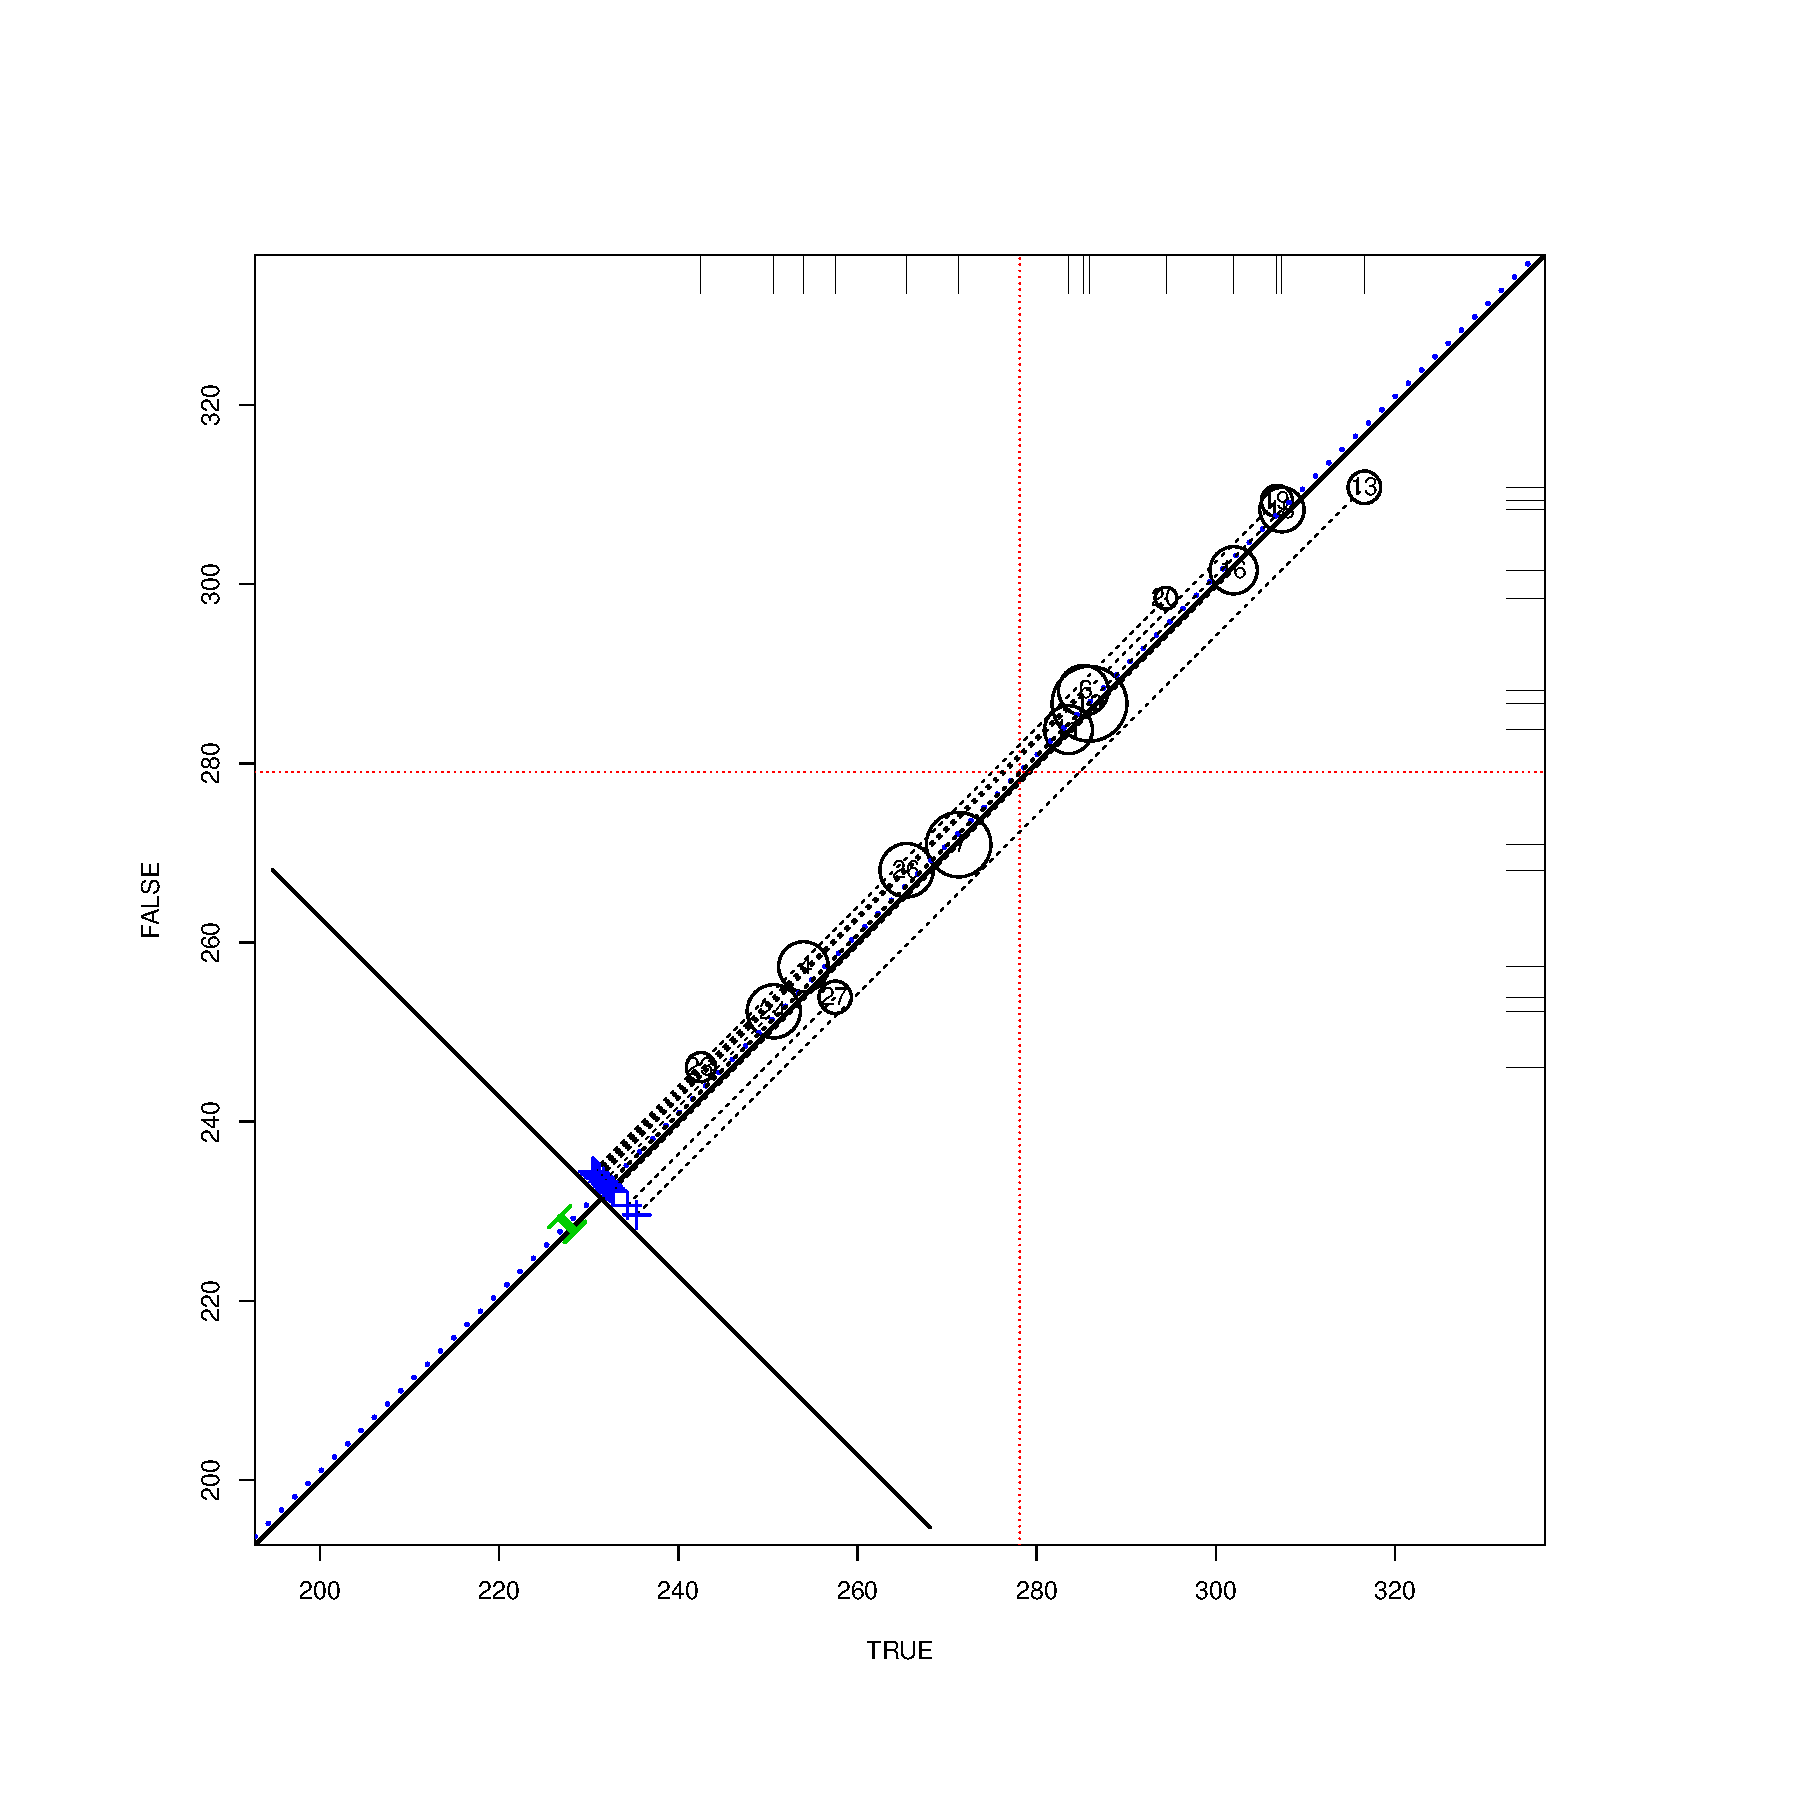
\includegraphics[height=.4\textheight,width=.4\textheight]{../Figures2009/g8math-circpsa-tree.pdf}
\caption{Propensity score assessment plot for classification tree stratification: Grade 8 math}
\end{center}
\end{figure}

% latex table generated in R 3.0.2 by xtable 1.7-1 package
% Sun Feb 23 12:19:00 2014
\begin{table}[ht]
\centering
\caption{Classification Trees Stratification Results for Grade 8 math} 
\label{g8math-circpsa-tree}
\begin{tabular}{lrr@{\extracolsep{.2cm}}rr}
  \hline
   & \multicolumn{2}{c}{Public} & \multicolumn{2}{c}{Charter} \\ \cline{2-3} \cline{4-5} Strata & Mean & n & Mean & n \\ \hline
4 & 257.31 & 5529 & 253.98 & 261 \\ 
  6 & 288.14 & 5544 & 285.21 & 257 \\ 
  7 & 270.93 & 10414 & 271.28 & 704 \\ 
  10 & 286.65 & 15771 & 285.89 & 318 \\ 
  11 & 283.75 & 5109 & 283.55 & 156 \\ 
  13 & 310.81 & 2000 & 316.58 &  51 \\ 
  16 & 301.54 & 4895 & 301.98 & 166 \\ 
  18 & 308.30 & 4163 & 307.37 & 172 \\ 
  19 & 309.29 & 1720 & 306.81 & 106 \\ 
  20 & 298.44 & 694 & 294.44 &  48 \\ 
  23 & 246.10 & 1432 & 242.53 &  92 \\ 
  24 & 252.32 & 6261 & 250.66 & 581 \\ 
  26 & 268.06 & 6244 & 265.49 & 670 \\ 
  27 & 253.90 & 1752 & 257.52 & 251 \\ 
   \hline
\end{tabular}
\end{table}


% Grade 8 reading
\clearpage
\begin{figure}[h!]
\begin{center}
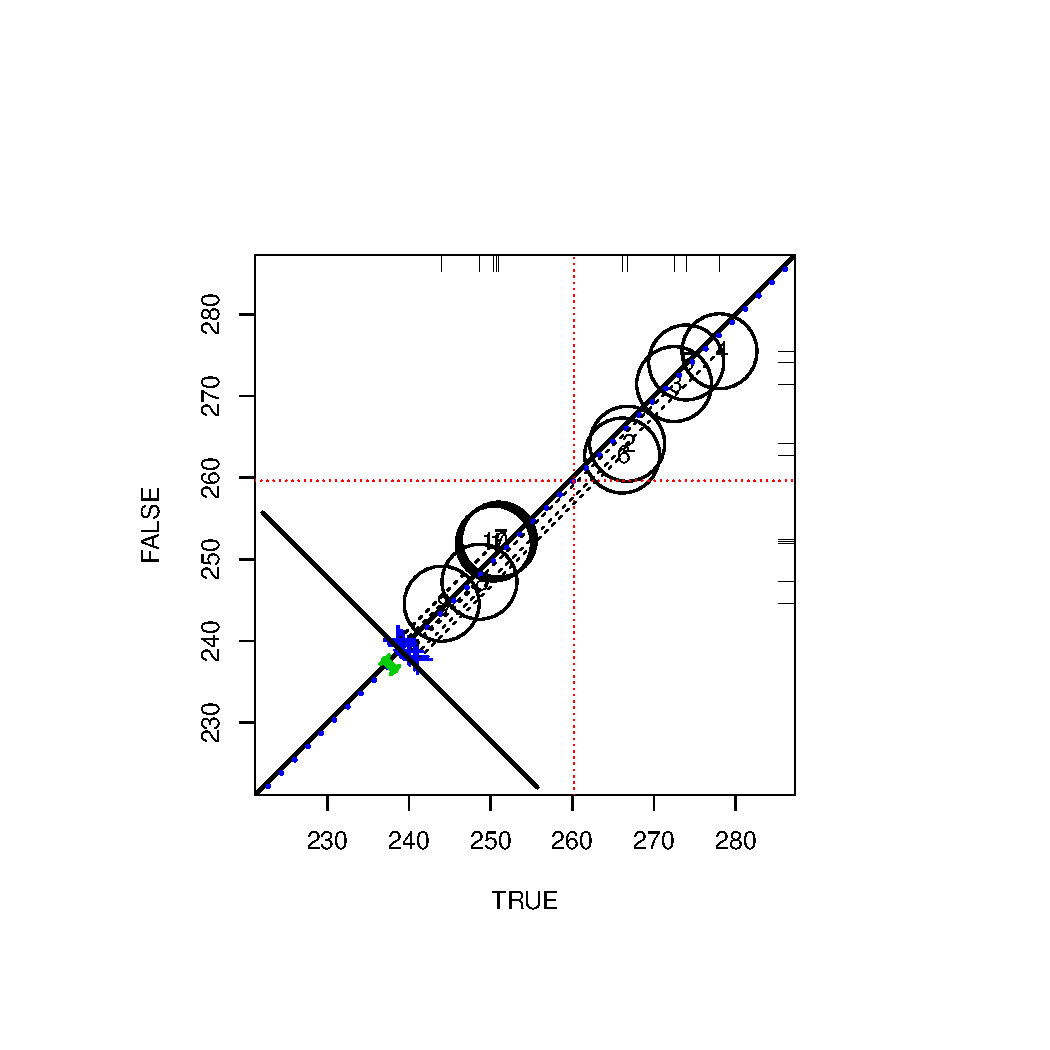
\includegraphics[height=.4\textheight,width=.4\textheight]{../Figures2009/g8read-circpsa10.pdf}
\caption{Propensity score assessment plot for logistic regression stratification: Grade 8 reading}
\end{center}
\end{figure}

% latex table generated in R 3.0.2 by xtable 1.7-1 package
% Sun Feb 23 12:20:17 2014
\begin{table}[h!]
\centering
\caption{Logistic regression stratification results for grade 8 reading} 
\label{g8read-circpsa10}
\begin{tabular}{lrr@{\extracolsep{.2cm}}rr}
  \hline
   & \multicolumn{2}{c}{Public} & \multicolumn{2}{c}{Charter} \\ \cline{2-3} \cline{4-5} Strata & Mean & n & Mean & n \\ \hline
1 & 251.94 & 7634 & 250.40 & 129 \\ 
  2 & 264.16 & 7596 & 266.72 & 167 \\ 
  3 & 271.47 & 7535 & 272.48 & 226 \\ 
  4 & 275.49 & 7519 & 278.03 & 243 \\ 
  5 & 274.12 & 7471 & 273.95 & 291 \\ 
  6 & 262.72 & 7413 & 266.11 & 349 \\ 
  7 & 252.41 & 7379 & 251.00 & 383 \\ 
  8 & 247.25 & 7213 & 248.63 & 549 \\ 
  9 & 244.57 & 7103 & 243.99 & 659 \\ 
  10 & 252.15 & 6947 & 250.66 & 816 \\ 
   \hline
\end{tabular}
\end{table}


\clearpage
\begin{figure}
\begin{center}
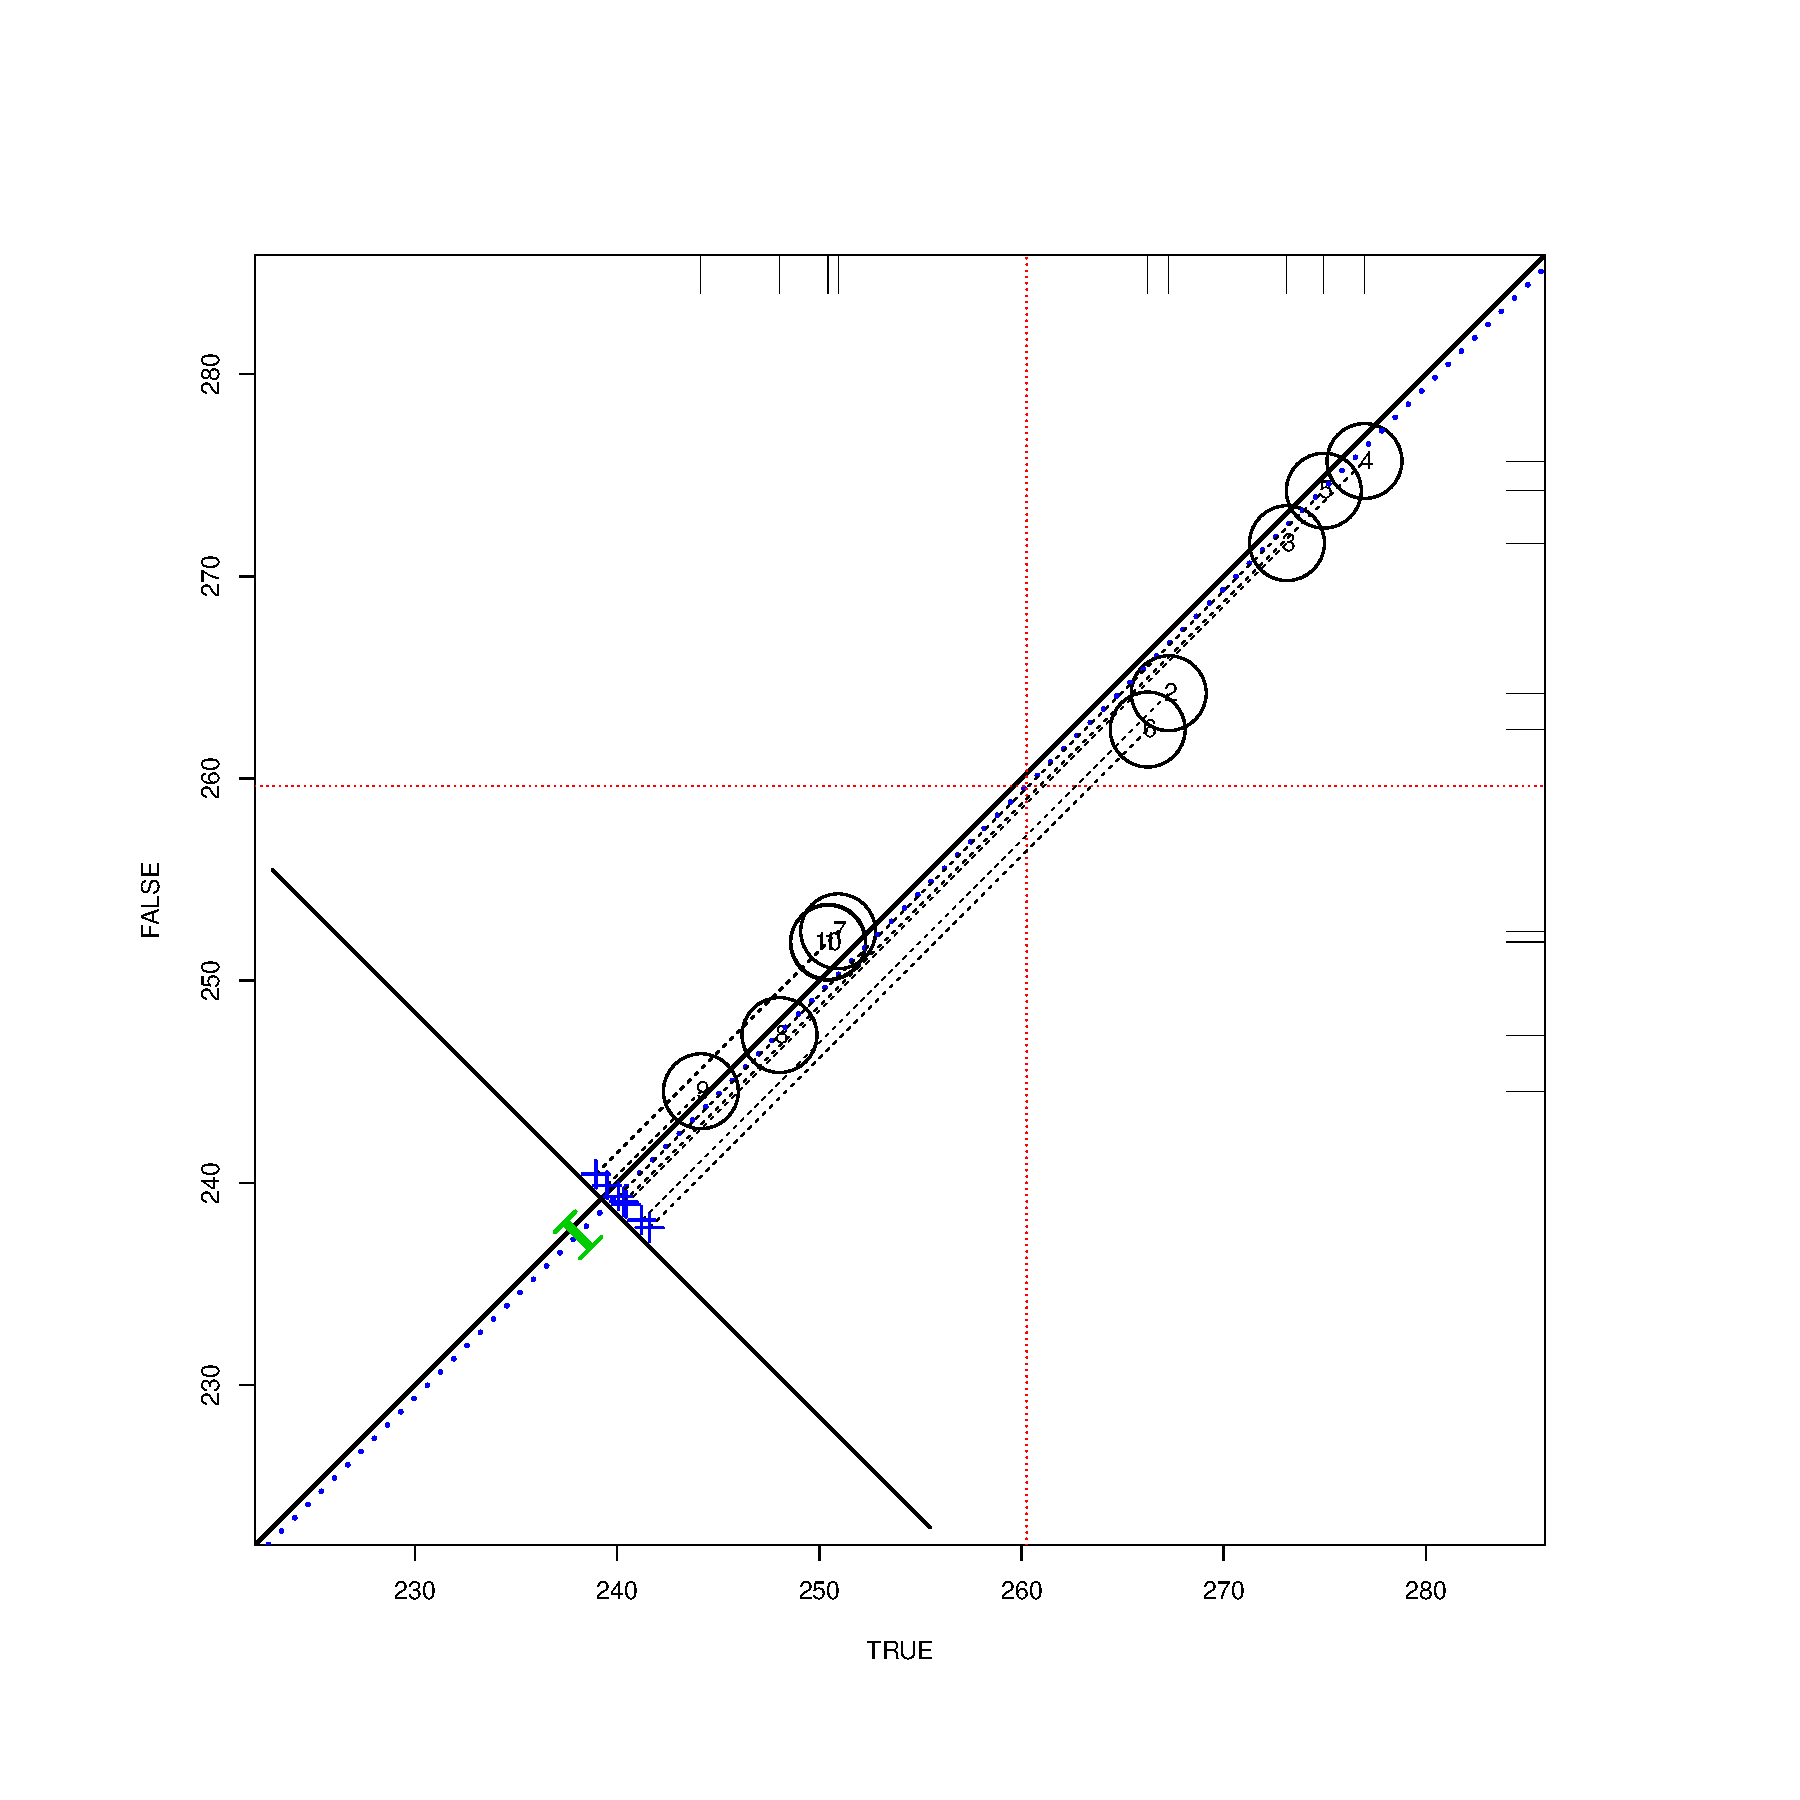
\includegraphics[height=.4\textheight,width=.4\textheight]{../Figures2009/g8read-circpsa10-AIC.pdf}
\caption{Propensity score assessment plot for logistic regression AIC stratification: Grade 8 reading}
\end{center}
\end{figure}

% latex table generated in R 3.0.2 by xtable 1.7-1 package
% Sun Feb 23 12:20:17 2014
\begin{table}[ht]
\centering
\caption{Logistic Regression AIC Stratification Results for Grade 8 read} 
\label{g8read-circpsa10AIC}
\begin{tabular}{lrr@{\extracolsep{.2cm}}rr}
  \hline
   & \multicolumn{2}{c}{Public} & \multicolumn{2}{c}{Charter} \\ \cline{2-3} \cline{4-5} Strata & Mean & n & Mean & n \\ \hline
1 & 251.87 & 7636 & 250.42 & 128 \\ 
  2 & 264.22 & 7592 & 267.28 & 169 \\ 
  3 & 271.64 & 7530 & 273.13 & 232 \\ 
  4 & 275.70 & 7530 & 276.96 & 232 \\ 
  5 & 274.23 & 7466 & 274.95 & 296 \\ 
  6 & 262.42 & 7417 & 266.24 & 345 \\ 
  7 & 252.44 & 7365 & 250.93 & 397 \\ 
  8 & 247.31 & 7208 & 248.03 & 554 \\ 
  9 & 244.53 & 7132 & 244.14 & 630 \\ 
  10 & 251.91 & 6934 & 250.44 & 829 \\ 
   \hline
\end{tabular}
\end{table}


\clearpage
\begin{figure}
\begin{center}
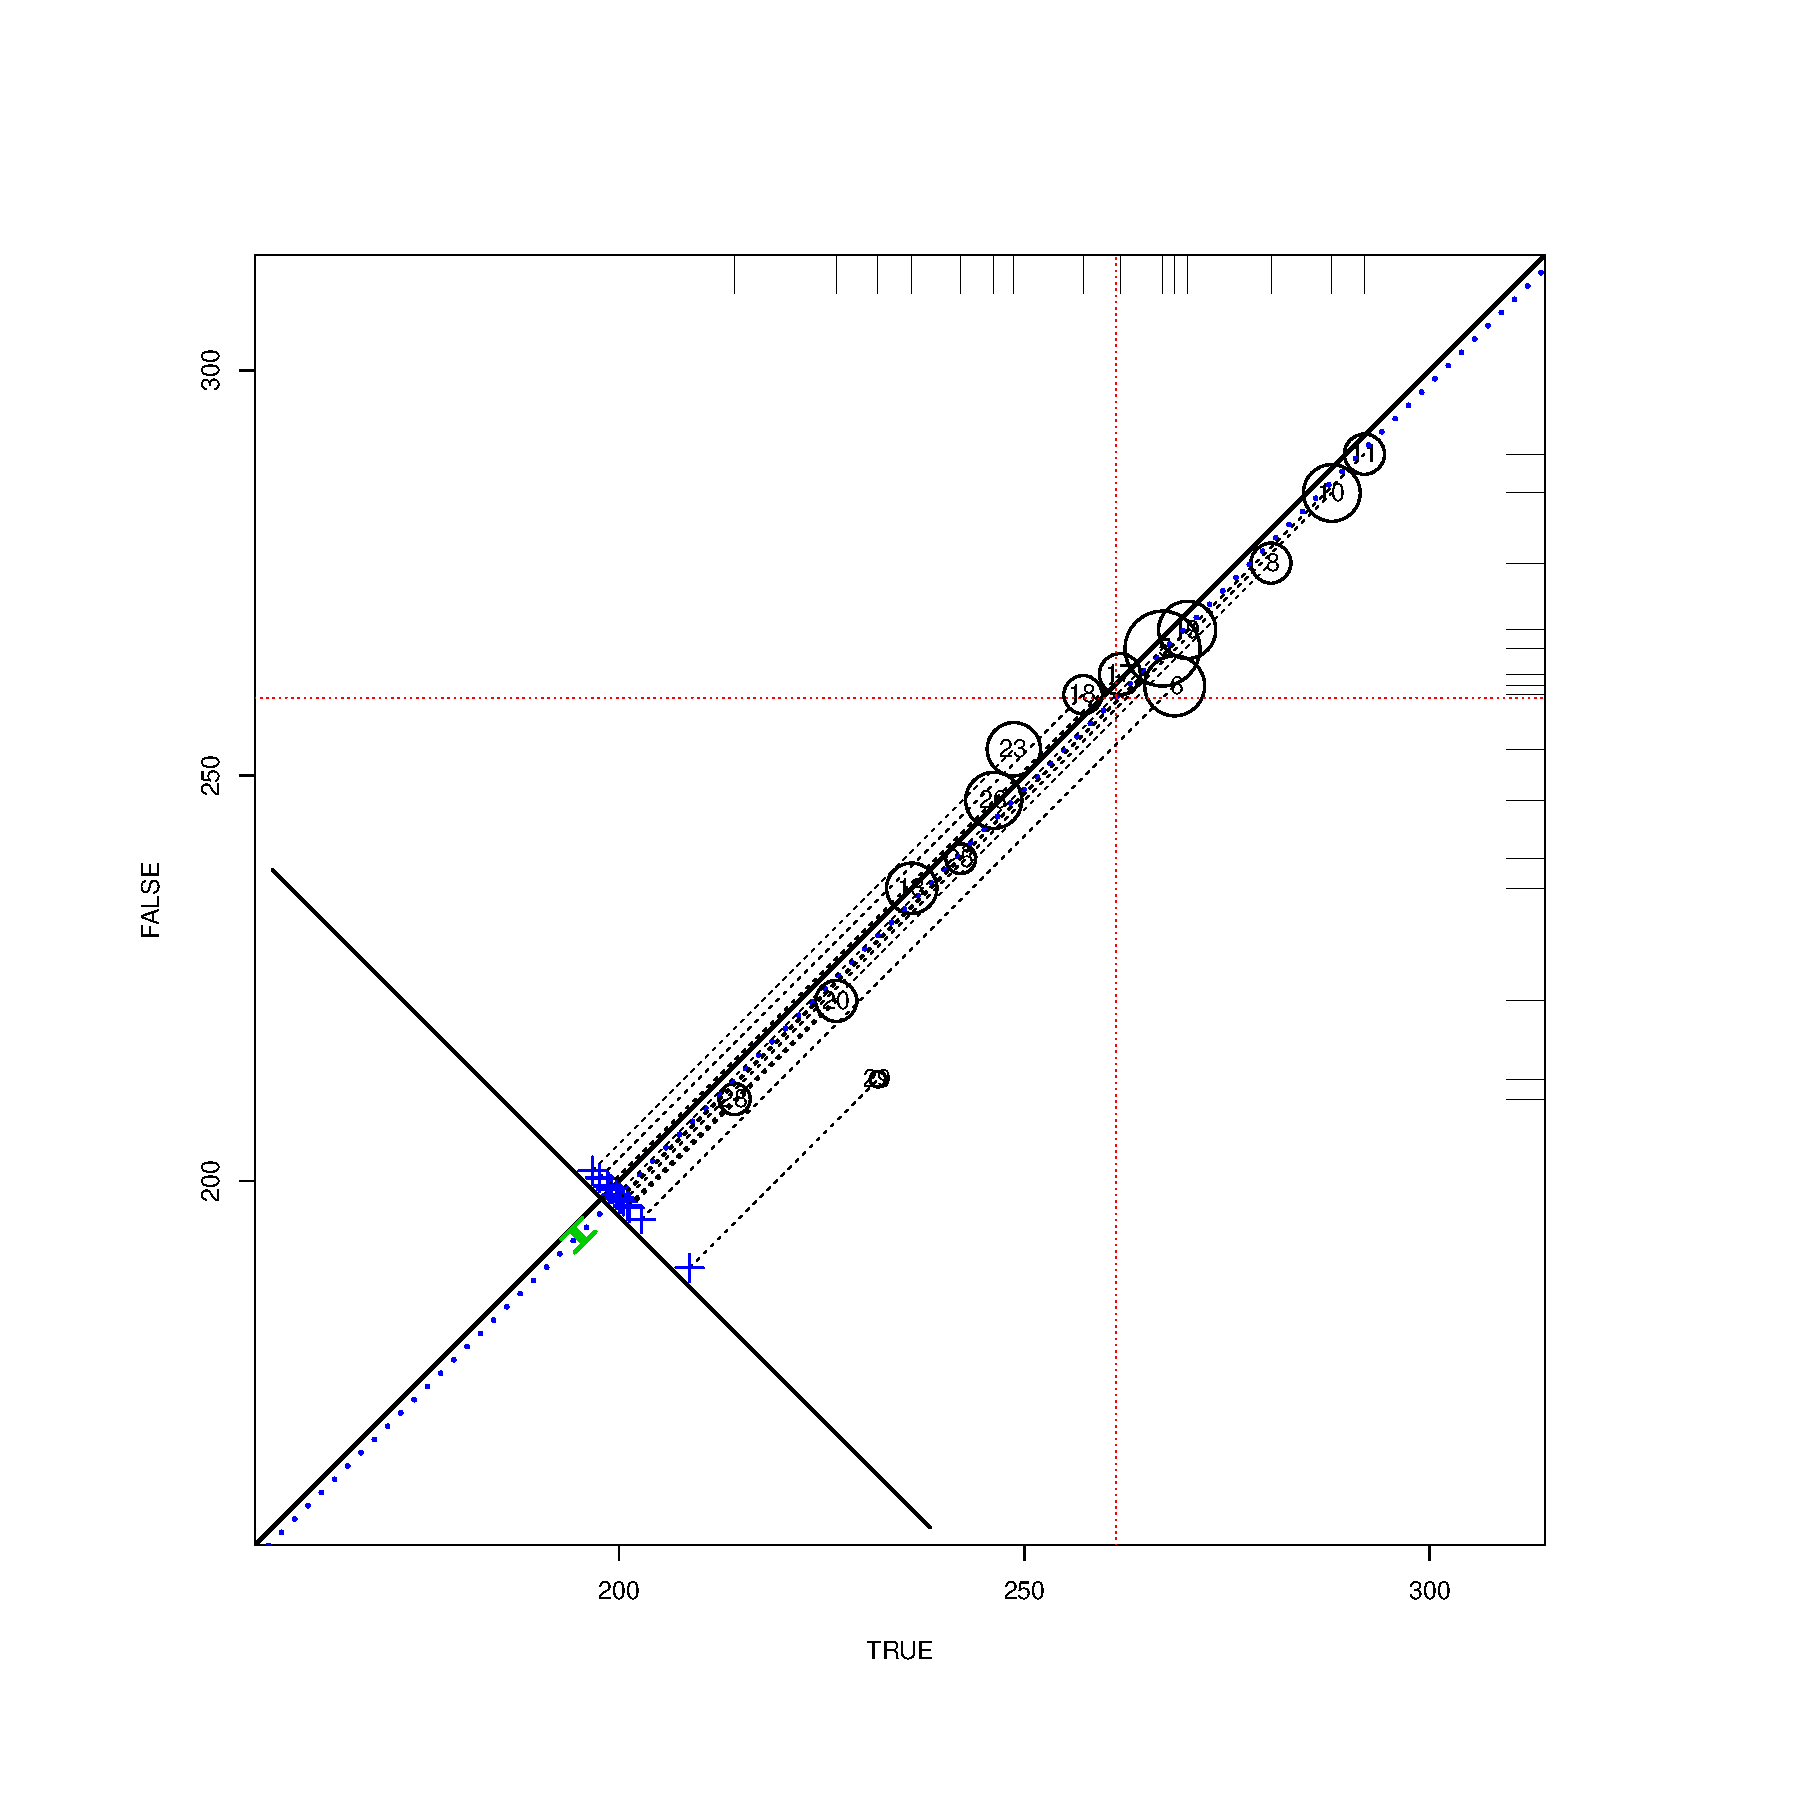
\includegraphics[height=.4\textheight,width=.4\textheight]{../Figures2009/g8read-circpsa-tree.pdf}
\caption{Propensity score assessment plot for classification tree stratification: Grade 8 reading}
\end{center}
\end{figure}

% latex table generated in R 3.0.2 by xtable 1.7-1 package
% Sun Feb 23 12:20:17 2014
\begin{table}[h!]
\centering
\caption{Classification trees stratification results for grade 8 reading} 
\label{g8read-circpsa-tree}
\begin{tabular}{lrr@{\extracolsep{.2cm}}rr}
  \hline
   & \multicolumn{2}{c}{Public} & \multicolumn{2}{c}{Charter} \\ \cline{2-3} \cline{4-5} Strata & Mean & n & Mean & n \\ \hline
5 & 265.67 & 14613 & 267.03 & 381 \\ 
  6 & 261.08 & 8482 & 268.53 & 163 \\ 
  8 & 276.22 & 3089 & 280.42 &  79 \\ 
  10 & 284.87 & 7238 & 287.92 & 265 \\ 
  11 & 289.66 & 3063 & 291.96 & 157 \\ 
  13 & 236.11 & 5341 & 236.11 & 233 \\ 
  17 & 262.51 & 3239 & 261.80 & 188 \\ 
  18 & 259.98 & 2725 & 257.24 & 112 \\ 
  19 & 267.97 & 7196 & 270.08 & 453 \\ 
  20 & 222.21 & 3127 & 226.81 & 250 \\ 
  23 & 253.26 & 5887 & 248.70 & 529 \\ 
  25 & 239.75 & 1400 & 242.16 & 119 \\ 
  26 & 246.96 & 6535 & 246.22 & 766 \\ 
  28 & 210.10 & 1606 & 214.26 &  84 \\ 
  29 & 212.56 & 269 & 231.94 &  33 \\ 
   \hline
\end{tabular}
\end{table}




%==================== Appendix G ====================================================================
\clearpage
\addcontentsline{toc}{subsection}{Appendix G: Multilevel PSA Covariate Balance Plots}
\section*{Appendix G\\Multilevel PSA Covariate Balance Plots}
\label{appendixG}

% Grade 4 math
\begin{figure}[h!]
\begin{center}
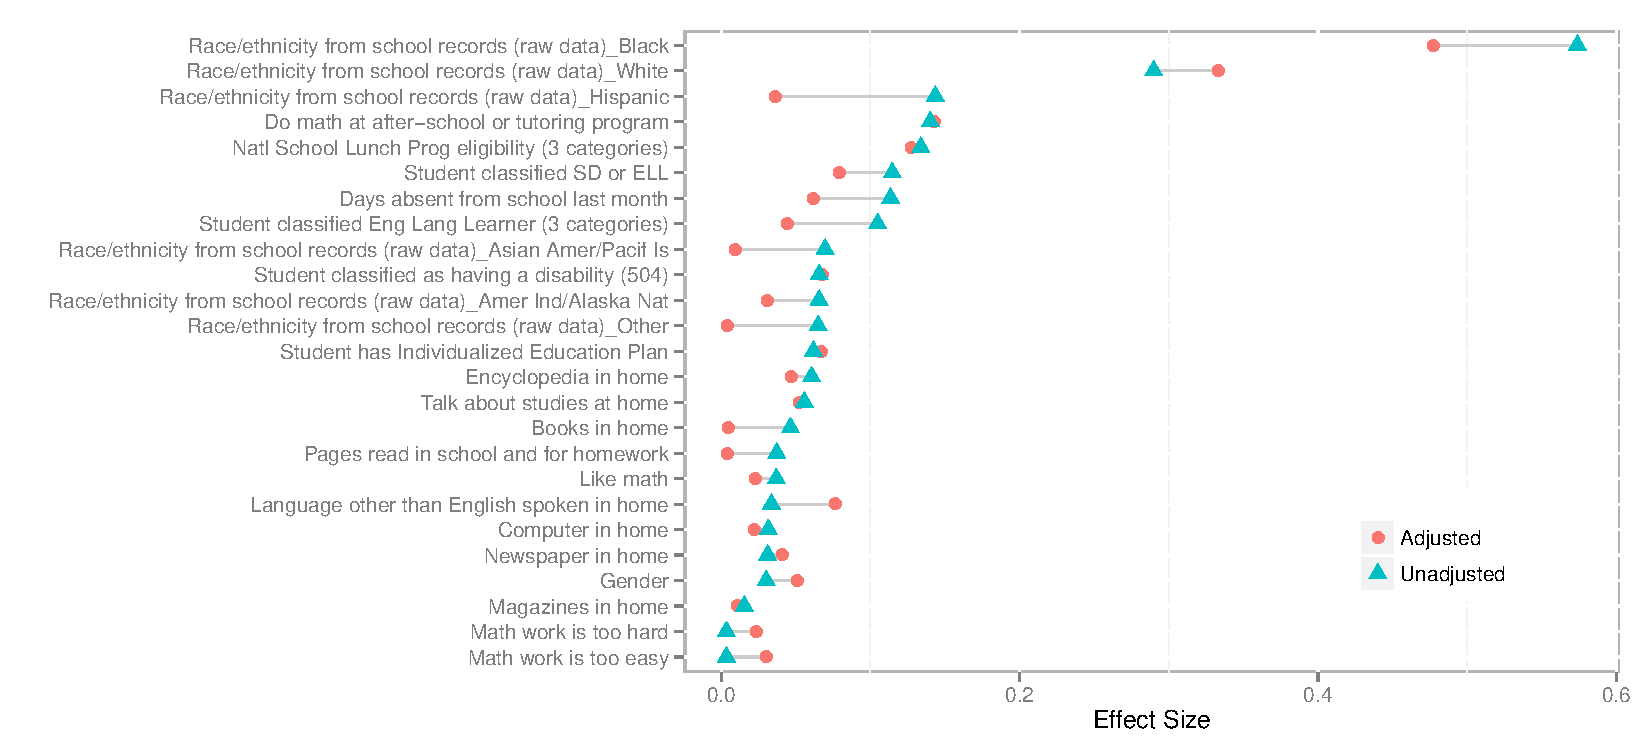
\includegraphics[width=\textwidth]{../Figures2009/g4math-mlpsa-lr-balance.pdf}
\caption{Multilevel PSA covariate balance plot logistic regression: Grade 4 math}
\end{center}
\end{figure}

\begin{figure}[h!]
\begin{center}
\includegraphics[width=\textwidth]{../Figures2009/g4math-mlpsa-lrAIC-balance.pdf}
\caption{Multilevel PSA covariate balance plot logistic regression AIC: Grade 4 math}
\end{center}
\end{figure}

\begin{figure}[h!]
\begin{center}
\includegraphics[width=\textwidth]{../Figures2009/g4math-mlpsa-ctree-balance.pdf}
\caption{Multilevel PSA covariate balance plot classification tree: Grade 4 math}
\end{center}
\end{figure}

% Grade 4 reading
\begin{figure}[h!]
\begin{center}
\includegraphics[width=\textwidth]{../Figures2009/g4read-mlpsa-lr-balance.pdf}
\caption{Multilevel PSA covariate balance plot logistic regression: Grade 4 reading}
\end{center}
\end{figure}

\begin{figure}[h!]
\begin{center}
\includegraphics[width=\textwidth]{../Figures2009/g4read-mlpsa-lrAIC-balance.pdf}
\caption{Multilevel PSA covariate balance plot logistic regression AIC: Grade 4 reading}
\end{center}
\end{figure}

\begin{figure}[h!]
\begin{center}
\includegraphics[width=\textwidth]{../Figures2009/g4read-mlpsa-ctree-balance.pdf}
\caption{Multilevel PSA covariate balance plot classification tree: Grade 4 reading}
\end{center}
\end{figure}

% Grade 8 math
\begin{figure}[h!]
\begin{center}
\includegraphics[width=\textwidth]{../Figures2009/g8math-mlpsa-lr-balance.pdf}
\caption{Multilevel PSA covariate balance plot logistic regression: Grade 8 math}
\end{center}
\end{figure}

\begin{figure}[h!]
\begin{center}
\includegraphics[width=\textwidth]{../Figures2009/g8math-mlpsa-lrAIC-balance.pdf}
\caption{Multilevel PSA covariate balance plot logistic regression AIC: Grade 8 math}
\end{center}
\end{figure}

\begin{figure}[h!]
\begin{center}
\includegraphics[width=\textwidth]{../Figures2009/g8math-mlpsa-ctree-balance.pdf}
\caption{Multilevel PSA covariate balance plot classification tree: Grade 8 math}
\end{center}
\end{figure}

% Grade 8 reading
\begin{figure}[h!]
\begin{center}
\includegraphics[width=\textwidth]{../Figures2009/g8read-mlpsa-lr-balance.pdf}
\caption{Multilevel PSA covariate balance plot logistic regression: Grade 8 reading}
\end{center}
\end{figure}

\begin{figure}[h!]
\begin{center}
\includegraphics[width=\textwidth]{../Figures2009/g8read-mlpsa-lrAIC-balance.pdf}
\caption{Multilevel PSA covariate balance plot logistic regression AIC: Grade 8 reading}
\end{center}
\end{figure}

\begin{figure}[h!]
\begin{center}
\includegraphics[width=\textwidth]{../Figures2009/g8read-mlpsa-ctree-balance.pdf}
\caption{Multilevel PSA covariate balance plot classification tree: Grade 8 reading}
\end{center}
\end{figure}


%==================== Appendix H ====================================================================
\clearpage
\addcontentsline{toc}{subsection}{Appendix H: Multilevel PSA Results}
\section*{Appendix H\\Multilevel PSA Results}
\label{appendixH}

% Grade 4 reading
\begin{figure}[h!]
\begin{center}
\includegraphics[width=\textwidth]{../Figures2009/g4read-mlpsa-lr-circ.pdf}
\caption{Multilevel PSA assessment plot logistic regression: Grade 4 reading}
\end{center}
\end{figure}

\begin{figure}[h!]
\begin{center}
\includegraphics[width=\textwidth]{../Figures2009/g4read-mlpsa-lr-diff.pdf}
\caption{Multilevel PSA difference plot logistic regression: Grade 4 reading}
\end{center}
\end{figure}

\begin{figure}[h!]
\begin{center}
\includegraphics[width=\textwidth]{../Figures2009/g4read-mlpsa-lrAIC-circ.pdf}
\caption{Multilevel PSA assessment plot logistic regression AIC: Grade 4 reading}
\end{center}
\end{figure}

\begin{figure}[h!]
\begin{center}
\includegraphics[width=\textwidth]{../Figures2009/g4read-mlpsa-lrAIC-diff.pdf}
\caption{Multilevel PSA difference plot logistic regression AIC: Grade 4 reading}
\end{center}
\end{figure}

\begin{figure}[h!]
\begin{center}
\includegraphics[width=\textwidth]{../Figures2009/g4read-mlpsa-ctree-circ.pdf}
\caption{Multilevel PSA assessment plot classification trees: Grade 4 reading}
\end{center}
\end{figure}

\begin{figure}[h!]
\begin{center}
\includegraphics[width=\textwidth]{../Figures2009/g4read-mlpsa-ctree-diff.pdf}
\caption{Multilevel PSA difference plot classification trees: Grade 4 reading}
\end{center}
\label{fig:g4read-mlpsa-ctree-diff}
\end{figure}

% Grade 8 math
\begin{figure}[h!]
\begin{center}
\includegraphics[width=\textwidth]{../Figures2009/g8math-mlpsa-lr-circ.pdf}
\caption{Multilevel PSA assessment plot logistic regression: Grade 8 math}
\end{center}
\end{figure}

\begin{figure}[h!]
\begin{center}
\includegraphics[width=\textwidth]{../Figures2009/g8math-mlpsa-lr-diff.pdf}
\caption{Multilevel PSA difference plot logistic regression: Grade 8 math}
\end{center}
\end{figure}

\begin{figure}[h!]
\begin{center}
\includegraphics[width=\textwidth]{../Figures2009/g8math-mlpsa-lrAIC-circ.pdf}
\caption{Multilevel PSA assessment plot logistic regression AIC: Grade 8 math}
\end{center}
\end{figure}

\begin{figure}[h!]
\begin{center}
\includegraphics[width=\textwidth]{../Figures2009/g8math-mlpsa-lrAIC-diff.pdf}
\caption{Multilevel PSA difference plot logistic regression AIC: Grade 8 math}
\end{center}
\end{figure}

\begin{figure}[h!]
\begin{center}
\includegraphics[width=\textwidth]{../Figures2009/g8math-mlpsa-ctree-circ.pdf}
\caption{Multilevel PSA assessment plot classification trees: Grade 8 math}
\end{center}
\end{figure}

\begin{figure}[h!]
\begin{center}
\includegraphics[width=\textwidth]{../Figures2009/g8math-mlpsa-ctree-diff.pdf}
\caption{Multilevel PSA difference plot classification trees: Grade 8 math}
\end{center}
\label{fig:g8math-mlpsa-ctree-diff}
\end{figure}

% Grade 8 reading
\begin{figure}[h!]
\begin{center}
\includegraphics[width=\textwidth]{../Figures2009/g8read-mlpsa-lr-circ.pdf}
\caption{Multilevel PSA assessment plot logistic regression: Grade 8 reading}
\end{center}
\end{figure}

\begin{figure}[h!]
\begin{center}
\includegraphics[width=\textwidth]{../Figures2009/g8read-mlpsa-lr-diff.pdf}
\caption{Multilevel PSA difference plot logistic regression: Grade 8 reading}
\end{center}
\end{figure}

\begin{figure}[h!]
\begin{center}
\includegraphics[width=\textwidth]{../Figures2009/g8read-mlpsa-lrAIC-circ.pdf}
\caption{Multilevel PSA assessment plot logistic regression AIC: Grade 8 reading}
\end{center}
\end{figure}

\begin{figure}[h!]
\begin{center}
\includegraphics[width=\textwidth]{../Figures2009/g8read-mlpsa-lrAIC-diff.pdf}
\caption{Multilevel PSA difference plot logistic regression AIC: Grade 8 reading}
\end{center}
\end{figure}

\begin{figure}[h!]
\begin{center}
\includegraphics[width=\textwidth]{../Figures2009/g8read-mlpsa-ctree-circ.pdf}
\caption{Multilevel PSA assessment plot classification trees: Grade 8 reading}
\end{center}
\end{figure}

\begin{figure}[h!]
\begin{center}
\includegraphics[width=\textwidth]{../Figures2009/g8read-mlpsa-ctree-diff.pdf}
\caption{Multilevel PSA difference plot classification trees: Grade 8 reading}
\end{center}
\label{fig:g8read-mlpsa-ctree-diff}
\end{figure}


%\begin{singlespace}
%% latex table generated in R 3.0.2 by xtable 1.7-1 package
% Sun Feb 23 12:16:13 2014
\begin{longtable}{lrrr@{\extracolsep{.25cm}}rrc}
\caption{Multilevel PSA Results using Conditional Inference Trees: Grade 4 math} \\ 
   \hline & & \multicolumn{2}{c}{FALSE} & \multicolumn{2}{c}{TRUE} & \\ \cline{3-4} \cline{5-6} Level & Strata & Mean & n & Mean & n & Confidence Interval \\ \hline\endfirsthead \multicolumn{7}{l}{{...continued from previous page}}\\ \hline  & & \multicolumn{2}{c}{FALSE} & \multicolumn{2}{c}{TRUE} & \\ \cline{3-4} \cline{5-6} Level & Strata & Mean & n & Mean & n & Confidence Interval \\ \hline \endhead \endfoot \endlastfoot  \hline
AZ & Overall & 229.05 & 2814 & 225.07 & 226 & ( -7.698, -0.25) \\ 
   & 1 & 220.30 & 1634 & 215.58 &  83 &  \\ 
   & 2 & 240.40 & 1180 & 237.40 & 143 &  \\ 
   \hline
CA & Overall & 227.08 & 7099 & 224.91 & 170 & ( -6.426,  2.09) \\ 
   & 1 & 215.33 & 574 & 224.84 &  36 &  \\ 
   & 2 & 233.93 & 3848 & 229.80 &  57 &  \\ 
   & 3 & 219.98 & 2677 & 218.00 &  77 &  \\ 
   \hline
CO & Overall & 242.63 & 2516 & 245.67 & 132 & ( -5.508, 11.59) \\ 
   & 1 & 252.17 & 1540 & 253.17 & 114 &  \\ 
   & 2 & 226.75 & 976 & 233.19 &  18 &  \\ 
   \hline
DC & Overall & 218.84 & 1282 & 219.35 & 512 & ( -3.388,  4.41) \\ 
   & 1 & 245.74 & 294 & 240.12 &  48 &  \\ 
   & 2 & 214.47 & 322 & 218.15 & 229 &  \\ 
   & 3 & 211.30 & 666 & 212.20 & 235 &  \\ 
   \hline
DE & Overall & 239.29 & 2499 & 241.24 & 195 & ( -3.280,  7.18) \\ 
   & 1 & 228.64 & 889 & 230.41 & 107 &  \\ 
   & 2 & 232.74 & 445 & 234.26 &   6 &  \\ 
   & 3 & 248.40 & 568 & 249.20 &  26 &  \\ 
   & 4 & 251.78 & 597 & 255.35 &  56 &  \\ 
   \hline
FL & Overall & 240.16 & 4273 & 238.74 & 166 & ( -5.046,  2.20) \\ 
   & 1 & 251.88 & 1294 & 247.59 &  58 &  \\ 
   & 2 & 247.21 & 390 & 245.49 &  39 &  \\ 
   & 3 & 233.06 & 2589 & 233.14 &  69 &  \\ 
   \hline
GA & Overall & 232.69 & 3811 & 239.31 & 164 & (  1.825, 11.43) \\ 
   & 1 & 253.95 & 147 & 261.10 &   5 &  \\ 
   & 2 & 233.67 & 350 & 236.84 &  20 &  \\ 
   & 3 & 255.04 & 968 & 255.75 &  60 &  \\ 
   & 4 & 221.72 & 2346 & 231.36 &  79 &  \\ 
   \hline
HI & Overall & 236.20 & 2642 & 230.95 &  57 & (-12.175,  1.67) \\ 
   & 1 & 236.20 & 2642 & 230.95 &  57 &  \\ 
   \hline
ID & Overall & 240.96 & 2807 & 252.03 &  60 & (  0.836, 21.31) \\ 
   & 1 & 227.12 & 773 & 240.20 &   5 &  \\ 
   & 2 & 246.11 & 2034 & 256.44 &  55 &  \\ 
   \hline
IL & Overall & 232.75 & 4047 & 239.45 &  78 & (  1.083, 12.32) \\ 
   & 1 & 213.59 & 1079 & 217.26 &  41 &  \\ 
   & 2 & 243.67 & 1772 & 252.94 &  10 &  \\ 
   & 3 & 234.38 & 1196 & 240.12 &  27 &  \\ 
   \hline
LA & Overall & 229.43 & 2789 & 230.80 &  65 & ( -2.790,  5.53) \\ 
   & 1 & 229.43 & 2789 & 230.80 &  65 &  \\ 
   \hline
MA & Overall & 238.41 & 1864 & 228.12 &  50 & (-16.052, -4.52) \\ 
   & 1 & 239.41 & 978 & 229.67 &  37 &  \\ 
   & 2 & 237.28 & 886 & 226.38 &  13 &  \\ 
   \hline
MD & Overall & 238.63 & 3195 & 237.80 & 141 & ( -5.527,  3.87) \\ 
   & 1 & 258.67 & 1181 & 270.72 &  10 &  \\ 
   & 2 & 234.72 & 528 & 229.66 &  18 &  \\ 
   & 3 & 222.11 & 790 & 210.48 &  85 &  \\ 
   & 4 & 233.49 & 379 & 227.17 &   7 &  \\ 
   & 5 & 222.97 & 317 & 217.82 &  21 &  \\ 
   \hline
MI & Overall & 225.51 & 2767 & 229.25 & 211 & ( -2.811, 10.28) \\ 
   & 1 & 230.22 & 633 & 235.66 &  18 &  \\ 
   & 2 & 215.93 & 175 & 229.48 &  26 &  \\ 
   & 3 & 204.06 & 981 & 210.80 & 144 &  \\ 
   & 4 & 248.95 & 969 & 246.30 &  18 &  \\ 
   & 5 & 216.47 &   9 & 207.70 &   5 &  \\ 
   \hline
MN & Overall & 248.30 & 2969 & 253.45 & 106 & (  0.237, 10.07) \\ 
   & 1 & 223.41 & 281 & 230.24 &  34 &  \\ 
   & 2 & 251.14 & 2688 & 256.10 &  72 &  \\ 
   \hline
NC & Overall & 243.63 & 4035 & 242.27 &  92 & ( -7.267,  4.55) \\ 
   & 1 & 254.56 & 1998 & 251.50 &  58 &  \\ 
   & 2 & 241.40 & 490 & 256.37 &  25 &  \\ 
   & 3 & 229.93 & 1547 & 225.42 &   9 &  \\ 
   \hline
NJ & Overall & 246.86 & 2747 & 235.10 &  74 & (-20.975, -2.55) \\ 
   & 1 & 250.18 & 2370 & 237.40 &  15 &  \\ 
   & 2 & 237.74 & 154 & 226.48 &   5 &  \\ 
   & 3 & 223.53 & 223 & 220.26 &  54 &  \\ 
   \hline
NV & Overall & 234.83 & 2784 & 231.01 &  72 & (-11.091,  3.46) \\ 
   & 1 & 234.83 & 2784 & 231.01 &  72 &  \\ 
   \hline
NY & Overall & 225.58 & 849 & 230.20 &  57 & ( -1.313, 10.54) \\ 
   & 1 & 225.58 & 849 & 230.20 &  57 &  \\ 
   \hline
OH & Overall & 215.58 & 1105 & 214.62 & 118 & (-11.058,  9.13) \\ 
   & 1 & 214.25 & 885 & 218.18 & 112 &  \\ 
   & 2 & 221.47 & 220 & 198.93 &   6 &  \\ 
   \hline
PA & Overall & 237.81 & 3460 & 237.31 &  50 & ( -7.521,  6.53) \\ 
   & 1 & 248.64 & 2165 & 239.34 &  15 &  \\ 
   & 2 & 223.28 & 329 & 235.48 &   8 &  \\ 
   & 3 & 218.70 & 751 & 231.20 &  13 &  \\ 
   & 4 & 219.85 & 215 & 241.04 &  14 &  \\ 
   \hline
RI & Overall & 238.67 & 2404 & 241.31 &  79 & ( -3.149,  8.43) \\ 
   & 1 & 246.32 & 1771 & 247.64 &  21 &  \\ 
   & 2 & 218.83 & 633 & 224.90 &  58 &  \\ 
   \hline
TX & Overall & 238.98 & 6162 & 230.83 &  91 & (-15.817, -0.48) \\ 
   & 1 & 235.46 & 3664 & 231.55 &  75 &  \\ 
   & 2 & 244.22 & 2498 & 229.77 &  16 &  \\ 
   \hline
UT & Overall & 239.88 & 2921 & 244.66 & 197 & ( -1.178, 10.73) \\ 
   & 1 & 219.92 & 673 & 228.28 &  20 &  \\ 
   & 2 & 245.59 & 2248 & 249.34 & 177 &  \\ 
   \hline
WI & Overall & 237.59 & 3637 & 242.59 & 136 & (  0.041,  9.96) \\ 
   & 1 & 248.66 & 2255 & 257.62 &  31 &  \\ 
   & 2 & 219.72 & 1119 & 217.56 &  67 &  \\ 
   & 3 & 226.36 &  46 & 228.04 &  17 &  \\ 
   & 4 & 223.30 & 217 & 226.81 &  21 &  \\ 
   \hline \multicolumn{7}{l}{\textit{Note:} Removed 7816 (10\%) rows due to insufficent data within a given strata.} \\\hline
\label{g4math-mlpsa-ctree}
\end{longtable}

%\clearpage
%% latex table generated in R 3.0.0 by xtable 1.7-1 package
% Thu May 30 09:15:19 2013
\begin{longtable}{lrrr@{\extracolsep{.25cm}}rrc}
\caption{Multilevel PSA Results using Conditional Inference Trees: Grade 4 read} \\ 
   \hline & & \multicolumn{2}{c}{TRUE} & \multicolumn{2}{c}{FALSE} & \\ \cline{3-4} \cline{5-6} Level & Strata & Mean & n & Mean & n & Confidence Interval \\ \hline\endfirsthead \multicolumn{7}{l}{{...continued from previous page}}\\ \hline  & & \multicolumn{2}{c}{TRUE} & \multicolumn{2}{c}{FALSE} & \\ \cline{3-4} \cline{5-6} Level & Strata & Mean & n & Mean & n & Confidence Interval \\ \hline \endhead \endfoot \endlastfoot  \hline
AZ & Overall & 210.03 & 240 & 211.64 & 2640 & ( -5.42,  8.65) \\ 
   & 1 & 216.79 & 208 & 219.13 & 2007 &  \\ 
   & 2 & 187.50 &  32 & 186.70 & 633 &  \\ 
   \hline
CA & Overall & 199.96 & 183 & 204.44 & 7659 & ( -2.63, 11.59) \\ 
   & 1 & 216.07 &  26 & 225.03 & 2463 &  \\ 
   & 2 & 190.72 & 123 & 194.38 & 4570 &  \\ 
   & 3 & 204.92 &  34 & 198.37 & 626 &  \\ 
   \hline
CO & Overall & 220.93 & 143 & 225.84 & 2742 & ( -3.75, 13.57) \\ 
   & 1 & 236.36 & 120 & 237.69 & 1692 &  \\ 
   & 2 & 194.89 &  23 & 205.83 & 1050 &  \\ 
   \hline
DC & Overall & 201.20 & 541 & 202.62 & 1307 & ( -2.72,  5.56) \\ 
   & 1 & 220.08 &  48 & 228.91 & 336 &  \\ 
   & 2 & 193.93 & 296 & 194.00 & 674 &  \\ 
   & 3 & 200.79 & 197 & 199.12 & 297 &  \\ 
   \hline
DE & Overall & 225.22 & 216 & 225.78 & 2557 & ( -5.15,  6.28) \\ 
   & 1 & 235.52 &  92 & 237.00 & 1106 &  \\ 
   & 2 & 221.95 &  11 & 219.88 & 594 &  \\ 
   & 3 & 209.15 &  80 & 213.35 & 459 &  \\ 
   & 4 & 221.27 &  33 & 218.46 & 398 &  \\ 
   \hline
FL & Overall & 224.61 & 183 & 222.87 & 4168 & ( -5.60,  2.10) \\ 
   & 1 & 217.18 &  21 & 213.55 & 1290 &  \\ 
   & 2 & 224.15 &  48 & 218.04 & 1356 &  \\ 
   & 3 & 226.57 &  33 & 227.79 & 377 &  \\ 
   & 4 & 234.03 &  19 & 237.33 & 461 &  \\ 
   & 5 & 231.42 &  62 & 236.31 & 684 &  \\ 
   \hline
GA & Overall & 217.76 & 173 & 214.89 & 3606 & ( -7.39,  1.64) \\ 
   & 1 & 237.09 &  48 & 231.69 & 974 &  \\ 
   & 2 & 201.14 &  30 & 198.20 & 1074 &  \\ 
   & 3 & 216.90 &  95 & 215.65 & 1558 &  \\ 
   \hline
HI & Overall & 210.69 &  78 & 210.96 & 2855 & ( -8.11,  8.64) \\ 
   & 1 & 237.23 &  22 & 225.88 & 382 &  \\ 
   & 2 & 206.46 &  56 & 208.57 & 2473 &  \\ 
   \hline
ID & Overall & 234.12 &  72 & 220.45 & 2931 & (-20.11, -7.23) \\ 
   & 1 & 239.78 &  25 & 223.67 & 984 &  \\ 
   & 2 & 248.74 &  38 & 234.36 & 650 &  \\ 
   & 3 & 222.06 &   9 & 210.64 & 1297 &  \\ 
   \hline
IL & Overall & 211.68 &  81 & 212.89 & 4301 & ( -6.19,  8.60) \\ 
   & 1 & 195.88 &  42 & 193.39 & 751 &  \\ 
   & 2 & 180.14 &   6 & 199.66 & 433 &  \\ 
   & 3 & 220.06 &  33 & 219.64 & 3117 &  \\ 
   \hline
LA & Overall & 200.08 &  73 & 208.21 & 3039 & (  2.30, 13.98) \\ 
   & 1 & 200.08 &  73 & 208.21 & 3039 &  \\ 
   \hline
MA & Overall & 235.30 &  54 & 229.11 & 3883 & (-13.01,  0.62) \\ 
   & 1 & 247.44 &   5 & 239.91 & 2154 &  \\ 
   & 2 & 208.52 &   9 & 213.34 & 607 &  \\ 
   & 3 & 226.94 &  40 & 217.39 & 1122 &  \\ 
   \hline
MD & Overall & 216.30 & 152 & 220.08 & 3246 & ( -0.84,  8.40) \\ 
   & 1 & 227.01 &  31 & 234.09 & 1692 &  \\ 
   & 2 & 214.52 &  36 & 211.98 & 774 &  \\ 
   & 3 & 196.61 &  85 & 199.75 & 780 &  \\ 
   \hline
MI & Overall & 211.75 & 213 & 211.70 & 3462 & ( -5.47,  5.37) \\ 
   & 1 & 222.09 &  30 & 225.35 & 1998 &  \\ 
   & 2 & 207.26 &  33 & 209.37 & 434 &  \\ 
   & 3 & 195.76 & 150 & 189.16 & 1030 &  \\ 
   \hline
MN & Overall & 227.12 & 109 & 222.42 & 3427 & (-22.49, 13.09) \\ 
   & 1 & 220.53 &   6 & 220.86 & 206 &  \\ 
   & 2 & 201.32 &  33 & 193.41 & 295 &  \\ 
   & 3 & 230.41 &  70 & 225.71 & 2926 &  \\ 
   \hline
NC & Overall & 220.55 & 104 & 218.95 & 4559 & ( -6.57,  3.37) \\ 
   & 1 & 219.75 &  28 & 223.55 & 575 &  \\ 
   & 2 & 230.21 &  30 & 237.26 & 1642 &  \\ 
   & 3 & 204.01 &  16 & 200.93 & 1731 &  \\ 
   & 4 & 241.19 &  30 & 215.99 & 611 &  \\ 
   \hline
NJ & Overall & 211.54 &  80 & 229.61 & 2764 & ( 12.64, 23.49) \\ 
   & 1 & 218.87 &  15 & 219.13 & 190 &  \\ 
   & 2 & 215.48 &  24 & 203.54 & 145 &  \\ 
   & 3 & 210.99 &  26 & 209.67 &  53 &  \\ 
   & 4 & 210.65 &  15 & 233.01 & 2376 &  \\ 
   \hline
NV & Overall & 215.72 &  75 & 209.42 & 2947 & (-15.54,  2.93) \\ 
   & 1 & 218.29 &  11 & 207.81 & 892 &  \\ 
   & 2 & 214.63 &  64 & 210.11 & 2055 &  \\ 
   \hline
NY & Overall & 221.53 &  68 & 207.60 & 876 & (-21.36, -6.49) \\ 
   & 1 & 221.53 &  68 & 207.60 & 876 &  \\ 
   \hline
OH & Overall & 201.92 & 136 & 203.24 & 1888 & ( -4.80,  7.42) \\ 
   & 1 & 209.00 &  11 & 211.51 & 978 &  \\ 
   & 2 & 195.16 & 125 & 195.33 & 910 &  \\ 
   \hline
OR & Overall & 219.32 &  56 & 217.80 & 3001 & (-10.78,  7.73) \\ 
   & 1 & 232.36 &  42 & 229.50 & 1619 &  \\ 
   & 2 & 203.81 &  14 & 203.87 & 1382 &  \\ 
   \hline
PA & Overall & 218.66 &  59 & 216.20 & 3713 & (-11.03,  6.11) \\ 
   & 1 & 218.66 &  59 & 216.20 & 3713 &  \\ 
   \hline
RI & Overall & 228.21 &  85 & 222.44 & 2566 & (-13.73,  2.20) \\ 
   & 1 & 234.09 &  21 & 230.58 & 1886 &  \\ 
   & 2 & 213.83 &  14 & 197.33 & 373 &  \\ 
   & 3 & 212.39 &  50 & 206.22 & 307 &  \\ 
   \hline
TX & Overall & 219.19 & 100 & 216.71 & 5827 & ( -7.33,  2.37) \\ 
   & 1 & 214.70 &  66 & 209.22 & 2658 &  \\ 
   & 2 & 223.01 &  34 & 223.09 & 3169 &  \\ 
   \hline
UT & Overall & 228.05 & 203 & 219.29 & 3057 & (-15.45, -2.07) \\ 
   & 1 & 225.05 &  13 & 197.63 & 660 &  \\ 
   & 2 & 228.83 & 190 & 224.92 & 2397 &  \\ 
   \hline
WI & Overall & 212.03 & 153 & 214.51 & 3878 & ( -2.75,  7.71) \\ 
   & 1 & 225.61 &  43 & 225.79 & 2468 &  \\ 
   & 2 & 180.75 &  48 & 188.57 & 545 &  \\ 
   & 3 & 193.65 &  25 & 204.17 & 601 &  \\ 
   & 4 & 202.04 &  17 & 202.49 &  48 &  \\ 
   & 5 & 197.65 &  20 & 190.38 & 216 &  \\ 
   \hline \multicolumn{7}{l}{\textit{Note:} Removed 5874 (6\%) rows due to insufficent data within a given strata.} \\\hline
\label{g4read-mlpsa-ctree}
\end{longtable}

%\clearpage
%% latex table generated in R 3.0.1 by xtable 1.7-1 package
% Tue Jun 11 08:07:12 2013
\begin{longtable}{lrrr@{\extracolsep{.25cm}}rrc}
\caption{Multilevel PSA Results using Conditional Inference Trees: Grade 8 math} \\ 
   \hline & & \multicolumn{2}{c}{FALSE} & \multicolumn{2}{c}{TRUE} & \\ \cline{3-4} \cline{5-6} Level & Strata & Mean & n & Mean & n & Confidence Interval \\ \hline\endfirsthead \multicolumn{7}{l}{{...continued from previous page}}\\ \hline  & & \multicolumn{2}{c}{FALSE} & \multicolumn{2}{c}{TRUE} & \\ \cline{3-4} \cline{5-6} Level & Strata & Mean & n & Mean & n & Confidence Interval \\ \hline \endhead \endfoot \endlastfoot  \hline
AZ & Overall & 276.44 & 2788 & 268.79 & 105 & (-17.602,   2.3) \\ 
   & 1 & 291.73 & 1394 & 272.25 &  19 &  \\ 
   & 2 & 260.02 & 1256 & 262.21 &  61 &  \\ 
   & 3 & 272.99 & 112 & 285.37 &   9 &  \\ 
   & 4 & 286.72 &  26 & 310.59 &  16 &  \\ 
   \hline
CA & Overall & 266.36 & 6459 & 271.98 & 525 & (  2.706,   8.5) \\ 
   & 1 & 271.35 & 2292 & 278.30 & 130 &  \\ 
   & 2 & 234.05 & 937 & 239.70 &  85 &  \\ 
   & 3 & 266.32 & 2409 & 271.25 & 250 &  \\ 
   & 4 & 290.26 & 821 & 294.29 &  60 &  \\ 
   \hline
CO & Overall & 287.36 & 2604 & 286.97 & 125 & ( -8.464,   7.7) \\ 
   & 1 & 267.84 & 851 & 252.01 &  22 &  \\ 
   & 2 & 296.54 & 1753 & 303.42 & 103 &  \\ 
   \hline
DC & Overall & 249.96 & 818 & 257.47 & 825 & (  2.577,  12.5) \\ 
   & 1 & 235.15 &  58 & 252.17 &  27 &  \\ 
   & 2 & 234.66 &  79 & 257.21 &  80 &  \\ 
   & 3 & 242.24 & 299 & 251.99 & 350 &  \\ 
   & 4 & 286.75 & 142 & 277.06 &  70 &  \\ 
   & 5 & 255.90 & 166 & 260.06 & 260 &  \\ 
   & 6 & 232.20 &  38 & 241.79 &  30 &  \\ 
   & 7 & 240.26 &  36 & 254.41 &   8 &  \\ 
   \hline
DE & Overall & 283.99 & 2275 & 290.37 & 201 & (  1.611,  11.1) \\ 
   & 1 & 279.59 & 1475 & 282.79 &  91 &  \\ 
   & 2 & 291.56 & 800 & 303.40 & 110 &  \\ 
   \hline
FL & Overall & 275.86 & 4012 & 280.59 & 272 & ( -0.078,   9.5) \\ 
   & 1 & 274.38 & 393 & 272.11 &  13 &  \\ 
   & 2 & 296.24 & 860 & 292.32 &  82 &  \\ 
   & 3 & 281.43 & 486 & 286.07 &  74 &  \\ 
   & 4 & 265.25 & 841 & 281.50 &  25 &  \\ 
   & 5 & 267.57 & 1432 & 273.00 &  78 &  \\ 
   \hline
GA & Overall & 263.18 & 2110 & 260.09 &  88 & (-10.868,   4.7) \\ 
   & 1 & 260.45 & 309 & 269.04 &  24 &  \\ 
   & 2 & 263.67 & 1801 & 258.49 &  64 &  \\ 
   \hline
HI & Overall & 273.61 & 2652 & 274.30 & 167 & ( -7.142,   8.5) \\ 
   & 1 & 267.90 & 105 & 256.78 &   5 &  \\ 
   & 2 & 285.84 & 273 & 292.77 &  50 &  \\ 
   & 3 & 266.45 & 1114 & 271.12 &  38 &  \\ 
   & 4 & 277.60 & 1160 & 273.99 &  74 &  \\ 
   \hline
ID & Overall & 293.06 & 1963 & 301.86 &  90 & (  1.983,  15.6) \\ 
   & 1 & 284.39 & 923 & 295.55 &  34 &  \\ 
   & 2 & 302.38 & 938 & 307.40 &  43 &  \\ 
   & 3 & 285.64 & 102 & 307.11 &  13 &  \\ 
   \hline
IL & Overall & 275.66 & 3897 & 269.00 & 110 & (-24.036,  10.7) \\ 
   & 1 & 260.89 & 2105 & 261.65 & 104 &  \\ 
   & 2 & 293.80 & 1792 & 278.03 &   6 &  \\ 
   \hline
IN & Overall & 286.56 & 2546 & 302.77 &  77 & (  8.810,  23.6) \\ 
   & 1 & 278.54 &  67 & 279.22 &  18 &  \\ 
   & 2 & 256.38 &  10 & 285.35 &  10 &  \\ 
   & 3 & 260.33 & 183 & 259.80 &  23 &  \\ 
   & 4 & 275.56 & 169 & 303.71 &   7 &  \\ 
   & 5 & 290.60 & 2117 & 307.93 &  19 &  \\ 
   \hline
LA & Overall & 272.53 & 2359 & 266.23 &  90 & (-13.079,   0.5) \\ 
   & 1 & 272.53 & 2359 & 266.23 &  90 &  \\ 
   \hline
MA & Overall & 294.76 & 3476 & 293.08 &  61 & ( -9.212,   5.8) \\ 
   & 1 & 291.70 & 1284 & 291.86 &   7 &  \\ 
   & 2 & 303.25 & 1476 & 298.17 &  28 &  \\ 
   & 3 & 282.89 & 716 & 284.89 &  26 &  \\ 
   \hline
MD & Overall & 282.19 & 2881 & 264.30 &  72 & (-25.666, -10.1) \\ 
   & 1 & 295.51 & 1816 & 263.47 &   9 &  \\ 
   & 2 & 260.63 & 1065 & 265.65 &  63 &  \\ 
   \hline
MI & Overall & 268.17 & 3206 & 260.58 & 160 & (-13.917,  -1.3) \\ 
   & 1 & 286.30 & 1954 & 271.50 &  34 &  \\ 
   & 2 & 242.02 & 1252 & 244.84 & 126 &  \\ 
   \hline
MN & Overall & 294.58 & 2655 & 295.27 &  80 & ( -7.845,   9.2) \\ 
   & 1 & 287.93 & 1556 & 285.83 &  18 &  \\ 
   & 2 & 308.66 & 987 & 313.60 &  45 &  \\ 
   & 3 & 263.16 & 112 & 263.83 &  17 &  \\ 
   \hline
NC & Overall & 281.95 & 4235 & 287.15 &  93 & ( -1.789,  12.2) \\ 
   & 1 & 255.14 & 170 & 232.76 &  12 &  \\ 
   & 2 & 266.64 & 1576 & 277.75 &  15 &  \\ 
   & 3 & 293.39 & 2489 & 296.87 &  66 &  \\ 
   \hline
OH & Overall & 278.88 & 3389 & 267.60 &  94 & (-17.227,  -5.3) \\ 
   & 1 & 283.22 & 2639 & 271.14 &  55 &  \\ 
   & 2 & 264.08 & 750 & 255.49 &  39 &  \\ 
   \hline
PA & Overall & 285.47 & 3192 & 277.46 & 109 & (-14.452,  -1.6) \\ 
   & 1 & 267.28 & 218 & 249.42 &  23 &  \\ 
   & 2 & 241.63 &  38 & 251.54 &  15 &  \\ 
   & 3 & 289.52 & 2764 & 281.15 &  54 &  \\ 
   & 4 & 260.52 & 172 & 265.35 &  17 &  \\ 
   \hline
TX & Overall & 283.52 & 5562 & 288.70 & 134 & ( -6.564,  16.9) \\ 
   & 1 & 287.92 & 4756 & 292.02 & 129 &  \\ 
   & 2 & 257.02 & 806 & 268.72 &   5 &  \\ 
   \hline
UT & Overall & 282.76 & 2681 & 292.19 & 110 & (  1.275,  17.6) \\ 
   & 1 & 282.11 & 1254 & 288.18 &  44 &  \\ 
   & 2 & 296.83 & 932 & 299.94 &  55 &  \\ 
   & 3 & 256.99 & 495 & 287.35 &  11 &  \\ 
   \hline
WI & Overall & 281.76 & 3182 & 264.85 & 231 & (-22.636, -11.2) \\ 
   & 1 & 299.57 & 1404 & 277.44 &  18 &  \\ 
   & 2 & 278.65 & 323 & 274.25 &  13 &  \\ 
   & 3 & 272.08 &  79 & 250.45 &  13 &  \\ 
   & 4 & 266.40 & 178 & 249.34 &  76 &  \\ 
   & 5 & 256.63 & 783 & 244.80 &  92 &  \\ 
   & 6 & 287.48 & 415 & 268.85 &  19 &  \\ 
   \hline \multicolumn{7}{l}{\textit{Note:} Removed 2600 (4\%) rows due to insufficent data within a given strata.} \\\hline
\label{g8math-mlpsa-ctree}
\end{longtable}

%\clearpage
%% latex table generated in R 3.0.1 by xtable 1.7-1 package
% Tue Jun 11 08:07:49 2013
\begin{longtable}{lrrr@{\extracolsep{.25cm}}rrc}
\caption{Multilevel PSA Results using Conditional Inference Trees: Grade 8 read} \\ 
   \hline & & \multicolumn{2}{c}{FALSE} & \multicolumn{2}{c}{TRUE} & \\ \cline{3-4} \cline{5-6} Level & Strata & Mean & n & Mean & n & Confidence Interval \\ \hline\endfirsthead \multicolumn{7}{l}{{...continued from previous page}}\\ \hline  & & \multicolumn{2}{c}{FALSE} & \multicolumn{2}{c}{TRUE} & \\ \cline{3-4} \cline{5-6} Level & Strata & Mean & n & Mean & n & Confidence Interval \\ \hline \endhead \endfoot \endlastfoot  \hline
AZ & Overall & 257.47 & 2680 & 261.71 &  92 & ( -6.904, 15.37) \\ 
   & 1 & 258.74 & 2361 & 262.02 &  65 &  \\ 
   & 2 & 251.15 & 306 & 262.71 &  18 &  \\ 
   & 3 & 210.84 &  13 & 211.83 &   9 &  \\ 
   \hline
CA & Overall & 247.26 & 6536 & 254.93 & 500 & (  4.973, 10.38) \\ 
   & 1 & 206.68 & 947 & 212.97 & 102 &  \\ 
   & 2 & 219.00 & 361 & 226.51 &  63 &  \\ 
   & 3 & 260.14 & 1178 & 271.89 &  45 &  \\ 
   & 4 & 270.44 & 956 & 275.94 &  61 &  \\ 
   & 5 & 247.90 & 1554 & 257.79 &  83 &  \\ 
   & 6 & 255.65 & 1540 & 260.44 & 146 &  \\ 
   \hline
CO & Overall & 264.41 & 2607 & 273.13 & 148 & (  4.021, 13.41) \\ 
   & 1 & 273.27 & 995 & 286.26 &  51 &  \\ 
   & 2 & 271.98 & 631 & 275.01 &  72 &  \\ 
   & 3 & 249.91 & 981 & 258.15 &  25 &  \\ 
   \hline
DC & Overall & 240.03 & 780 & 245.92 & 792 & ( -0.046, 11.83) \\ 
   & 1 & 236.24 & 399 & 245.16 & 445 &  \\ 
   & 2 & 230.53 & 224 & 239.42 & 156 &  \\ 
   & 3 & 250.11 &  21 & 244.28 &  33 &  \\ 
   & 4 & 297.63 &  55 & 278.73 &  15 &  \\ 
   & 5 & 249.99 &  81 & 249.99 & 143 &  \\ 
   \hline
DE & Overall & 264.73 & 2301 & 273.72 & 195 & (  4.388, 13.59) \\ 
   & 1 & 264.10 & 795 & 263.32 &  65 &  \\ 
   & 2 & 271.95 & 437 & 278.61 &  71 &  \\ 
   & 3 & 257.43 & 562 & 282.47 &  17 &  \\ 
   & 4 & 266.74 & 507 & 276.25 &  42 &  \\ 
   \hline
FL & Overall & 262.04 & 3883 & 268.60 & 281 & (  2.895, 10.22) \\ 
   & 1 & 256.79 & 1184 & 265.62 &  54 &  \\ 
   & 2 & 267.59 & 992 & 271.57 &  57 &  \\ 
   & 3 & 262.41 & 1707 & 268.91 & 170 &  \\ 
   \hline
GA & Overall & 258.28 & 3314 & 254.85 &  86 & (-13.986,  7.13) \\ 
   & 1 & 272.06 & 1474 & 265.06 &  11 &  \\ 
   & 2 & 248.00 & 1805 & 247.78 &  69 &  \\ 
   & 3 & 228.87 &  35 & 208.28 &   6 &  \\ 
   \hline
HI & Overall & 254.50 & 2693 & 251.88 & 172 & ( -7.888,  2.65) \\ 
   & 1 & 247.01 & 1575 & 243.23 &  69 &  \\ 
   & 2 & 268.19 & 683 & 268.50 &  79 &  \\ 
   & 3 & 258.58 & 435 & 255.26 &  24 &  \\ 
   \hline
ID & Overall & 264.05 & 2721 & 280.43 &  86 & ( 10.231, 22.53) \\ 
   & 1 & 254.71 & 1463 & 275.68 &  16 &  \\ 
   & 2 & 260.54 & 265 & 266.56 &  13 &  \\ 
   & 3 & 278.13 & 993 & 290.79 &  57 &  \\ 
   \hline
IL & Overall & 248.65 & 2228 & 249.43 & 102 & ( -4.449,  6.02) \\ 
   & 1 & 243.48 & 1064 & 247.00 &  69 &  \\ 
   & 2 & 253.54 & 1164 & 251.74 &  33 &  \\ 
   \hline
IN & Overall & 266.29 & 2554 & 260.93 &  77 & (-10.384, -0.33) \\ 
   & 1 & 268.49 & 2285 & 262.73 &  24 &  \\ 
   & 2 & 260.56 &  69 & 252.88 &  28 &  \\ 
   & 3 & 246.14 & 200 & 245.90 &  25 &  \\ 
   \hline
LA & Overall & 253.37 & 2374 & 250.34 &  89 & ( -8.927,  2.86) \\ 
   & 1 & 253.37 & 2374 & 250.34 &  89 &  \\ 
   \hline
MA & Overall & 269.76 & 3493 & 282.53 &  53 & (  4.911, 20.63) \\ 
   & 1 & 261.54 & 804 & 260.39 &  27 &  \\ 
   & 2 & 268.46 & 1760 & 286.93 &   9 &  \\ 
   & 3 & 279.41 & 929 & 293.75 &  17 &  \\ 
   \hline
MD & Overall & 246.30 & 1435 & 250.32 &  76 & ( -1.022,  9.07) \\ 
   & 1 & 249.79 & 1064 & 253.72 &  37 &  \\ 
   & 2 & 236.90 & 371 & 241.19 &  39 &  \\ 
   \hline
MI & Overall & 255.03 & 3155 & 256.46 & 162 & ( -4.285,  7.13) \\ 
   & 1 & 236.39 & 1224 & 237.56 & 125 &  \\ 
   & 2 & 267.81 & 1931 & 269.40 &  37 &  \\ 
   \hline
MN & Overall & 269.37 & 2710 & 274.13 &  78 & ( -2.784, 12.31) \\ 
   & 1 & 249.83 & 286 & 232.18 &  18 &  \\ 
   & 2 & 268.76 & 2040 & 276.67 &  31 &  \\ 
   & 3 & 286.81 & 384 & 292.31 &  29 &  \\ 
   \hline
NC & Overall & 258.13 & 4269 & 259.41 &  90 & ( -6.023,  8.59) \\ 
   & 1 & 252.16 & 2445 & 244.24 &  33 &  \\ 
   & 2 & 266.00 & 1824 & 279.39 &  57 &  \\ 
   \hline
OH & Overall & 262.97 & 3260 & 253.77 &  87 & (-15.357, -3.03) \\ 
   & 1 & 266.02 & 2544 & 254.84 &  55 &  \\ 
   & 2 & 252.37 & 716 & 250.06 &  32 &  \\ 
   \hline
PA & Overall & 263.48 & 3220 & 269.89 & 117 & (  1.242, 11.57) \\ 
   & 1 & 275.14 & 2254 & 281.11 &  33 &  \\ 
   & 2 & 241.16 & 247 & 244.00 &  18 &  \\ 
   & 3 & 232.88 & 443 & 246.19 &  25 &  \\ 
   & 4 & 243.24 & 276 & 245.54 &  41 &  \\ 
   \hline
RI & Overall & 257.86 & 2444 & 268.04 &  46 & (  0.850, 19.50) \\ 
   & 1 & 237.30 & 494 & 250.48 &  19 &  \\ 
   & 2 & 244.48 & 159 & 262.18 &  22 &  \\ 
   & 3 & 265.08 & 1791 & 273.64 &   5 &  \\ 
   \hline
TX & Overall & 257.71 & 5521 & 260.45 & 131 & ( -3.093,  8.58) \\ 
   & 1 & 254.33 & 3926 & 254.10 &  59 &  \\ 
   & 2 & 265.79 & 1595 & 275.65 &  72 &  \\ 
   \hline
UT & Overall & 263.69 & 2712 & 272.35 & 118 & (  3.596, 13.71) \\ 
   & 1 & 255.00 & 1538 & 264.44 &  43 &  \\ 
   & 2 & 274.69 & 1174 & 282.36 &  75 &  \\ 
   \hline
WI & Overall & 262.00 & 3131 & 255.63 & 216 & (-11.049, -1.68) \\ 
   & 1 & 244.61 & 965 & 238.63 & 156 &  \\ 
   & 2 & 270.75 & 2166 & 264.19 &  60 &  \\ 
   \hline \multicolumn{7}{l}{\textit{Note:} Removed 3807 (5\%) rows due to insufficent data within a given strata.} \\\hline
\label{g8read-mlpsa-ctree}
\end{longtable}

%\end{singlespace}



%==================== Appendix I ====================================================================
\clearpage
\addcontentsline{toc}{subsection}{Appendix I: Multilevel PSA Classification Tree Heat Maps}
\section*{Appendix I\\Multilevel PSA Classification Tree Heat Maps}
\label{appendixI}

\begin{figure}[h!]
\begin{center}
\includegraphics[height=.37\textheight]{../Figures2009/g4read-mlpsa-ctree-heat.pdf}
\caption{Heat map of relative importance of covariates from classification trees: Grade 4 reading}
\label{fig:g4read-mlpsa-ctree-heat}
\end{center}
\end{figure}

\begin{figure}[h!]
\begin{center}
\includegraphics[height=.37\textheight]{../Figures2009/g8math-mlpsa-ctree-heat.pdf}
\caption{Heat map of relative importance of covariates from classification trees: Grade 8 math}
\label{fig:g8math-mlpsa-ctree-heat}
\end{center}
\end{figure}

\begin{figure}[h!]
\begin{center}
\includegraphics[height=.37\textheight]{../Figures2009/g8read-mlpsa-ctree-heat.pdf}
\caption{Heat map of relative importance of covariates from classification trees: Grade 8 reading}
\label{fig:g8read-mlpsa-ctree-heat}
\end{center}
\end{figure}


%==================== Appendix J ====================================================================
\clearpage
\addcontentsline{toc}{subsection}{Appendix J: multilevelPSA R Package}
\section*{Appendix J\\multilevelPSA R Package}
\label{appendixJ}

The \texttt{multilevelPSA} R package was developed, in part, to conduct the analysis for this dissertation. It is available from the Comprehensive R Archive Network (CRAN) at \url{http://cran.r-project.org/web/packages/multilevelPSA}. The latest version can be installed using the \texttt{install.packages} function in R:

\begin{verbatim}
> install.packages('multilevelPSA', repos='http://cran.r-project.org')
\end{verbatim}

The following list provides brief descriptions of the key functions in the \texttt{multilevelPSA} package. More information is available vis-\`a-vis the R help system.

\renewcommand{\descriptionlabel}[1]{\hspace{\labelsep}\textbf{\texttt{#1}}}
\begin{description}
\item[getPropensityScores] Returns a data frame with two columns corresponding to the level 2 variable and the fitted value from the logistic regression.
\item[getStrata] Returns a data frame with two columns corresponding to the level 2 variable and the leaves from the conditional inference trees.
\item[loess.plot] Loess plot with density distributions for propensity scores and outcomes on top and right, respectively.
\item[missing.plot] Returns a heat map graphic representing missingness of variables grouped by the given grouping vector.
\item[mlpsa] This function will perform phase II of the multilevel propensity score analysis.
\item[plot.mlpsa] Creates the multilevel assessment plot.
\item[mlpsa.circ.plot] Plots the results of a multilevel propensity score model.
\item[mlpsa.ctree] Estimates propensity scores using the recursive partitioning in a conditional inference framework.
\item[mlpsa.difference.plot] Creates a graphic summarizing the differences between treatment and comparison groups within and across level two clusters.
\item[mlpsa.distribution.plot] Plots distribution for either the treatment or comparison group.
\item[mlpsa.logistic] Estimates propensity scores using logistic regression.
\item[psrange] Estimates models with increasing number of comparison subjects starting from 1:1 to using all available comparison group subjects.
\item[plot.psrange] Plots the results of \texttt{psrange}.
\item[tree.plot] Heat map representing variables used in a conditional inference tree across level 2 variables.
\end{description}

%==================== Appendix K ====================================================================
\clearpage
\addcontentsline{toc}{subsection}{Appendix K: Simulating Propensity Score Ranges}
\section*{Appendix K\\Simulating Propensity Score Ranges}
\label{appendixK}

\begin{singlespace}

\noindent The \texttt{getSimulatedData} function is what is used to simulate covariates with varying overlap.

\begin{verbatim}
getSimulatedData <- function(nvars = 3, 
    ntreat = 100, treat.mean = 0.6, treat.sd = 0.5, 
    ncontrol = 1000, control.mean = 0.4, control.sd = 0.5) {
    if (length(treat.mean) == 1) {
        treat.mean = rep(treat.mean, nvars)
    }
    if (length(treat.sd) == 1) {
        treat.sd = rep(treat.sd, nvars)
    }
    if (length(control.mean) == 1) {
        control.mean = rep(control.mean, nvars)
    }
    if (length(control.sd) == 1) {
        control.sd = rep(control.sd, nvars)
    }
    
    df <- c(rep(0, ncontrol), rep(1, ntreat))
    for (i in 1:nvars) {
        df <- cbind(df, c(
            rnorm(ncontrol, mean = control.mean[1], sd = control.sd[1]), 
            rnorm(ntreat, mean = treat.mean[1], sd = treat.sd[1])
        ) )
    }
    df <- as.data.frame(df)
    names(df) <- c("treat", letters[1:nvars])
    return(df)
}
\end{verbatim}

\noindent The following code was used to create Figure \ref{fig:psranges} in Chapter 5 which represents moderate overlap but some separation in covariates between treatment and control.


\begin{verbatim}
set.seed(2112)
df.psrange <- getSimulatedData(ncontrol = 1000, nvars=1,
                               treat.mean=0.6, treat.sd=0.4,
                               control.mean=0.4, control.sd=0.4)
psrange.test <- psrange(df.psrange, df.psrange$treat, treat ~ ., 
                        samples = seq(100, 1000, by = 100), nboot = 20)
plot(psrange.test)
\end{verbatim}

\noindent The following simulates covariates with perfect overlap (i.e. the differences between covariate values between treatment and control is random).

\begin{verbatim}
df.overlap <- getSimulatedData(ncontrol = 1000, nvars=1,
                               treat.mean=0.5, treat.sd=0.4,
                               control.mean=0.5, control.sd=0.4)
psrange.overlap <- psrange(df.overlap, df.overlap$treat, treat ~ ., 
                           samples = seq(100, 1000, by = 100), nboot = 20)
plot(psrange.overlap)
\end{verbatim}

\begin{figure}[h!]
\begin{center}
\includegraphics[width=\textwidth]{../Figures2009/PSRanges-Overlap.pdf}
\caption{Propensity score ranges for varying treatment-to-control ratios with perfect overlapping covariate}
\end{center}
\end{figure}

\noindent The following simulates covariates with almost no overlap (i.e. the covariate values can almost perfectly predict treatment placement).

\begin{verbatim}
df.nooverlap <- getSimulatedData(ncontrol = 1000, nvars=1,
                                 treat.mean=0.2, treat.sd=0.4,
                                 control.mean=0.8, control.sd=0.4)
psrange.nooverlap <- psrange(df.nooverlap, df.nooverlap$treat, treat ~ ., 
                             samples = seq(100, 1000, by = 100), nboot = 20)
plot(psrange.nooverlap)
\end{verbatim}

\begin{figure}[h!]
\begin{center}
\includegraphics[width=\textwidth]{../Figures2009/PSRanges-NoOverlap.pdf}
\caption{Propensity score ranges for varying treatment-to-control ratios with non-overlapping covariate}
\end{center}
\end{figure}

\end{singlespace}


%==================== Appendix L ====================================================================
\clearpage
\addcontentsline{toc}{subsection}{Appendix L: Rubric for Rating the Quality of Charter School Laws}
\section*{Appendix L\\Rubric for Rating the Quality of Charter School Laws}
\label{appendixL}

This appendix contains the rubric used by the \citeA{NAPCS2010a} to rate the quality of state charter laws. For each state law rated, the law is given a score between 0 to 4 for each of the 20 components. The score for each component is then multiplied by the weight (ranging from 1 to 4) and those 20 values are summed to provide a total score. The range of possible scores for each law therefore ranges between 0 and 208.

\begin{singlespace}
\begin{landscape}
% latex table generated in R 3.1.1 by xtable 1.7-3 package
% Sun Aug 31 21:12:47 2014
{\smaller
\begin{longtable}{rp{2.2in}p{0.9in}p{0.9in}p{0.9in}p{0.9in}p{0.9in}c}
\caption{NAPCS Rubric for Rating the Quality of State Charter Laws} \\ 
   \hline & & \multicolumn{5}{c}{Scoring} & \\ \cline{3-7}& Component & \multicolumn{1}{c}{0} & \multicolumn{1}{c}{1} & \multicolumn{1}{c}{2} & \multicolumn{1}{c}{3} & \multicolumn{1}{c}{4} & Weight \\ \hline\endfirsthead \multicolumn{8}{l}{{...continued from previous page}}\\ \hline & & \multicolumn{5}{c}{Scoring} & \\ \cline{3-7}& Component & \multicolumn{1}{c}{0} & \multicolumn{1}{c}{1} & \multicolumn{1}{c}{2} & \multicolumn{1}{c}{3} & \multicolumn{1}{c}{4} & Weight \\ \hline \endhead   1 & No Caps, whereby: 1A. No limits are placed on the number of public charter schools or students (and no geographic limits). 1B. If caps exist, adequate room for growth.  & The state has a cap with no room for growth.  & The state has a cap with room for limited growth.  & The state has a cap with room for some growth.  & The state has a cap with room for ample growth. OR The state does not have a cap, but allows districts to restrict growth.  & The state does not have a cap. &   3 \\ 
   \hline
  2 & A Variety of Public Charter Schools Allowed, including: 2A. New start-ups. 2B. Public school conversions. 2C. Virtual schools.  & The state allows only public school conversions.  & Not Applicable  & The state allows new start-ups and public school conversions, but not virtual schools. OR The state allows only new start-ups.  & The state allows new start-ups and virtual schools, but not public school conversions.  & The state allows new start-ups, public school conversions, and virtual schools.  &   1 \\ 
   \hline
  3 & Multiple Authorizers Available, including: 3A. Two or more viable authorizing options for each applicant with direct application allowed to each authorizing option.  & The state has only a single viable authorizer option available, and there is no or almost no authorizing activity.  & The state has only a single viable authorizer option available, and there is some authorizing activity.  & The state has only a single viable authorizer option available, and there is considerable authorizing activity. OR The state allows two or more viable authorizing options for applicants in some but not all situations.  & The state allows two or more viable authorizing options for each applicant, but requires applicants to get preliminary approval from a state charter school advisory committee.  & The state allows two or more viable authorizing options for each applicant.  &   3 \\ 
   \hline \pagebreak \hline
  4 & Authorizer and Overall Program Accountability System Required, including: 4A. At least a registration process for local school boards to affirm their interest in chartering to the state. 4B. Application process for other eligible authorizing entities. 4C. Authorizer submission of annual report, which summarizes the agency’s authorizing activities as well as the performance of its school portfolio. 4D. A regular review process by authorizer oversight body. 4E. Authorizer oversight body with authority to sanction authorizers, including removal of authorizer right to approve schools. 4F. Periodic formal evaluation of overall state charter school program and outcomes.  & The state law includes none of the elements of the model law’s authorizer and overall program accountability system.  & The state law includes a small number of the elements of the model law’s authorizer and overall program accountability system.  & The state law includes some of the elements of the model law’s authorizer and overall program accountability system.  & The state law includes many of the elements of the model law’s authorizer and overall program accountability system.  & The state law includes all of the elements of the model law’s authorizer and overall program accountability system.  &   3 \\ 
   \hline
  5 & Adequate Authorizer Funding, including: 5A. Adequate funding from authorizing fees (or other sources). 5B. Guaranteed funding from authorizing fees (or from sources not subject to annual legislative appropriations). 5E. Prohibition on authorizers requiring schools to purchase services from them.  & The state law includes none of the model law’s provisions for adequate authorizer funding.  & The state law includes a small number of the model law’s provisions for adequate authorizer funding.  & The state law includes some of the model law’s provisions for adequate authorizer funding.  & The state law includes many of the model law’s provisions for adequate authorizer funding.  & The state law includes all of the model law’s provisions for adequate authorizer funding.  &   2 \\ 
   \hline
  6 & Transparent Charter Application, Review, and Decision-making Processes, including: 6A. Application elements for all schools. 6B. Additional application elements specific to conversion schools. 6C. Additional application elements specific to virtual schools. 6D. Additional application elements specific when using educational service providers. 6E. Additional application elements specific to replications. 6F. Authorizer-issued request for proposals (including application requirements and approval criteria). 6G. Thorough evaluation of each application including an in-person interview and a public meeting. 6H. All charter approval or denial decisions made in a public meeting, with authorizers stating reasons for denials in writing.  & The state law includes none of the model law’s provisions for transparent charter application, review, and decision- making processes.  & The state law includes a small number of the model law’s provisions for transparent charter application, review, and decision-making processes.  & The state law includes some of the model law’s provisions for transparent charter application, review, and decision-making processes.  & The state law includes many of the model law’s provisions for transparent charter application, review, and decision-making processes.  & The state law includes all of the model law’s provisions for transparent charter application, review, and decision- making processes.  &   4 \\ 
   \hline
  7 & Performance-Based Charter Contracts Required, with such contracts: 7A. Being created as a separate document from the application and executed by the governing board of the charter school and the authorizer. 7B. Defining the roles, powers, and responsibilities for the school and its authorizer. 7C. Defining academic and operational performance expectations by which the school will be judged, based on a performance framework that includes measures and metrics for, at a minimum, student academic proficiency and growth, achievement gaps, attendance, recurrent enrollment, postsecondary readiness (high schools), financial performance, and board stewardship (including compliance). 7D. Providing an initial term of five operating years (or a longer term with periodic high-stakes reviews). 7E. Including requirements addressing the unique environments of virtual schools, if applicable.  & The state law includes none of the model law’s provisions for performance- based charter contracts.  & The state law includes a small number of the model law’s provisions for performance- based charter contracts.  & The state law includes some of the model law’s provisions for performance- based charter contracts.  & The state law includes many of the model law’s provisions for performance- based charter contracts.  & The state law includes all of the model law’s provisions for performance- based charter contracts.  &   4 \\ 
   \hline
  8 & Comprehensive Charter School Monitoring and Data Collection Processes, including: 8A. The collection and analysis of student outcome data at least annually by authorizers (consistent with performance framework outlined in the contract). 8B. Financial accountability for charter schools (e.g., Generally Accepted Accounting Principles, independent annual audit reported to authorizer). 8C. Authorizer authority to conduct or require oversight activities. 8D. Annual school performance reports produced and made public by each authorizer. 8E. Authorizer notification to their schools of perceived problems, with opportunities to remedy such problems. 8F. Authorizer authority to take appropriate corrective actions or exercise sanctions short of revocation. & The state law includes none of the model law’s provisions for comprehensive charter school monitoring and data collection processes.  & The state law includes a small number of the model law’s provisions for comprehensive charter school monitoring and data collection processes.  & The state law includes some of the model law’s provisions for comprehensive charter school monitoring and data collection processes.  & The state law includes many of the model law’s provisions for comprehensive charter school monitoring and data collection processes.  & The state law includes all of the model law’s provisions for comprehensive charter school monitoring and data collection processes.  &   4 \\ 
   \hline
  9 & Clear Processes for Renewal, Nonrenewal, and Revocation Decisions, including: 9A. Authorizer must issue school performance renewal reports to schools whose charter will expire the following year. 9B. Schools seeking renewal must apply for it. 9C. Authorizers must issue renewal application guidance that provides an opportunity for schools to augment their performance record and discuss improvements and future plans. 9D. Clear criteria for renewal and nonrenewal/revocation. 9E. Authorizers must ground renewal decisions based on evidence regarding the school’s performance over the term of the charter contract (in accordance with the performance framework set forth in the charter contract). 9F. Authorizer authority to vary length of charter renewal contract terms based on performance or other issues. 9G. Authorizers must provide charter schools with timely notification of potential revocation or non-renewal (including reasons) and reasonable time to respond. 9H. Authorizers must provide charter schools with due process for nonrenewal and revocation decisions (e.g., public hearing, submission of evidence). 9I. All charter renewal, non-renewal, and revocation decisions made in a public meeting, with authorizers stating reasons for non-renewals and revocations in writing. 9J. Authorizers must have school closure protocols to ensure timely parent notification, orderly student and record transitions, and property and asset disposition.  & The state law includes none of the model law’s clear processes for renewal, nonrenewal, and revocation decisions.  & The state law includes a small number of the model law’s clear processes for renewal, nonrenewal, and revocation decisions.  & The state law includes some of the model law’s clear processes for renewal, nonrenewal, and revocation decisions.  & The state law includes many of the model law’s clear processes for renewal, nonrenewal, and revocation decisions.  & The state law includes all of the model law’s clear processes for renewal, nonrenewal, and revocation decisions.  &   4 \\ 
   \hline
 10 & Educational Service Providers Allowed, including: 10A. All types of educational service providers allowed to operate all or parts of charter schools. 10A. All types of educational service providers allowed to operate all or parts of charter schools. 10B. A performance contract between the independent public charter school board and the service provider is required. 10C. Existing and potential conflicts of interest between the two entities are required to be disclosed and explained in application.  & The state law prohibits charter schools from contracting with all types of educational service providers.  & The state law is silent regarding these arrangements. OR The state law prohibits contracting with certain types of educational service providers.  & The state law explicitly allows contracting with all types of educational service providers but does not include provisions regarding performance contracts and conflicts of interest.  & The state law explicitly allows contracting with all types of educational service providers and requires performance contracts or conflicts of interest provisions, but not both.  & The state law explicitly allows contracting with all types of educational service providers and has provisions regarding performance contracts and conflicts of interest.  &   2 \\ 
   \hline
 11 & Fiscally and Legally Autonomous Schools with Independent Public Charter School Boards, including: 11A. Fiscally and legally autonomous schools (e.g., schools have authority to receive and disburse funds, enter into contracts, and sue and be sued in their own names). 11B. School governing boards independent of the authorizer and created specifically to govern their charter school(s).  & The state law includes none of the model law’s provisions for fiscally and legally autonomous schools with independent public charter school boards.  & The state law includes a small number of the model law’s provisions for fiscally and legally autonomous schools with independent public charter school boards.  & The state law includes some of the model law’s provisions for fiscally and legally autonomous schools with independent public charter school boards. OR
The state law includes all of these provisions for some schools, but not others. & The state law includes many of the model law’s provisions for fiscally and legally autonomous schools with independent public charter school boards.  & The state law includes all of the model law’s provisions for fiscally of the model law’s provisions for fiscally and legally autonomous schools with independent public charter school boards.  &   3 \\ 
   \hline
 12 & Clear Student Recruitment, Enrollment, and Lottery Procedures, including: 12A. Open enrollment to any student in the state. 12B. Lottery requirements. 12C. Required enrollment preferences for previously enrolled students within conversions, prior year students within chartered schools, and siblings of enrolled students enrolled at a charter school. 12D. Optional enrollment preference for children of a school’s founders, governing board members, and full-time employees, not exceeding 10\% of the school’s total student population. & The state law includes none (or nearly none) of the model law’s requirements for student recruitment, enrollment, and lottery procedures.  & The state law includes a small number of the model law’s requirements for student recruitment, enrollment, and lottery procedures.  & The state law includes some of the model law’s requirements for student recruitment, enrollment, and lottery procedures.  & The state law includes many of the model law’s requirements for student recruitment, enrollment, and lottery procedures.  & The state law includes all of the model law’s requirements for student recruitment, enrollment, and lottery procedures.  &   1 \\ 
   \hline
 13 & Automatic Exemptions from Many State and District Laws and Regulations, including: 13A. Exemptions from all laws, except those covering health, safety, civil rights, student accountability, employee criminal history checks, open meetings, freedom of information, and generally accepted accounting principles. 13B. Exemption from state teacher certification requirements.  & The state law does not provide automatic exemptions from state and district laws and regulations, does not allow schools to apply for exemptions, and requires all of a school’s teachers to be certified.  & The state law allows schools to apply for exemptions from state and district laws and requires all of a school’s teachers to be certified. OR The state law does not provide automatic exemptions from many state and district laws and regulations and does not require any of a school’s teachers to be certified. OR The state law allows schools to apply for exemptions from state and district laws and requires some of a school’s teachers to be certified. & There were six variations for how state laws handled 13A and 13B that were included in this cell.  & The state law provides automatic exemptions from many state and district laws and regulations and requires some of a school’s teachers to be certified.  & The state law provides automatic exemptions from many state and district laws and regulations and does not require any of a school’s teachers to be certified.  &   3 \\ 
   \hline
 14 & Automatic Collective Bargaining Exemption, whereby: 14A. Charter schools authorized by non-local board authorizers are exempt from participation in district collective bargaining agreements. 14B. Charter schools authorized by local boards are exempt from participation in district collective bargaining agreements.  & The state law requires all charter schools to be part of district collective bargaining agreements, with no opportunity for exemptions.  & The state law requires all charter schools to be part of district collective bargaining agreements, but schools can apply for exemptions.  & The state law exempts some schools from district collective bargaining agreements, but not others.  & The state law exempts some schools from district collective bargaining agreements, but not others (but allows those not exempted to apply for exemptions).  & The state law does not require any charter schools to be part of district collective bargaining agreements.  &   3 \\ 
   \hline
 15 & Multi-School Charter Contracts and/or Multi-Charter Contract Boards Allowed, whereby an independent public charter school board may: 15A. Oversee multiple schools linked under a single contract with independent fiscal and academic accountability for each school. 15B. Hold multiple charter contracts with independent fiscal and academic accountability for each school.  & The state law prohibits these arrangements.  & The state law is silent regarding these arrangements. OR
The state law explicitly allows either of these arrangements but does not require each school to be independently accountable for fiscal and academic performance. OR The state law explicitly allows these arrangements for some schools but not others.  & The state law allows either of these arrangements, but only requires schools authorized by some entities to be independently accountable for fiscal and academic performance.  & Not Applicable  & The state law explicitly allows either of these arrangements and requires each school to be independently accountable for fiscal and academic performance.  &   1 \\ 
   \hline
 16 & Extra-Curricular and Interscholastic Activities Eligibility and Access, whereby: 16A. Laws or regulations explicitly state that charter school students and employees are eligible to participate in all interscholastic leagues, competitions, awards, scholarships, and recognition programs available to non-charter public school students and employees. 16B. Laws or regulations explicitly allow charter school students in schools not providing extra-curricular and interscholastic activities to have access to those activities at non-charter public schools for a fee by a mutual agreement.  & The state law prohibits charter eligibility and access.  & The state law is silent about charter eligibility and access.  & The state law provides either charter eligibility or access, but not both.  & The state law provides both charter eligibility and access to students, but not employees.  & The state law provides both charter eligibility and access.  &   1 \\ 
   \hline
 17 & Clear Identification of Special Education Responsibilities, including: 17A. Clarity regarding which entity is the local education agency (LEA) responsible for providing special education services. 17B. Clarity regarding funding for low-incident, high-cost services for charter schools (in the same amount and/or in a manner similar to other LEAs).  & The state law is silent about special education responsibilities and funding for low-incident, high-cost services.  & The state law addresses special education, but is unclear about responsibility for providing services and funding for low-incident, high-cost services.  & The state law is clear on either responsibility for providing services OR funding for low-incident, high-cost services, but not both.  & Not Applicable  & The state law clearly addresses responsibility for providing services and ensures state funding for low-incident, high-cost services.  &   2 \\ 
   \hline
 18 & Equitable Operational Funding and Equal Access to All State and Federal Categorical Funding, including: 18A. Equitable operational funding statutorily driven.18B. Equal access to all applicable categorical federal and state funding, and clear guidance on the pass-through of such funds. 18C. Funding for transportation similar to school districts.  & The state law includes none of the model law’s provisions for equitable operational funding and equal access to all state and federal categorical funding.  & The state law includes a small number of the model law’s provisions for equitable operational funding and equal access to all state and federal categorical funding.  & The state law includes some of the model law’s provisions for equitable operational funding and equal access to all state and federal categorical funding.  & The state law includes many of the model law’s provisions for equitable operational funding and equal access to all state and federal categorical funding.  & The state law includes all of the model law’s provisions for equitable operational funding and equal access to all state and federal categorical funding.  &   3 \\ 
   \hline
 19 & Equitable Access to Capital Funding and Facilities, including: 19A. A per-pupil facilities allowance which annually reflects actual average district capital costs. 19B. A state grant program for charter school facilities. 19C. A state loan program for charter school facilities. 19D. Equal access to tax-exempt bonding authorities or allow charter schools to have their own bonding authority. 19E. A mechanism to provide credit enhancement for public charter school facilities. 19F. Equal access to existing state facilities programs available to non-charter public schools. 19G. Right of first refusal to purchase or lease at or below fair market value a closed, unused, or underused public school facility or property. 19H. Prohibition of facility-related requirements stricter than those applied to traditional public schools.  & The state law includes none of the model law’s provisions for equitable access to capital funding and facilities.  & The state law includes a small number of the model law’s provisions for equitable access to capital funding and facilities.  & The state law includes some of the model law’s provisions for equitable access to capital funding and facilities.  & The state law includes many of the model law’s provisions for equitable access to capital funding and facilities.  & The state law includes all of the model law’s provisions for equitable access to capital funding and facilities.  &   3 \\ 
   \hline
 20 & Automatic Collective Bargaining Exemption, whereby: 20A. Charter schools have access to relevant state retirement systems available to other public schools.  20B. Charter schools have the option to participate (i.e., not required).  & The state law does not provide access to the relevant employee retirement systems.  & The state law requires participation in the relevant employee retirement systems for some schools, but denies access to these systems for other schools.  & The state law requires participation in the relevant employee retirement systems.  & The state law provides that charter schools have access and an option by virtue of how they hire their employees. OR The state law requires participation in the relevant employee retirement systems, unless at the time of application, a school has a retirement program which covers the employees or the employee is currently enrolled in another retirement program. OR The state law provides some charter schools with the option to participate in the relevant state employee retirement systems, but not others. & The state law provides access to relevant employee retirement systems, but does not require participation.  &   3 \\ 
   \hline
\hline
\label{NAPCSrubric}
\end{longtable}
}

\end{landscape}
\end{singlespace}

%==================== Appendix M ====================================================================
%\clearpage
\addcontentsline{toc}{subsection}{Appendix M: Matrix Plot of NAPCS Charter Law Scores and NAEP Charter School Effect Sizes}
\section*{Appendix M\\Matrix Plot of NAPCS Charter Law Scores and NAEP Charter School Effect Sizes}
\label{appendixM}

\begin{figure}[h!]
\begin{center}
\includegraphics[width=\textwidth]{../Figures2009/NAEPLawScoresMatrixPlot.pdf}
\caption{Matrix plot of NAPCS charter law scores and NAEP charter school effect sizes}
\end{center}
\end{figure}



%%%%% Left Overs %%%%%%%%%%%%%%%%%%%%%%%%%%%%%%%%%%%%%%%%%%%%%%%%%%%%
%%%%% Themeatic Map

%\newpage
%\addcontentsline{toc}{subsection}{Appendix B: Thematic Map of Number of Charter Schools in the United States}
%\subsection*{Appendix B\\Thematic Map of Number of Charter Schools by State in 2008}
%\label{appendixMap}
%\begin{figure}[h]
%\includegraphics[width=\textwidth]{../Figures/CharterMap.pdf}
%\caption{Thematic map of number of charter schools by state in 2008}
%\label{fig:charterMap}
%\end{figure}



\end{document}
